% 서울대학교 학사/석사/박사 학위논문
% LaTeX 양식 샘플
\RequirePackage{fix-cm} % documentclass 이전에 넣는다.
% oneside : 단면 인쇄용
% twoside : 양면 인쇄용
% ko : 국문 논문 작성
% master : 석사
% phd : 박사
% openright : 챕터가 홀수쪽에서 시작
\documentclass[oneside,ko,phd]{snuthesis}
%%%%%%%%%%%%%%%%%%%%%%%%%%%%%%%%%%%%%%%%%%%%%%%%%%%%%%%%%%%%%%%%%%%%%%%%%%%%%%
%%
%% Author: zeta709 (zeta709@gmail.com)
%% Releasedate: 2017/07/20
%%
%% 목차 양식을 변경하는 코드
%% * subfigure (subfig) package 사용 여부에 따라
%%   tocloft의 옵션을 다르게 지정해야 한다.
%% * Chapter 번호가 두 자리 수를 넘어가는 경우 다음과 같이
%%   필요한 만큼 "9"를 추가하면 된다.
%%   \settowidth{\mytmplen}{\bfseries\cftchappresnum9\cftchapaftersnum}
%%   아니면 \cftchapnumwidth를 직접 적당히 고치면 된다.
%%%%%%%%%%%%%%%%%%%%%%%%%%%%%%%%%%%%%%%%%%%%%%%%%%%%%%%%%%%%%%%%%%%%%%%%%%%%%%
%\usepackage[titles,subfigure]{tocloft} % when you use subfigure package
\usepackage[titles]{tocloft} % when you don't use subfigure package
\makeatletter
\if@snu@ko
	\renewcommand\cftchappresnum{제~}
	\renewcommand\cftchapaftersnum{~장}
	\renewcommand\cftfigpresnum{그림~}
	\renewcommand\cfttabpresnum{표~}
\else
	\renewcommand\cftchappresnum{Chapter~}
	\renewcommand\cftfigpresnum{Figure~}
	\renewcommand\cfttabpresnum{Table~}
\fi
\makeatother
\newlength{\mytmplen}
\settowidth{\mytmplen}{\bfseries\cftchappresnum\cftchapaftersnum}
\addtolength{\cftchapnumwidth}{\mytmplen}
\settowidth{\mytmplen}{\bfseries\cftfigpresnum\cftfigaftersnum}
\addtolength{\cftfignumwidth}{\mytmplen}
\settowidth{\mytmplen}{\bfseries\cfttabpresnum\cfttabaftersnum}
\addtolength{\cfttabnumwidth}{\mytmplen}
\makeatletter
\g@addto@macro\appendix{%
	\addtocontents{toc}{%
		\settowidth{\mytmplen}{\bfseries\protect\cftchappresnum\protect\cftchapaftersnum}%
		\addtolength{\cftchapnumwidth}{-\mytmplen}%
		\protect\renewcommand{\protect\cftchappresnum}{\appendixname~}%
		\protect\renewcommand{\protect\cftchapaftersnum}{}%
		\settowidth{\mytmplen}{\bfseries\protect\cftchappresnum\protect\cftchapaftersnum}%
		\addtolength{\cftchapnumwidth}{\mytmplen}%
	}%
}
\makeatother
 % SNU toc style

%%%%%%%%%%%%%%%%%%%%%%%%%%%%%%%%%%%%%%%%
%% 다른 패키지 로드
%% http://faq.ktug.or.kr/faq/pdflatex%B0%FAlatex%B5%BF%BD%C3%BB%E7%BF%EB
%% 필요에 따라 직접 수정 필요
\ifpdf
	\input glyphtounicode\pdfgentounicode=1 %type 1 font사용시
	\usepackage[pdftex]{graphicx}
	%\usepackage[pdftex,svgnames]{xcolor}
\else
	\usepackage[dvipdfmx]{graphicx}
	%\usepackage[dvipdfmx,svgnames]{xcolor}
\fi
	\usepackage{subcaption}
    \usepackage{float,pstricks,listings,stackengine,calligra}
    \usepackage{amsmath,amssymb,latexsym}
    \usepackage{booktabs,longtable,multicol,multirow,lscape,rotating}
    \usepackage{lipsum} % lorem ipsum
    
%%%%%%%%%%%%%%%%%%%%%%%%%%%%%%%%%%%%%%%%
%% 유저 커맨드
\newcommand{\source}[1]{{\raggedright \footnotesize 자료: {#1} \\ } }
\newcommand{\confer}[1]{{\raggedright \footnotesize 참고: {#1} \\ } }

%%%%%%%%%%%%%%%%%%%%%%%%%%%%%%%%%%%%%%%%
%% Biblatex을 이용한 한글 참고문헌 
\usepackage[%
    backend=biber, 
    bibencoding=utf8, 
    style=apa, 
    natbib=true, 
    citestyle=authoryear-comp, 
    bibstyle=authoryear,  
    maxcitenames=2, 
    maxbibnames=9, 
    language=auto, 
    autolang=other, 
    uniquelist=false 
]{biblatex}
\addbibresource{Bibliography.bib}
\renewcommand\nameyeardelim{, }	%% natbib command. natbib should be true.
\newcommand*{\myownetal}{\emph{et~al.}}
\DefineBibliographyStrings{english}{%
    bibliography = {참고문헌},
    andothers={\myownetal}{}
}
\AtEveryCitekey{%
  \ifkeyword{kobib}{%
    \renewcommand{\multinamedelim}{·}%
    \renewcommand{\finalnamedelim}{·}%
    \renewcommand*{\myownetal}{외}%
  }{}%
}
\AtEveryBibitem{%
  \renewbibmacro{in:}{}
  \ifkeyword{kobib}{%
    \renewcommand{\multinamedelim}{·}%
    \renewcommand{\finalnamedelim}{·}%
    \DeclareFieldFormat{journaltitle}{『#1』}%
    \DeclareFieldFormat[book]{title}{『#1』}%
    \DeclareFieldFormat[series]{title}{『#1』}%
    \DeclareFieldFormat{booktitle}{『#1』}%
  }{}%
}

%%%%%%%%%%%%%%%%%%%%%%%%%%%%%%%%%%%%%%%%
%% \title : 22pt로 나오는 큰 제목
%% \title* : 16pt로 나오는 작은 제목
\title{한국의 경제 및 교육의 기회불평등 분석}
\title*{~}

\academicko{경제학}
\departmentko{경제학부}

%% 저자 이름 Author's(Your) name
\author{오성재}
\author*{오~성~재} % Insert space for Hangul name.
%\author{Gildong Hong}
%\author*{Gildong Hong} % Same as \author.

%% 학번 Student number
\studentnumber{2015-30953}

%% 지도교수님 성함 Advisor's name
%% (?) Use Korean name for Korean professor.
\advisor{주병기}
\advisor*{주~병~기} % Insert space for Hangul name.
%\advisor{Gildong Hong}
%\advisor*{Gildong Hong}

%% 학위 수여일 Graduation date
%% 표지에 적히는 날짜.
%% 학위 수여일이 아니라 논문 발간년도를 적어야 할 수도 있음.
\graddate{2022~년~2~월}
%\graddate{FEBRUARY 2010}

%% 논문 제출일 Submission date
%% (?) Use Korean date format.
\submissiondate{2022~년~2~월}

%% 논문 인준일 Approval date
%% (?) Use Korean date format.
\approvaldate{2022~년~2~월}

%% 참고: 인준지의 교수님 성함은
%% 컴퓨터로 출력하지 않고, 교수님께서
%% 자필로 쓰시기도 합니다.
%% 위원장, 부위원장, 위원
\committeemembers%
{김~봉~근}%
{주~병~기}%
{강~창~희}%
{이~우~진}%
{홍~석~철}
%% 밑줄 길이
%\setlength{\committeenameunderlinelength}{7cm}

%%%%%%%%%%%%%%%%%%%%%%%%%%%%%%%%%%%%%%%%
\begin{document}
\pagenumbering{Roman}
\makefrontcover
\makefrontcover
\makeapproval

\cleardoublepage
\pagenumbering{roman}

% 초록 Abstract
\keyword{교육기회불평등, 소득기회불평등, 국제교육기회불평등, 경제성장과 불평등}
\begin{abstract}
기회평등의 원칙에 따르면 개인의 의지와 무관하게 주어지는 환경에 따라 성취 기회의 우열이 결정되어서는 안 된다. 본 연구는 이러한 기회평등의 원칙하에 교육과 경제 두 분야에 대하여 우리 사회가 겪는 기회불평등에 대한 분석이다. 1장은 들어가는 글로 전체 글의 구성을 소개하는 내용이다.

2장에서는 청년들이 겪는 기회불평등에 대하여 분석한다. 대졸자직업이동경로조사(GOMS)를 이용하여 2000년에서 2011년까지 대학입학결과를 바탕으로 대입수험생들이 겪은 기회불평등의 정도와 추이를 측정한다. 그리고 이들이 대학을 졸업하고 경제활동을 처음으로 시작하여 얻는 월 소득을 기준으로 사회에 진출하여 직면하는 경제적 성취의 불평등을 아울러 분석한다.  학생이 속한 가구의 사회경제적 지위에 의한 대학진학 성과 및 생애 첫 소득의 기회불평등이 조사 기간 전체에 걸쳐 뚜렷하게 존재하는 것으로 나타났다. 열악한 환경에서 기회불평등으로 최상위권 대학진학에 실패할 확률이 최대 70\%에 이르는 것으로 나타났다. 입시 전형별로 일반수시 합격자간 기회불평등이 일반정시 합격자간 기회불평등보다 높은 것으로 나타났다. 소득의 경우 대학진학에 비해 기회불평등의 정도가 현저히 낮았지만, 열악한 환경에서 기회불평등으로 고소득 획득에 실패할 확률이 40\%에 달함을 확인하였다.

3장은 한국의 가계소득의 기회불평등에 대하여 살펴본다. 한국노동패널(KLIPS)을 이용하여 1998년부터 2020년 까지 우리 사회의 가구소득 획득에서 각 가구들이 직면하는 기회불평등의 정도와 추이를 살펴본다. 가구주 부친의 직업과 학력 각각에서 우월한 유형의 부친을 가진 가구주의 가구가 상대적으로 열악한 가구보다 소득획득에서 우월한 기회를 보장받는 기회불평등이 존재함을 확인하였다. 전체적인 기회불평등 정도는 가구주의 연령을 30-50세로 제한할 경우 전 연령을 대상으로 할 때보다 매우 낮게 측정되었다. 반면, 30-50대 가장 연령층에서 경제적 성공 기회의 불평등 정도가 급격히 높아졌다. 이는 우리 사회가 체감하는 높은 기회불평등은 주요 경제활동연령층이 경제적 성공을 얻는 데 대한 기회불평등임을 보여주고 있다.

4장에서는 연구의 관심 지역과 범위를 확장한다. 전 세계의 교육성취의 기회불평등을 측정하고 기회불평등이 경제성장에 미치는 영향에 대하여 살펴본다. 불평등과 경제성장 사이의 관계를 다룬 많은 선행연구들에서는 불평등의 구성요소들을 따로 구분하지 않기 때문에, 각 구성요소가 경제성장에 미치는 (상반된) 영향이 혼합되어 나타날 수 있다. TIMSS 자료를 바탕으로 분석하는 경우, 전 세계를 대상으로 실시한 분석에서 기회불평등은 경제성장에 부정적인 영향을 주는 반면 잔여불평등은 경제성장에 유의미한 영향을 미치지 않는다. 반면 OECD 가입국 집단에서 기회의 불평등은 경제성장에 유의한 영향을 미치지 못하는 반면, 잔여불평등은 경제성장에 부정적인 영향을 미친다. PISA자료를 바탕으로 분석하는 경우, 문해력의 기회불평등도와 잔여불평등도 모두 3년간의 경제성장에 유의미한 영향을 주지 못하는 것을 알 수 있었다.  5장의 2-4장의 연구 결과를 정리하는 글이다.

\end{abstract}

\tableofcontents
\listoftables
\listoffigures

\cleardoublepage
\pagenumbering{arabic}

\chapter{들어가는 글}
급속한 경제성장에도 불구하고, 우리나라의 소득불평등은 1990년대 초반기 낮은 수준을 유지해 왔었고 세대 간 계층 상승의 기회도 비교적 높은 수준이었던 것으로 알려져 있다. 초중등 교육의 보편화가 급속히 이루어졌고 공교육 중심의 평준화된 교육체계의 영향으로 교육적 성취와 대학입학에 있어서 가구환경의 영향은 크지 않았으며 빠른 경제 성장은 고급 인력을 채용할 수 있는 충분한 일자리를 창출하였다. 따라서 교육을 통한 사회적 신분 상승의 기회가 모든 사회계층에 골고루 주어질 수 있었다.
 
이러한 고성장-저불평등의 구조는 1990년대 중반이후 흐려지기 시작하여, 2000년을 지나 현재에 이르기까지 소득불평등은 빠른 속도로 악화되었다. 높은 불평등과 양극화를 겪으면서 기회평등에 대한 국민들의 신뢰는 크게 약화되었고 자녀 교육을 통한 신분상승의 희망도 사라지고 있다. 이러한 추세는 통계청의 「사회조사」에서 잘 나타나고 있다. `우리 사회에서 현재의 본인세대에 비해 다음 세대인 자식세대의 사회경제적 지위가 높아질 가능성은 어느 정도라고 생각하십니까?'라는 질문에 부정적으로 응답한 가구주의 비율이 <그림 \ref{fig:intermobility}>에 나타난 바와 같이 1999년 10\%이하에서 2015년 50\%까지 높아졌고, 긍정적인 응답 비율은 80\%에 가까운 수준에서 30\%까지 떨어졌다. 이러한 변화는 모든 연령대에서 동일하게 나타났고, 부정적 응답비율은 결혼과 출산을 결정하는 30대의 경우 가장 높아서 60\%에 이르는 것으로 나타났다. 갈수록 어려워지는 한국경제의 국내외 여건, 그리고 좋은 일자리 창출의 어려움으로 인하여 앞으로도 이러한 부정적 인식이 확대는 지속될 수 있어서 이에 대한 대책이 시급한 현실이다.

\begin{figure}
    \centering
    \caption{계층이동 가능성에 대한 사회인식 추이}
    \begin{subfigure}[b]{0.45\textwidth}
        \centering
        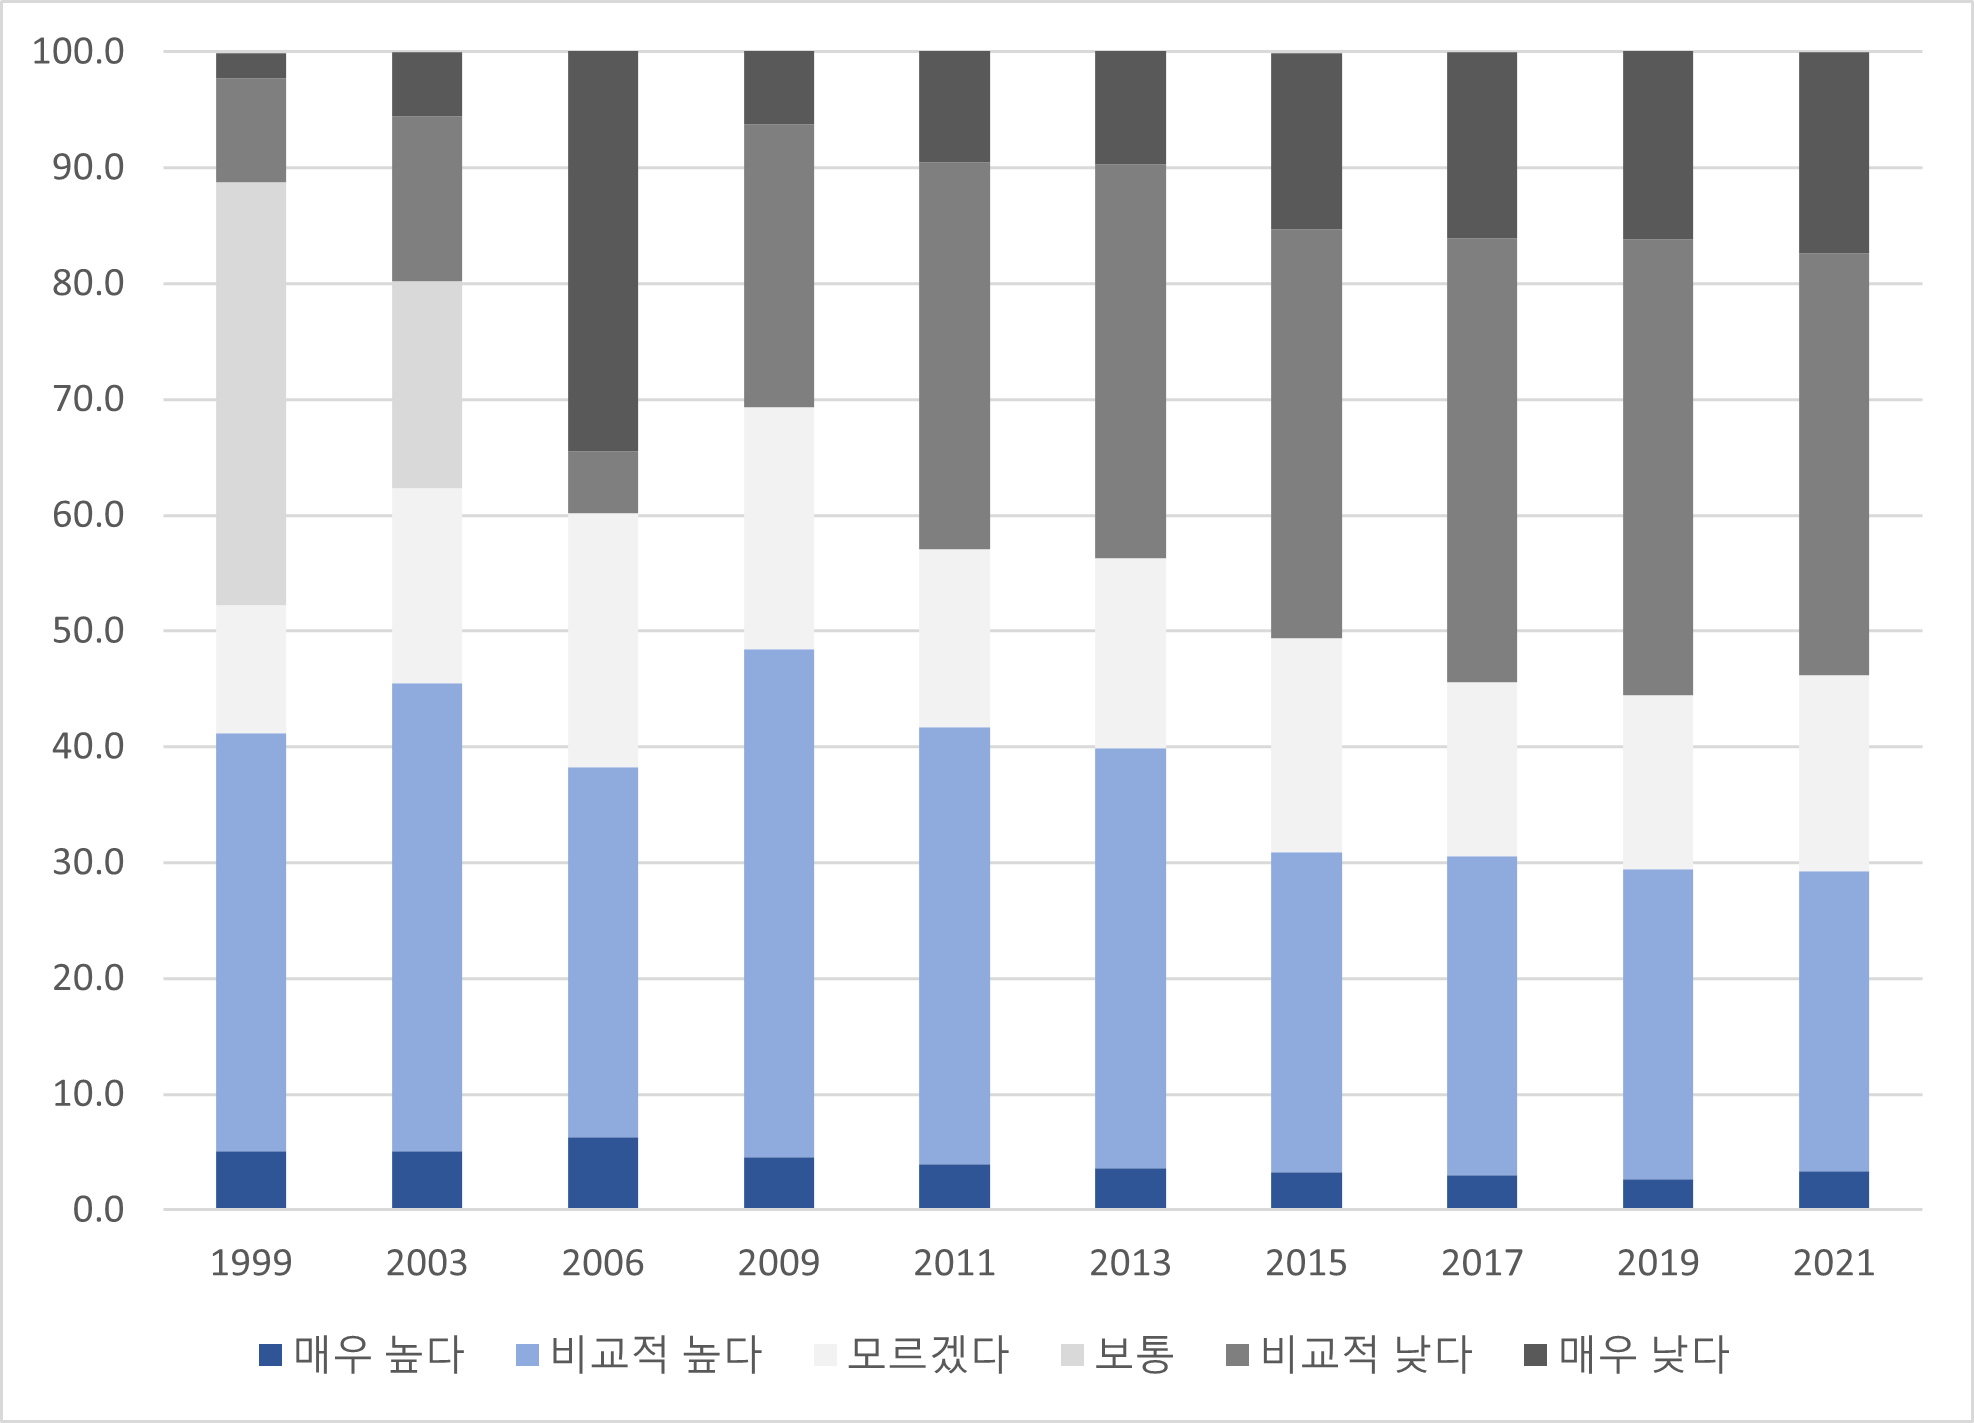
\includegraphics[width=\textwidth]{figure/kosis_intermobility_99-21.png}
        \caption{세대간 계층이동}
    \end{subfigure}
    \hfill
    \begin{subfigure}[b]{0.45\textwidth}
        \centering
        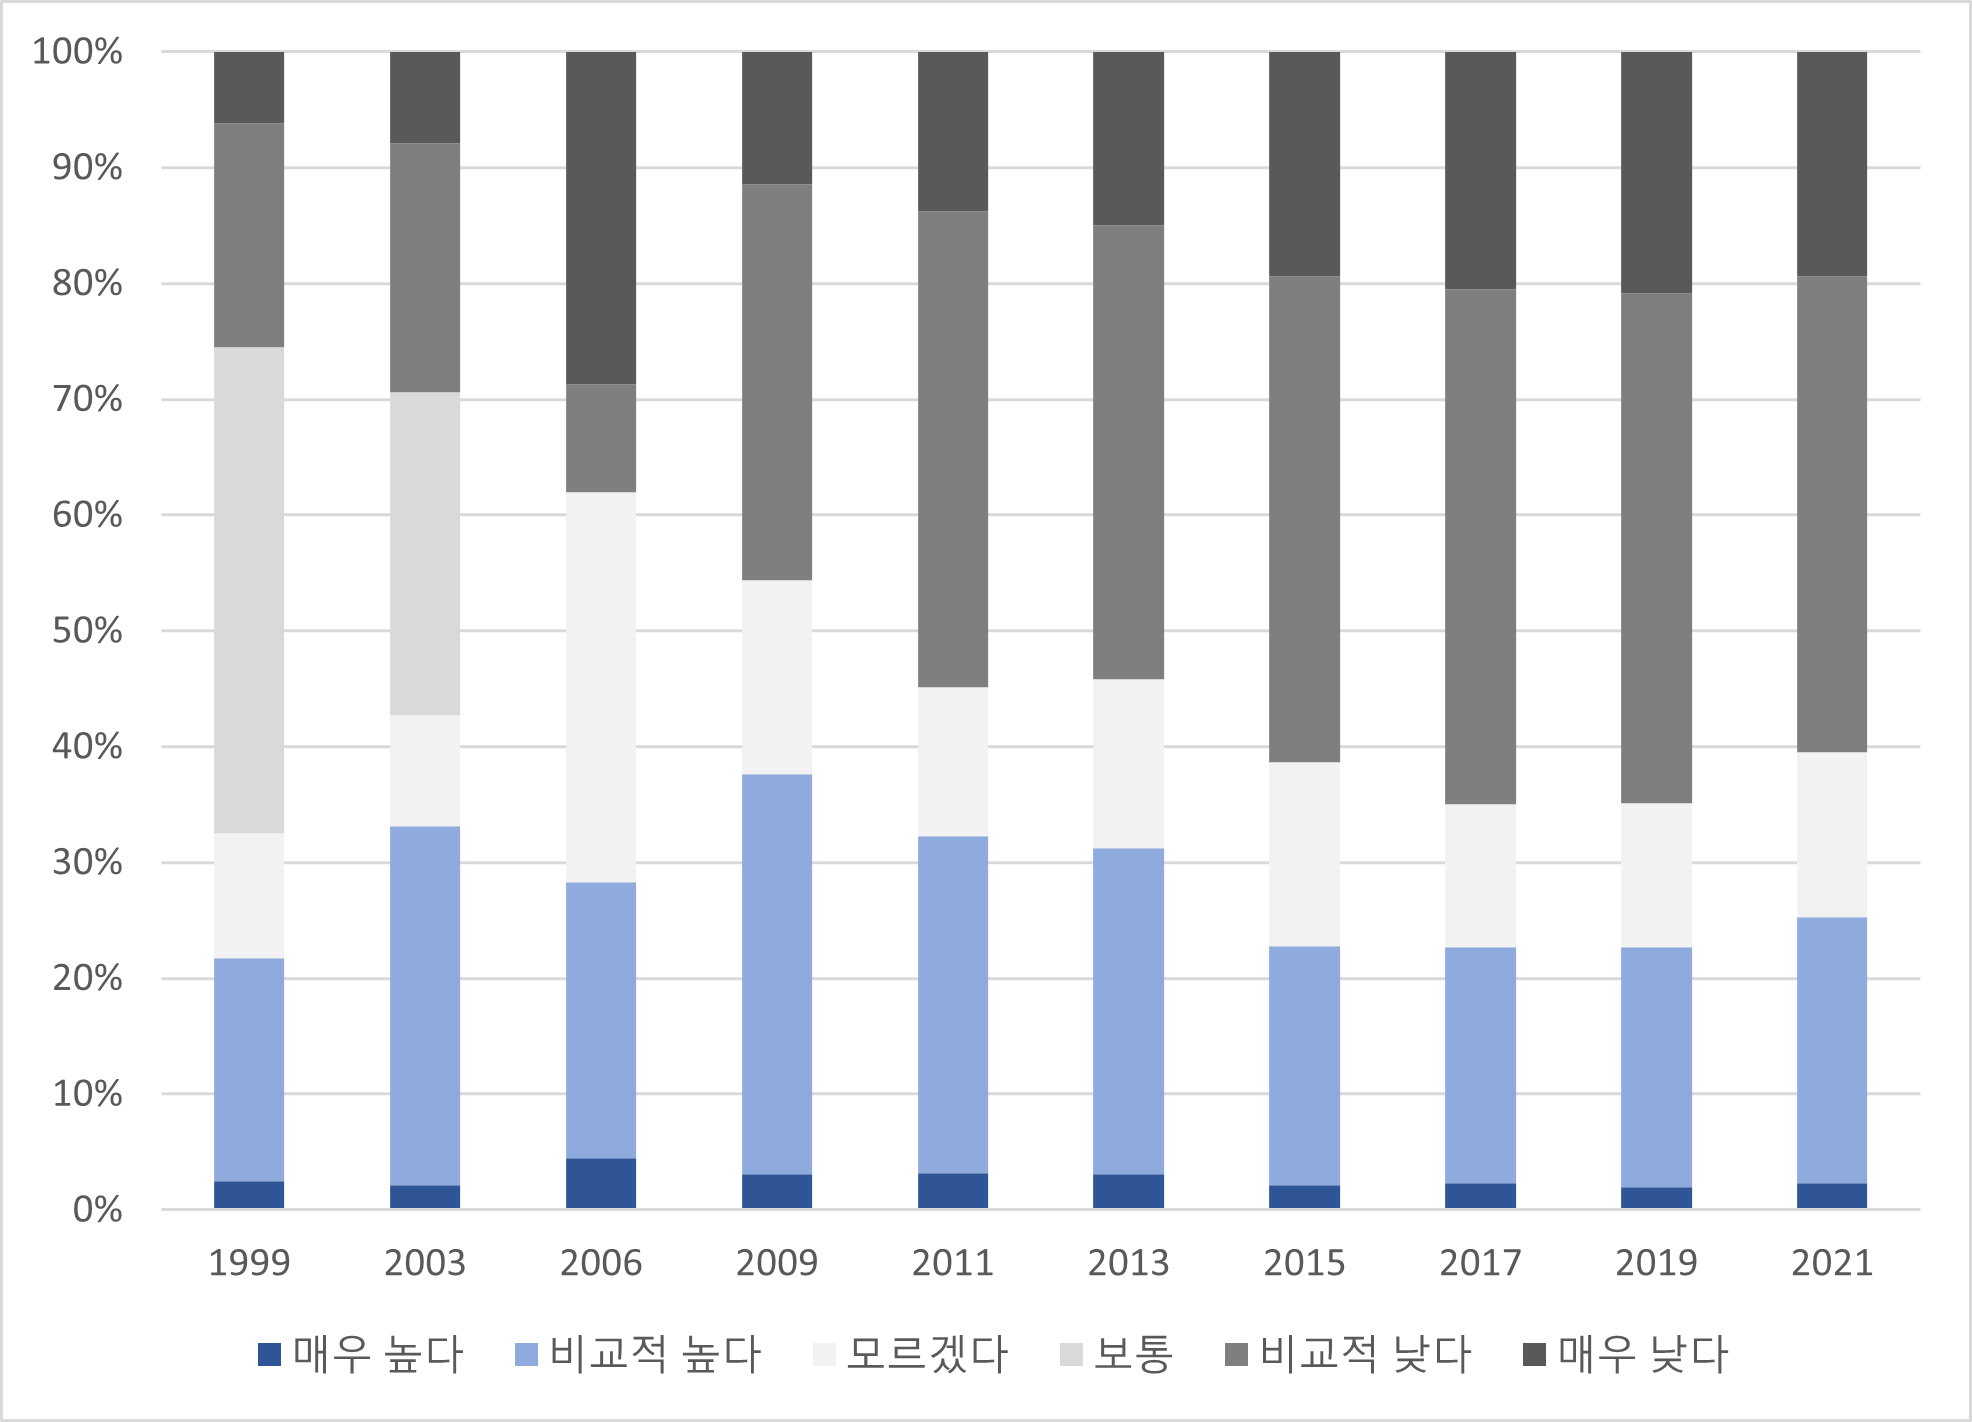
\includegraphics[width=\textwidth]{figure/kosis_intramobility_99-21.png}
        \caption{세대내 계층이동}
    \end{subfigure}
    \\
    \source{통계청, 「사회조사」, 원자료, 각 년도.}
    \label{fig:intermobility}
\end{figure}

이러한 주관적 인식의 급격한 변화와 달리 세대 간 계층이동에 대한 여러 선행연구들은 비교적 낙관적인 결론을 보였다.\footnote{한국의 지니계수 역시 2011년 0.388에서 2020년 0.331로 꾸준히 감소하여 소득분배 역시 개선되어 왔다.} \citet{cnh11}과 \citet{yang12}은 세대 간 소득탄력성(부모소득상승률에 대한 자녀소득 상승률의 비율)을 0.37이하로 추정하여 OECD국가 평균 이하었다. 이는 우리나라의 세대 간 계층이동성이 OECD 평균 보다 높은 것을 의미한다.\footnote{선행연구인 \citet{kim09}과 \citet{ketl09} 등에서는 이보다 더 낮은 탄력성이 보고되기도 하였다.}

불평등에 대한 최근의 연구는 과거와 크게 두 가지 관점에서 차이가 있다. 첫째,  불평등 연구의 대상이 부$\cdot$소득과 같은 인간행위의 결과에 머무르지 않고 이들의 주요 원인인 가정환경이나 가구소득과 같은 사회경제학적 배경을 고려한다. 다시 말해 결과의 불평등을 넘어 기회의 불평등에 초점이 맞춰지고 있다.
 
둘째, 과거에는 소득이나 부와 같은 경제적 성과에만 초점을 맞춘 불평등 문제가 대학입시제도, 특목고-자사고 축소와 같은 교육적 성취의 영역에서도 주목받고 있다. 대부분의 국가에서 교육적 성취는 개인들이 미성년기에 얻을 수 있는 가장 중요한 성취 중 하나다. 뿐만 아니라 교육적 성취는 다시 미래의 소득 획득에 중요한 요소가 된다. 따라서 교육적 성취에 대한 불평등 연구는 사회구성원이 미성년 시기에 겪는 불평등에 대한 연구와 동시에 미래의 소득불평등에 대한 원인에 대한 정보를 제공한다.

본연구의 목적은 교육과 소득이라는 생애 대표적인 두 성취에 대한 우리 사회의 기회불평등의 존재여부와 그 정도를 시계열로 제시하고 정책적 함의를 도출하는 데 있다. 우리 사회의 대다수는 성장기에 교육, 특히 대학입학를 주요 성취로 여기고 이를 달성하기 위해 매진한다. 그리고 교육과정이 끝나면 누구나 소득이나 부와 같은 경제적 성취에 매진한다. 따라서 교육 및 경제적 성취 각각을 분석함으로서 개인의 생애 전반의 성취에 대한 기회불평등 분석을 할 수 있다. 또한, 교육적 성취는 경제적 성취에 가장 중요한 설명변수다. 더 나은 교육의 성취는 두말할 나위 없이 더 나은 경제적 성취의 획득과 직결된다. 따라서 교육적 성취의 불평등에 대한 분석은 경제적 성취의 불평등을 이해하기 위해서도 중요한 자료가 된다.
 
이하의 장은 다음과 같이 구성된다.
2장에서는 대졸자직업이동경로조사(이하 GOMS)를 이용하여 2000-2011학년 고졸자의 입학대학을 성취변수로 하는 대학입학의 기회불평등과 대학졸업후 초직에서의 임금을 성취변수로 하는 경제적 기회불평등의 추이를 살펴본다. 교육적 성취의 측정에서는 수능 또는 시험점수와 같은 정량적 지표가 필요하다. 하지만 이를 공개한 전국단위의 자료는 \citet{ohetl16}에서 연구한 KEEP, KELS 두 자료가 유이하다. 그러나 두 자료는 각각 2005년 수능응시생과 2011년 수능 응시생이라는 두 코호트만을 관찰할 수 있어 교육적 성취의 기회불평등 추이를 분석할 수 없다. 반면 GOMS는 대졸자를 대상으로 조사되지만 이들의 졸업대학과 학과를 구분할 수 있어, 대학입학이라는 교육적 성취를 시계열화 하여 분석할 수 있다. 아울러 대학졸업후 초직에서 얻는 소득변수 역시 제공하여 동일한 대상에 대하여 교육적 성취와 경제적 성취를 제한적으로나마 비교분석 할 수 있다.

3장에서는 한국노동패널(이하 KLIPS)를 이용하여 1998년 이후 우리 사회 가계소득의 기회불평등 추이를 살펴본다. 2장의 자료는 대졸자를 졸업후 최장 18개월 이내에 조사하였기 때문에 경제적 기회불평등의 연구대상이 20-30대 청년으로 한정된다. 그리고 대졸자를 대상으로 하기 때문에 실제 20-30대가 겪는 실제 기회불평등보다 과소측정되는 문제가 있다. 우리 사회의 경제적 기회불평등 전체를 분석하기 위해서는 모든 개인들을 제한없이 대표하면서 소득정보 및 그들의 사회경제적 환경정보를 동시에 제공하는 자료가 필요하다. KLIPS는 이러한 조건에 부합하는 정보를 제공하여 우리 사회의 경제적 기회불평등을 시계열로 분석할 수 있게 한다.

4장에서는 연구범위와 주제를 확장한다.  주요한 두 국제 교육자료인 `수학·과학 성취도 추이변화 국제비교 연구(Trends in International Mathematics and Science Study, TIMSS)' 와 OECD 학업성취도 평가(OECD's Programme for International Student Assessment, PISA)를 이용하여 지난 20여년간 전세계 청소년의 교육성취의 기회불평등을 측정하고, 교육의 (기회)불평등이 경제성장에 어떤 영향을 주는가에 대하여 살펴본다.
5장은 이상의 연구결과에 대한 맺음글이다.

\chapter{대학입학과 청년의 경제적 성취의 기회불평등}
\section{서론}

매년 이루어지는 통계청의 사회조사에서 세대 간 계층이동성에 대한 설문에 대한 응답은 2000년대 이후 현재까지 매우 빠른 계층이동에 대한 인식의 변화를 보여준다.\footnote{본 연구는 \citet{onj20}로 출간된 바 있다.}
그러나 교육부의 2017년 설문조사에 따르면(교육부(2017), “경제⋅사회 양극화에 대응한 교육복지 정책의 방향과 과제”) 응답자의 93.9\%가 계층 간 교육격차가 크다고 응답하였고, 87\%가 과거에 비해 교육격차가 커졌다고 인식하여 계층사다리로서의 교육의 역할이 부실한 것이 세대 간 계층이동에 대한 전망의 주요 원인으로 지목되고 있다.
위 교육부 설문조사에서 교육격차의 가장 큰 원인으로 67.7\%가 교육비 격차라고 응답하였는데 실제 가계동향조사에 따르면 월 소득 600만원 이상 가정과 100만원 미만 가정의 교육비 지출 격차가 2016년 10.2배, 사교육비의 경우 12.7배에 이르는 것으로 나타났다.
대학입시와 초중등 학업성취도 자료를 이용한 여러 연구(가령, \citet{kim11}, \citet{knl08}, \citet{ketl14}, \citet{ohetl16})들이 계층 간 높은 교육격차를 보고하였고 그 원인으로 사교육비의 격차와 사교육비에 영향을 미치는 가구의 사회경제적 지위를 들고 있다.
  
계층 간 교육격차의 해소를 위해 최근 대학입시전형에서 정시 비중을 높이고 고교평준화를 강화하는 방향의 정책이 추진되고 있고 이에 대한 찬반론이 대립되고 있다.
특히 정시와 수시의 공정성 비교에 있어서 교육 및 입시 전문가들의 의견대립이 첨예하다.
본 연구는 대학입시를 둘러싸고 우리 사회의 계층 간 교육격차 혹은 교육 기회불평등의 실태를 분석하고 입시 전형 별 교육기회불평등을 비교하는 것을 목적으로 한다.
이를 바탕으로 최근 추진되고 있는 정시확대 정책의 효과에 대한 정책적 시사점을 도출할 것이다.
  
대부분의 현대 민주주의 국가에서는 인종, 성, 성장환경(부모의 사회경제적 배경, 출신지역 등), 종교 등과 같이 개인의 선택과 무관하게 타고난 환경 요인이 개인의 성취에 영향을 미쳐서는 안 된다는 기회균등의 원칙에 대한 높은 수준의 사회적 합의가 존재한다.
이처럼 기회균등이 요구되는 요인들을 (기회균등)기저요인이라 부를 것이다.
기회불평등에 대한 \citet{letl08, letl09}의 실증적 방법론에 따라, 기저요인의 정량적 크기 혹은 범주에 따라 “환경”을 구분하고 환경 별 성취도의 (조건부) 확률분포를 비교하여 확률분포 간에 제1차 (혹은 제2차) 확률지배관계가 존재할 때 기회불평등이 존재한다고 정의한다.
   
본 연구에서 고려할 기저요인은 부모의 사회경제적 배경, 출신지역, 그리고 성 이다.
각 기저요인에 따른 기회불평등의 존재 유무와 기회불평등도의 추세에 대해 분석할 것이다.
본 연구와 동일한 방법을 활용하여 교육과 소득의 기회불평등에 대해 연구한 선행연구로 \citet{letl08, letl09}, \citet{ohetl16}, \citet{onj17}, \citet{snj21} 등이 있다.
특히 \citet{ohetl16}은 대학입학수학능력평가 자료를 활용하여 가구환경 간 교육기회불평등을 연구하였다.
교육기회불평등에서 가장 중요한 교육성취가 대학입학성과라는 것은 부인하기 어려운 사실이다.
본 연구는 대학입학 성과를 바탕으로 가구환경 간 교육기회불평등을 분석한다는 점에서 차별성이 있다.
   
이 밖에 교육 혹은 소득의 계층 간 기회불평등에 대한 대다수의 선행연구들은 교육 혹은 소득의 성취에 미치는 다양한 요인들을 바탕으로 회귀모형을 설정하고 계수 추정을 통하여 가구환경, 성, 지역 등의 환경요인의 영향을 분석한다(관련 선행연구\citet{knl08} ,\citet{kim11} \citet{kim11}, \citet{ketl14} 등 참고).
이 연구들은 환경요인이 성취에 미치는 평균적 영향을 잘 보여주는 장점이 있으나 평균 이외에도 기회불평등과 관련된 성취 분포의 다른 특성들 (가령 최상위 성취의 가능성, 최하위 성취의 가능성, 성취 위험 등)에 미치는 영향까지 분석하지 않는 경우가 대부분이다.
바로 이점이 본 연구가 갖는 차별성이라 할 수 있다.
   
본 연구는 한국고용정보원의 대졸자직업이동경로(GOMS) 자료를 활용하여 2000년대 초반에서 2010년대 초반에 이르기까지의 기간 동안 매년 가구환경, 성, 지역환경 등이 고교졸업자들의 대학입학 성과 미치는 영향을 분석할 것이다.
이를 통하여 계층별, 성별, 지역별 교육기회불평등의 유무와 기회불평등도의 추세를 도출하고 정시와 수시 각 전형별 기회불평등도와 추세를 비교 검토할 것이다.
대부분의 교육자료는 종단연구(panel study) 형태로 되어 각 자료당 대학입시와 같은 교육성과는 자료조사기간 전체에 한 번 밖에 관찰되지 않는다.
따라서 교육성취와 관련된 연구의 수행에서 매년 추세를 연구할 수 없는데 본 연구가 갖는 두 번째 차별점은 여기에 있다.


\section{기회불평등과 기회불평등 지수}
개인의 성취는 자신의 노력뿐만 아니라 인종, 성, 부모의 사회경제적 지위 등과 같은 환경, 선천적인 재능 그리고 다양한 운에 따라 결정된다.
기회균등이 요구되는 환경들의 집합이 $C$로 주어져 있고 이를 기회균등기저(equal opportunity basis)라 하자.
기회균등 기저에 속한 임의의 환경 $c$에서 노력과 다른 우연적인 요인들에 따라 결정되는 성취 $y$의 확률분포 $y=F(y|c)$를 얻을 수 있다.
바로 이런 조건부 확률분포가 기회균등 기저의 모든 환경들 간에 동일해야 한다는 것으로 강한 기회평등을 정의할 수 있을 것이다.
즉 임의의 두 환경 $c,c' \in C$에 대해 $F(\cdot | c) = F(\cdot | c')$가 성립한다는 의미이다.

그러나 이처럼 강한 기회평등을 요구하는 것은 매우 비현실적이다.
서로 다른 환경이 상이한 성취의 확률분포를 가지더라도 어느 하나가 다른 하나보다 우월하지 않다면 기회평등이 침해되었다고만 볼 수는 없다.
우리는 \citet{letl08, letl09}이 제시한 보다 완화된 기회평등 개념을 활용하여 기회불평등에 대한 분석을 진행할 것이다.

\citet{letl08, letl09}의 기회평등은 어떤 환경도 그 확률분포가 다른 환경의 확률분포를 확률지배하지 않을 경우에 성립한다.
 상이한 두 환경 와 에서 개인의 성취는 각각 와 의 확률분포를 이룬다고 가정하자.
만약 성취 $y$가 취할 수 있는 모든 성취수준 $x$에 대하여, 부등식
\begin{equation}
    F(x | c) \leq F(x | c')
    \label{eq:fdom}
\end{equation}
이 성립하면 환경 $c'$에서 일정수준 이하의 낮은 성취를 이룰 확률이 다른 환경 $c$에서 보다 크다는 것을 의미한다.
 이는 성취의 전망의 관점에서 환경 $c'$이 환경 $c$보다 열악하다는 것이다.
 이처럼 모든 성취수준에서 식 (\ref{eq:fdom})이 성립하고 적어도 하나의 성취수준에서 이 부등식이 강부등식으로 성립할 때 환경 $c$가 환경 $c'$을 제1차 확률지배한다고 말한다.

만약 모든 성취수준 $x$에서, 부등식
\begin{equation}
   \int_{0}^{x} F(y | c)\,dy \leq \int_{0}^{x} F(y | c')\,dy
    \label{eq:sdom}
\end{equation}
이 성립하고 적어도 하나의 성취수준에서 이 부등식이 강부등식으로 성립할 때 환경 $c$가 다른 환경 $c$을 제2차 확률지배한다고 말한다.
이 경우 성취에 대한 위험기피적인 선호를 가진 사람은 항상 환경 $c$의 확률분포를 선호하게 된다.

기회균등기저에 속한 어떤 두 환경 간에 제1차 혹은 제2차 확률지배관계가 존재할 경우 기회불평등이 존재한다고 정의한다. 

제1차 기회불평등 조건: 어떤 두 환경 $c,c' \in C$에 대하여 $F(y | c)$와 $F(y | c')$사이에 제1차 확률지배관계가 성립한다.

제2차 기회불평등 조건: 어떤 두 환경 $c,c' \in C$에 대하여 $F(y | c)$와 $F(y | c')$사이에 제2차 확률지배관계가 성립한다.

그리고 기회평등은 이러한 기회불평등이 존재하지 않는 경우에 성립한다.
따라서 본 논문에서 기회평등한 사회는 기회균등기저에 속한 서로 다른 환경들이 상이한 성취의 기회(확률분포)를 제공할 수 있다.
단, 어느 환경도 다른 환경보다 더 확률지배적인 성취의 기회를 제공해서는 안 될 뿐이다.
 
보다 근본적으로 환경뿐만 아니라 개인의 노력도 기회불평등을 정의함에 있어서 고려되어야 한다(\citet{Roemer98}; \citet{letl08, letl09}).
즉, 동일한 노력을  한 사람들에게 환경의 기회격차가 존재해서는 안된다는 기회평등은 설득력을 가질 수 있지만 노력을 더 많이 한 사람에게 더 좋은(확률지배적) 기회가 보장되는 것을 불공정하다고 볼 수 없는 것이다.
이처럼 환경뿐만 아니라 노력의 크기까지도 조건화하여 위에서 말한 확률지배관계를 정의하고 이를 이용하여 기회불평등을 정의하는 것이 보다 근본적인 접근이라 할 수 있다.
이러한 접근법을 택하더라도 개인의 노력을 ``순수한'' 노력변수로 나타낸다면 결과적으로 앞서 정의된 노력이 고려되지 않은 기회불평등 조건이 필요조건이 될 수밖에 없다.
여기서 노력이 순수하다는 것은 노력의 분포 자체도 환경의 영향을 받지 않는다는 것을 의미한다.
이와 관련하여 보다 자세한 논의는 선행연구인 \citet{Roemer98}, \citet{letl08, letl09}, 오성재외(2016), 오성재·주병기(2017) 등에 잘 소개되어 있다.

두 기회불평등 조건에 나타난 확률지배관계 검증은 \citet{dnd00}의 비모수 검증법을 활용한다.
먼저 기회균등기저의 환경을 기준으로 집단을 나누고 환경별 성취의 누적분포함수 $F(y | c)$를 얻는다.
이렇게 얻어진 환경별 분포함수들 간에 확률지배관계 성립 여부를 검증하는 것이다.
우선 임의의 두 환경 $c,c'$사이에 $F(y | c)$가 $F(y | c')$을 1차(2차) 확률 지배를 하고 그 역은 성립하지 않을 경우 전자가 후자를 1차(2차) 확률지배하는 것으로 확인된다.
이처럼 확률지배관계가 확인되지 않을 경우 두 분포의 동일성 여부를 검증하는 순서로 진행된다.

확률지배검증은 기회불평등의 존재 유무만을 알려준다.
그러나 똑같이 기회불평등한 사회 간에도 기회불평등의 크기를 비교하려면 기회불평등 지수가 필요하다.
\citet{letl08}은 불평등 지수로 널리 쓰이는 지니계수에서 착안한 지수를 활용하였다.
환경 $t$의 평균성취수준을 $\mu _t$, 불평등도(지니계수)를 $G _t$라고 할 경우, 환경 $t$에서의 성취기회의 ``가치''는 $\mu _t (1-G _t)$로 나타낼 수 있을 것이다.
즉, 평균성취수준이 클수록 그리고 불평등도가 낮을수록 환경 $t$의 성취기회의 가치는 상승하는 것이다.
\footnote{\citet{yitzhaki79}는 $\mu _t (1-G _t)$를 환경 $t$에 속하는 개인들이 자신의 환경에 대하여 가지는 상대적 만족감이라고 한다.}
모든 환경에 대하여 이렇게 환경의 가치를 측정하고 이러한 가치 값들에 대한 불평등도를 다시 지니계수로 구한 것이 지니(Gini) 기회불평등지수(혹은, GO 지수)이다.
총 $k$개의 환경이 있고 환경 가치의 평균값을 $\mu$라고 하면, 각 환경 $t$의 비중이 $P_t$일 때, 지니 기회불평등지수는 다음 식과 같이 정의된다.

\begin{equation}
    G O=\frac{1}{\mu} \sum_{i=1}^{k} \sum_{j>i} P_{i} P_{j}\left(\mu_{j}\left(1-G_{j}\right)-\mu_{i}\left(1-G_{i}\right)\right).
    \label{eq:goms_GOI}
\end{equation}

열악한 환경에서도 최상위 성취전망이 높은 사회에서는 계층상승의 기회가 크다고 할 수 있다.
이처럼 최하위에서 최상위로의 계층상승의 전망을 반영하는 지표도 기회불평등지표로 유용하게 활용될 수 있다.
가장 열악한 환경 $\underline{c}$에 처한 사람들의 전체인구에서의 비율을 $q_{\underline{c}}$이라 하자.
최상위 성취 집단을 소득 상위 $p$퍼센트에 속하는 사람들이라고 하고 이들의 수를 $n_p$라고 하자.
 
그리고 이들 중 가장 열악한 환경 $\underline{c}$에 처한 사람들의 $n_{p,\underline{c}}$수를 라고 하면, 개천용(기회)불평등지수(혹은, RR 지수)는 최상위 성취집단에서 최하위 환경의 비율을 이용하여 다음과 같이 정의된다
\footnote{개천용불평등지수는 본 연구와 동시에 진행된 교육기회불평등에 대한 연구인 오성재外(2017)에서도 소개된 바 있다.}
\begin{equation}
    R R_{p}=1-\frac{n_{p, \underline{c}} / n_{p}}{q_{\underline{\underline{c}}}} .
    \label{eq:goms_RRI}
\end{equation}
개천용불평등지수 값이 0이라는 것은 최상위 성취를 이룬 사람들 중에서 최하위 환경을 가진 사람들의 비율이 최하위 환경 사람들의 인구비율과 동일하다는 것을 의미하고 이는 기회불평등이 없는 상태를 나타낸다.
 개천용불평등지수 값이 1이라는 것은 반대로 최상위 성취를 이룬 사람들 중에서 최하위 환경을 가진 사람이 없다는 것을 의미하고 이는 기회불평등도가 가장 높은 상태를 나타낸다.
 개천용불평등지수 값이 음이 되는 경우도 있는데 이는 최하위 환경이 최상위 성취를 달성하는데 오히려 유리한 ``역''기회불평등의 상태를 말한다.

개천용불평등지수가 0인 사회에서는 가장 열악한 환경에서도 다른 환경과 동일한 확률로 성공이 보장된다고 볼 수 있다.
개천용불평등지수가 양수 의 값을 가진다면 최악의 환경에서 성공할 수 있는 100명 중에서 $100 \times q$명(퍼센트)가 기회불평등 때문에 성공하지 못하는 것으로 볼 수 있다.
예를 들어 개천용불평등지수가 0.6인 사회에서는 최악의 환경에서 성공할 수 있는 100명중에서 60명이 기회불평등 때문에 실패하게 되는 것이다.
\footnote{본 연구에서는 성공의 기준을 최상위 등급의 대학진학으로 정의한다.}


\section{분석자료}
대졸자직업이동경로조사(이하 GOMS)는 한국고용정보원 주관으로 2005년부터 집계된 반복 횡단면 자료이다.
목표 모집단은 조사시점 최근 1년간 전국의 모든 대학졸업자이고 이 가운데 약 4\%에 해당하는 18,000명을 조사하고 있다.
 (비)경제활동상황, 일자리상태, 학교생활, 취업준비, 인적사항 등의 정보를 수집하고 있다.
 최초구상은 2005년부터 조사하는 종단면 자료로 계획되었으나, 예산문제로 2006년 조사가 시행되지 못했다.
 2007년부터 매 해 1차 조사 및 2년 후 1회 추적조사를 실시하는 것으로 변경되었고, 2012년부터는 매 해 1차 조사만 시행하고 있다.
 본 연구는 2007년부터 2017년까지의 1차 조사 자료를 반복된 횡단면 자료로 활용하였다.

\begin{figure}
    \centering
    \caption{고교졸업년도별 관측치}
    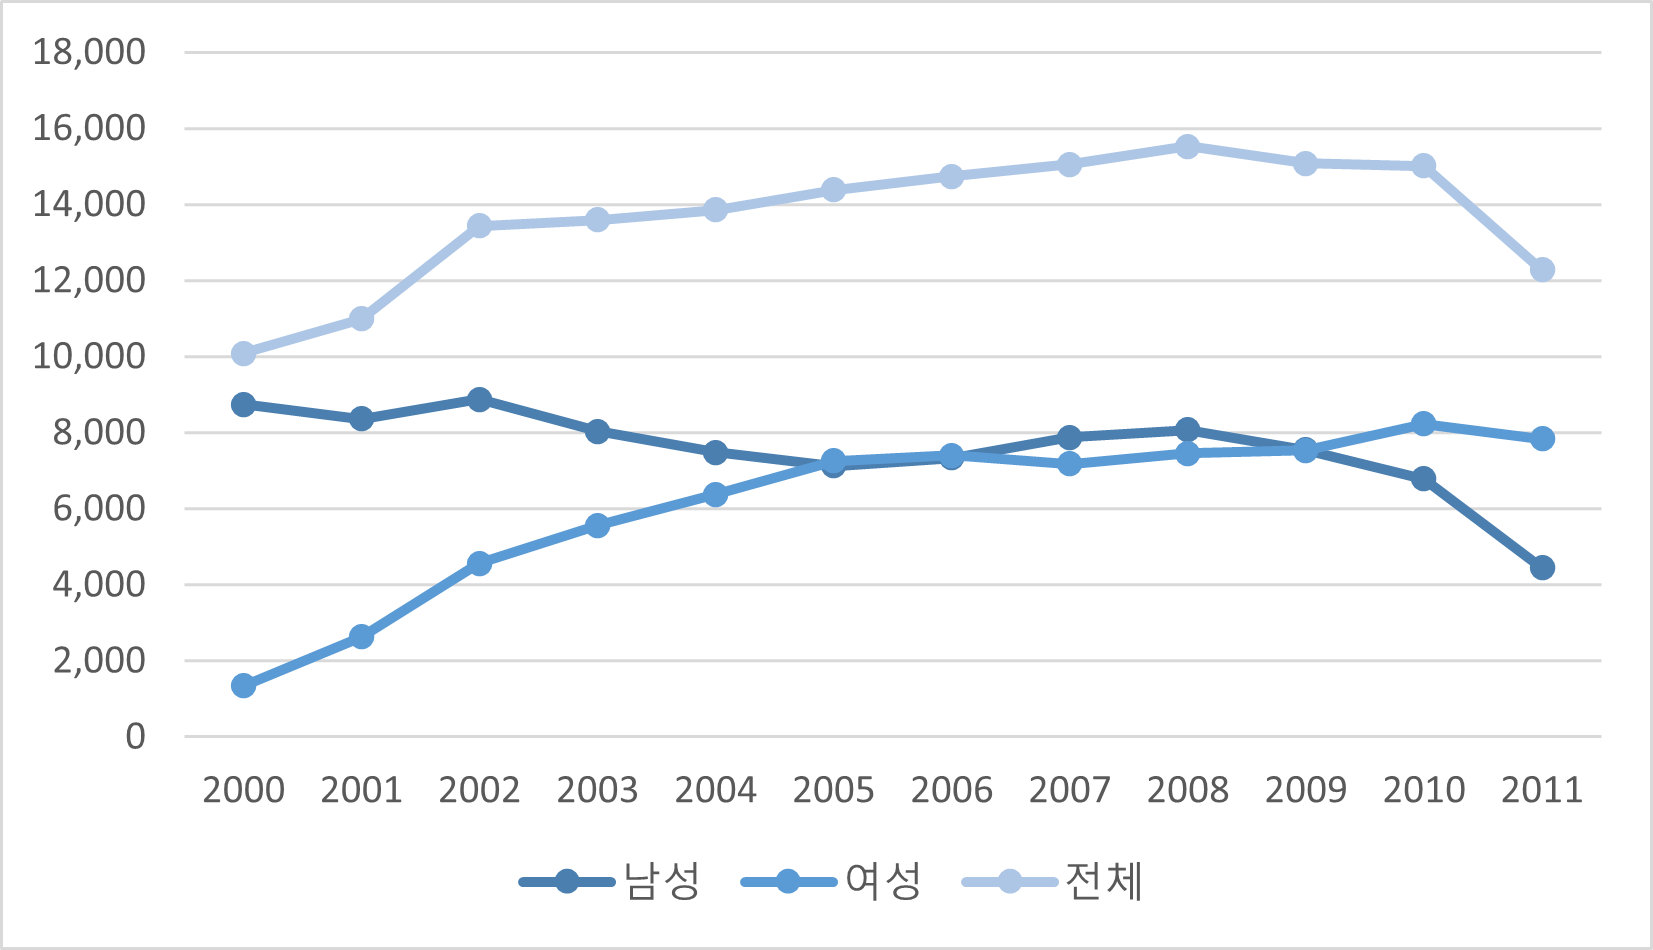
\includegraphics[width=\textwidth]{figure/goms_gender.png}
    \label{fig:goms_gender}
\end{figure}

GOMS의 모집단은 최근 1년 이내의 대학 졸업자들이다.
이들을 고교졸업년도를 기준으로 2000년에서 2011년까지 총 12개 코호트로 분류하였다.
 1999년 이전과 2012년 이후의 경우 코호트 집단의 학생 수가 크게 줄어들어 분석에서 제외하였다(그림 \ref{fig:goms_gender}참조).

군 복무 문제로 남학생과 여학생의 성비가 자료의 초기와 말기에 큰 불균형이 발생하는 것을 피하기 어렵다.
또한 자료의 초기에는 대학교육 연수가 평균보다 긴 학생들이 더 많은 비중을 차지하고 말기에는 반대로 이런 학생들의 비중이 줄어드는 문제도 존재한다는 것을 염두에 둘 필요가 있다.
대체로 성비 균형을 보이는 코호트는 2004년에서 2009년까지이다.
2004년 이전 코호트에는 여성이 과소 집계되었고 2010년 이후에는 남성이 과소 집계되었다.
그러나 성별 기회불평등이 미미하다는 점을 고려할 때 이러한 성비의 문제는 분석에 큰 영향이 없을 것이라 짐작한다.

교육성취는 졸업자들의 졸업대학 및 전공 정보와 2019년 QS 대학순위를 결합하여 1점에서 5점까지로 점수화하였다.
먼저 QS순위기준 최상위 대학 및 전국의 의, 치, 한, 수의대 및 약대에 5점을 부여하였다. 다음으로 QS순위 최상위를 제외환 10위까지의 대학은 4점, QS 순위 11-49위 및 전국의 교육대학은 3점, 그 밖의 4년제 대학은 2점, 그리고 2-3년제 대학은 1점을 부여하였다. 

기회균등기저에는 부친 및 모친의 학력과 부모의 대학입학당시 소득, 성, 그리고 출신고교의 소재지와 같은 환경변수를 포함시켰다.
또한 부모 학력과 소득을 이용한 주성분분석에서 얻어진 가구환경지수를 환경변수로 포함하였다. 
부친의 학력과 모친의 학력은 무학에서 대학원까지 7개로 각각 분류되어 있는데 이를 단순 합하여 2-14까지 범주로 구성하였고 이를 코호트별로 3등분에 가깝게 저, 중, 고 세 수준으로 나눠 기회불평등에 대한 분석을 진행하였다. 
부모의 소득은 8개 문항으로 조사되었는데 최저가 월소득 100만원 미만이고 최고가 월소득 1000만원 이상이다.
문항의 결과를 부모교육환경과 마찬가지로 코호트 기준 3등분에 가깝게 저, 중, 고 세 수준으로 나눴다. 
부모의 소득은 주로 중위가 많고 학력의 경우 고졸의 수가 전체에서 차지하는 비중이 높다.
이에 더해 소득은 경제성장에 의해 매년 상승하고, 과거 교육기회의 확대에 의해 매년 학부모의 교육수준 역시 급격하게 상승한다.
따라서 이를 코호트별로 세 집단으로 분할할 경우 각 집단의 비율을 동일하게 유지하기 어렵다.
이 뿐만 아니라 고교생의 교육적 성취에 영향을 미치는 성장가구의 환경변수를 얻는데 부모의 학력과 소득를 모두를 집계하는 것이 보다 적절하다 할 수 있다.
따라서 부모의 학력과 소득을 주성분분석(Principal Component Analysis)을 통해 단일변수로 집계하였고 집계된 가구환경지수 값의 분포를 3등분에 가깝게 저, 중, 고 세 가구환경으로 나눴다.
 
성장지역환경은 출신고교의 소재지를 기준으로 서울, 경기 일부지역 및 인천을 수도권, 나머지 광역시 및 세종시를 광역시권, 수도권 이외의 경기도 지역과 나머지 도 단위 및 제주도를 도지역권으로 나눴다.
\footnote{서울과 인접하고 인구가 많은 고양시, 광명시, 부천시, 성남시, 수원시, 안산시, 안양시, 용인시, 의정부시를 수도권에 포함했다.}

 한국의 자료를 이용한 기회불평등 분석에서 환경유형의 구분은 주의해야 한다. 우리 사회는 60년대 이후 산업구조와 교육기회 양자에서 급격한 진보를 경험했다. 그 결과 개인들의 부모의 학력 또는 직업력을 이용해 환경유형을 구분할 경우, 그 구성비가 시계열적으로 계속 변화한다.
 <그림 \ref{fig:goms_nratio_byedu}>은 각 코호트별 부친의 학력을 기준으로 할 경우의 구성비다.
  2000년 코호트는 초대졸 이상이 31.79\%인데 이 비율은 졸업년별로 지속적으로 증가하여 2011년 코호트는 46.80\%가 초대졸이상의 학력을 가진 부친을 두게 된다.
 \footnote{조사대상의 부모가 대학을 입학했던 시점인 1981년을 기준으로 정부 정책에 의해 대학교 신입생 정원이 1년만에 20만명대에서 30만명대로 10만명 가량 증가하였다.}
고졸부친은 전체 코호트에서 44\% 근처로 일정하지만 초대졸 이상의 비율이 늘어나는 만큼 중졸이하의 비중이 15\% 가량 줄어든다. 따라서 부모의 학력을 기준으로 환경을 세 가지 유형으로 분리할 경우 코호트별로 환경유형의 구성이 계속 바뀐다.
c
\begin{figure}
    \centering
    \caption{부친학력기준 자료비율}
    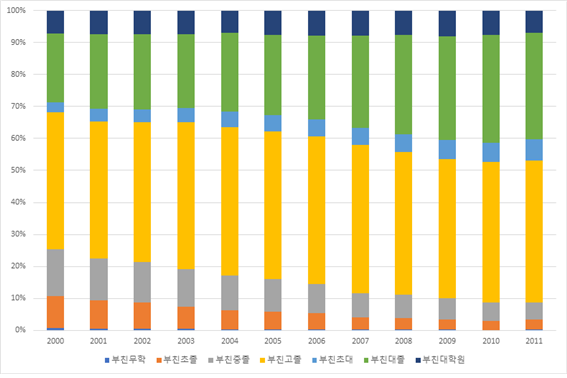
\includegraphics[width=\textwidth]{figure/goms_nratio_byedu.png}
    \label{fig:goms_nratio_byedu}
\end{figure}

이 문제는 주성분 분석(Principal Component Analysis) 기법을 통해 해결하였다.
<그림 \ref{fig:goms_pca}>의 오른쪽은 부친의 학력, 모친의 학력, 부모의 소득 세 변수를 설명변수로 하는 주성분점수의 값의 코호트별 분포이다.
 <그림 \ref{fig:goms_nratio_byedu}>과 같이 범주화된 점수와 비교했을 때, 개인에게 할당된 주성분 점수는 상당히 연속적임을 알 수 있다.
 <그림 \ref{fig:goms_pca}>의 왼쪽은 코호트별로 주성분 점수를 3등분 하여 저, 중, 고유형으로 범주화 한 비율의 히스토그램이다.
 점선은 $1/3$ 값인데 코호트별로 환경유형이 고르게 분할되었음을 알 수 있다.

\begin{figure}
    \centering
    \caption{코호트별 주성분점수(우)와 주성분분석환경 구성비율(좌)}
    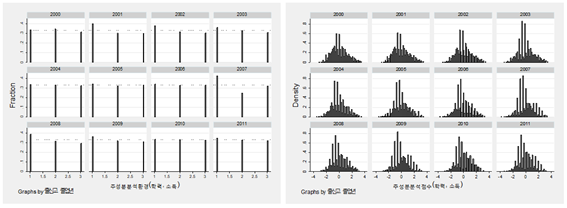
\includegraphics[width=\textwidth]{figure/goms_pca.png}
    \label{fig:goms_pca}
\end{figure}

어떤 대학입시 유형이 공정한가는 교육의 기회와 관련하여 최근 주목받는 주제이다.
이를 분석하기 위해 본 자료에서 제공되는 개인들이 응시한 대입유형 변수를 활용하여 일반 정시, 일반 수시, 특별전형 및 기타로 나누었다.
 일반 정시는 정시, 수능 위주, 논술 위주 및 실기 위주 입시를 포함하고 일반 수시는 수시, 학생부종합 및 학생부교과 위주의 전형을 포함한다.
 특별전형 및 기타는 수시, 정시와 관계없이 정원외 정원 등의 특별전형을 포함하는데 이들은 입시유형별 분석에서는 제외하였다.

\begin{table}[htbp]
    \centering
    \caption{학년도별 대입정원의 정시$\cdot$수시 구성}
    \resizebox{\textwidth}{!}{
\begin{tabular}{c|c|c|c|c|c|c|c}
\hline 학년 & 수시 $^{*}$ & 수시비율 $^{*}$ & 정시 $^{*}$ & 정시비율 $^{*}$ & 합계 $^{*}$ & 수시비율 & 정시비율 \\
\hline 2002 & 107,821 & $28.8 \%$ & 266,063 & $71.2 \%$ & 373,884 & $12.6 \%$ & $81.5 \%$ \\
\hline 2003 & 112,667 & $29.3 \%$ & 271,359 & $70.7 \%$ & 384,026 & $17.1 \%$ & $78.1 \%$ \\
\hline 2004 & 155,941 & $38.5 \%$ & 248,995 & $61.5 \%$ & 404,936 & $24.1 \%$ & $71.1 \%$ \\
\hline 2005 & 174,979 & $44.4 \%$ & 219,400 & $55.6 \%$ & 394,379 & $29.7 \%$ & $65.6 \%$ \\
\hline 2006 & 188,213 & $48.3 \%$ & 201,371 & $51.7 \%$ & 389,584 & $32.0 \%$ & $63.6 \%$ \\
\hline 2007 & 194,442 & $51.5 \%$ & 183,021 & $48.5 \%$ & 377,463 & $34.5 \%$ & $60.3 \%$ \\
\hline 2008 & 200,878 & $53.1 \%$ & 177,390 & $46.9 \%$ & 378,268 & $35.4 \%$ & $58.8 \%$ \\
\hline 2009 & 214,481 & $56.7 \%$ & 163,996 & $43.3 \%$ & 378,477 & $34.8 \%$ & $58.2 \%$ \\
\hline 2010 & 219,024 & $57.9 \%$ & 159,117 & $42.1 \%$ & 378,141 & $34.9 \%$ & $56.8 \%$ \\
\hline 2011 & 232,781 & $60.7 \%$ & 150,761 & $39.3 \%$ & 383,542 & $37.9 \%$ & $52.6 \%$ \\
\hline
\end{tabular}}
    \source{별표(*)는 대학교육협의회, 나머지는 GOMS 자료.}
    \confer{2001년 이전은 대입특차전형(수능 100\% 선발) 제도가 존재.}
    \label{tab:goms_enttype}
\end{table}

<표 \ref{tab:goms_enttype}>은 대학교육협의회에서 발표하는 학년별 정시 및 수시 신입생 모집인원에 대한 자료와 GOMS 자료를 통해 살펴본 정시와 수시로 대학을 입학하여 졸업한 개인들의 비율이다.
특별히 흥미로운 점은 정시의 비율이 모집정원보다 졸업생이 10-15\%p 정도 꾸준히 높다는 점이다.
교육통계연보에 따르면 매년 대학 신입생의 약 20\%가 재수생인데 이들 재수생은 상당수가 수시전형으로 기합격한 대학생일 것으로 짐작캐 한다.

본 연구에서 코호트 선정은 모집단과 연구주제의 불일치 문제로 복잡하다.
GOMS의 모집단은 최근 1년 이내 대졸자인데 이들의 동질성은 노동시장 분석에 적합하고, 교육성취의 관점에서 이들은 상이한 나이 및 초중등교육과정을 거쳤기 때문에 코호트로서 부적절하다.
 코호트 선정에 활용할 수 있는 정보는 출생연도, 고교졸업 연도, 대학입학 연도 세 가지가 있다.
 이 가운데 대학입학의 최소 요건이 충족되는 고교졸업 연도를 기준으로 삼는다.
 고교졸업 년은 1955년에서 2015년까지 다양한데, 자료조사가 2007년부터 2017년까지 총 11개 시점에서 이루어진 점을 고려하여 가장 빈도가 높은 11개 고교졸업 년을 대상으로 한다.
 
 소득에 대한 분석에서는 개인들의 다양한 직업지위을 고려해야 한다.
 자료에서 직업지위를 파악할 수 있는 변수로 i) 소속 기업체의 규모, ii) 고용행태, iii) 근로계약서상 계약 기간 명시 여부, iv) 스스로 생각하는 정규직 여부 등이 있다.
  우리는 이를 자영업자, 비정규 직근로자, 정규근로자의 세 가지 분류로 나눈다.
  정규직 근로자는 100인 이상 고용 기업에 다니면서, i) 근로기간이 정해지지 않은 상용근로자이거나 ii) 스스로 정규직이라고 인정하는 근로자다.
  그 밖에 임시직 및 일용직 근로자 이거나 100인 미만 기업체 근로자는 모두 임시근로자으로 분류하였다.
  마지막으로 자영업자는 고용인원에 상관없이 동일한 자영업자로 분류했다.
  <표 12>은 이러한 기준으로 정한 코호트별 정규직, 임시직, 자영업자의 수와 비율을 나타내었다.
 
\begin{table}[htbp]
    \centering
    \caption{고교졸업년별 직업지위 현황}
    \resizebox{\textwidth}{!}{
\begin{tabular}{c|c|c|c|c|c|c|c}
\hline 고교졸업년 & 자영업 (명) & 임시근로자 (명) & 정규근로자 (명) & 미취업 (명) & 정규직$\cdot$자영업 & 취업률 & 합계(명) \\
\hline 2000 & 326 & 3,924 & 3,694 & 2,143 & $39.85 \%$ & $78.75 \%$ & 10,087 \\
\hline 2001 & 353 & 4,420 & 3,734 & 2,483 & $37.19 \%$ & $77.41 \%$ & 10,990 \\
\hline 2002 & 380 & 5,764 & 4,304 & 2,992 & $34.85 \%$ & $77.74 \%$ & 13,440 \\
\hline 2003 & 424 & 5,987 & 3,988 & 3,202 & $32.44 \%$ & $76.46 \%$ & 13,601 \\
\hline 2004 & 372 & 6,270 & 3,956 & 3,259 & $31.23 \%$ & $76.48 \%$ & 13,857 \\
\hline 2005 & 400 & 6,573 & 3,920 & 3,494 & $30.03 \%$ & $75.71 \%$ & 14,387 \\
\hline 2006 & 422 & 6,535 & 4,132 & 3,653 & $30.89 \%$ & $75.22 \%$ & 14,742 \\
\hline 2007 & 393 & 6,481 & 4,264 & 3,915 & $30.94 \%$ & $73.99 \%$ & 15,053 \\
\hline 2008 & 386 & 6,781 & 4,313 & 4,051 & $30.26 \%$ & $73.92 \%$ & 15,531 \\
\hline 2009 & 332 & 6,427 & 4,094 & 4,223 & $29.36 \%$ & $71.99 \%$ & 15,076 \\
\hline 2010 & 287 & 6,565 & 4,037 & 4,123 & $28.80 \%$ & $72.54 \%$ & 15,012 \\
\hline 2011 & 232 & 5,541 & 2,992 & 3,514 & $26.26 \%$ & $71.38 \%$ & 12,279 \\
\hline 합계/평균(\%) & 4,307 & 71,268 & 47,428 & 41,052 & $31.54 \%$ & $74.98 \%$ & 164,055 \\
\hline
\end{tabular}}
    \label{tab:goms_job_byyear}
\end{table}
 
 소득분석은 모든 취업자와와 정규근로자$\cdot$자영업자만을 별도의 기준으로 하여 각각 분석하였다.
 먼저 모든 졸업자를 대상으로 하는 분석을 통해 개인들의 대학졸업 이후 일정한 시점에서 소득성취의 기회불평등을 평가할 수 있다.
  하지만 미취업자나 임시근로자는 미래에 직업이 바뀔 가능성이 크다.
  미취업자의 경우 절대다수가 취업준비를 하고 있고, 비정규직은 최대 2년안에 이직을 할 것이다.
  반면, 정규직의 경우 장기간 현직을 유지할 가능성이 크다.
  자영업자도 스스로의 의지로 직업을 유지하기 위해 최선을 다 할것이므로 이들에 대한 기회불평등 분석은 우리 사회의 미래 소득의 기회불평등을 전망하는데 더 적합하다.
 
\begin{figure}
    \centering
    \caption{직업지위별 소득의 누적분포}
    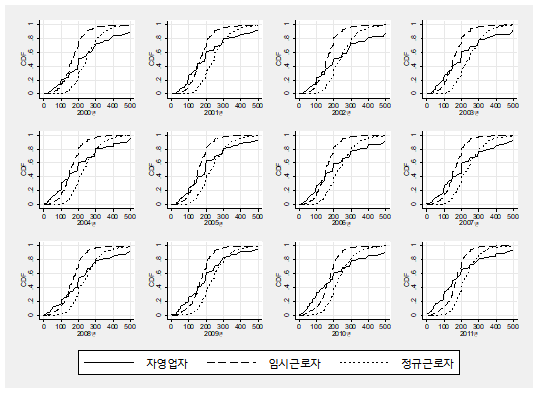
\includegraphics[width=\textwidth]{figure/goms_cdf_myjob.png}
    \label{fig:goms_cdf_myjob}
\end{figure}

 <그림 \ref{fig:goms_cdf_myjob}>은 각각의 코호트에서 직업지위별 소득의 누적분포를 그린 그림이다.
 임시근로자와 정규근로자의 누적분포는 서로 교차없이 정규근로자의 분포가 우하단에 위치하여 임의의 소득을 기준으로 정규근로자가 임시근로자에 대하여 우위에 있다.
  자영업자의 분포를 살펴보면 150만원 이하의 소득에서는 임시근로자보다  좌상단에 있어 불리한 반면 300만원 이상의 소득에서는 정규근로자보다 우하단에 오히려 유리한 모습을 보였다.
 
\section{대학입학의 기회불평등}
먼저 대학입학의 기회불평등 분석결과를 제시한다.
개별 코호트에서 환경유형별 누적분포를 제시하여 개별 환경유형이 획득한 성취의 대략적인 형태를 살펴본다.
 이어서 확률지배검증을 통해 기회불평등의 존재여부를 판단한다.
 지니기회불평등지수를 통해 전반적인 기회불평등 정도의 추이를 살펴보고, 이를 성별 및 입시유형별로 나누어 계산한 값을 통해 소집단에서 집단내 기회불평등의 형태도 아울러 살펴본다.
 마지막으로 개천용불평등지수를 이용하여, 불리한 환경에 속한 개인들이 뛰어난 성취를 획득하는데 있어 기회불평등의 정도를 살펴본다.

\subsection{누적분포함수}
누적분포함수는 총 네 가지 환경 가운데 주성분분석환경과 출신고교지역 두 가지만 제시한다.
\footnote{부모소득환경 및 부모학력환경은 주성분분석환경과 유사한 형태의 분포를 보여 별도로 제시하지 않는다.}
그림 (\ref{fig:goms_cdf_bypca})은 분석 기간인 2000년에서 2011년에 걸쳐 연도별로 가구환경 조건부 대학입학성과의 누적분포를 나타낸 것이다.
주성분분석환경의 누적확률분포는 열악한 환경이 좌상단에 위치하고 유리한 환경이 우하단에 위치하여 전형적인 기회불평등 상황에 놓여있음을 알 수 있다. 

\begin{figure}
    \centering
    \caption{가구환경별 교육성취의 누적분포}
    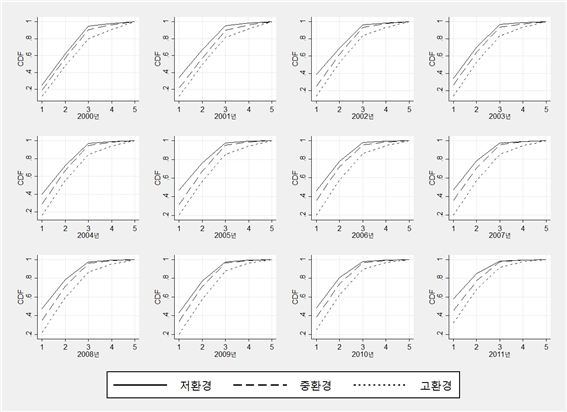
\includegraphics[width=\textwidth]{figure/goms_cdf_bypca.png}
    \label{fig:goms_cdf_bypca}
\end{figure}

출신고교가 위치한 지역에 따른 기회불평등을 확인하기 위해 출신지역을 앞서 설명했던 것처럼 수도권, 광역시, 시군구, 세 가지로 나누고 각 지역구분 별 대학입학성과의 누적분포함수를 도출하여 나타내면 그림 (\ref{fig:goms_cdf_byrgn})와 같다.
출신고교지역 환경에서는 유리한 환경으로 생각한 수도권이 왼쪽 위에 위치하는 경우가 많고 각 환경유형별 함수가 밀접하게 붙어있거나 교차하여 기회불평등이 거의 없는 상황임을 알 수 있다. 

\begin{figure}
    \centering
    \caption{출신지역별 교육성취의 누적분포}
    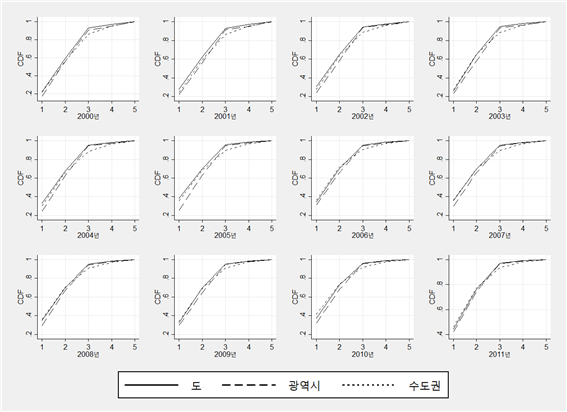
\includegraphics[width=\textwidth]{figure/goms_cdf_byrgn.png}
    \label{fig:goms_cdf_byrgn}
\end{figure}

대학입학에 있어서 성별 기회불평등을 살펴보기 위하여 남성과 여성의 교육성취 누적분포함수를 도출하여 <그림 \ref{fig:goms_cdf_bysex}>에 나타내었다.
남녀의 성비가 어느 정도 균형을 가진 2005년에서 2009년까지의 누적분포함수들을 비교할 때, 모든 연도에서 남성의 누적분포가 여성의 누적분포를 확률지배하여 성별 기회불평등이 존재하는 것으로 나타난다.
 그러나 그 격차는 가구환경별 누적분포의 격차에 비해 뚜렷하지는 않다. 특히 4-5점의 상위권 대학 진학률에서 격차가 작은 것을 알 수 있다.
 
\begin{figure}
    \centering
    \caption{성별 교육성취의 누적분포}
    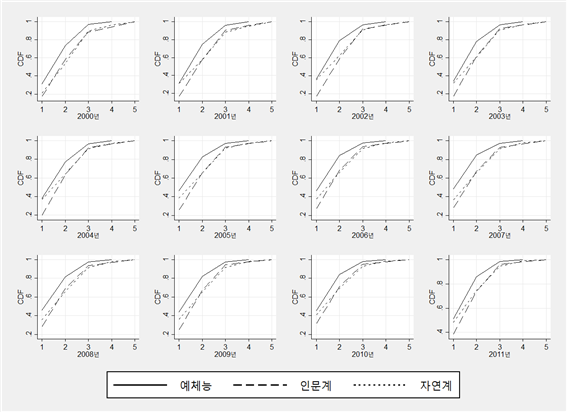
\includegraphics[width=\textwidth]{figure/goms_cdf_bysex.png}
    \label{fig:goms_cdf_bysex}
\end{figure}

마지막으로 대학계열별 교육기회불평등의 존재 유무를 살펴보기 위하여 계열별로 대학입학 성과의 누적분포를 도출하여 <그림 \ref{fig:goms_cdf_byfld}>에 나타내었다.
예체능계의 경우 대학의 선택의 폭이 협소하여 다른 계열에 비해 대학입학 성과가 낮을 것으로 예상된다.
 실제 이런 예상과 같이 예체능계를 선택할 때 대학입학 성과의 누적분포는 인문계 및 자연계에 비해 확연히 열등한 것으로 나타났다.
 그러나 예체능계의 경우 인문, 자연계와 다르게 학교의 종합적인 순위로 성취수준을 정하는 본 연구의 방법이 학생들의 성취에 대한 객관적인 척도라 할 수 없을 것이다.
 \footnote{ 예를들어 연세대, 고려대 본교에는 미술, 체육계열 단과대가 없고 사범대학에 해당계열 학과가 있다.}
 인문계와 자연계 간에는 대학입학 성과의 누적분포 간에 우열관계는 없는 것으로 보이고 두 누적분포가 거의 구분되지 않는 것으로 나타난다.
 
\begin{figure}
    \centering
    \caption{대학계열별 교육성취의 누적분포}
    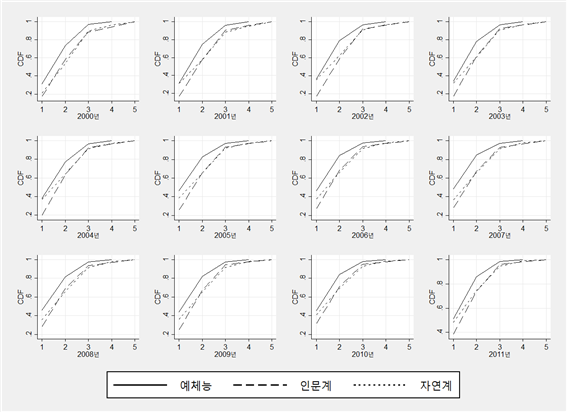
\includegraphics[width=\textwidth]{figure/goms_cdf_byfld.png}
    \label{fig:goms_cdf_byfld}
\end{figure}

\subsection{확률지배결과}

주성분분석 환경하에 확률지배검증 결과 거의 모든 코호트에서 환경유형간에 기회불평등이 존재하는 상황을 확인했다.
특히 대부분의 경우에서 1차 확률지배가 존재하여, 우월한 환경에 속한 수험생들이 평균적으로 좋은 대학에 진학 했음을 알 수 있다.
흥미롭게도 지역의 경우 도 지역과 광역시 사이에서만 일관된 기회불평등이 관찰되는 반면 수도권은 도 지역에 대해서 불분명한 관계인 경우가 많았다.
 광역시와의 비교에서는 오히려 수도권이 확률지배 당하여 이들이 기회불평등 한 경우가 많았는데, 이는 인구가 많은 지역에서 소득 격차가 큰 현상처럼 수도권 학생들의 교육성취 편차가 큰 탓이라고 생각할 수 있다.
 
\begin{table}[htbp]
    \centering
    \caption{PCA환경하 대학입학성과 누적분포의 확률지배 검증결과}
    \begin{tabular}{c|c|c|c|c|c|c}
\hline & \multicolumn{3}{|c|}{중환경} & \multicolumn{3}{c}{고환경} \\
\hline \multirow{4}{*}{저환경} & $<_{1}^{* * *}$ & $<_{1}^{* * *}$ & $<_{1}^{* * *}$ & $<_{1}^{* * *}$ & $<_{1}^{* * *}$ & $<_{1}^{* * *}$ \\
\cline{2-7} & $<_{1}^{* * *}$ & $<_{1}^{* *}$ & $<_{1}^{* * *}$ & $<_{1}^{* * *}$ & $<_{1}^{* * *}$ & $<_{1}^{* * *}$ \\
\cline{2-7} & $<_{1}^{* * *}$ & $<_{1}^{* *}$ & $<_{1}^{* * *}$ & $<_{1 }^{* * *}$ & $<_{1 }^{* * *}$ & $<_{1 }^{* * *}$ \\
\cline{2-7} & $<_{2}^{* * *}$ & $<_{1}^{* * *}$ & $<_{2}^{* * *}$ & $<_{1}^{* * *}$ & $<_{1}^{* * *}$ & $<_{1}^{* * *}$ \\
\hline \multirow{4}{*}{중환경} & 2000 & 2001 & 2002 & $<_{1}^{* * *}$ & $<_{1}^{* * *}$ & $<_{1}^{* * *}$ \\
\cline{2-7} & 2003 & 2004 & 2005 & $<_{1}^{* * *}$ & $<_{1}^{* * *}$ & $<_{1}^{* * *}$ \\
\cline{2-7} & 2006 & 2007 & 2008 & $<_{1}^{* * *}$ & $<_{1}^{* * *}$ & $<_{1}^{* * *}$ \\
\cline{2-7} & 2009 & 2010 & 2011 & $<_{1}^{* * *}$ & $<_{1}^{* * *}$ & $<_{1}^{* * *}$ \\
\hline
\end{tabular}
    \\
    \confer{집단별 상하위 5\%를 각각 제외하고 검증. $=$ 은 동일한 확률분포, $<_{1}$은 행이 열에 1차 확률지배, $<_{2}$는 행이 열에 2차 확률지배 당하는 관계,  $?$는 확률지배관계를 확인 불가능한 경우임. ($*: \alpha = 0.5, **: \alpha = 0.01, ***: \alpha = 0.001$.)}
    \label{tab:goms_dom_bypca}
\end{table}

광역시와 시군구 지역 간에는 전 기간에 걸쳐 뚜렷한 제1차 확률지배관계(광역시가 시군구 환경을 확률지배)가 존재하는 것으로 보이나 광역시와 수도권 그리고 시군구와 수도권 간의 확률지배관계는 뚜렷하지 않다.
 수도권 지역이 대학입학 성과에 우월하다는 통념과 다소 거리가 있는 것으로 보인다.
 그러나 대학의 점수화된 등급을 기준으로 볼 때 3점 이상의 ``상위권 대학'' 진학 확률에 있어서는 전 기간에 걸쳐 수도권 지역이 광역시 혹은 시군구 지역보다 우월한 것으로 나타나고 있어서 수도권 선호의 근거를 보여준다고 할 수 있다.  

\begin{table}[htbp]
    \centering
    \caption{지역별 대학입학성과 누적분포의 확률지배 검증결과}
    \begin{tabular}{c|c|c|c|c|c|c}
\hline & \multicolumn{3}{|c|}{중환경} & \multicolumn{3}{c}{고환경} \\
\hline \multirow{4}{*}{저환경} & $<_{1}^{* * *}$ & $\prec_{1}^{* *}$ & $<_{2}^{* * *}$ & $? ?$ & $<_{1}^{* * *}$ & $<_{1}^{*}$ \\
\cline{2-7} &$<_{1}^{* *}$ & $<_{2}^{* * *}$ & $<_{1 *}^{* *}$ & $? ?$ & $<_{1}^{*}$ & $<_{1}^{*}$ \\
\cline{2-7} &$<_{1}^{*}$ & $<_{2}^{* * *}$ & $<_{2}^{* * *}$ & $? ?$ & $? ?$ & $? ?$ \\
\cline{2-7} &$<_{2}^{* * *}$ & $<_{2}^{* * *}$ & $\prec_{2}^{* *}$ & $? ?$ & $? ?$ & $? ?$ \\
\hline \multirow{4}{*}{중환경} & 2000 & 2001 & 2002 & $? ?$ & $? ?$ & $? ?$ \\
\cline{2-7} & 2003 & 2004 & 2005 & $>_{2}^{* * *}$ & $? ?$ & $>_{2}^{* * *}$ \\
\cline{2-7} & 2006 & 2007 & 2008 & $>_{2}^{* * *}$ & $>_{2}^{* *}$ & $>_{2}^{* * *}$ \\
\cline{2-7} & 2009 & 2010 & 2011 & $>_{2}^{* *}$ & $>_{2}^{* * *}$ & $? ?$\\
\hline
\end{tabular}
    \\
    \confer{집단별 상하위 5\%를 각각 제외하고 검증. $=$ 은 동일한 확률분포, $<_{1}$은 행이 열에 1차 확률지배, $<_{2}$는 행이 열에 2차 확률지배 당하는 관계,  $?$는 확률지배관계를 확인 불가능한 경우임. ($*: \alpha = 0.5, **: \alpha = 0.01, ***: \alpha = 0.001$.)}
    \label{tab:goms_dom_byrgn}
\end{table}

 확률지배 검증을 통하여 전 기간에 걸쳐 광역시지역이 시군구지역을 확률지배한다는 결과를 얻었지만 수도권과 다른 지역 간에는 일관된 확률지배관계가 얻어지지는 않았다.
 2005년에서 2010년에 걸쳐서 광역시지역이 수도권지역을 확률지배한다는 결과는 다소 예상 밖이라 할 수 있다.
  그러나 3점 이상의 상위권 대학에 국한한다면 이러한 확률지배관계가 유지되지는 않을 것으로 보인다.
  수도권과 시군구지역 간의 확률지배관계도 여러 연도에서 확인되지 않는 것도 다소 의외의 결과이다.
  이 경우도 상위권 대학에 국한한다면 수도권의 우위가 나타날 것으로 보인다. 


\subsection{교육성취의 지니기회불평등지수 분석결과}

첫째, 환경별 GOI의 결과부터 살펴본다.
어떤 환경을 선택하느냐에 따라 불평등지수의 크기와 경향이 상이함을 알 수 있다.
 기회불평등 정도는 PCA, 학력, 소득, 지역 순으로 높게 측정된다.
 부모의 학력을 환경으로 했을 경우가 부모의 소득을 환경으로 했을 때보다 일관되게 높은 점은 교육성취 또는 경제력성취의 기회불평등을 대상으로 한 다른 연구와 동일한 결과다.
 주성분분석과 학력 환경의 경우 지수 값의 크기와 성향이 매우 유사하여, 교육성취의 기회불평등이 부모의 학력에서 주로 기인함을 알 수 있다.
 모든 환경변수 하에서 2000년대 중반까지 기회불평등이 상승하는 추세를 보였다가 2008년부터 하락하는 모습을 보인다.
 지역에 의한 기회불평등은 앞서 살펴본 바에서 예상한 바와 같이 매우 낮은 수준이다.

\begin{figure}
    \centering
    \caption{가구환경간 대학입학성과의 지니기회불평등도 추세}
    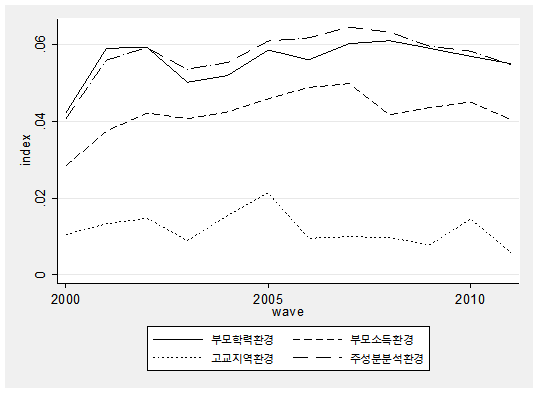
\includegraphics[width=\textwidth]{figure/goms_goi_byenv.png}
    \label{fig:goms_goi_byenv}
\end{figure}

환경-입시유형별 GOI 지수를 살펴본다.
PCA, 학력, 소득의 세 환경에서 일반수시 입학자들 간의 기회불평등이 일반정시 입학자들 간의 기회불평등보다 항상 높았다.
 이는 수시가 정시보다 기회불평등한 대입전형이라는 대중의 인식을 구체적으로 입증한 것이다.
 두 전형간 지수의 격차는 일반정시의 기회불평등이 높아지는 형태도 줄어들고 있어, 정시가 수시에 비해 상대적으로 기회평등했다고 해도 정시제도 자체가 기회평등하지는 않다는 점을 명심해야 한다.
 지역환경에서 기회불평등은 앞서의 환경과 다른 모습이다.
 일반수시에 의한 기회불평등은 2003년부터 꾸준히 감소해 2005년부터는 일반정시보다 현저히 낮다.
 이는 도시 이외지역의 고교가 내신획득에 유리하다는 점과 지역균형선발과 같은 직접적인 지역기회불평등 해소제도의 역할이 작용한 결과로 해석된다.

\begin{figure}
    \centering
    \caption{가구환경간 대학입학성과의 지니기회불평등도 추세: 입시유형별 비교}
    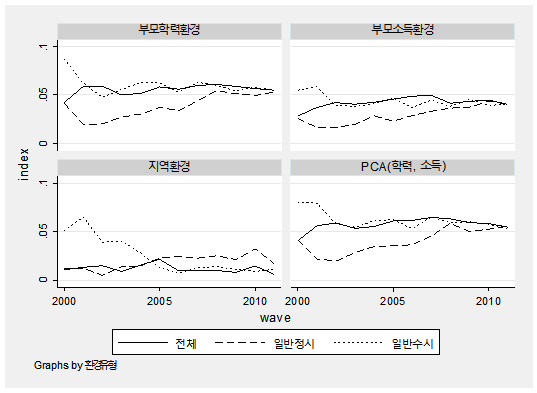
\includegraphics[width=\textwidth]{figure/goms_goi_byent.png}
    \label{fig:goms_goi_byent}
\end{figure}

\subsection{교육성취의 개천용기회불평등지수 분석 결과}
지금부터는 개천용기회불평등지수(RRI)를 살펴본다.
먼저 5점 척도에 의한 환경별 개천용지수의 추이부터 살펴본다.
 RRI에서 지수의 크기는 GOI와 마찬가지로 PCA, 학력, 소득, 지역 순으로 나타났다.
 연도마다 지수의 변동 폭이 커 보이는 데 이는 성공의 기준점이 상위 약 2.8\%로 극히 적은 수를 대상으로 하기 때문이다.
  PCA와 학력을 기준으로 했을 때 평균 약 0.7의 수치를 보이는데, 최우수 대학 및 학과에 진학함에 있어 심각한 기회불평등이 존재함을 알 수 있다.
  부모소득을 환경으로 하면 평균 약 0.6으로 여전히 큰 기회불평등이 존재하지만, PCA나 학력에 비해 상대적으로 낮은 것으로 나타났다.
  출신고교지역을 환경으로 할 경우는 지수는 평균 약 0.3으로 다른 환경들에 비해 현저히 낮고 그 정도도 크게 심각하지 않다.
 
\begin{figure}
    \centering
    \caption{가구환경간 대학입학성과의 개천용기회불평등도 추세}
    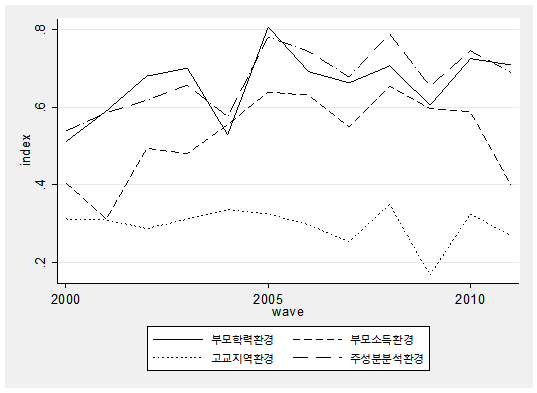
\includegraphics[width=\textwidth]{figure/goms_rri_byenv.png}
    \label{fig:goms_rri_byenv}
\end{figure}

남성 간-여성 간 RRI 차이는 앞서 GOI의 경우와 마찬가지로 차이가 비해 적다.
GOI와는 다르게 부모 학력, 부모소득, 고교지역, PCA의 모든 환경에서는 여성의 기회불평등이 남성보다 다소 높다.
특히 지역 환경에서 경우 다른 환경에 비해 남성 간과 여성 간의 불평등지수의 격차가 가장 크게 나타났다.
여성의 경우 도 지역에서 명문대 및 의대가 있는 도시와 같은 다른 지역으로 유학을 가야 하는 점에 대한 부담감이 작용할 가능성이 있다.


\begin{figure}
    \centering
    \caption{가구환경간 대학입학성과의 개천용기회불평등도 추세: 성별 비교}
    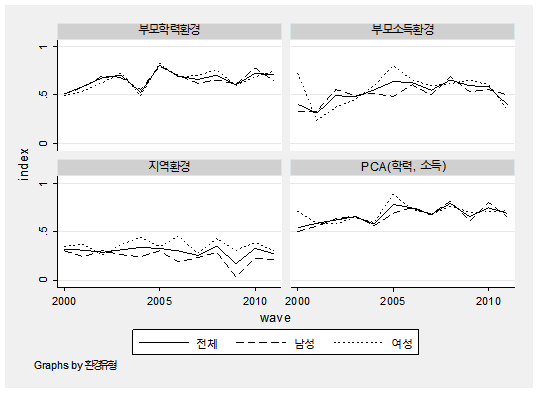
\includegraphics[width=\textwidth]{figure/goms_rri_bysex.png}
    \label{fig:goms_rri_bysex}
\end{figure}

환경-입시유형별 RRI는 GOI 경우와 동일하게 정시보다 수시가 기회불평등 한 것으로 보인다.
특히 지역 환경에서 정시, 수 시간의 격차가 다른 환경보다 매우 크게 나타난다.
 앞서 살펴본 지니기회불평등지수와 환경, 환경-성별 개천용기회불평등지수의 모든 경우에서 지역 환경은 기회불평등 정도가 다른 환경에 비해 현저히 낮고 그 세부구분에서도 차이가 없었다.
 반면 학생이 수시입학을 통해 최상위 교육성취를 얻는데 거주지역이 그 자체로 상당한 기회불평등을 일으키는 것으로 나타났다.
 해당 최상위 대학들의 수시 비중이 높다는 점을 고려했을 때, 이들의 지역균형전형이 충분하지 않음을 짐작할 수 있다.
 2000년과 2001년은 지수 값이 1인 경우가 나오는데 2002년 이후부터 수시정원이 확대되기 시작한 사실과 정시 대 수시 비율이 10:1인 점을 감안하여 예외적인 경우로 보는 것이 타당하다.

\begin{figure}
    \centering
    \caption{가구환경간 대학입학성과의 개천용기회불평등도 추세: 입시유형별 비교}
    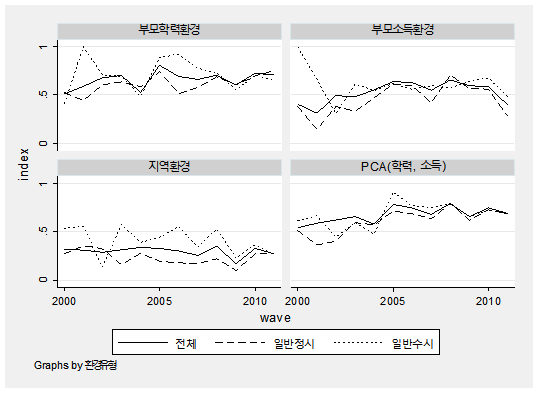
\includegraphics[width=\textwidth]{figure/goms_rri_byent.png}
    \label{fig:goms_rri_byent}
\end{figure}


\section{대학졸업 후 경제적 성취의 기회불평등}
지금부터는 조사대상의 소득의 기회불평등을 분석한다.
모든 취업자를 대상으로 분석하는 경우는 졸업 직후의 경제적 기회불평등을 분석하는데 의의가 있는 반면, 정규근로자 및 자영업자로 제한하여 분석을 하는 것은 조사대상의 향후 소득의 기회불평등 전망에 더 유의미한 자료가 된다.
누적분포 및 확률지배관계 결과는 모든 직업만을 대상으로 진행하였으며, 지수도출은 두 경우를 각각 제시한다.

\subsection{누적분포함수}
앞서와 마찬가지로 주성분분석과 출신고교지역 두 가지 환경에 대한 누적분포를 제시한다.
주성분분석환경에서는 유리한 환경일수록 소득분포가 오른쪽 또는 아래쪽에 위치하여 소득획득에 평균적으로 유리할 것을 알 수 있다.
출신고교지역의 경우는 환경유형별 분포가 거의 유사하여 출신 지역에 의한 소득의 기회불평등이 미미할 것이라고 짐작할 수 있다.
두 환경 모두에서 환경유형간 분포의 차이가 줄어드는 것으로 보여 전반적인 기회불평등도가 감소추세임을 유추할 수 있다.

\begin{figure}
    \centering
    \caption{코호트별 주성분분석환경하 소득의 누적분포}
    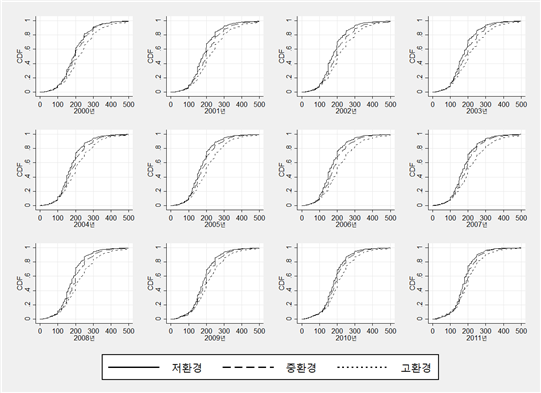
\includegraphics[width=\textwidth]{figure/gomse_cdf_bypca.png}
    \label{fig:gomse_cdf_bypca}
\end{figure}

\begin{figure}
    \centering
    \caption{코호트별 출신고교지역환경하 소득의 누적분포}
    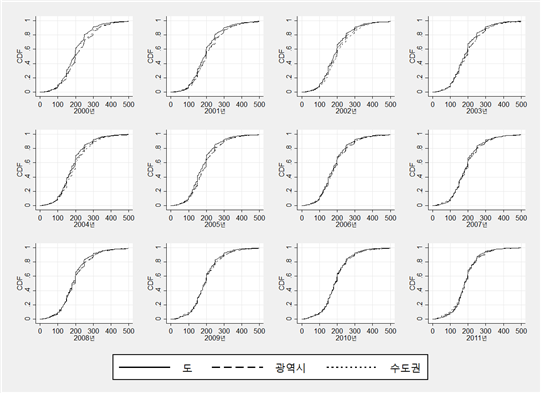
\includegraphics[width=\textwidth]{figure/gomse_cdf_byrgn.png}
    \label{fig:gomse_cdf_byrgn}
\end{figure}

\subsection{확률지배결과}
소득의 경우 분포의 양극단, 다시 말해 매우 낮은 소득이나 매우 높은 소득의 범주에서 환경 간에 분포가 교차하는 경우가 자주 발생한다.
그 결과 자료의 전반에서 확률지배관계가 존재하더라도 없는 것처럼 보이게 한다.
따라서 검증구간에 일부 제한을 두는 것이 필요한데, 본 분석에서는 대부분 자료를 포함할 수 있는 월평균소득 100만 원에서 400만 원 사이의 경우에 대하여 확률지배검증을 시행했다.

\begin{table}[htbp]
    \centering
    \caption{PCA환경하 소득 누적분포의 확률지배 검증결과}
    \begin{tabular}{c|c|c|c|c|c|c}
\hline & \multicolumn{3}{|c|}{중환경} & \multicolumn{3}{c}{고환경} \\
\hline \multirow{4}{*}{저환경} & $=$ & $<_{1}^{**}$ & $<_{1}^{***}$ & $<_{1}^{***}$ & $<_{1}^{***}$ & $<_{1}^{***}$ \\
\cline{2-7} & $<_{2}^{*}$ & $?$ & $<_{1}^{*}$ & $<_{1}^{***}$ & $<_{1}^{***}$ & $<_{1}^{***}$ \\
\cline{2-7} & $<_{2}^{*}$ & $=$ & $<_{2}^{**}$ & $<_{1 }^{***}$ & $<_{1 }^{***}$ & $<_{1 }^{***}$ \\
\cline{2-7} & $=$ & $?$ & $?$ & $<_{1}^{***}$ & $<_{1}^{***}$ & $<_{1}^{***}$ \\
\hline \multirow{4}{*}{중환경} & 2000 & 2001 & 2002 & $<_{1}^{***}$ & $<_{1}^{*}$ & $<_{1}^{***}$ \\
\cline{2-7} & 2003 & 2004 & 2005 & $<_{1}^{***}$ & $<_{1}^{**}$ & $<_{1}^{***}$ \\
\cline{2-7} & 2006 & 2007 & 2008 & $<_{1}^{***}$ & $<_{1}^{***}$ & $<_{1}^{**}$ \\
\cline{2-7} & 2009 & 2010 & 2011 & $<_{1}^{***}$ & $<_{1}^{***}$ & $?$ \\
\hline
\end{tabular}
    \\
    \confer{집단별 상하위 5\%를 각각 제외하고 검증. $=$ 은 동일한 확률분포, $<_{1}$은 행이 열에 1차 확률지배, $<_{2}$는 행이 열에 2차 확률지배 당하는 관계,  $?$는 확률지배관계를 확인 불가능한 경우임. ($*: \alpha = 0.5, **: \alpha = 0.01, ***: \alpha = 0.001$.)}
    \label{tab:gomse_dom_bypca}
\end{table}

주성분분석 환경하에 확률지배검증 결과 거의 모든 연도에서 모든 환경 쌍에 기회불평등이 존재하는 상황을 확인했다.
고환경은 저, 중환경에 대하여 뚜렷하게 확률지배를 하는 것을 확인했다.
반면, 저환경과 중환경 사이에는 동일분포로 판단되는 경우도 있었다.
소득의 기회불평등은 고환경만 절대적으로 유리한 형태로 존재함을 확인했다.
지역의 경우 누적분포함수에서 유추할 수 있듯이 거의 모든 환경 유형의 쌍에서 확률지배검증이 안 되거나 동일분포로 판단되어 출신고교지역에 의한 소득의 기회불평등은 거의 없는 것을 확인했다.

\begin{table}[htbp]
    \centering
    \caption{PCA환경하 소득 누적분포의 확률지배 검증결과}
    \begin{tabular}{c|c|c|c|c|c|c}
\hline & \multicolumn{3}{|c|}{중환경} & \multicolumn{3}{c}{고환경} \\
\hline \multirow{4}{*}{저환경} & $?$ & $?$ & $=$ & $?$ & $?$ & $<_{1}^{***}$ \\
\cline{2-7} & $?$ & $<_{2}^{**}$ & $?$ & $?$ & $<_{1}^{*}$ & $?$ \\
\cline{2-7} & $=$ & $?$ & $?$ & $=$ & $?$ & $?$ \\
\cline{2-7} & $=$ & $=$ & $?$ & $?$ & $=$ & $?$ \\
\hline \multirow{4}{*}{중환경} & 2000 & 2001 & 2002 & $=$ & $=$ & $<_{2}^{***}$ \\
\cline{2-7} & 2003 & 2004 & 2005 & $=$ & $?$ & $?$ \\
\cline{2-7} & 2006 & 2007 & 2008 & $=$ & $=$ & $=$ \\
\cline{2-7} & 2009 & 2010 & 2011 & $=$ & $=$ & $=$\\
\hline
\end{tabular}
    \\
    \confer{집단별 상하위 5\%를 각각 제외하고 검증. $=$ 은 동일한 확률분포, $<_{1}$은 행이 열에 1차 확률지배, $<_{2}$는 행이 열에 2차 확률지배 당하는 관계,  $?$는 확률지배관계를 확인 불가능한 경우임. ($*: \alpha = 0.5, **: \alpha = 0.01, ***: \alpha = 0.001$.)}
    \label{tab:gomse_dom_byrgn}
\end{table}

\subsection{소득의 지니기회불평등지수 분석 결과}
환경별 GOI의 추이는 PCA와 부모소득이 거의 동일하고, 부모학력, 지역 순으로 높게 측정된다.
모든 환경에 대하여 GOI의 값이 거의 절반 수준에 머물러, 교육의 성취보다 소득에서 환경의 영향이 훨씬 낮음을 알 수 있다.
앞서 교육성취와는 다르게 주성분분석과 소득환경의 경우가 지수 값의 크기와 성향이 매우 유사하여, 소득성취의 기회불평등은 부모의 소득에서 주로 기인함을 알 수 있다.
모든 환경변수 교육성취에서는 2008년부터 지수의 전반적인 하락세가 있었는데 소득에서는 한 해 빠른 2007년부터 하락세가 보인다.
지역에 의한 기회불평등은 역시 거의 없는 수준이다.
모든직업을 대상으로 할 경우보다 정규직$\cdot$자영업을 대상으로 할 경우의 불평등도가 높게 나오는데, 이는 정규직이라는 우월한 직위를 획득하는데 대한 기회불평등 역시 존재함을 반영한다.

\begin{figure}
    \centering
    \caption{환경별 소득의 지니기회불평등지수 추이}
    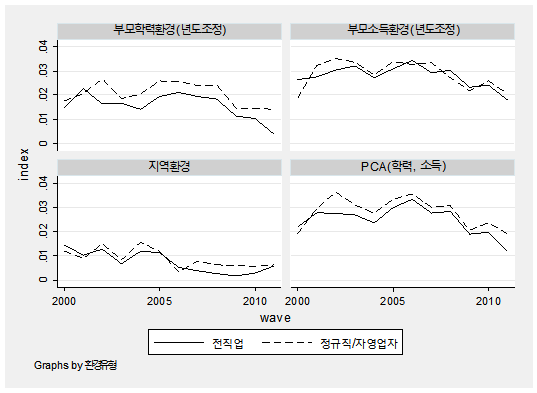
\includegraphics[width=\textwidth]{figure/gomse_goi_byenv.png}
    \label{fig:gomse_goi_byenv}
\end{figure}

환경-입시유형별 GOI 지수는 <그림 \ref{fig:goms_goi_byent}>에 나타나 있다.
정규직$\cdot$자영업자의 경우 48개 조사시점 가운데 총 38개 조사시점에서 일반수시 졸업자간의 기회불평등이 일반정시 졸업자간의 기회불평등보다 유의미하게 높았다.
이는 매우 흥미로운 결과인데 입시제도가 대학입학에 일시적인 영향을 주는 것을 넘어서 졸업 이후의 소득획득에도 관계가 있다고 해석할 수 있다.
하지만 대입유형은 수험생들이 선택할 수 있고 정시와 수시의 정원은 수험생들과 무관하게 바뀌고 있는 등의 요소에 대한 통제가 없는 본 연구에서 특정 대입제도가 미래 개인들의 소득획득에 인과관계가 존재한다고 이야기 할 수 없다.

\begin{figure}
    \centering
    \caption{환경-대입유형별별 소득획득의 개천용불평등지수 추이}
    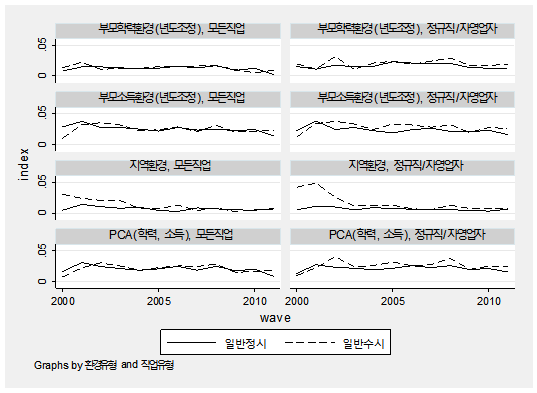
\includegraphics[width=\textwidth]{figure/gomse_goi_byent.png}
    \label{fig:gomse_goi_byent}
\end{figure}

\subsection{소득의 개천용기회불평등지수 분석 결과}
지금부터는 개천용기회불평등지수(RRI)를 통해 고소득 획득에서 기회불평등 양상을 살펴본다.
 앞서 대학입학의 경우 최상위인 5점을 성공의 척도로 삼았는데, 이들은 상위 약 2.8\% 이었다.
 대학입학과 결과 비교를 위해 소득에서도 상위 2.8\%를 성공의 기준으로 한다.
 하지만 소득 2.8\%는 성공의 기준으로 지나치게 엄격하다.
 또한 불리한 환경에서 성공하는 개인의 수가 현저히 줄어들어 개천용불평등지수 표준오차가 과대 측정되고, 남녀간 또는 대입유형간 지수비교에서 유의성이 현저히 감소할 수 있다.
 그래서 또다른 성공의 기준으로 소득 상위 10\%를 이용한 지수값을 같이 제시한다.
 
\begin{figure}
    \centering
    \caption{환경별 소득의 개천용기회불평등지수 추이: 상위 2.8\% 성공기준}
    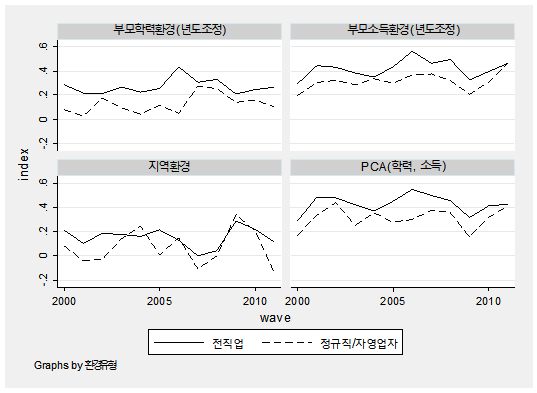
\includegraphics[width=\textwidth]{figure/gomse_rri_byenv_28.png}
    \label{fig:gomse_rri_byenv_28}
    \confer{성공기준은 코호트별 소득 상위 2.8\%.}
\end{figure}

 <그림 \ref{fig:gomse_rri_byenv_28}>는 상위 2.8\%소득을 성공의 기준으로 한 RRI의 추이다.
 GOI의 경우 대학입학을 성취로 했을 경우에 비하여 소득을 성취로 한 지수값이 거의 절반 가깝게 하락했던 반면 RRI에서는 지수값은 하락하지만 하락폭은 GOI에 비해 크지않은 것을 알 수 있다.
 환경별로는 GOI와 마찬가지로 PCA 및 소득, 학력, 지역 순으로 나타났다.
 PCA 소득을 환경으로 했을 때 약 지수 값이 0.4 근처에 있어, 불리한 환경에 속한 개인들은 10명 중 4명은 환경의 영향으로 상위 2. 8\% 소득의 획득에 실패한다고 할 수 있다.
 하지만 0.6-0.7 사이에 위치하는 대학입학의 지수 값과 비교한다면 불평등의 정도가 현저히 낮음을 알 수 있다.
 지역의 경우 음의 지수값이 나오는 코호트가 있는데 이는 도지역 출신자가 전체 인구에서의 비율보다 소득상위 2.8\%에서 더 많이 존재한다는 의미로 지역환경은 정규직/자영업자의 고소득 획득에 불리한 영향을 거의 주지 않음을 알 수 있다.

\begin{figure}
    \centering
    \caption{환경별 소득의 개천용기회불평등지수 추이: 상위 10\% 성공기준}
    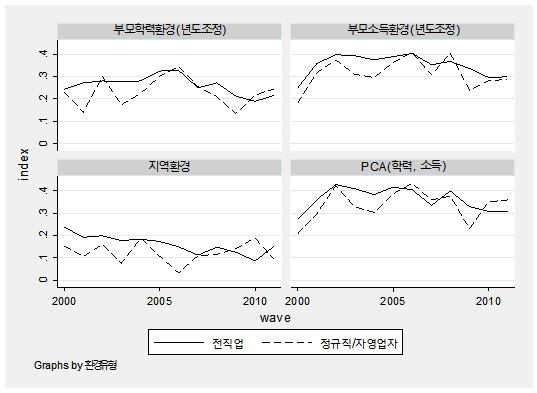
\includegraphics[width=\textwidth]{figure/gomse_rri_byenv_10.png}
    \label{fig:gomse_rri_byenv_10}
\end{figure}

상위 10\% 소득을 성공기준으로 하는 <그림 \ref{fig:gomse_rri_byenv_10}>는 완화된 성공의 기준으로 인해 <그림 \ref{fig:gomse_rri_byenv_28}>보다 수치가 전반적으로 낮다.
 전직업의 경우 코호트별 지수의 변동폭이 줄어드는 반면 정규직$\cdot$자영업자는 변동폭이 늘어나는 상반된 모습을 보였다.
 GOI의 경우 2009-2011년 코호트에서 하락하는 추세였으나 RRI에서는 두 성공기준 모두에서 상승하는 양상을 나타냈다.
 이는 성공기준에 속하는 인원 가운데 열악한 환경에 속한 개인들의 수는 줄어든 반면 중간 환경에 속한 개인들의 수가 크게 늘었기 때문이다.

\begin{figure}
    \centering
    \caption{환경별 소득의 개천용기회불평등지수 추이: 상위 10\% 성공기준}
    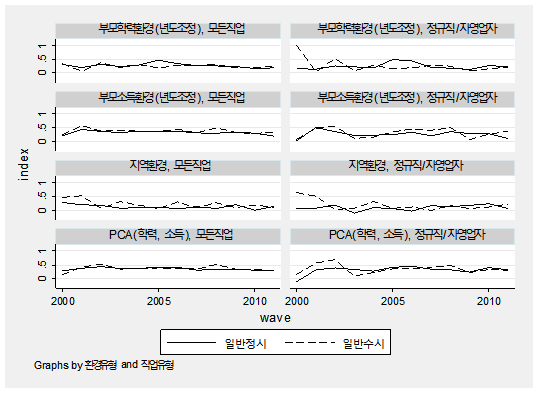
\includegraphics[width=\textwidth]{figure/gomse_rri_byent_10.png}
    \label{fig:gomse_rri_byent_10}
\end{figure}

환경-입시유형별 RRI는 GOI 경우와 특정한 입시유형이 성공에서 더 기회불평등한 경우는 없다.
 <그림 \ref{fig:gomse_rri_byent_10}>을 보면 일반정시와 일반수시의 추이가 대부분의 경우에서 수시로 교차하는 것을 확인할 수 있다.
 2000년과 2001년은 대학입학의 경우와 마찬가지로 수시로 합격한 개인이 적은 탓에 유의미한 결과가 아닌 것으로 해석해야 한다.

\section{소결론 및 시사점}

가구의 사회경제적 지위에 따라 대학진학 성과 및 생애 첫 소득의의 기회불평등이 조사 기간 전체에 걸쳐 뚜렷하게 존재하는 것으로 나타났다.
지역에 따른 성취의 기회불평등은 대학진학 및 소득 모두에서 불분명하지만, 광역시와 시군구 간의 기회불평등은 대학진학에서 뚜렷하게 나타났다.

대학진학에서 지니기회불평등지수는 2007년을 전후로 완만한 상승에서 완만한 하강으로 바뀐다.
 개천용기회불평등지수는 2007년 이후에도 상승세를 보였고, 특히 수준이 매우 높아 조사 기간 말에는 열악한 환경에서 기회불평등으로 최상위권 대학진학에 실패할 확률이 70\%에 이르는 것으로 나타났다.
 입시 전형별로 일반수시 합격자간 기회불평등이 일반정시 합격자간 기회불평등보다 높은 것으로 나타났다.
 그러나 일반정시 합격자간 기회불평등도는 조사 기간에 걸쳐 꾸준히 상승하여 수시와 정시 간의 기회불평등도 격차는 크게 줄어들었다.
 이러한 현상이 정시 비중이 2002년 70\%에서 2019년 현재 40\%대로 감소하는 상황과 관련된 것인지에 대하여 추가적인 연구가 필요하다.

소득의 경우 대학진학에 비해 기회불평등의 정도가 현저히 낮은 것으로 나타났다.
 소득의 지니기회불평등지수는 2008년 이후부터 완만한 내림세를 보인다.
 개천용기회불평등지수 역시 2007년부터 하락하지만 2009년부터는 다시 상승하는 반대 추세를 보였다.
 대학진학보다는 낮은 수치이지만, 열악한 환경에서 기회불평등으로 고소득 획득에 실패할 확률이 40\%라는 결론은 무시할 수 없는 수치이다.
 입시 전형별로 일반수시로 대학에 들어간 개인들 사이의 기회불평등이 일반정시로 대학에 들어간 개인들 간의 기회불평등보다 유의하게 높았다.
 지니기회불평등 지수로 확인한 입시유형간의 소득획득의 기회불평등은 개천용기회불평등지수로 분석한 고소득 획득에서는 유의미한 차이가 없었다.
 성별의 경우 소득획득에서 명백한 기회불평등이 존재함을 확인했다.

본 연구는 대졸자를 대상으로 하였기 때문에 교육 및 경제적 성취의 기회불평등을 과소 측정하는 문제를 안고 있다.
 특히 1절에서 본것과 같이 열악한 환경일수록 수능에 응시하지 않고 따라서 대학진학 이루어지지 않았기 때문에 열악한 환경에 처한 집단의 성취가 과대측정되는 문제가 있다.

향후 연구과제는 다음과 같다.
본 연구는 성별, 입학유형별로 제한을 통해 정시입학자간, 수시입학자간 기회불평등에 대한 분석은 수행하였다.
 이를 통해 성별과 대입유형이 성취의 기회불평등에 영향을 준다는 점은 확인했다.
 하지만 이러한 요소가 성취와 성취의 기회불평등과 어떤 관련이 있는가에 대한 구체적인 결론은 향후 연구되어야 할 과제다.
 특히 성별에 의해 유발되는 기회불평등의 정도와 대입유형과 소득과의 관계가 그러하다.

\chapter{한국의 소득획득의 기회불평등}
\section{서론}

개인의 성취는 노력, 환경, 그리고 운이 복합적으로 작용하여 결정된다.\footnote{본 연구는 \citet{onj17}의 연구에 노동패널의 최신 자료를 판올림한 글이다.} 존 롤즈(\citeauthor{Rawls99})는 동일한 천부적 능력과 야망을 가진 사람들이 그 사람의 가정환경, 상속된 부의 크기, 인종, 성 등과 무관하게 동등한 성취의 전망(prospects of success)을 가질 때 ``공정한 기회평등''이 보장된다고 하였다.\footcite[p. 63.]{Rawls99} 이러한 롤즈의 입장은 드워킨(\citeauthor{dworkin81a}), 아네슨(\citeauthor{arneson91}), 코헨(\citeauthor{cohen89}), 로머(\citeauthor{Roemer98}) 등에 의하여 평등주의의 대표적인 분배 원칙으로 자리 잡게 되었다.\footnote{\citet{dworkin81a, dworkin81b}, \citet{arneson91}, \citet{cohen89}, \citet{Roemer98}}

노력에 따라 발생하는 불평등에 대해서는 마땅히 그 개인이 책임져야 하겠지만 개인의 의지와 무관하게 주어지는 환경에 따라 발생하는 불평등에 대해서까지 개인에게 책임을 지워서는 안 된다는 것이 본 논문의 전체에 일관된 기회평등에 대한 기본 입장이다. \footcite[p.5.]{Roemer98} 즉, 개인에게 도덕적 책임이 없는 환경이 성취에 미치는 영향은 모든 사람들에게 중립적으로 작용하여야 하고, 따라서 더 이로운 환경도 더 불리한 환경도 없도록 해야 한다는 것이다. 이러한 기회평등의 기본 정신에 대해서는 상당히 높은 수준의 사회적 합의가 있으며 복지선진국들이 추구하는 사회정책의 기본 방향이기도 하다.

기회불평등한 사회에서는 개인의 의지나 선택과 관계없이 타고난 사회$\cdot$경제적 환경이 그 사람의 성취 전망의 우열을 결정하게 된다. \citet{letl08, letl09}은 환경 별로 얻어진 성취(소득) 분포들 간의 ``확률지배관계''가 존재할 경우 기회불평등이 존재한다고 정의하고 미국과 유럽의 주요 국 소득자료를 통하여 소득기회불평등의 존재와 크기를 분석하였다. 본 연구의 주된 목적은 이러한 \citeauthor{letl08}의 실증적 방법론을 활용하여 우리나라의 소득 기회불평등의 존재와 크기를 분석하고 선행연구와 비교하는 것이다.

급속한 경제성장에도 불구하고, 우리나라의 소득불평등은 1990년대 초반기 낮은 수준을 유지해 왔었고 세대 간 계층 상승의 기회도 비교적 높은 수준이었던 것으로 알려져 있다. 이러한 고성장-저불평등의 구조는 1990년대 중반이후 흐려지기 시작하여, 2000년을 지나 현재에 이르기까지 소득불평등은 빠른 속도로 악화되었다. 높은 불평등과 양극화를 겪으면서 기회평등에 대한 국민들의 신뢰는 크게 약화되었고 자녀 교육을 통한 신분상승의 희망도 사라지고 있다.

이러한 주관적 인식의 급격한 변화와 달리 세대 간 계층이동에 대한 여러 선행연구들은 비교적 낙관적인 결론을 보였다. 본 연구와 동일한 한국노동패널 자료를 이용한 \citet{cnh11}과 \citet{yang12}은 세대 간 소득탄력성(부모소득상승률에 대한 자녀소득 상승률의 비율)을 0.37이하로 추정하여 OECD국가 평균 이하었다. 이는 우리나라의 세대 간 계층이동성이 OECD 평균 보다 높은 것을 의미한다. \footnote{선행연구인 \citet{kim09}과 \citet{ketl09} 등에서는 이보다 더 낮은 탄력성이 보고되기도 하였다.} 따라서 적어도 세대 간 소득탄력성의 기준으로 볼 때 우리나라의 기회불평등은 비교적 낮은 수준이라는 것이다.

이렇게 한국노동패널 자료 분석에서 나타난 결과가 앞서 인용된 통계청 「사회조사」의 결과와 차이가 나는 이유로는, 우선 자료에 반영된 성인들의 대부분이 1990년대 중반 이전에 초중고 교육을 받은 세대에 속하는 점을 들 수 있다. 이 세대에서 교육을 통한 계층상승의 기회가 비교적 공평하게 주어졌다는 주지의 사실에 비추어 볼 때 높은 세대 간 계층이동성은 자연스러운 결과라 할 수 있다. 둘째로, 설문조사에 나타난 세대 간 계층이동에 대한 주관적 인식이 세대 간 소득탄력성 만으로 나타내기 어려운 기회불평등의 양상들을 반영한 결과일 수 있다는 점이다. 가령, 눈에 띄게 변화한 대학진학에 있어서 소득계층 및 지역 간 격차와 계층 사다리로서의 교육의 역할이 약해진 점 등을 들 수 있다.

\citet{knl08}은 기회불평등을 최소화하는 세율과 실제 세율을 비교하는 방식(\citet{retl03})을 적용하여 우리나라의 기회불평등도가 OECD국가들 중에서 미국과 이탈리아처럼 높은 나라에 속함을 보인 바 있다.
이처럼 세대 간 소득 탄력성만으로는 포착하기 어려운 기회불평등의 다차원적 연구를 통하여 소득 계층이동에 대한 주관적 인식 변화에 대한 합당한 설명을 제시할 수 있는 가능성은 열려 있다고 볼 수 있다.  
본 연구와 동일한 방법을 활용하여 교육적 성취(대학입학 수학능력평가 성적)의 기회불평등을 연구한 \citet{ohetl16}에서는 우리사회에 교육성취의 기회불평등이 뚜렷하게 나타남을 보여주고 있다.
더 이상 우리사회에서 교육의 계층사다리 기능이 작동하기 어렵다는 이러한 결과는 앞서 소개된 통계청 조사를 잘 설명한다고 볼 수 있다.
교육 자료는 어린 청소년들을 대상으로 하여 성인을 대상으로 하는 소득 자료 보다 세대 간 계층이동성에 대한 주관적 인식 변화의 흐름을 더 잘 반영한다고 볼 수 있다.
 본 연 구에서는 선행연구들에서 사용한 한국노동패널의 가구소득자료를 기초로 \citet{letl08, letl09}에 소개된 기회불평등의 존재와 크기에 대하여 살펴 볼 것이다.
 
 만일 A라는 환경에 놓인 사람이 B라는 환경에 놓인 사람보다, 동일한 노력을 할 때 항상 더 높은 성취의 가능성을 갖는다면 두 사람에게 보장된 성취의 기회가 평등하다고 볼 수 없고 A에게 더 우월한 성취의 기회가 보장된다고 말할 수 있다.
 어떤 두 환경 사이에도 이처럼 하나가 다른 하나보다 더 우월한 성취의 기회를 보장한다고 할 수 없을 때 기회평등이 달성되는 것이다.
 이러한 기회평등 개념에 기초하여 \citet{letl08, letl09}은 미국, 이탈리아, 노르웨이, 스웨덴 등의 주요 선진국에서 부모 학력별 (혹은 직업별) 소득분포들을 도출하고 이들 간에 우열관계의 유무를 검증하는 방식으로 기회평등의 유무를 확인하였다.

본 연구에서는 \citeauthor{letl08}과 동일하게 가구주의 학력과 직업이라는 두 가지 환경변수를 활용하여 상이한 환경 간의 기회불평등의 존재 여부를 살펴보았다.
 분석 결과 두 환경 변수 모두에 있어서 소득 성취의 기회불평등이 존재하는 것으로 나타났다.
 \citet{letl08, letl09}에서 얻어진 결과와 비교할 때, 우리나라의 기회불평등은 비교적 기회불평등이 뚜렷한 미국, 프랑스, 이태리와 유사하게 나타나고 기회불평등이 존재하지 않거나 그 정도가 낮은 스웨덴, 노르웨이, 독일과는 다르게 나타났다.
 또한 개천용기회불평등지수(최상위소득계층에서의 최하위환경비율)를 이용한 분석에서 2000년대 초반 이후로 기회불평등도가 다소 상승하는 경향이 있다는 사실을 확인할 수 있었다(개천용지수는 본 연구와 동시에 진행된 교육기회불평등에 대한 연구, \citet{ohetl16}에서도 소개된 바 있다).
 
기회평등의 원칙은 \citet{Roemer98}와 \citet{letl08, letl09}에 의하여 실증 모형에 도입되었고 경험적 분석에 활용될 수 있게 되었다.
 \citet{letl08}은 프랑스 소득자료를 바탕으로 부모의 직업을 환경변수로 하여 총 여섯 개의 서로 다른 집단간에 기회불평등이 존재하는지 여부를 검증하여 기회의 불평등이 존재함을 보였다.
 \citet{letl09}는 동일한 연구방법을 유럽각지의 8개국과 미국을 대상으로 실시하여 스웨덴, 노르웨이 같은 북유럽 국가의 경우 기회평등한 사회임을 보였다.
 
기회불평등에 대한 국내 선행연구로 \citet{knl08}와 \citet{knl11}은 아버지의 학력과 직업이 자식의 소득획득 기회에 중요한 영향을 미친다는 사실을 밝힌 바 있다.
 또한 아버지의 학력, 성별, 출생년도, 성장기 지역, 형제자매 수 등의 여러 환경요인들을 고려한 \citet{jnl16}의 최근 연구에서도 소득불평등에서 환경이 차지하는 비중이 매우 높다는 것이 확인되었다.

\section{모형과 기본개념}
개인의 소득은 개인의 노력뿐만 아니라 개인의 선택과 무관하게 주어지는 사회경제적 환경(부모의 경제력과 학력), 선천적인 재능, 그리고 여러 우연적 요인들에 의하여 결정된다.
노력의 차이가 발생시킨 소득 격차는 일정 부분 용인되어야 하겠지만 사회경제적 환경의 차이가 야기하는 불평등까지 용인할 수 없다는 것이 본 연구의 기본적인 전제이다.

환경 $c$와 노력 $e$가 다른 우연적인 요인들과 결합되어 만들어내는 소득 $y$의 조건부 확률분포를 $y=F(y|c)$라 하자. 
\footnote{본 연구의 기본모형은 소득 기회 불평등에 대한 연구인 \citet{letl08, letl09}의 모형을 따르고 있다.}
즉 임의의 두 환경 에 대해 가 성립한다는 의미이다.
가장 강한 형태의 기회평등의 원칙은, 임의의 두 환경 $c,c' \in C$에 대하여 각 노력수준 에서 결정되는 수능성적의 분포가 동일해야 한다는 조건 $F(\cdot | c) = F(\cdot | c')$으로 정의할 수 있다. 
하지만 이러한 기회평등은 과도하게 이상적이라 할 수 있고, 본 연구에서는 이를 완화한 \citet{letl08, letl09}의 기회평등 개념을 활용한다. 
\citeauthor{letl08}의 두 논문이 실증모형, 기본개념 그리고 이론적 정리들을 자세히 소개하고 있으나 완결성을 위하여 핵심적인 내용들을 본 절에서 간략히 다시 정리할 것이다.

\subsection{기회불평등}
 
 상이한 두 환경 $c$와 $c'$에서 개인의 노력 $e$는 각각 $F(\cdot |c,e)$와 $F(\cdot |c',e)$의 소득 전망을 제공한다고 볼 수 있다. 
만약 모든 노력수준 $e$와 모든 소득수준 $y$에서
\begin{equation}
    F(x | c) \leq F(x | c')
    \label{eq:klips_fdom}
\end{equation}
이 성립하면 환경 $c'$에서서 노력 수준에 무관하게 항상 일정소득 $y$를 초과하는 소득을 획득하는데 실패할 확률이 환경 $c$에서 보다 크거나 같다는 것을 의미한다.
이는 소득획득의 전망의 관점에서 환경 $c'$이 환경 $c$보다 열악하다는 것이다.
이처럼 적어도 두 개의 환경 $c,c'$에서 식 (\ref{eq:klips_fdom})이 성립하고 적어도 하나의 소득수준에서 이 부등식이 강부등식으로 성립하여 두 환경사이에 제 1차 확률지배관계가 형성되는 경우에 제1차 기회불평등이 존재한다고 정의한다.

식 (\ref{eq:klips_fdom})의 제1차 확률지배관계를 제2차 확률지배관계로 대체하여, 모든 노력수준 $e$와 모든 소득수준 $x$ 에서,
\begin{equation}
   \int_{0}^{x} F(y | c)\,dy \leq \int_{0}^{x} F(y | c')\,dy
    \label{eq:klips_sdom}
\end{equation}
의 관계가 성립하고 적어도 하나의 $x$에서 강부등호 관계가 성립하는 두 개의 환경 $c,c' \in C$이 존재할 때 제2차 기회불평등이 존재한다고 정의한다. 

제1차(제2차) 기회평등은 이와 같이 제1차(제2차) 기회불평등이 존재하지 않을 때 성립한다.
\footnote{\citet{letl09}에서 EOP-W1, EOP-W2 참고.} 
 기회평등이 성립하더라도 상이한 두 환경에서 얻어지는 성취의 확률분포들이 동일할 필요가 없을 뿐만 아니라 두 환경 중 하나에서 성취의 기댓값의 더 큰 것도 허용된다.
 또한 모든 노력 수준에서 확률지배관계가 성립해야 기회불평등이 존재하는 것으로 정의하고 있어서 적어도 한 노력 수준에서만 확률지배관계가 없다면 기회평등이 성립하게 된다. 
 이처럼 본 연구에서 정의하는 기회평등은 최소한의 원칙이라는 점에 주목할 필요가 있다.
 
두 환경 사이에 식 (\ref{eq:klips_fdom})과 같은 기회불평등이 존재하면, 어떤 효용함수를 상정하더라도 환경 $c$의 소득분포 $F(\cdot |c,e)$에서 기대효용이 환경 $c'$의 소득분포 $F(\cdot |c,e)$에서 보다 더 클 것이다.
  즉, 항상 환경 $c$가 $c'$ 보다 선호될 것이다.
  소득에 대하여 위험기피적인 선호를 가정하면, 두 환경 사이에 식 (\ref{eq:klips_sdom})와 같은 기회불평등이 존재할 때도 항상 환경 $c$가 $c'$ 보다 더 큰 기대효용 가져 선호될 것이다.
  
만일 노력 수준 그 자체가 환경에 영향을 받는다면 앞에서 정의한 기회불평등 개념은 기회불평등의 기본원리를 적절히 담고 있다고 볼 수 없을 것이다.
 가령 환경 $c$가 환경 $c'$ 보다 노력하기 용이한 환경이라고 하자.
 각 노력에서 소득의 확률분포가 두 환경에서 동일하더라도 (따라서 앞서 정의에 따라 기회평등이 성립하는 경우) 환경 $c$에서 노력하는 것이 더 용이하다면, 결과적으로 환경 $c$가 환경 $c'$ 에서 보다 소득획득에 유리한 환경이 된다.
 따라서 이 경우 기회평등이 보장되었다고 보기 힘들 것이다.
 환경으로 야기되는 불평등을 개인의 책임으로 돌리지 않아야 한다는 기회평등의 기본 원리에 따르자면 개인의 노력도 환경의 영향이 배재된 순수한 노력을 기준으로 해야 한다는 것이 \citet{Roemer98}의 주장이다.
 따라서 본 연구에서는 \citet{letl08, letl09}에서와 같이 환경에 영향을 받지 않는 순수한 노력을 고려할 것이다.
  
순수한 노력을 고려할 때 앞에서 정의된 기회불평등은 훨씬 단순한 조건으로 나타낼 수 있다.
 환경에 무관하게 균일한 분포를 가지는 노력을 가정하면, 제1차와 제2차 기회불평등에 대한 아래의 필요조건을 각각 얻을 수 있다.
\footnote{이에 대한 보다 자세한 논의는 \citet{letl09} Proposition 4 참고.}

제1차 기회불평등조건: 어떤 두 환경 $c$, $c'$에 대하여 $F(\cdot |c)$와 $F(\cdot |c')$사이에 제1차 확률지배관계가 성립한다.
 
제2차 기회불평등조건: 어떤 두 환경 $c$, $c'$에 대하여 $F(\cdot |c)$와 $F(\cdot |c')$사이에 제2차 확률지배관계가 성립한다.
 
이하에서는 이 두 조건에 나타난 확률지배관계 검증 중심으로 실증분석이 이루어진다.
검증은 \citet{dnd00}의 비모수 검증법이 이용될 것이다.
먼저 환경을 기준으로 집단을 나누고 집단별 혹은 환경별 소득분포 $F(\cdot |c)$를 얻는다.
이렇게 얻어진 환경별 분포함수들 간에 확률지배 여부를 검증한다.
확률지배 검증을 통하여 분포 $F(\cdot |c)$가 $F(\cdot |c')$을 1차(2차) 확률 지배를 하나 그 역은 성립하지 않을 시 전자가 후자를 1차(2차) 확률지배하는 것으로 확인된다.
만약 두 분포가 서로 확률지배 관계가 확인되지 않을 경우 두 분포의 일치여부를 검증할 것이다.
  
\subsection{기회불평등 지수}
기회불평등의 유무뿐만 아니라 기회불평등 지수를 이용하면 기회평등의 크기를 측정하고 이를 활용하여 시점 또는 국가 간 비교가 가능하다. 
\citet{letl08}에서 사용된 기회불평등지수를 정의하기 위하여, 환경 $t$의 평균소득을 $\mu _t$ , 불평등도(지니계수)를  $G _t$로 나타내고 환경 의 ``가치''를 $\mu _t (1-G _t)$로 나타낸다. 평균소득이 클수록 그리고 불평등도가 낮을수록 환경의 가치는 높아지는 것을 알 수 있다. 모든 환경에 대하여 이렇게 환경의 가치를 측정하고 이러한 가치 값들에 대한 불평등도를 지니계수로 구한 것이 지니(Gini) 기회불평등지수(이하, GO 지수)이다. 총 $k$개의 환경이 있고 환경 가치의 평균값을 $\mu$라고 하면, 각 환경 $t$의 비중이 $P_t$일 때, 지니 기회불평등지수는 다음과 같이 주어진다.
확률지배검증은 기회불평등의 존재 유무만을 알려준다.
그러나 똑같이 기회불평등한 사회 간에도 기회불평등의 크기를 비교하려면 기회불평등 지수가 필요하다.
\begin{equation}
    G O=\frac{1}{\mu} \sum_{i=1}^{k} \sum_{j>i} P_{i} P_{j}\left(\mu_{j}\left(1-G_{j}\right)-\mu_{i}\left(1-G_{i}\right)\right).
    \label{eq:klips_GOI}
\end{equation}

열악한 환경에서도 최상위 성취전망이 높은 사회에서는 계층상승의 기회가 크다고 할 수 있다.
이처럼 최하위에서 최상위로의 계층상승의 전망을 반영하는 지표도 기회불평등지표로 유용하게 활용될 수 있다.
 가장 열악한 환경 $\underline{c}$에 처한 사람들의 전체인구에서의 비율을  $q_{\underline{c}}$이라 하자.
 최상위 성취 집단을 소득 상위 $p$퍼센트에 속하는 사람들이라고 하고 이들의 수를 $n_p$라고 하자.
 그리고 이들 중 가장 열악한 환경  $\underline{c}$에 처한 사람들의 수를  $n_{p,\underline{c}}$라고 하면, 개천용(기회)불평등지수(이하, RR 지수)는 최상위 성취집단에서 최하위 환경의 비율을 이용하여 다음과 같이 정의된다.
\footnote{개천용지수는 본 연구와 동시에 진행된 교육기회불평등에 대한 연구인 \citet{ohetl16}에서 소개된 바 있다.}
\begin{equation}
    R R_{p}=1-\frac{n_{p, \underline{c}} / n_{p}}{q_{\underline{\underline{c}}}} .
    \label{eq:klips_RRI}
\end{equation}
 

개천용불평등지수 값이 0이라는 것은 최상위 성취를 이룬 사람들 중에서 최하위 환경을 가진 사람들의 비율이 최하위 환경 사람들의 인구비율과 동일하다는 것을 의미하고 이는 기회불평등이 없는 상태를 나타낸다.
개천용불평등지수 값이 1이라는 것은 반대로 최상위 성취를 이룬 사람들 중에서 최하위 환경을 가진 사람이 없다는 것을 의미하고 이는 기회불평등도가 가장 높은 상태를 나타낸다.
개천용불평등지수 값이 음이 되는 경우도 있는데 이는 최하위 환경이 최상위 성취를 달성하는데 오히려 유리한 ``역''기회불평등의 상태를 말한다.

개천용불평등지수가 0인 사회에서는 가장 열악한 환경에서도 다른 환경과 동일한 확률로 성공이 보장된다고 볼 수 있다.
개천용불평등지수가 양수 의 값을 가진다면 최악의 환경에서 성공할 수 있는 100명 중에서 $100 \times q$명(퍼센트)가 기회불평등 때문에 성공하지 못하는 것으로 볼 수 있다.
예를 들어 개천용불평등지수가 0.6인 사회에서는 최악의 환경에서 성공할 수 있는 100명중에서 60명이 기회불평등 때문에 실패하게 되는 것이다.

\section{자료 및 변수}

본 연구에서 사용할 자료는 한국노동패널(Korean Labor and Income Panel Study, KLIPS) 제1차에서 제22차 자료이다.
KLIPS 자료는 1998년부터 도시에 거주하는 한국의 5,000 가구와 그 가구원을 대상으로 시작한 매년 1회 조사하는 종단연구다.
2009년에 1,415가구 그리고 2018년에 5,044가구를 표본에 추가하였는데 이는 표본이탈로 인한 대표성 감소와 농촌과 같은 도시 가구 이외의 가구를 포함하여 전국적 대표성을 확보하기 위함이다.
가장 최신인 22년차(2019년) 자료는 전국의 12,000여 가구의 구성원 23,000 여명을 대상으로 조사가 진행되었다.
본 연구는 1998-1999년, 2004-2003년, 2011-2012년, 그리고 2018-2019년, 네 개의 시기를 중심으로 결과를 소개하고 나머지 시기에 대한 분석결과는 부록으로 제시한다.

분석의 대상인 성취는 분석 대상 가구주의 가계 총소득으로 한다.
가계 총소득은 한 해 동안 가계에서 획득한 근로소득, 금융소득, 부동산소득, 사회보장 및 이전소득 등을 합한 가처분소득이다.
가구구성원 수에 따른 소득의 규모 차이는 가구구성원 총수의 제곱근을 나누어 균등화하였다.
98년 조사가 97년의 소득에 관하여 묻는 점을 감안하여 한국은행에서 발표하는 한 해 전의 물가지수를 반영한다.
그리고 \citet{letl08}의 결과인 외국사례와 비교 편의를 위해 각 연도 모든 가구의 소득은 해당연도 가구 소득의 평균으로 나눈 값을 이용하였다.
마지막으로 매해 발생하는 우발적 소득의 영향을 줄이기 위하여 앞서 방식으로 구한 소득의 2개년 평균을 사용한다.
설문에 응답하지 않은 연도의 소득은 인접한 연도의 소득과 같다고 가정했다.
\footnote{예를 들어 1, 2, 3년의 소득이 각각 1만 원, 무응답, 5천 원일 경우 1, 2년의 평균소득은 1만 원이고 2, 3년의 평균소득은 5천 원이다.}
그리고 \citet{letl08}의 선행연구와 비교에 용이하도록 각 년도 가구의 소득은 해당년도 가구소득의 평균으로 나눈 값으로 나타냈다.

사회경제적 환경변수로 소득획득에 영향을 주는 주요 요인인 가구주 부친의 교육수준과 가구주 부친의 직업(가구주 14세 무렵의 부친 직업) 두 가지를 선정하였다.
먼저 교육수준은 중졸 이하를 저학력, 고교재학 또는 졸업을 중학력, 초대졸 입학 이상을 고학력으로 하는 세 가지 수준으로 분류하였다.
직업 수준은 한국직업표준분류상 농림어업 종사자를 저숙련, 사무·서비스·판매업·단순 노무 종사자를 중숙련, 의회 의원·고위임직원 및 관리자·전문가·기술공과 준전문가를 고숙련으로 범주화하였다.

초중등 교육의 급속한 팽창에서 발생하는 편의(bias)를 최소화하면서 \citet{letl08}과의 비교를 위하여 매 조사년도에 30세 이상 50세 이하에 해당하는 가구주들에 대하여 별도의 분석을 진행 하였다.
이 연령구간은 \citet{letl08}의 분석에서 사용된 자료의 연령대(25-40세 혹은 25-50세 자료)와 비슷할 뿐만 아니라, \citeauthor{letl08}의 경우 연령대를 변화시키더라도 큰 차이가 없었으므로, 해당 연령구간에서 적절한 상호비교가 가능하다.
우리나라의 경우 연령대의 변화가 연구 결과에 큰 영향을 주는데 이는 연령대별로 부모 학력 분포에 급격한 차이가 발생하기 때문이다.
특히 연령대가 높아질수록 저학력 부모를 가진 사람들의 비율이 급격히 높아지고, 동시에 초중고 교육의 급속한 팽창의 시기에 성장한 사람들의 비율이 높아진다.
따라서 이러한 편의를 피하고 동시에 우리나라의 청년실업이 상대적으로 높고 입대와 문화적 특성으로 사회진출이 늦다는 점을 고려할 때 가장 적절한 비교 가능 연령집단을 30-50세로 보았다.
 
\begin{table}[htbp]
    \centering
    \resizebox{\textwidth}{!}{
\begin{tabular}{c|c|r|r|c|c|r|r|c|c}
\hline \multirow{2}{*}{년도} & \multirow{2}{*}{환경수준} & \multicolumn{4}{c|}{ 가구주 부친 직업 환경 } & \multicolumn{4}{c}{ 가구주 부친 교육수준 환경 } \\
\cline { 3 - 10 } & &  자료수  & 환경내비중 & 평균 & 분산 & 자료수 & 환경내비중 & 평균 & 분산 \\
\hline \multirow{3}{*}{1998 (1차)} & 저 & 1626 & $63.01\%$ & $0.9484$ & $0.7940$ & 1681 & $62.49\%$ & $0.9451$ & $0.7489$ \\
\cline { 2 - 10 } & 중 & 632 & $24.40\%$ & $1.0786$ & $0.8466$ & 622 & $22.87\%$ & $1.1214$ & $1.0084$ \\
\cline { 2 - 10 } & 고 & 164 & $6.19\%$ & $1.3242$ & $1.0876$ & 224 & $7.91\%$ & $1.3780$ & $1.2183$ \\
\hline \multirow{3}{*}{2004 (7차)} & 저 & 1276 & $58.44\%$ & $0.9674$ & $0.7117$ & 1284 & $55.61\%$ & $0.9400$ & $0.7083$ \\
\cline { 2 - 10 } & 중 & 697 & $31.65\%$ & $1.0542$ & $0.8487$ & 763 & $32.55\%$ & $1.1153$ & $0.8514$ \\
\cline { 2 - 10 } & 고 & 147 & $6.51\%$ & $1.1574$ & $0.6962$ & 199 & $8.41\%$ & $1.2285$ & $0.9034$ \\
\hline \multirow{3}{*}{2011 (14차)} & 저 & 1131 & $45.18\%$ & $0.9902$ & $0.5657$ & 1128 & $41.49\%$ & $0.9649$ & $0.5482$ \\
\cline { 2 - 10 } & 중 & 1063 & $42.38\%$ & $1.0756$ & $0.6027$ & 1249 & $45.66\%$ & $1.0812$ & $0.6078$ \\
\cline { 2 - 10 } & 고 & 234 & $9.10\%$ & $1.1992$ & $0.8321$ & 262 & $9.54\%$ & $1.2573$ & $0.8514$ \\
\hline \multirow{3}{*}{2017 (20차)} & 저 & 802 & $32.91\%$ & $0.9897$ & $0.6420$ & 774 & $29.33\%$ & $0.9742$ & $0.6185$ \\
\cline { 2 - 10 } & 중 & 1283 & $52.27\%$ & $1.0334$ & $0.6095$ & 1470 & $55.26\%$ & $1.0347$ & $0.5907$ \\
\cline { 2 - 10 } & 고 & 270 & $10.87\%$ & $1.2016$ & $0.8067$ & 313 & $11.53\%$ & $1.2225$ & $0.8494$ \\
\hline
\end{tabular}
}
    \caption{분석 자료의 기초통계량}
    \label{tab:klips_stat_selected}
\end{table}

 30-50세로 가구주 연령대를 제한하더라도, 조사 첫해인 1998년 저학력환경 가구의 비율은 62.40\%로 그해 가장 큰 집단이었으나 꾸준히 감소하여 마지막 조사년도에는 35.06\%까지 줄었고 중학력 환경이 53.36\%로 가장 큰 비중을 차지하게 된다.
 이와 같은 양상은 직업 환경에서도 나타난다.
 전체 연령대를 고려할 경우 베이비붐 세대의 은퇴로 인해 소득이 낮은 고연령층에서 저수준의 비율이 해가 갈수록 급속히 증가하게 되어 저수준 집단의 낮은 소득에 연령효과가 더해진다.
 이로 인하여 기회불평등도는 더 커지게 되고 조사 기간 동안 증가하는 양상을 뚜렷이 보이게 된다.
 
\section{환경별 기회불평등의 분석}

각각의 환경에 대한 분석 결과는 다음의 순서로 진행된다.
 먼저 환경 유형별 분포의 형태를 살펴보고 이들 분포에 대한 확률지배검증을 통해 기회불평등 존재 여부를 살펴본다.
 다음으로 지니기회불평등지수와 개천용불평등지수를 조사 기간 전년도에 걸쳐 측정함으로써 기회불평등도의 변화 추이를 살펴본다.

\subsection{가구주 부친 직업 환경}
 가구주 부친의 직업에 따라 환경유형별 집단의 누적분포와 확률밀도를 구한 결과는 그림 (\ref{fig:klips_cdf4_byedu})와 그림 (\ref{fig:klips_pdf4_byedu})과 같다. 앞서 표 (\ref{tab:klips_stat_selected})에서 본 것과 같이 모든 년도에서 환경수준이 좋아질수록 평균적인 성취가 더 높은 것을 알 수 있다. 
 
\begin{figure}[htbp]
    \centering
    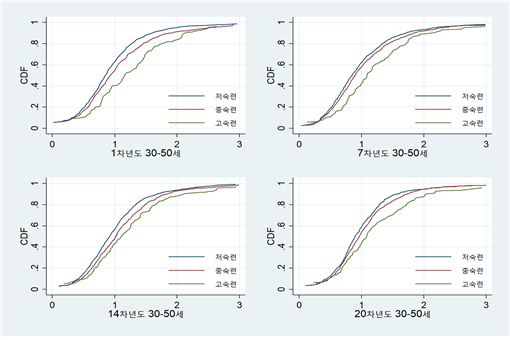
\includegraphics[scale=.7]{figure/klips_cdf4_byedu.png}
    \caption{가구소득의 누적분포: 가구주부친직업환경, 가구주연령 30-50세}
    \label{fig:klips_cdf4_byedu}
\end{figure}

각 년도의 누적분포는 환경수준이 높을수록 왼쪽에 위치하여 분명한 확률지배관계가 존재하는 것으로 보인다.
하지만 왼쪽 끝에 위치한 소득이 매우 낮은 가구들의 누적분포에서 환경수준 간 교차가 일어나는 것을 볼 수 있다.
따라서 모든 소득수준을 대상으로 하는 확률지배검증의 특성상 상이한 환경간의 확률지배가 없다는 결과를 도출할 가능성이 높다.
이러한 경향을 통제하기 위해 각 환경수준별 최하위 5 퍼센트와 최상위 5퍼센트를 제외한 가운데 90 퍼센트의 자료만으로 확률지배검증을 실시하였다.
 
\begin{figure}
    \centering
    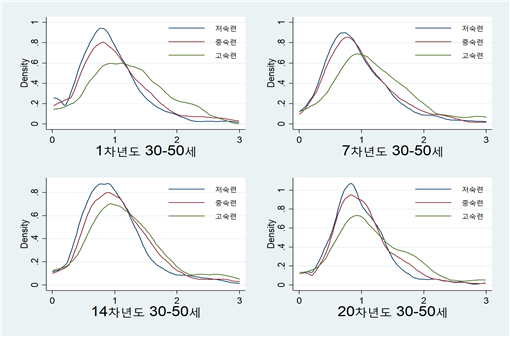
\includegraphics[scale=.7]{figure/klips_pdf4_byedu.png}
    \caption{가구소득의 확률분포: 가구주부친직업환경, 가구주연령 30-50세}
    \label{fig:klips_pdf4_byedu}
\end{figure}

매 조사년도에 연령이 가구주 연령이 30-50세인 가구들을 대상으로 확률지배 검증을 통해 기회불평등의 유무를 살펴보았다.
\footnote{모든 조사년도에 대한 확률지배 검증결과는 부록에 제시한다.}
그 결과 조사기간 전체에서 다수의 환경유형 쌍에서 확률지배관계가 존재하는 것으로 나타났다.
표 (\ref{tab:klips_dom_byjob})에 요약된 4개년도의 경우 총 12개의 환경유형 쌍 가운데 5개에서 확률지배 관계가 존재하는 것으로 나타났다.
1차년도와 20차년도에서 고숙련 집단이 다른 두 수준의 집단 모두를 확률지배 하여 기회불평등이 존재하였다.
전체년도로 확장하여 살펴보더라도 저숙련 집단과 중숙련 집단간에는 기회불평등이 존재하는 년도가 22개 년도 가운데 네 개 년도에 불과하지만 고숙련이 경우는 10이상의 조사년도에서 저숙련 집단이나 중숙련 집단에 대하여 2차 확률지배를 하여 기회불평등이 존재하는 것으로 나타난다.
그러나 다수의 열악한 환경이 우월한 환경을 확률지배 하는 경우는 전혀 없었다.

\begin{table}[htbp]
    \centering
    \caption{가구소득 누적분포의 확률지배 검증결과: 가구주부친직업환경, 가구주연령 30-50세}
    \resizebox{\textwidth}{!}{
\begin{tabular}{c|cc|cc|cc|cc}
    \hline \multirow{2}{*}{환경유형} & \multicolumn{2}{c|}{1차년도(1998)} & \multicolumn{2}{c}{7차년도(2004)} & \multicolumn{2}{|c|}{14차년도(2011)} & \multicolumn{2}{c}{20차년도(2017)} \\
    \cline{2-9} & 중숙련 & 고숙련 & 중숙련 & 고숙련 & 중숙련 & 고숙련  & 중숙련 & 고숙련  \\
    \hline 저숙련 & ? & $<_2^{***}$ & $<_2^{*}$  & ? & $<_2^{**}$  & ?  & ? & $<_2^{***}$ \\
    중숙련 & - & $<_2^{***}$ & - & ?  & - & ? & - & $<_2^{***}$ \\
    \hline
\end{tabular}}
    \confer{집단별 상하위 5\%를 각각 제외하고 검증. $=$ 은 동일한 확률분포, $<_{1}$은 행이 열에 1차 확률지배, $<_{2}$는 행이 열에 2차 확률지배 당하는 관계,  $?$는 확률지배관계를 확인 불가능한 경우임. ($*: \alpha = 0.5, **: \alpha = 0.01, ***: \alpha = 0.001$.)}
    \label{tab:klips_dom_byjob}
\end{table}

기회불평등 지수를 이용하여 연도별 기회불평등도의 추이를 분석한 결과는 그림 (\ref{fig:klips_jobgrp})와 같다.
먼저 기회불평등 전체의 추세를 알 수 있는 지니기회불평등지수부터 살펴본다.
가구주 연령을 30-50세로 제한 할 경우 전연령에 대상으로 하는 경우에 비하여 기회불평등 정도가 낮은 수준임을 알 수 있다.
반면 기회불평등 지수의 년도별 변동은 가구주 연령을 30-50세로 제한한 경우가 큰 것을 알 수 있다.
이는 앞서 언급한 바와 같이 연령을 통제하지 않은 경우에 환경변수의 비중이 변하면서 저수준집단이 고령화에 의한 소득감소의 효과를 받고, 고령자들은 은퇴이후 소득의 변동이 거의 없기 때문이다.
가구주 연령의 제한이 없는 경우  1998년부터 2006년까지는 기회불평등이 0.026 근처를 유지하는 모습을 보인다.
2007년부터 불평등 지수가 급상승 하여 2008년 이후는 평균 약 0.03의 수치를 보여 전후가 확연히 다른 모습을 보인다.
2017년부터 불평등 지수가 또 한번 가파른 상승을 하는네, 두 해 모두 노동패널 자료의 보충이 있었던 시기라는 공통점이 있다.

가구주의 연령을 30-50세로 제한하는 경우, 같은 기간동안 기회불평등도는 2007년 전후를 제외하고 0.02-0.026 사이에서 등락을 거듭하는 모습을 보인다.
COVID-19의 충격을 받은 2020년의 가구소득이 반영된 22회차에서 기회불평등 지수가 하락하는 모습을 보였다.
 
\begin{figure}
    \centering
    \caption{기회불평등지수 추이: 가구주부친직업환경}
    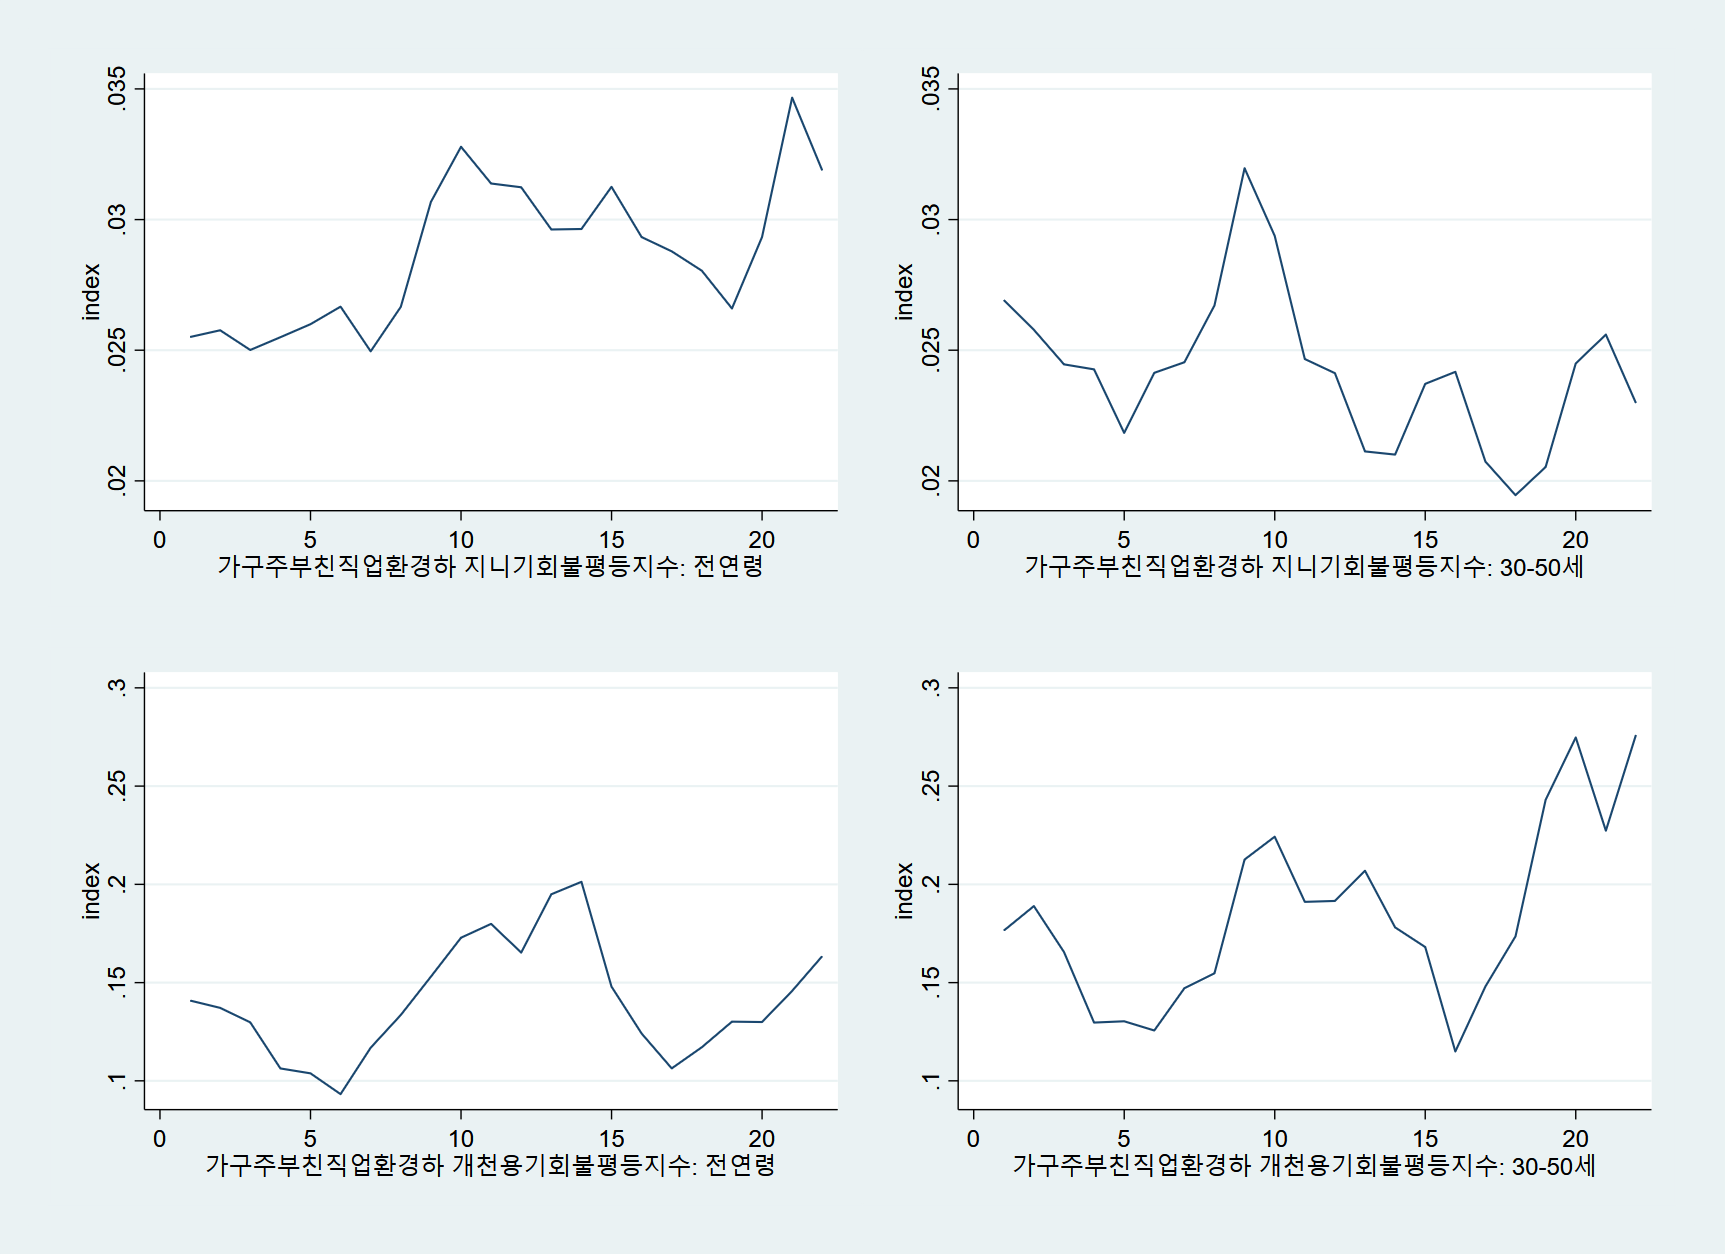
\includegraphics[width=\textwidth]{figure/incn1m_jobgrp_index.png}
    \label{fig:klips_jobgrp}
\end{figure}

개천용지수로 봤을 때 전연령과 30-50대의 기회불평등은 앞서와는 다른 모습이다.
가구주 연령을 제한하는 경우가 전연령을 대상으로 하는 경우보다 개천용 지수가 높게 나타나서 전반적인 기회불평등과 성공의 기회불평등이 상이함을 보이고 있다.
반면 연령대를 30-50으로 제한하는 경우 앞서와 마찬가지로 지수의 년도별 변동폭은 커짐을 알 수 있다.
특히 17차년인 2015년 이후부터 30-50세의 지수값과 전연령에서의 지수값의 격차가 크게 벌어지고 있다.
2020년 소득이 반영된 22회차 지수는 지니기회불평등 지수와는 다르게 전년도보다 상승하는 모습을 보였다.
우리 사회에서 체감하는 기회불평등에 대한 세대별 인식의 차이는 특히 소득상위 20\%와 같이 높은 수준의 성취를 대상으로 할 때 발생할 수 있음을 시사한다.

\subsection{가구주 부친 학력 환경}

가구주 부친의 교육 환경에 따라 얻어진 누적분포함수와 확률밀도함수를 각각 <그림 \ref{fig:klips_cdf4_byjob}>와 <그림 \ref{fig:klips_pdf4_byjob}>에 정리하였다.
가구주 부친의 직업을 환경변수로 했던 앞서의 결과와 마찬가지로 학력수준이 높은 집단일수록 누적분포가 아래에 위치하고 확률밀도가 오른쪽으로 치우치는 것을 볼 수 있다.

\begin{figure}
    \centering
    \caption{가구소득의 누적분포: 가구주부친직업환경, 가구주연령 30-50세}
    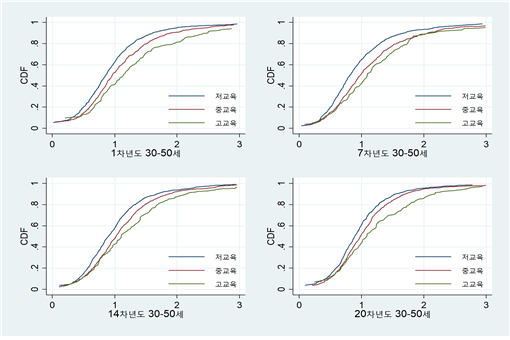
\includegraphics[scale=.7]{figure/klips_cdf4_byjob.png}
    \label{fig:klips_cdf4_byjob}
\end{figure}

\begin{figure}
    \centering
    \caption{가구소득의 확률분포: 가구주부친직업환경, 가구주연령 30-50세}
    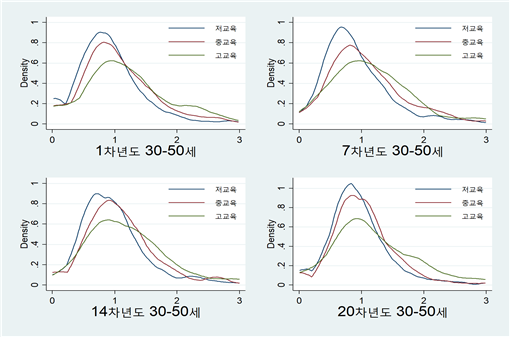
\includegraphics[scale=.7]{figure/klips_pdf4_byjob.png}
    \label{fig:klips_pdf4_byjob}
\end{figure}

확률지배 검증결과는 <표 \ref{tab:klips_dom_byedu}>과 같다.
4개의 조사년도 모두에서 고교육에 의한 저교육의 확률지배가 있어 특정집단간에 꾸준한 기회불평등이 있음을 알 수 있다.
학력환경하에서도 고교육 집단은 다른 집단들에게 확률지배 당하는 경우가 없어 기회불평등한 상황에 놓이지 않았다.
중교육집단 역시 저교육 집단에게 기회불평등한 년도는 없었다.

\begin{table}[htbp]
    \centering
    \caption{가구소득 누적분포의 확률지배 검증결과: 가구주부친학력환경, 가구주연령 30-50세}
    \resizebox{\textwidth}{!}{
\begin{tabular}{c|cc|cc|cc|cc}
    \hline & \multicolumn{2}{|c|}{1차년도(1998)} & \multicolumn{2}{c}{7차년도(2004)} & \multicolumn{2}{|c|}{14차년도(2011)} & \multicolumn{2}{c}{20차년도(2017)} \\
    \hline 환경수준 & 중교육 & 고교육 & 중교육 & 고교육 & 중교육 & 고교육  & 중교육 & 고교육  \\
    \hline 저교육 & ? & $<_2^{***}$ & $<_2^{**}$ & $<_2^{***}$ & $<_2^{*}$ & $<_2^{***}$ & $<_2^{**}$ & $<_2^{***}$ \\
    중교육 & - & $<_2^{**}$ & - & ?  & - & ? & - & ? \\
    \hline
\end{tabular}}
    \confer{집단별 상하위 5\%를 각각 제외하고 검증. $=$ 은 동일한 확률분포, $<_{1}$은 행이 열에 1차 확률지배, $<_{2}$는 행이 열에 2차 확률지배 당하는 관계,  $?$는 확률지배관계를 확인 불가능한 경우임. ($*: \alpha = 0.5, **: \alpha = 0.01, ***: \alpha = 0.001$.)}
    \label{tab:klips_dom_byedu}
\end{table}

지수를 이용한 가구주부친학력환경하 기회불평등의 추이는 <그림 \ref{fig:klips_edugrp}> 과 같다.
먼저 지니기회불평등지수를 앞서의 직업환경하에서 도출한 수치들과 비교한다.
가구주 부친의 학력을 환경으로 하는 경우 직업을 환경으로 하는 경우보다 0.005 높은 기회불평등 수치를 보이고 있다.

전연령의 경우 직업환경하에서 나타났던 2007년경의 기회불평등 상승 추세는 관찰되지 않는다. 
하지만 2016년의 기회불평등 상승은 앞서와 같은 양상이지만 더 높은 수치로 나타나고 있다.
30-50세 집단은 5차년도인 2002년 부터 2016년 까지 기회불평등이 꾸준히 감소하는 모습을 보이지만 여전히 직업환경 하의 수치들 보다는 높다.

\begin{figure}
    \centering
    \caption{기회불평등지수 추이: 가구주부친학력환경}
    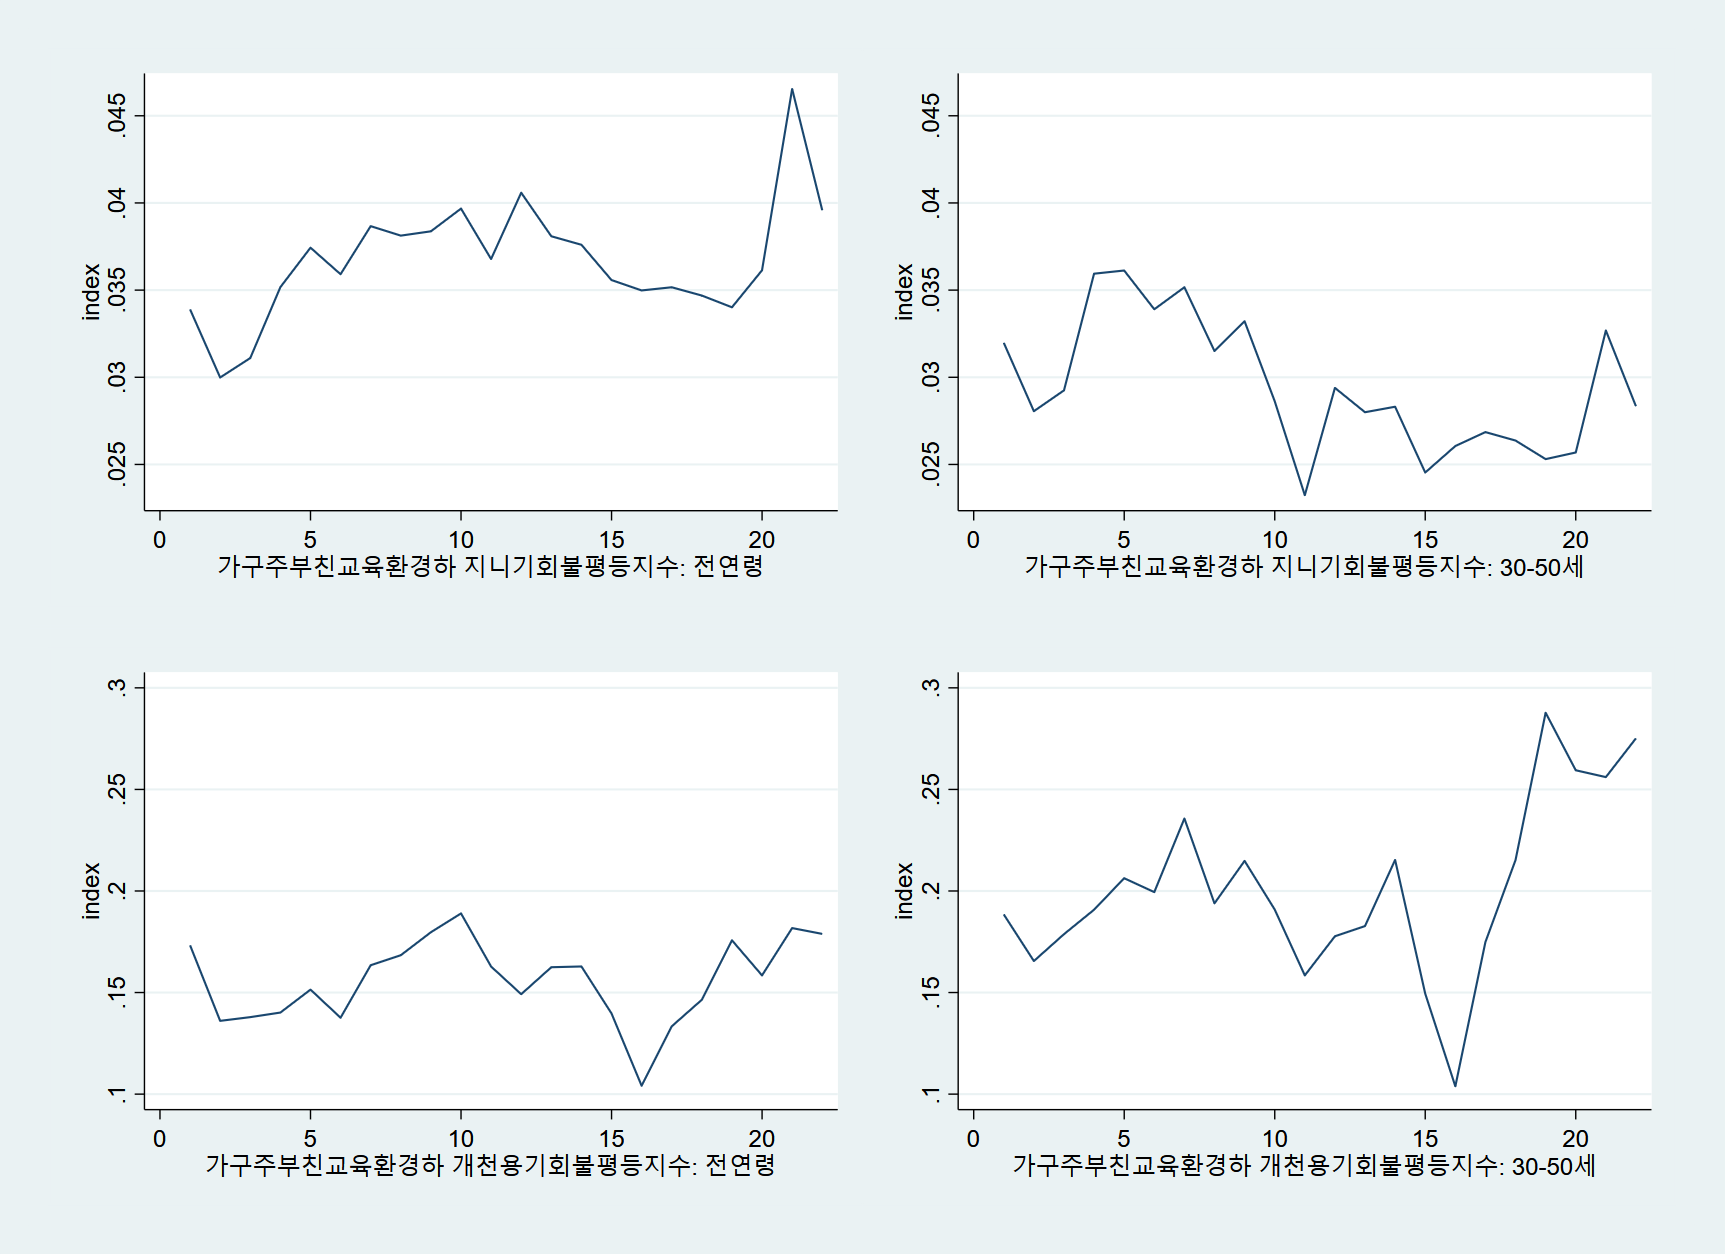
\includegraphics[width=\textwidth]{figure/incn1m_edugrp_index.png}
    \label{fig:klips_edugrp}
\end{figure}

개천용기회불평등지수의 경우 지니기회불평등지수와는 다르게 직업환경과 학력환경에서 지수값 차이가 거의 없다.
30-50세 집단의 경우 17년차인 2015년 이후 기회불평등 수치의 급격한 상승을 보이고 있다.
이 추세는 앞선 직업환경하에서 나타나는 모습과 동일하여 지니기회불평등 지수의 추세가 가구주 연령의 제한여부에 따라 다른 양상을 보이는 것과 구분된다.

\section{미국과 유럽 연구결과와의 비교}

\citet{letl08}는 90년대 초반 유럽 전역의 8개국과 미국의 소득자료를 이용하여 가구주 부친의 학력을 환경변수로 하여 세 가지 환경수준으로 구분하고 확률지배검증을 통한 기회불평등 존재유무 검증과 지니기회불평등지수 계산을 수행하였다.
 그 가운데 일부 내용을 소개하여 한국과 비교하고자 한다.
 
\begin{figure}
    \centering
    \caption{스웨덴, 노르웨이, 이탈리아, 미국의 가계소득 누적분포: 가구주부친 학력환경}
    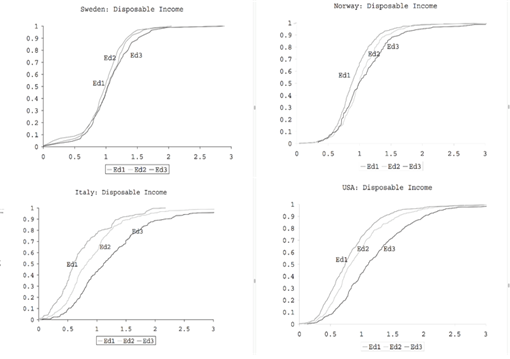
\includegraphics[width=\textwidth]{figure/letl08.png}
    \source{\citet{letl08}}
    \confer{Ed1: 저교육, Ed2: 중교육, Ed3: 고교육.}
    \label{fig:letl08}
\end{figure}

<그림 \ref{fig:letl08}>은 스웨덴, 노르웨이, 이탈리아, 미국 4개국의 1990년대 초·중반에 측정된 가구주 부친의 학력을 환경변수로 한 환경수준별 누적밀도분포이다.
 먼저 위 열의 두 그림과 아래 열의 두 그림이 확연한 차이를 보이는 것을 알 수 있다.
 스웨덴의 경우 환경수준별 누적분포의 간격이 거의 없이 일치하는 것을 볼 수 있고, 노르웨이도 중학력(Ed2)과 고학력(Ed3) 집단간의 누적분포가 거의 차이가 없는 것을 알 수 있다.
 반면, 아래의 이탈리아와 미국은 <그림 5>에서 한국의 1998년 경우보다 환경수준별 누적밀도분포의 간격이 더 큰 것을 알 수 있다.

이러한 결과는 확률지배검증의 결과로도 확인되는데 스웨덴은 놀랍게도 가처분소득 기준으로 기회평등을 달성한 것으로 나온다.
 반면 이탈리아와 미국의 경우는 모든 환경수준의 쌍에서 2차 확률지배관계가 있는 것으로 나오는데 분포의 양 끝 5\% 제외한 우리의 검증결과에 대입해 보면 모두 1차 확률지배관계로 나올 것으로 생각할 수 있다.
 
 \begin{table}[htbp]
     \centering
     \caption{국가별 지니기회불평등지수 비교}
     \begin{tabular}{c|c|c|c}
\hline 국가 & 자료년도 & 지수값 & 표준편차 \\
\hline 한국$^{*}$ & 1998 & $3.19$ & $0.780$ \\
\hline 스웨덴$^{***}$ & 1991 & $1.09$ & $0.606$ \\
\hline 노르웨이$^{***}$ & 1995 & $2.18$ & $0.581$ \\
\hline 이탈리아$^{***}$ & 1993 & $7.64$ & $0.531$ \\
\hline 미국$^{***}$ & 1991 & $6.93$ & $0.586$ \\
\hline 독일$(서독)^{**}$ & 1994 & $0.88$ & $0.426$ \\
\hline 영국$^{***}$ & 1991 & $3.45$ & $0.683$ \\
\hline 프랑스$^{*}$ & 1994 & $4.22$ & $0.406$ \\
\hline 벨기에$^{***}$ & 1992 & $4.58$ & $0.581$ \\
\hline
\end{tabular}
     \\
     \source{한국을 제외한 수치는 \citet{letl08}.}
     \confer{가구주연령대는 *:30-50세, **:25-45세,  ***25-50세.}
     \label{tab:klips_letl08}
 \end{table}

표 \ref{tab:klips_letl08} 는 한국과 \citet{letl08}에서 계산된 지니기회불평등지수의 값을 나열한 자료이다. 스웨덴, 노르웨이의 지수 값은 각각 1.09와 2.18로 이탈리아 미국의 7.64와 6.93에 비해 훨씬 낮은 수치이다. 비록 한국의 자료조사연도가 나머지 국가에 비해 늦기 때문에 비슷한 시점에서의 비교라고 할 수는 없겠지만 그 정도는 영국, 프랑스 벨기에 등과 비슷하며 이탈리아, 미국보다는 기회불평등 정도가 낮은 것으로 나온다.

\section{소결론 및 시사점}
가구주의 환경별로 가구들의 가처분소득 확률분포를 도출하고 이러한 분포들 사이의 확률지배관계로 정의되는 기회불평등의 유무를 검증하고 기회불평등도를 분석하였다.
 가구주 부친의 직업과 학력이라는 두 가지 환경변수를 활용하여 기회불평등의 존재 여부를 살펴본바, 두 환경 모두에서 기회불평등이 존재하는 것으로 나타났고 가장 높은 수준의 환경집단은 나머지 집단을 거의 모든 경우에 확률지배하는 것을 알 수 있었다.
 
지니기회불평등지수와 개천용 지수를 이용한 기회불평등도를 분석한 바, 학력을 환경변수로 사용하는 경우가 직업을 사용하는 경우에 비해 기회불평등도가 더 큰 것을 알 수 있었다.
 지니 기회불평등지수의 경우 가구주의 연령대를 제한할 경우 제한하지 않을 때보다 불평등 정도가 크게 내려갔다.
 이는 과거 빠른 경제성장의 효과로 인한 교육기회의 양적 증가와 산업구조의 고도화 결과 우리가 환경으로 생각하는 변수들이 크게 변했고, 따라서 은퇴 등으로 인해 소득이 많이 감소하는 고연령층일수록 열악한 환경에 처한 가구의 비중이 크기 때문이다.
 또한, 나이를 제한하는 경우 지수값이 일정한 추세를 나타내는 것 역시 환경의 변동을 나이 제한으로 통제한 결과로 볼 수 있다.
 가구주의 나이를 30-50세로 제한한 경우 최근 년의 개천용지수가 급상승하는데 이는 우리 사회가 체감하는 높은 기회불평등은 주요경제활동연령층이 경제적 성공을 얻는 데 대한 기회불평등임을 보여주고 있다.

향후 연구과제는 다음과 같다.
먼저 기회불평등을 없애는데 필요한 최소한의 부의 이전을 생각해 볼 수 있다.
우리의 연구방법에서 기회불평등은 확률지배검증의 결과인데 그렇다면 확룰지배가 일어나지 않게 누적분포가 서로 교차할 수 있게 하는 환경수준 간 피구-달튼 형태의 소득 이전을 하나의 예시로 생각해볼 수 있다.
이를 통해 기회불평등 해소를 위한 최소한의 재분배정책의 규모를 가늠해볼 수 있다.
다음으로 경제위기가 기회불평등에 주는 영향에 대하 알아볼 필요성이 제기된다.
COVID-19로 시작된 경제위기가 우리 사회의 소득의 기회불평등에 어떤 영향을 주는지에 대한 구체적인 연구가 진행되어야 할 것이다. 현재는 2020년 한 해의 소득자료만 관찰 가능 하지만 자료가 추가되는 2-3년 이내에 구체적인 연구가 가능할 것으로 생각된다.

\chapter{기회불평등과 경제성장}
\section{들어가는 말}
\label{ans4}
 한 경제의 불평등 정도와 경제성장의 사이의 관계는 많은 경제학 연구의 관심 대상이 되어 왔다. 최근 전 세계 국가들의 경제성장이 둔화되고 경제적 불평등이 심화되면서 불평등이 경제성장에 미치는 영향에 대한 관심이 보다 높아지고 있다.
 
경제적 불평등과 경제성장 사이의 관계에 대한 연구는 1990년대부터 본격적으로 시작되어 약 30여 년간 끊임없이 진행되었다.  다수의 연구가 장기에는 높은 불평등이 경제성장에 부정적인 영향을 준다는데 대한 합의가 있지만, 단기간을 살펴봤을때 아직 이들 두 변수 사이의 관계에 대해 확정적인 결론은 도출되지 않고 있다.

불평등과 경제성장 간의 관계에 대한 주요 이론은 크게 두 가지로 나눌 수 있다. 첫번째는 불평등한 소득분포가 자본 시장의 불완전성(markek imperfection)과 결합하여 경제성장의 위한 효율적인 인적자본 축적을 저해한다는 내용이다(\citet{gnz93}; \citet{loury81}). 예를들어 개인이 고등교육과 경제활동참여 사이에 진로선택을 해야하는 상황에 놓인다고 하자. 만약 자본시장에 불완전성이 존재한다면 충분한 능력과 의욕이 있는 개인이라 할지라도 자금조달을 못해 고등교육 진학이 더 효율적임에도 당장의 경제활동 참여를 시작할 수 밖에 없다. 경제적 불평등의 증가는 이러한 개인들의 수의 증가로 이어져 경제 전체에서는 비효율성이 증가할 것이고, 결국 경제적 불평등이 경제성장을 저해하는 결과로 이어진다.

불평등과 경제성장에 대한 두번째 주요이론은 불평등이 정책 선택(policy decision)에 영향을 주고 이러한 정책이 경제성장에 영향을 준다는 것이다(\citet{anr94}; \citet{pnt94}).  이들의 이론에 따르면, 정책 결정은 중위투표자(median voter) 모형에 근거하여 이들 중위투표자의 선호에 가깝게 결정된다. 경제적 불평등이 심화되면 중위투표자의 소득과 평균소득(mean income)의 차이가 확대되고 이런 상황에서 중위투표자는 소득재분배 기능을 강화하여 자신의 소득 상승시키는 정책을 선호하게 된다. 과도한 재분배 정책은 지나치게 높은 세율을 수반하여 결국 경제성장을 저해한다는 것이다.

불평등이 경제성장에 미치는 영향을 다룬 초기의 실증연구들은 대개 국가단위 횡단면(cross-national) 자료를 이용해 소득불평등이 경제성장에 부정적인 영향을 미친다고 주장하였다(\citet{barro91}; \citet{anr94}; \citet{pnt94}). 반면, 2000년대 이후에는 다수의 학자들이 이전 연구들의 한계를 지적하면서 국가별 패널자료를 활용하여, 불평등과 경제성장 사이에는 양(positive)의 관계가 존재하기도 하고, 대체로 강건한 추정결과가 잘 도출되지 않는다는 결론을 제시한다(\citet{lnz98}; \citet{barro20}; \citet{forbes00}; \citet{bnd03}).

최근에는 이와 같이 연구 결과가 상이하게 나타나는 원인에 대한 분석과 그 원인을 고려한 새로운 접근법이 시도되고 있다. 국가별 패널 분석의 결과가 확정적이지 않은 이유를 밝히기 위해 최근의 연구들은 불평등의 효과가 국가들 사이에 이질적일 가능성, 불평등을 구성하는 각 요인이 경제성장에 미치는 효과가 이질적인 가능성 등을 고려하고 있다(\citet{voit05, voit11}; \citet{cc10}; \citet{hetl14}; \citet{mnr13,mnr14}). 이들 중 한 부류의 연구에서는 기존 연구에서 사용한 불평등은 성과(achievement)의 불평등으로서, 성과의 불평등은 그 원인에 따라 각각 기회의 불평등(inequality of opportunity)과 노력의 불평등(inequality of effort)으로 분해될 수 있다고 제안한다. 이들은 기회의 불평등과 노력의 불평등 각각이 경제성장에 서로 상반되는 영향을 미치는 경우, 단일 지표인 성과의 불평등이 경제성장에 미치는 효과는 일관되게 나타나지 않을 수 있다고 지적한다(\citet{mnr13, mnr14}; \citet{metl13}; \citet{fetl18}; \citet{ane20} ).

\citet{kno17}는 \citet{mnr13}의 연구방법을 확장하여 기회의 불평등이 경제성장에 주는 영향을 연구하였다. 기회불평등과 경제성장 사이의 관계를 실증적으로 추정하기 위해 통계 분석의 단위를 한 국가 내의 서로 다른 지역들이 아니라 전 세계의 서로 다른 국가들로 확장하였다. 이를 위해 국제교육평가 자료인 TIMSS를 이용하여 70여개 국가를 대상으로 교육의 기회불평등과 노력불평등을 측정한 비대칭 패널 자료를 구성하고 이를 거시경제 변수와 결합하였다. 기존의 연구에서 불평등과 경제성장률 간의 관계가 불분명한 것은 기회와 노력의 불평등이 서로 상반된 방향으로 작용했기 때문이며 특히 OCED 국가와 같은 일정수준의 경제발전이 이루어진 국가들에서 이러한 혼재된 관계가 분명함을 보였다.

본 연구는 \citet{kno17}의 연구를 두 가지 측면에서 확장한다. 첫째, 또 다른 교육평가 자료인 PISA를 더하여 관찰 가능한 자료의 수를 확장한다. 한 국가의 서로 다른 시점 별로 기회의 불평등도와 노력의 불평등도를 측정하기 위해 전 세계의 초$\cdot$중$\cdot$고등학생들을 대상으로 실시되는 국제 교육성취도 평가인 TIMSS(Trends in International Mathematics and Science Study)와 PISA(Programme for International Student Assessment)의 성적 자료를 사용한다. 둘째, \citet{betl12}에서 제시한 기회불평등 측정의 개선 방안을 도입하여 기회불평등의 개념에 보다 더 가까운 지수를 이용한다. 기회불평등 측정이 일반적으로 가지는 기호의 불평등 과소측정의 문제를 계량경제학적 기법으로 개선하여 합리적인 동시에 덜 엄격한 기회불평등 정도를 추정한다.   이렇게 도출된 국가별 교육의 기회불평등도와 노력불평등도를 여러 시점에 측정하고, 이들 불평등지수를 각국의 경제성장률과 연결시킴으로써 각 유형의 불평등이 일국의 경제성장에 미치는 영향을 실증적으로 분석한다. 이를 통해 우리는 불평등이 경제성장에 미치는 영향을 보다 세부적으로 규명하고자 한다.

\label{ans5-1}
본 연구는 교육성취에서 기회의 불평등과 노력의 불평등을 해당 국가의 노력에 대한 보상이 얼마나 잘 이루어 지는가에 대한 대리변수로 간주한다.
결과의 불평등이 개인의 의지나 노력과 무관한 환경에 의해 크게 좌우된다면 필연적으로 개인들이 성취의을 감소시키고 이는 사회 전반의 생산성 저하로 이어질 것이다.
교육성취의 경우 청소년을 대상으로 측정하기 때문에 가정이나 사회와 같은 환경의 영향이 더욱 분명하게 드러나고, 현재의 성취가 과거 본인의 노력이나 환경의 영향을 덜 받는다는 점에서 의의가 있다.

본 장은 이하에서 다음과 같이 구성된다.
제2절에서는 불평등과 경제성장 사이의 관계를 분석한 선행 연구들을 정리한다.
제3절에서는 실증분석 방법을 자세하게 설명하고, 제4절에서는 주요 분석결과를 정리한다.
제5절에서는 4절의 결과에 대한 강건성을 검증하고, 마지막 6절에서 글을 끝맺음 한다.

\section{선행 연구}
\subsection{불평등과 경제성장}
경제 내 불평등과 경제성장 사이의 관계를 다룬 초기의 연구들은 주로 국가 단위의 횡단면 자료를 사용하였다(\citet{barro91}; \citet{anr94}; \citet{pnt94}).
이러한 분석방법은 국가들 사이에 존재하는 이질성을 적절히 통제할 수 없기 때문에 이후의 연구들은 국가별 패널 자료를 이용해 불평등이 경제성장에 미치는 영향을 분석하였다(\citet{lnz98}; \citet{barro20}; \citet{forbes00}; \citet{bnd03}).
국가별 패널 자료를 이용한 연구들은 불평등이 경제성장에 부의 효과, 양의 효과, 0의 효과 등 매우 혼재된 추정치를 제공한다.
그에 따라 불평등과 경제성장 사이의 관계에 대한 확정적인 결론이 도출되지 못하고 있다.

패널분석의 결과가 이처럼 혼재되어 나타나는 이유를 밝히기 위해 최근의 연구들은 불평등의 효과가 국가들 사이에 이질적일 가능성, 불평등을 구성하는 각 요인이 경제성장에 미치는 효과가 이질적인 가능성 등을 고려하고 있다.
\citet{voit05, voit11}는 한 경제의 불평등도를 측정할 때 사용하는 소득의 분포에서 상위 소득에서의 불평등이 경제성장에 미치는 영향과 하위 소득에서의 불평등이 경제성장에 미치는 영향이 서로 상이할 가능성을 제기하였다.
그의 실증분석에 의하면, 개별 국가 소득분포의 최상위층에서의 불평등은 경제성장과 양의 관계를 보인 반면, 하위층에서의 불평등은 음의 관계를 갖는다.
즉 전체 소득분포를 하나의 불평등지수로 단일화시켜 분석한 기존 연구에서는 이들 두 효과가 혼합되어 있다.
\citet{voit05, voit11} 이후의 많은 연구들은 불평등의 이질적인 효과를 구분하기 위해 분석 대상 국가의 특성, 소득수준 및 영향을 미치는 기간 등을 명시적으로 고려한다.

\citet{cc10}는 불평등과 경제성장 간의 관계가 개별 경제의 소득수준에 따라 상이할 가능성을 고려하면서 국가별 패널자료를 분석하였다.
그는 저$\cdot$중소득 경제에서는 불평등이 경제성장에 부정적인 영향을 미치는 반면, 고소득 경제에서는 경제성장에 긍정적인 영향을 미친다는 점을 발견하였다.
\citet{hetl14}은 불평등도와 경제성장의 관계에서 시간에 주목했는데, 그들은 단기에는 이들 사이에 양의 관계가 존재하지만 반대로 장기에는 양의 관계가 존재함을 발견하였다.

\citet{nns13}와 \citet{nns16}는 기존의 연구들에 대한 메타분석(meta analysis)을 통해 각 논문에서 사용한 자료의 구조와 분석 대상 국가들의 성격, 지역 더미변수의 포함여부, 불평등의 정의 및 소득의 정의에 따라 각 논문이 제시한 불평등의 효과가 서로 매우 이질적임을 보였다.
불평등과 경제성장 사이의 관계는 선진국과 개발도상국에서 서로 상이하여, 개도국에서는 두 변수 사이에 음의 관계가 나타나는 반면 선진국은 유의하지 않거나 양의 관계가 나타날 수 있다고 주장하였다.
\citet{cetl21}은 30여년간 출간된 불평등과 경제성장간의 관계에 대한 논문 총 36건을 조사하였다.
30년 이상의 장기에는 이들의 관계가 서로 부정적이라는 점에 대한 합의가 있는 반면에 10년 이하의 단기간에는 상호 긍정적, 부정적, 무관계 등의 관계가 연구마다 상이하게 나오는 것으로 집계하였다.

\begin{figure}
    \centering
    \caption{불평등, 빈곤, 경제성장간의 연구결과 정리}
    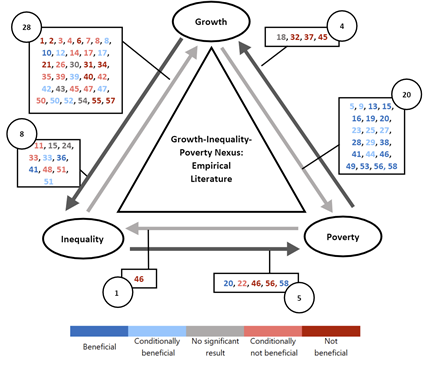
\includegraphics[width=\textwidth]{figure/triangle_relations.png}
    \source{\citet{cetl21}}
    \label{fig:triangle relations}
\end{figure}

경제성장과 불평등의 관계에 대한 연구에서 기회불평등의 개념의 도입은 비교적 최근에 이루어 졌다.
\citet{mnr13, mnr14}는 각각 미국과 전 세계를 대상으로 기회불평등과 경제성장 간의 관계를 연구했는데 노력의 불평등과 경제성장의 관계는 유의하지 않지만, 기회의 불평등과 경제성장 사이에는 분명한 음의 관계가 있음을 발견하였다.
\citet{metl13}은 농경자본을 도구변수로 사용해 교육의 기회불평등을 측정하고, 기회불평등과 경제성장 사이에 음의 관계가 있다고 주장한다.

\citet{mnr13}은 미국의 50개 주를 대상으로 각 주별로 개인 소득의 총불평등을 기회불평등과 노력불평등으로 분해한 패널 자료를 구성하고, 이들 두 변수를 주별 경제성장률과 연결시켰다.
이들은 기회의 불평등과 노력의 불평등이 경제성장에 각각 음과 양의 상반된 영향을 미침을 보임으로써, 선행 연구에서 도출되는 불평등과 경제성장 사이의 모호한 관계가 기회불평등과 노력불평등 각각이 경제성장에 미치는 효과가 서로 상반되기 때문이라고 주장하였다.
\citet{mnr13}의 연구는 불평등과 경제성장 연구의 범위를 확장하면서 불평등이 성장에 미치는 보다 자세한 메커니즘을 분석한다는 점에서 의미 있는 기여를 하고 있다.
그러나 그들은 미국 내의 50개 주를 대상으로 분석하고 있기 때문에, 이 연구로부터 도출된 결과의 해석은 제한적일 수 있다.
첫째, 분석대상인 미국의 주 간에 사람들의 자유로운 이동이 가능하므로 기회의 불평등이 낮은 지역으로 사람들이 이주하는 내생성이 존재할 수 있다.
둘쩨, 경제성장과 불평등간의 관계에서 관심 단위는 주로 국가라는 점에서 한 국가내의 서로 다른 지역을 대상으로 한 연구의 결과를 직접 젹용하기 어렵다.

 \citet{fetl18}는 전세계 42개국에서 117개의 가구조사와 134개의 인구통계학적 건강조사 자료를 취합해 각국의 불평등도를 1985년부터 2005년까지 5년 간격으로 측정하여 소득의 불평등에서 기회의 불평등이 차지하는 비중이 약 5-13 퍼센트라고 보고한다.
 그들의 분석결과에 의하면, 경제성장과 기회의 불평등 사이에는 음의 관계가 나타났지만 그 결과는 그리 강건하지 못하다.
\citet{fetl18}은 \citet{mnr13}에서 도입된 기회불평등과 경제성장간의 관계에 대한 연구를 국가단위로 확장시켰고, 다양한 국가에서 소득 및 건강의 기회불평등을 측정했다는데 의의가 있다.
 또한 불평등이 경제성장에 부정적 영향을 준다는 주장에 대한 반론을 제기하는 최소한의 근거를 제시하였다.
 그러나 그들의 연구에서 사용한 환경에는 기회불평등 문헌에서 중요한 환경 요인으로 간주하는 ‘부모의 능력 변수(부모의 학력, 소득, 재산 등)’가 제외되어 있다.
 
\citet{ane20}는 기회불평등 개념을 경제성장괴 불평등간의 관계에 도입한 가장 최신의 실증연구이다.
이 연구는 총 111개국을 대상으로 하여 불평등의 척도로 각 국가의 소득의 지니계수를 사용하였다.
세대간 소득 또는 교육탄력성을 기회불평등의 척도로 활용하였고, 기회불평등의 정도가 높을 수록 소득불평등이 경제성장에 부정적 영향을 주는 것을 확인하였다. 
\citet{ane20}는 국가간 종단자료를 이용하여 기회불평등과 경제성장 간의 유의미한 부정적 관계를 확인한 연구이다.
그러나 \citet{corak13}의 지적과 같이, 비슷한 수준의 세대간 탄력성이 측정되는 집단들 간에도 기회불평등은 큰 차이가 있을 수 있다.
따라서 이 연구는 기회불평등의 개념을 도입했지만 기회불평등 지수를 사용하지 않았다.


\subsection{기회불평등}

경제학에서 불평등에 관한 연구는 소득, 교육수준, 건강과 같이 인간이 이루는 성취의 불평등에 대하여 그 윈인을 고려한 기회의 불평등(Inequality of Opportunity)으로 그 연구범위가 확장되고 있다.
기회불평등의 개념은 평등주의 철학자들로부터 먼저 연구되었는데, 이들은 한 사회에서 구성원들이 만들어 내는 성취의 불평등이 각 개인의 순수한 의지와 무관한 요소에 의해 발생한다면 이것은 도덕적으로 정당화 할 수 없고, 따라서 사회는 이러한 불평등을 제거하는데 힘써야 한다고 주장한다.
예를 들어, 학생의 학업성취도를 부모의 경제력과 학생 본인의 노력의 함수라고 가정하면, 학업성취도의 총불평등은 부모의 경제력 차이에 기인하는 불평등과 본인 노력의 차이에 기인하는 불평등으로 분해될 수 있다.
이때 부모의 경제력 차이는 환경(혹은 기회) 요인으로서 학생 개인에게 그 책임을 지을 수 없기 때문에, 환경의 차이로부터 발생하는 학업성취도의 불평등은 정당화되기 어렵고 이를 줄이거나 없애기 위해 노력해야 한다.

기회불평등에 대한 본격적인 연구는 \citet{Rawls99}로부터 시작되었다.
 그는 개인의 성취를 노력, 환경, 그리고 운이 복합적으로 작용한 결과라고 말한다.
 그에 의하면 성취의 불평등은 그 원인에 따라 개인에게 책임을 귀속시킬 수 있는 부분과 책임을 귀속시킬 수 없는 부분으로 나뉠 수 있다.
 노력의 차이에 의해 발생하는 불평등에 대해서는 마땅히 그 개인이 책임져야 하겠지만, 개인의 의지와 무관하게 주어지는 환경의 차이에 따른 불평등은 도덕적으로 정당화하기 어렵다.
 
롤즈의 평등사상은 현대적 의미로 개인에게 “동등한 출발선” 또는 “기울어지지 않은 운동장”을 보장해야 한다는 개념으로서, 그는 이러한 “공정한 기회”의 제공을 위하여 실질적인 기회평등이 필요하다고 보았다.
동일한 천부적 능력과 야망을 가진 사람들에게는 그 사람의 가정환경, 상속된 부의 크기, 인종, 성 등과 무관하게 동등한 성취의 전망(prospects of success)이 보장되어야만 한다는 것이다.
\footnote{\citet{Rawls99}, p.63.}

기회평등의 원칙은 드워킨(Ronald Dworkin), 아네슨(Richard Arneson), 코헨(Gerald. A. Cohen) 등의 정치철학자들에 의하여 꾸준히 연구가 진행되었고, \citet{Roemer98}에 이르러 비로소 경제학에 적용가능한 개념으로 정립되었다.
\citet{Roemer98} 이후 많은 경제학 연구들이 기회불평등 개념을 실증분석에 적용하고 있다.
\footnote{기회불평등을 다룬 경제학 연구들은 \citet{rnv12}, \citet{fnp15}, \citet{rnt16}에 잘 정리되어 있다.}
본 연구는 이들 연구에서 성취의 불평등도를 기회의 불평등도과 노력의 불평등도로 분해하는 방법을 차용해 불평등의 두 구성요소 각각이 한 국가의 경제성장에 미치는 영향을 실증적으로 분석한다.

\section{실증분석 방법}

본 연구는 \citet{kno17}의 연구를 자료와 불평등 지수 두 부분에서 확장한다.
자료 측면에서 기존연구가 기회불평등 측정을 위해 사용한 TIMSS 이외에 또 다른 국제교육평가 자료인 PISA를 사용한다. TIMSS만을 사용할 경우 1995년부터 2019년 가운데 총 7개 년도에 대한 기회불평등 측정이 가능하고 그 가운데 경제성장과의 관계를 분석하는데는 최대 6개 년도의 자료를 활용 할 수 있다. PISA를 추가적으로 연구하여 2000년부터 2018년 가운데 5개 년도의 시점에 대한 불평등 측정이 추가되고 특히 2003, 2015년은 두 자료가 모두 생성되에 두 자료의 차이점에 대한 비교 연구 역시 진행할 수 있다.

기회불평등의 측정에 있어 \citet{betl12}에서 제시한 개선점을 활용한다.
교육성취인 시험점수를 기여요인에 따라 환경으로 인한 기회의 불평등과 그 밖의 요인에 의한 잔여불평등으로 구분하여 측정한다.
그후 잔여불평등에서 직접 관찰할 수 없지만 환경의 영향을 받은 요인을 분리하여 노력불평등을 측정한다.

먼저, 기회의 불평등은 대체로 경제성장에 부정적인 영향을 미칠 가능성이 높다.
기회의 불평등이 존재하는 경우, 보다 우월한 노력을 투입한 사람들보다는 우월한 출신배경을 가진 사람들이 인적자본을 축적하기에 유리한 환경이 조성되고, 개인들의 노력이 경제 내에서 적절한 보상을 받지 못할 수 있기 때문이다.
반면, 노력의 불평등은 경제성장에 긍정적인 영향을 미칠 가능성이 높다.
상이한 노력을 투입한 사람들 사이의 소득불평등은 상이한 노력에 대한 보상을 반영하기 때문에, 노력의 불평등은 사람들이 더 많은 노력을 투입할 유인을 제공하기 때문이다.
기존의 실증연구에서 불평등이 경제성장에 미치는 영향이 확정적인 방향으로 도출되지 않는 이유 중 하나는 기회의 불평등과 노력의 불평등 각각이 경제성장에 미치는 효과가 서로 상반되기 때문이다.

본 연구에서는 중학생들의 학업성취도를 이용해 불평등을 측정하기 때문에, 본 연구가 분석하는 불평등의 효과는 엄밀하게는 경제적 불평등의 효과가 아니라 교육성취도의 불평등의 효과이다.
일반적으로 경제적 불평등은 교육성취도의 불평등과 전반적인 경제 구조로부터 발생하는 불평등이 결합되어 있으므로 본 연구에서는 경제적 불평등이 경제성장에 미치는 전체 효과의 일부분만을 분석하고 있다.
이러한 한계점은 여러 국가들을 대상으로 기회불평등과 노력불평등을 측정해야 하는 실증적인 어려움으로부터 발생한다.

본 연구에서는 불평등을 경제성장과 연결시키기 때문에 경제성장을 표현하는 자료들 또한 필요하다.
우리는 선행 연구들을 따라 Penn World Tables(PWT)을 이용해 각 국가의 시점별 1인당 GDP 및 기타 거시자료들을 구축한다.
PWT는 183개국에 대해 1950년부터 2019년까지의 인구, 실질총생산, 물가수준, 고정자본수준 등 방대한 거시자료를 축적한 데이터베이스 이다.
TIMSS와 PISA의 조사대상인 98개국의 거시자료 역시 PWT에 포함되어 있다.

\subsection{불평등지수의 계산}
우리는 \citet{mnr13}의 연구방법을 따라 TIMSS와 PISA의 국가별 각 시점 자료에 대해 아래와 같은 방법을 적용해 학업성취도의 총불평등도과 그것을 분해한 기회불평등도 및 잔여불평등도를 측정한다. 

개인 $i$가 $N$명으로 구성되어 있는 어떤 사회의 한 구성원이라고 가정하자$(i \in \{1,\ldots,N \} )$.
개인 $i$가 속하는 환경변수 $C_{ic}$는 개인의 성취에 영향을 주면서 그 개인이 스스로의 의지로 선택할 수 없는 요인이다.
환경변수는 부모의 학력, 출생지의 규모, 부모의 소득, 인종, 성별 등 실제 자료에서 쉽게 관찰할 수 있는 다양한 요소가 될 수 있다.
개인 $i$가 속하는 환경 $C_i$는 이러한 환경변수$C_{ic}$ 들의 c-터플(c-turple) $C_i = \{C_{1i}, \ldots , C_{ci}\}$이다. 
환경유형 $T= \{1, \ldots , t \}$, $t= ||C_1|| \times \cdots \times ||C_c||$는 편의를 위하여 가능한 환경의 집합 $\{ C_i \}$을 정의역으로 취하는 지표(index)이다.

개인의 학업성취도를 $y_i$, 개인이 속한 환경유형을 $T_i$, 개인이 하는 노력을 $e_i$라고 표시하자.
기회불평등의 관점에서 성취는 개인이 속한 환경 및 환경과 무관한 개인의 노력의 결과라고 정의한다.
이때 성취 $y_i$의 확률밀도함수 $f(\cdot)$는 $ y_i = f(T_i, e_i)$와 같이 표시할 수 있다.

본 연구에서 계산하는 기회불평등 지수는 \citet{fng11}에서 제시한 방법에서 출발한다.
타일-0 지수(Theil-0 index)는 지니계수 이외의 방식으로 불평등 정도를 측정하는 대표적인 지수이다. (이 지수는 대수 평균 편차(mean log deviation) 라고도  불린다.) 
한 국가의 모든 학생의 성적을 $Y= (y_1, \ldots , y_n)$ 이라고 할 때 타일-0 지수의 식은 다음과 같다.
\begin{equation}
\label{eq:theil0}
 T(Y)=\frac{1}{N} \sum_{i=1}^{N} \ln \left(\frac{\bar{y}}{y_{i}}\right)
\end{equation} 
위 식에서 $\bar{y}$는 성적의 평균값이다.
따라서 모든 학생이 동일한 성적을 얻는 완전 평등한 상태일 경우 지수의 값은 0이 되고 학생간 성적의 차이가 클수록 그 값이 커진다.
일반적인 불평등 연구에서는 지니계수가 불평등 지표로서 주로 사용하지만, 지니계수는 가산적 분해가능성(additively decomposibility)이 없기 때문에 총불평등을 윈인에 따라 나눠 분석하는 기회불평등 연구에서는 한계가 있다.
반면에 타일-0 지수를 이용해 측정한 불평등은 간단하게 기회불평등과 노력불평등으로 분해된다.

우리는 아래의 식 (\ref{eq:theil0-decompose})을 통해 성적의 총불평등도를 기회불평등도와 노력불평등도로 분해한다.
\begin{equation}
T(v)=T(\bar{v})+\sum_{t=1}^{T} p_{t} T\left(v^{t}\right)
 \label{eq:theil0-decompose}
\end{equation}
이 식에서 $T(v)$는 총불평등 지수, 즉 학생들의 원 성적을 이용해 계산한 타일-0 지수의 값이다.
$T(\bar{v})$은 동일한 환경에 속한 학생들의 성적이 그 환경의 평균 성적($\bar{v}$)으로 모두 같다고 가정했을 때 도출되는 불평등지수의 값이다.
따라서 $T(\bar{v})$로 측정되는 불평등은 상이한 환경에 의한 차이만을 반영하기 때문에 기회의 불평등도로 간주한다.
$p_t$은 환경유형이 $t$인 학생의 비율이고 $T(v^t)$는 환경유형이 $t$인 학생들에서 해당 환경유형의 평균성적 $\mu _t$을 차감한 성적을 이용한 불평등지수의 값이다.
 타일-0 지수의 경우 식 (\ref{eq:theil0-decompose})이 항상 성립하기 때문에, $T(v) - T(\bar{v})$는 엄밀하게는 노력의 불평등도라기 보다는 총불평등에서 기회불평등을 제외한 잔여(residual) 불평등도이다.
 
%타일-0 지수의 가산적 분해가능성에 의해 식 (\ref{eq:theil0})은 다음과 같이 분해할 수 있다.
%\begin{equation}
 %\label{eq:theil0-decompose}
 %T(Y)=T(C ' \cdot \beta) + T(\epsilon)
%\end{equation}
%이 식에서 $T(Y)$는 총불평등 지수, 즉 학생들의 원 성적을 이용해 계산한 타일-0 지수의 값이다.
 %$T(C ' \cdot \beta)$은 학생들의 성적 가운데 환경에 의한 부분에 대한 불평등지수의 값으로서 기회의 불평등도를 의미하고,  $T\left(\epsilon\right)$는 잔여(residual)불평등도 이다. 

위에서 정의한 환경 $C$가 성적에 영향을 미치는 모든 환경변수들을 포괄하고 있다면, $T(\bar(v)$는 정확하게 기회의 불평등도를 표현하고, $T(v) - T(\bar{v})$는 노력의 불평등도를 표현할 것이다.
그러나 관측되는 환경은 기회의 불평등에 영향을 미치는 전체 환경들의 부분 집합에 불과하다.
예를들어 지능이나 부모의 소득수준은 학생의 성적에 중요한 요소이지만 본 연구의 자료에서 조사되기 않았기에 잔여불평등에는 관찰하지 못한 환경의 영향이 존재한다. 
또한 유전병과 같이 환경으로 생각할 수 있는 다른 요인과 운(luck) 마저도 결과에 영향을 주지 못한다.
그러므로 $T(\bar(v))$는 기회의 불평등도의 하한을 표현하고, $T(v) - T(\bar{v})$는 기회의 불평등과 노력의 불평등이 혼합되어 있는 잔여불평등도를 표현한다.
결과적으로 $T(\bar{v})$는 기회불평들을 매우 엄격하게 측정하고 있다고 볼 수 있다.
 
\citet{betl12}은 앞서 계산된 불평등지수의 잔여불평등 부분에 대하여 \citeauthor{Roemer98}의 순수한 노력(pure effort) 개념을 적용한 개선 방법을 제안한다.
 \citet{Roemer98}는 개인의 성취는 그 개인이 속한 환경과 스스로의 노력 두 요소의 결과라고 이야기 한다.
이때 노력은 환경에 전혀 영향을 받지 않는다는 의미에서 순수한 노력이어야 한다.
문제는 현실에서 관찰하는 대부분의 노력과 관련된 정보가 환경의 영향을 받는다는데 있다.
예를들어 높은 시험점수를 받는데 있어 노력의 변수로 학생의 공부시간을 생각할 수 있다.
하지만, 과외 또는 학원과 같은 사교육에 들이는 공부시간을 제외한 순수한 자습시간 만을 살펴봐도 좋은 교육환경에 속한 학생들이 더 많은 자습시간을 보장받는다.\footnote{\citet{ohetl16}}

\citet{betl12}은 노력의 불평등을 포함하는 잔여불평등의 기반이 되는 $T(v^t)$에서 상이한 환경에 의해 얻게되는 성적을 정제하여 이를 기회불평등의 계산에 반영할 것을 제안한다. 
구체적인 방법은 다음과 같다.
식 (\ref{eq:theil0-decompose})에서 기회불평등을 계산하기 위해 개별환경의 평균성적을 계산했다.
환경별 평균성적은 모수적 추정에 의하면 환경조건부 성취의 기댓값 $E[Y |C]$와 같다.
앞서 개인의 성취 $y_i$는 개인이 속한 환경 $C_i$와 개인이 들인 환경과 무관한 노력 $e_i$의 함수라고 정의하였다.
편의를 위해 위 함수관계가 선형이라고 가정하면 아래의 식과 같다.

\begin{equation}
\label{eq:ols}
\begin{aligned}
    y_{i} & = E[Y|C_i] + \epsilon _i \\
        &=\beta _0 +  \beta _1 C_{1,i} + \cdots + \beta _c C_{c,i} + \epsilon _i 
\end{aligned} 
\end{equation}

잔차 $\epsilon _i$는 노력 $e_i$ 이외에 환경 $C_i$의 영향을 받는 부분이 포함되고 따라서 환경별로 잔차의 분포는 상이할 것이다.
\citeauthor{betl12}는 이를 계량경제학의 관점에서 선형회귀모형의 오차항에 이분산성(heteroscedasticity)이 있다는 것으로 생각했다.
다시말해 잔차의 환경조건부 분산 $\sigma ^2 _c = Var[\epsilon |C_c]$이 환경별로 상이하다는 것이다.
이러한 이분산성을 해소하고 그 과정에서 잔차에 존재하는 환경의 영향을 받는 성취를 분리해 낸다면 \citet{fng11}에서 제시하는 엄격한 기준보다 좀 더 완화된 기회불평등 정도를 측정할 수 있을 것이다.

잔차 $\epsilon$에 존재하는 환경의 영향을 받는 성적은 다음의 과정으로 분해한다.
잔차의 총분산 $\sigma ^2$은 개별 환경유형의 잔차의 분산 $\sigma _c^2$과 그 유형의 밀도 $f_c$의 곱의 합 $\sigma ^2 =  \sum _c f_c \sigma ^2 _c$으로 표현할 수 있다. 
이를 엄밀히 표현하면 다음과 같다.
\begin{equation}
\label{eq:bjork}
 \begin{aligned} y_{i} &= \beta _0 +  \beta _1 C_{1,i} + \cdots + \beta _c C_{c,i} + \epsilon_{i} \\ &= \beta _0 +  \beta _1 C_{1,i} + \cdots + \beta _c C_{c,i} +\epsilon_{i}-\underbrace{\epsilon_{i} / k \sigma_{c}}_{u_{i}}+\underbrace{\epsilon_{i} / k \sigma_{c}}_{u_{i}} \\ &= \beta _0 +  \beta _1 C_{1,i} + \cdots + \beta _c C_{c,i} +\widetilde{\epsilon}_{i}+u_{i}, \end{aligned}
\end{equation}
이때 $k = ( 1 / \sum _c f _c \sigma ^2 _c ) ^{-1/2}$이다.
식 (\ref{eq:bjork}) 마지막 줄은 세 부분으로 구분되는데 $\beta _0 +  \beta _1 C_{1,i} + \cdots + \beta _c C_{c,i}$는 환경의 영향을 받는 성취이다. 따라서 $C'\hat{\beta}$는 환경별 평균성취가 된다. $\widetilde{\epsilon}_{i}$는 잔차에 존재하는 개인별 성취에 대한 환경의 기여분이다. $u_i$는 성취에 대한 개선된 잔여 기여분이다.
따라서 타일-0 지수를 이용한 기회불평등과 잔여불평등을 구하는 식 (\ref{eq:theil0-decompose})는 아래와 같이 바뀐다.
\begin{equation}
 \label{eq:theil0-bjork}  
  T(v)=T(\bar{v}+\widetilde{\epsilon}_i)+ \sum_{t=1}^{T} p_{t} T\left(v^{t}-\widetilde{\epsilon}_i\right)
\end{equation}
우변의 첫번째 항인 $T(\bar{v}+\widetilde{\epsilon}_i)$는 환경별 평균성취와 환경의 영향을 받는 개인별의 성취의 합에 대한 불평등으로 기회불평등을 나타낸다.
따라서 $T(v) - T(\bar{v}+\widetilde{\epsilon}_i)$는 새로운 잔여 불평등이 된다.

\subsection{자료에 대한 기초 분석}

먼저 각 국가의 시점별 불평등을 측정하기 위해 우리는 전 세계 중등학생들의 학업성취도를 국제적으로 측정하는 TIMSS와 PISA의 자료를 사용한다.
TIMSS는 국제 교육성취도 평가협회(International Association for the Evaluation of Educational Achievement, IEA)의 주관 하에 시행되는 국제 학업성취도 평가이다.
TIMSS는 1995년부터 매 4년마다 약 50여개 국가에 거주하는 4학년(초등학교 4학년)과 8학년(중학교 2학년) 학생들을 대상으로 수학과 과학 두 과목에 대해 동일한 시험을 실시하여 학생들의 학업성취도를 측정한다.
PISA는 경제개발협력기구(Organisation for Economic Co-operation and Development, OECD)의 주관 하에 시행되는 국제 학업성취도 평가이다.
PISA는 만 15세 학생의 읽기, 수학, 과학 소양의 성취와 추이를 국제적으로 비교하고, 교육맥락변인과 성취 사이의 관계를 파악하기 위해 2000년부터 3년을 주기로 시행되는 국제 비교 연구이다.
 
TIMSS와 PISA 자료는 자료의 질적 측면에서 장점을 가지고 있다.
두 자료는 학생들의 학력 점수와 더불어  학생, 학교, 교사, 학부모에 대한 교육환경 자료를 수집하므로 기회불평등 연구에서 핵심적인 학생의 환경에 대한 정보가 존재한다.
각 우리는 모든 조사연도에 걸쳐 총 98여 개국 학생들의 학업성취도 및 가족배경 자료를 이용할 수 있다.
소득이나 재산을 통해 경제적 불평등을 측정하는 연구는 개별 국가의 서로 다른 기관에서 작성하는 이질적인 자료들을 바탕으로 불평등도를 측정하기 때문에 측정기준과 시점이 서로 상이하고 따라서 자료의 질이 상이한 문제가 존재한다.
이들 자료는 매년 동일한 기관에서 각 주기마다 동일한 시험문제와 설문조사 문항들을 이용해 자료를 구축하기 때문에 자료의 균질성이 매우 높다고 평가할 수 있다.

하지만 두 자료는 국제교육평가라는 공통점에도 불구하고 동일한 맥락에서 분석할 수 없는 차이점을 가진다.
먼저 두 조사의 응답자의 차이에 의한 응답률의 차이가 상당하여 분석에 주의를 요한다. 두 자료 모두 설문지는 크게 학생, 학교, 교사 그리고 가정환경의 넷으로 구분할 수 있다. PISA의 경우 응답자가 학생, 학부모, 교사 및 교육행정가(교장 등)로서 대부분의 항목에서 응답이 잘 이뤄지고 있다. 반면 TIMSS는 응답자가 학생, 교사 및 교육행정가로 제한되어 학생이 가정환경을 응답해야 하므로 부모의 학력이나 가정의 소유재산 등 본 연구에서 활용하려는 환경변수에 대한 응답률이 제한적일 수 있다.

\begin{table}[htbp]\centering
\def\sym#1{\ifmmode^{#1}\else\(^{#1}\)\fi}
\caption{자료별 응답률 \label{tab:pnt_response}}
\begin{tabular}{c|ccccc} 
자료 & 관측수 & 평균 & 표준편차 & 최솟값 & 최댓값 \\
\hline PISA & 407 & $.9529165$ & $.0450238$ & $.3573059$ & $.9982405$ \\
TIMSS & 276 & $.7804372$ & $.1274786$ & $.3429133$ & $.9920338$
\end{tabular}
\end{table}

표 (\ref{tab:pnt_response})는 본 연구에서 활용하는 환경변수들에 대한 국가별 응답률에 대한 요약통계량 이다. PISA의 경우 극단치인 1개 관측치를 제외하고 대부분의 경우 90\%이상의 응답률을 보인 반면 TIMSS의 경우 응답률이 50\%이하인 경우가 총 276개 자료 가운데 12건 존재하였다. 
TIMSS에서 나타나는 환경변수의 낮은 응답률이 의도하지 않았더라도 대체로 열악한 환경에 속한 학생들이 응답하지 않았을 가능성이 존재한다.
따라서 TIMSS를 바탕으로 하는 기회불평등 지수의 과소측정 가능성이 존재한다.

다음으로, 두 자료가 측정하려는 교육성취가 상이하다는 점을 고려해야 한다.
TIMSS의 측정 대상인 교육성취는 학생이 교과과정에서 배운 내용을 얼마나 잘 알고 있는가인 반면, PISA가 측정하는 교육성취는 학생의 해당 교과목에 대한 문해력(literracy)의 측정에 촛점을 맞춘다.
이들 학업성취도와 문해력이 밀접한 관련이 있음에도 상이한 능력임은 주지의 사실이다.
TIMSS와 PISA에 대한 비교연구인 \citet{wu09}, \citet{Klieme16}는 각각의 자료에서 측정한 국가별 평균점수를 이용하여 학업성취도와 문해력간에 매우 밀접한 관계가 있음을 보였다.
하지만 학업성취도의 경우 교육과정에서 학습한 내용일수록 성취가 높을 수 밖에 없다는 점에서 교육제도가 잘 갖춰진 국가들이 높은 평균점을 받을 가능성이 크다는 점에서 문해력과 큰 차이를 보인다고 주장한다. 
이와같은 결과는 평균성적 뿐만 아니라 본연구의 주제인 교육 불평등에서도 드러나고 있다.
그림 (\ref{fig:bar_pntcompare})은 TIMSS와 PISA가 동시에 치뤄진 2003년과 2015년에 각각의 조사에 참여한 국가들의 교육불평등지수의 평균을 보여주고 있다.
2003년과 2015년 모두 (교육)제도가 잘 갖춰졌을 것으로 생각되는 OECD 국가의 교육불평등이 비OECD 국가들 보다 낮다.
특히 TIMSS로 측정한 학업성취도의 경우 OECD국가의 평균 교육불평등도가 비OECD 국가의 절반수준에 머물렀다.
반면 PISA를 통해 측정한 문해력은 OECD국가의 평균 교육불평등도가 비OECD 국가의 70\% 수준에 달해 학업성취도의 불평등보다 그 격차가 적은 것으로 나타났다.

\begin{figure}
    \centering
    \caption{PISA와 TIMSS 불평등 비교}
    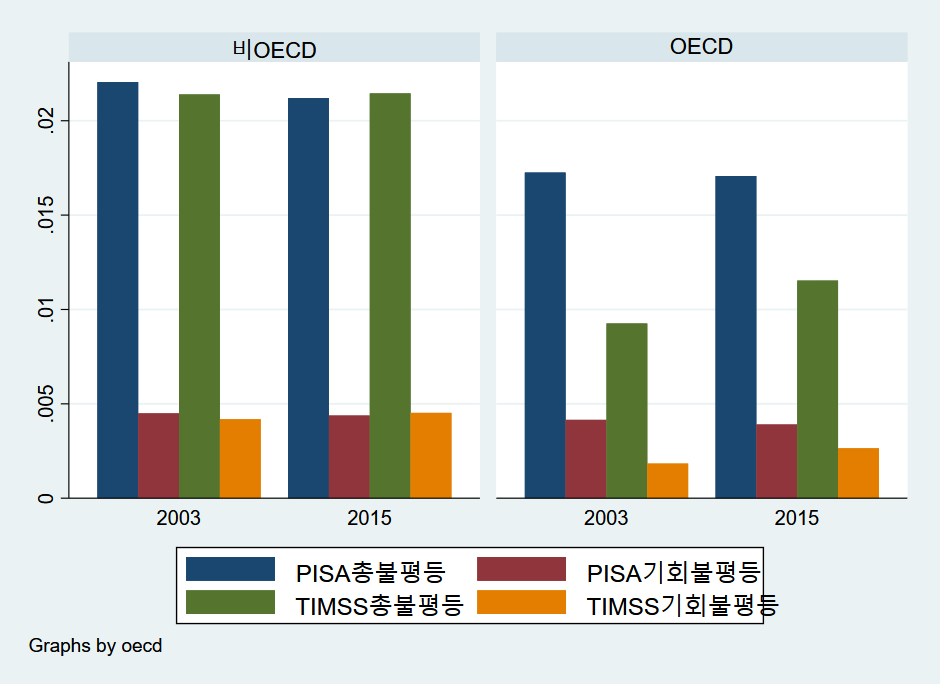
\includegraphics[width=\textwidth]{figure/bar_pntcompare.png}
    \label{fig:bar_pntcompare}
\end{figure}

본 연구에서는 TIMSS의 8학년 학생과 PISA의 학생들에 대한 학업성취도의 총불평등도, 기회불평등도 및 잔여불평등도를 계산한다.
\footnote{정확한 불평등도의 수치와 자료의 기초통계량은 부록에서 제시한다.}
국가별로 학생의 성적을 환경에 대하여 단순선형회귀 하여 환경에 의한 점수와 잔여분에 의한 점수의 추정치를 계산한다. 
여기에 앞서 소개한 \citet{betl12}의 이분산 교정을 이용하여 관측되지 않는 환경에 의한 점수의 추정치를 계산한다.
이 과정에서 환경유형별 오차항의 분산을 추정해야 하기 때문에 특정 유형에 너무 적은 학생이 있을 추정오차가 커지는 문제가 발생한다.
이를 방지하기 위해 환경유형별로 4명 이하의 학생이 존재하는 경우는 분석에서 제외한다.

우리는 두 교육자료에서 제공하는 학생의 수학점수(1st plausible value)를 학생의 학업성취도 성과로서 정의한다.
두 자료는 교육성취를 측정하기 위하여 학생들에게 여러문항의 문제를 제시한다.
각 문항의 점수는 채점이후 문항 반응 이론(item response theory)에 의해 사후적으로 정해지는데 모든 응시생의 평균이 500이고 표준편차가 100으로 조정된 점수가 부여된다.
과목은 수학만을 선정한다. 수학 이외에도 TIMSS는 과학 그리고 PISA는 언어 및 과학 과목의 시험을 더 치른다. 과학과목 역시 두 조사 모두 시행하고 있지만, 과목의 특성상 그 범위가 넓고 실험실의 유무와 같은 국가별 교육환경에 더 영향을 받을 것이다. 이와 같은 영향을 최소화 하기위해 수학과목만을 측정한다. 
 
본 연구에서 환경은 부모의 학력, 가구의 소유물 그리고 가구가 보유한 도서의 수를 이용하여 정의한다.
TIMSS와 PISA 각 자료는 조사시점마다 부친과 모친(또는 남성 및 여성 주 양육자)의 학력을 무학에서 대학원까지 6-7개의 범주형 변수로 제공한다.
우리는 두 개의 학력변수를 단순합 하여 2-12(또는 14)의 항목을 갖는 부모의 학력 변수를 생성한다.
두번째 환경변수는 가구의 소유물 이다.
TIMSS는 매 조사마다 학생의 책상, 방, 인터넷, 컴퓨터 등 네 가지 물건에 대한 소유여부를 조사한다.
PISA의 경우 최대 13가지의 소유물 변수가 존재하지만 자료간 동일성을 유지하기 위해 TIMSS와 유사한 설문 조항 넷을 선택하였다.
모든 소유물 변수는 가변수(Dummy variable) 형태로 값을 취하는데 이를 단순 합하여 0-4의 점수를 가지는 가구 소유물 환경변수를 생성하였다.
마지막으로 장서수는 학생이 속한 가구가 가진 책의 숫자를 10권 미만부터 200권 이상까지 총 1-5의 항목을 가지는 범주형 변수이다.
이상의 세 환경변수에 의한 환경유형은 최대 $13 \times 5 \times 5 = 325$가지 이다.
\footnote{국가에 따라 특정 유형에 한 명도 나오지 않는 경우도 있다.
    예를 들어, 대한민국에서 부모가 모두 대학원졸업 이면서 소유물의 갯수가 0개이고 장서수가 10권 미만인 학생은 없다.} 

\begin{figure}
    \centering
    \caption{1인당GDP와 교육의 총불평등; TIMSS}
    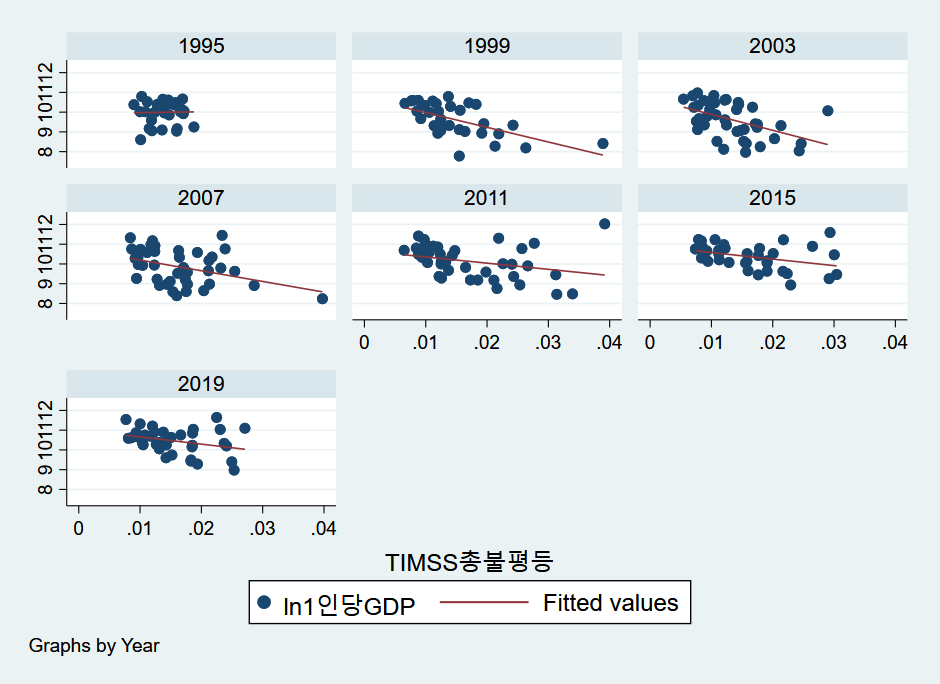
\includegraphics[width=\textwidth]{figure/scatter_lnpcgdp_totmath_timss.png}
    \label{fig:scatter_timss_lnpcgdp_bjtmath}
\end{figure}
그림 (\ref{fig:scatter_timss_lnpcgdp_bjtmath})는 TIMSS 자료상의 국가들의 총불평등과 1인당 국내총생산의 로그값의 관계를 산포도(scatter plot)로 나타낸 것이다.
실선은 각 점들에 대한 맞춤값(fitted value)를 나타냈는데 1995년을 제외한 2000년부터 2019년까지 조사에서 그 값이 모두 우하향 하여 국가의 경제수준과 교육불평등 간에 음의 관계가 있음을 알 수 있다. 

\begin{figure}
    \centering
    \caption{1인당GDP와 교육의 총불평등; OECD vs. 비OECD, TIMSS}
    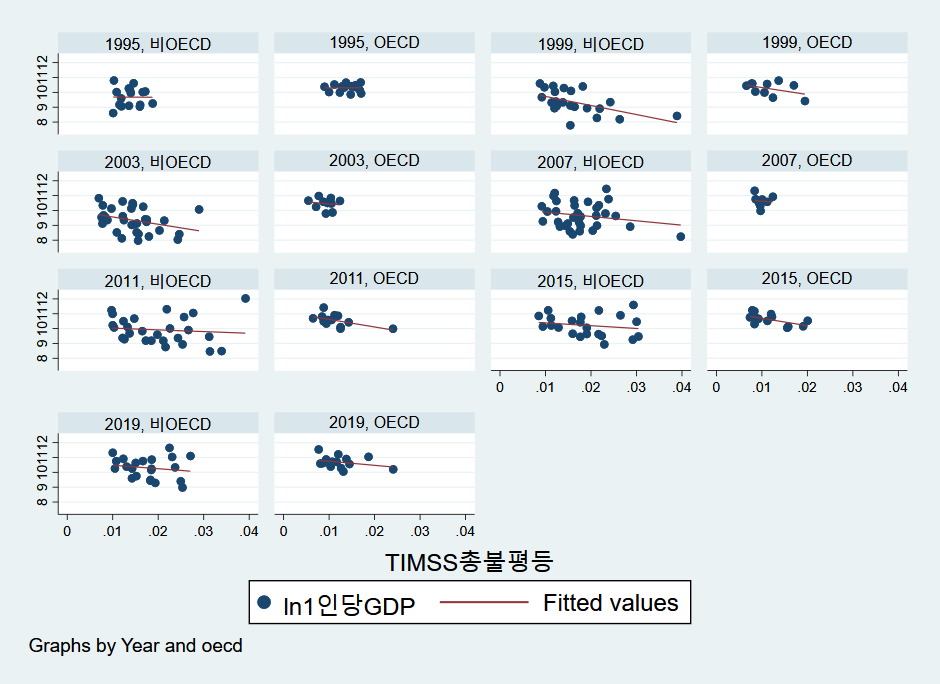
\includegraphics[width=\textwidth]{figure/scatter_lnpcgdp_totmath_timss_oecd.png}
    \label{fig:scatter_timss_lnpcgdp_bjtmath_oecd}
\end{figure}

그림 (\ref{fig:scatter_timss_lnpcgdp_bjtmath_oecd})는 그림 (\ref{fig:scatter_timss_lnpcgdp_bjtmath})을 정보를 OECD 가입국가와 미가입 국가로 나누어 표시하였다.
\footnote{2021년 현재 가입국가는 총 38개국이다. 한국은 1996년 가입하여 TIMSS 1995년을 제외한 나머지 자료에서 OECD 국가로 분류된다. 자세한 가입년도 및 현황은 https://www.oecd.org/about/members-and-partners/ 를 참고하면 된다.}
가장 눈에 띄는 점은 점들의 퍼짐인데, OECD 국가들의 경우 점들이 잘 모여있어 국가별 교육불평등의 정도가 크게 다르지 않음을 알 수 있다. 반면 비OECD 국가의 경우 국가별 1인당 GDP나 교육불형등 수준이 매우 상이함을 알 수 있다.

\begin{figure}
    \centering
    \caption{1인당GDP와 교육의 총불평등; PISA}
    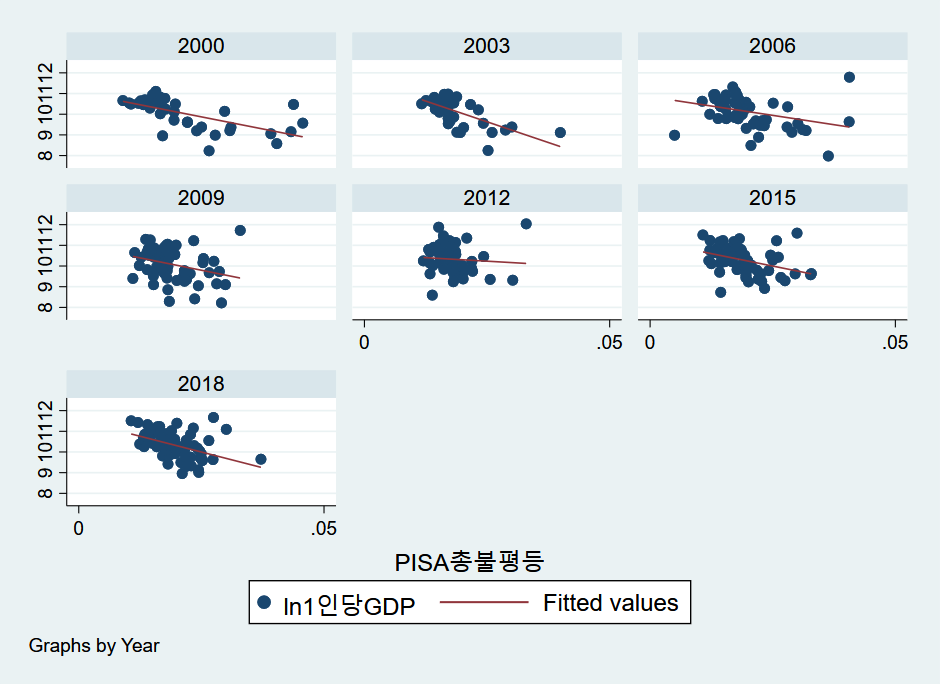
\includegraphics[width=\textwidth]{figure/scatter_lnpcgdp_totmath_pisa.png}
    \label{fig:scatter_pisa_lnpcgdp_bjtmath}
\end{figure}
그림 (\ref{fig:scatter_pisa_lnpcgdp_bjtmath})는 그림 (\ref{fig:scatter_timss_lnpcgdp_bjtmath})와 유사하게 PISA 자료상의 국가들의 총불평등과 1인당 국내총생산의 로그값의 관계를 산포도(scatter plot)로 나타낸 것이다.
2000년부터 2018년까지 조사에서 맞춤값이 모두 우하향 하여 국가의 경제수준과 교육불평등 간에 음의 관계가 있음을 알 수 있다. 

\begin{figure}
    \centering
    \caption{1인당GDP와 교육의 총불평등; OECD vs. 비OECD, PISA}
    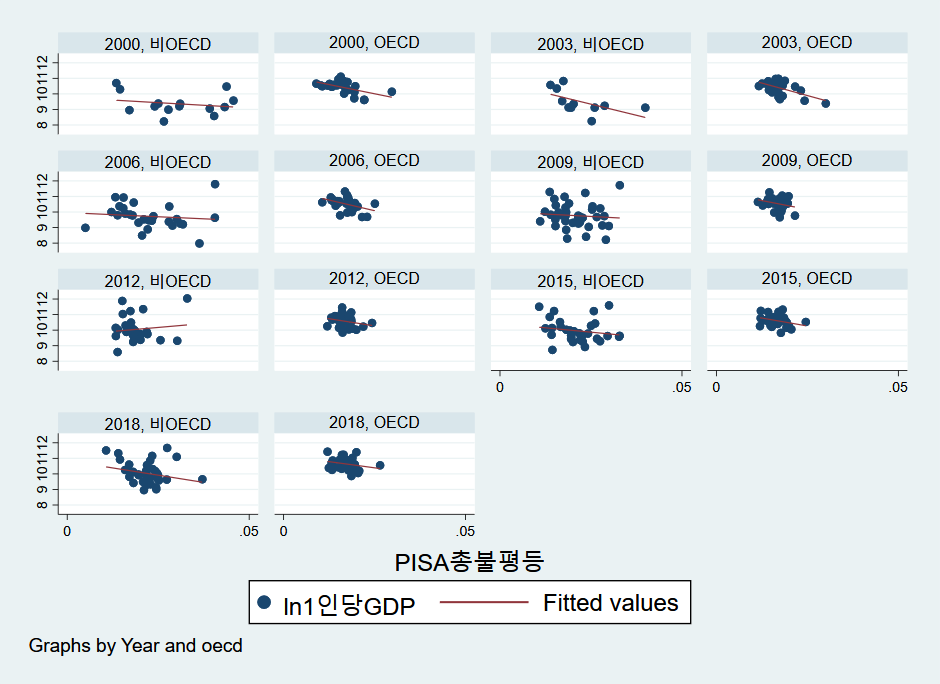
\includegraphics[width=\textwidth]{figure/scatter_lnpcgdp_totmath_pisa_oecd.png}
    \label{fig:scatter_pisa_lnpcgdp_bjtmath_oecd}
\end{figure}

그림 (\ref{fig:scatter_pisa_lnpcgdp_bjtmath_oecd})은 그림 (\ref{fig:scatter_pisa_lnpcgdp_bjtmath})의 내용을 앞서와 마찬가지로 OECD 국가와 비OECD 국가로 나누어 나타낸 것이다.
2012년 비OECD 국가들의 경우 예외적으로 맞춤값이 우상향 하는 것으로 나타나지만 가장 우상단의 극단치인 카타르를 제외한다면 전체적으로 우하향 하는 것으로 볼 수 있다.
 OECD국가들의 점들이 비OECD 국가들에 비해 조밀한 점은 앞서 TIMSS의 경우와 동일하다.
 
\begin{figure}[htpb]
    \centering
    \caption{PISA 총불평등}
    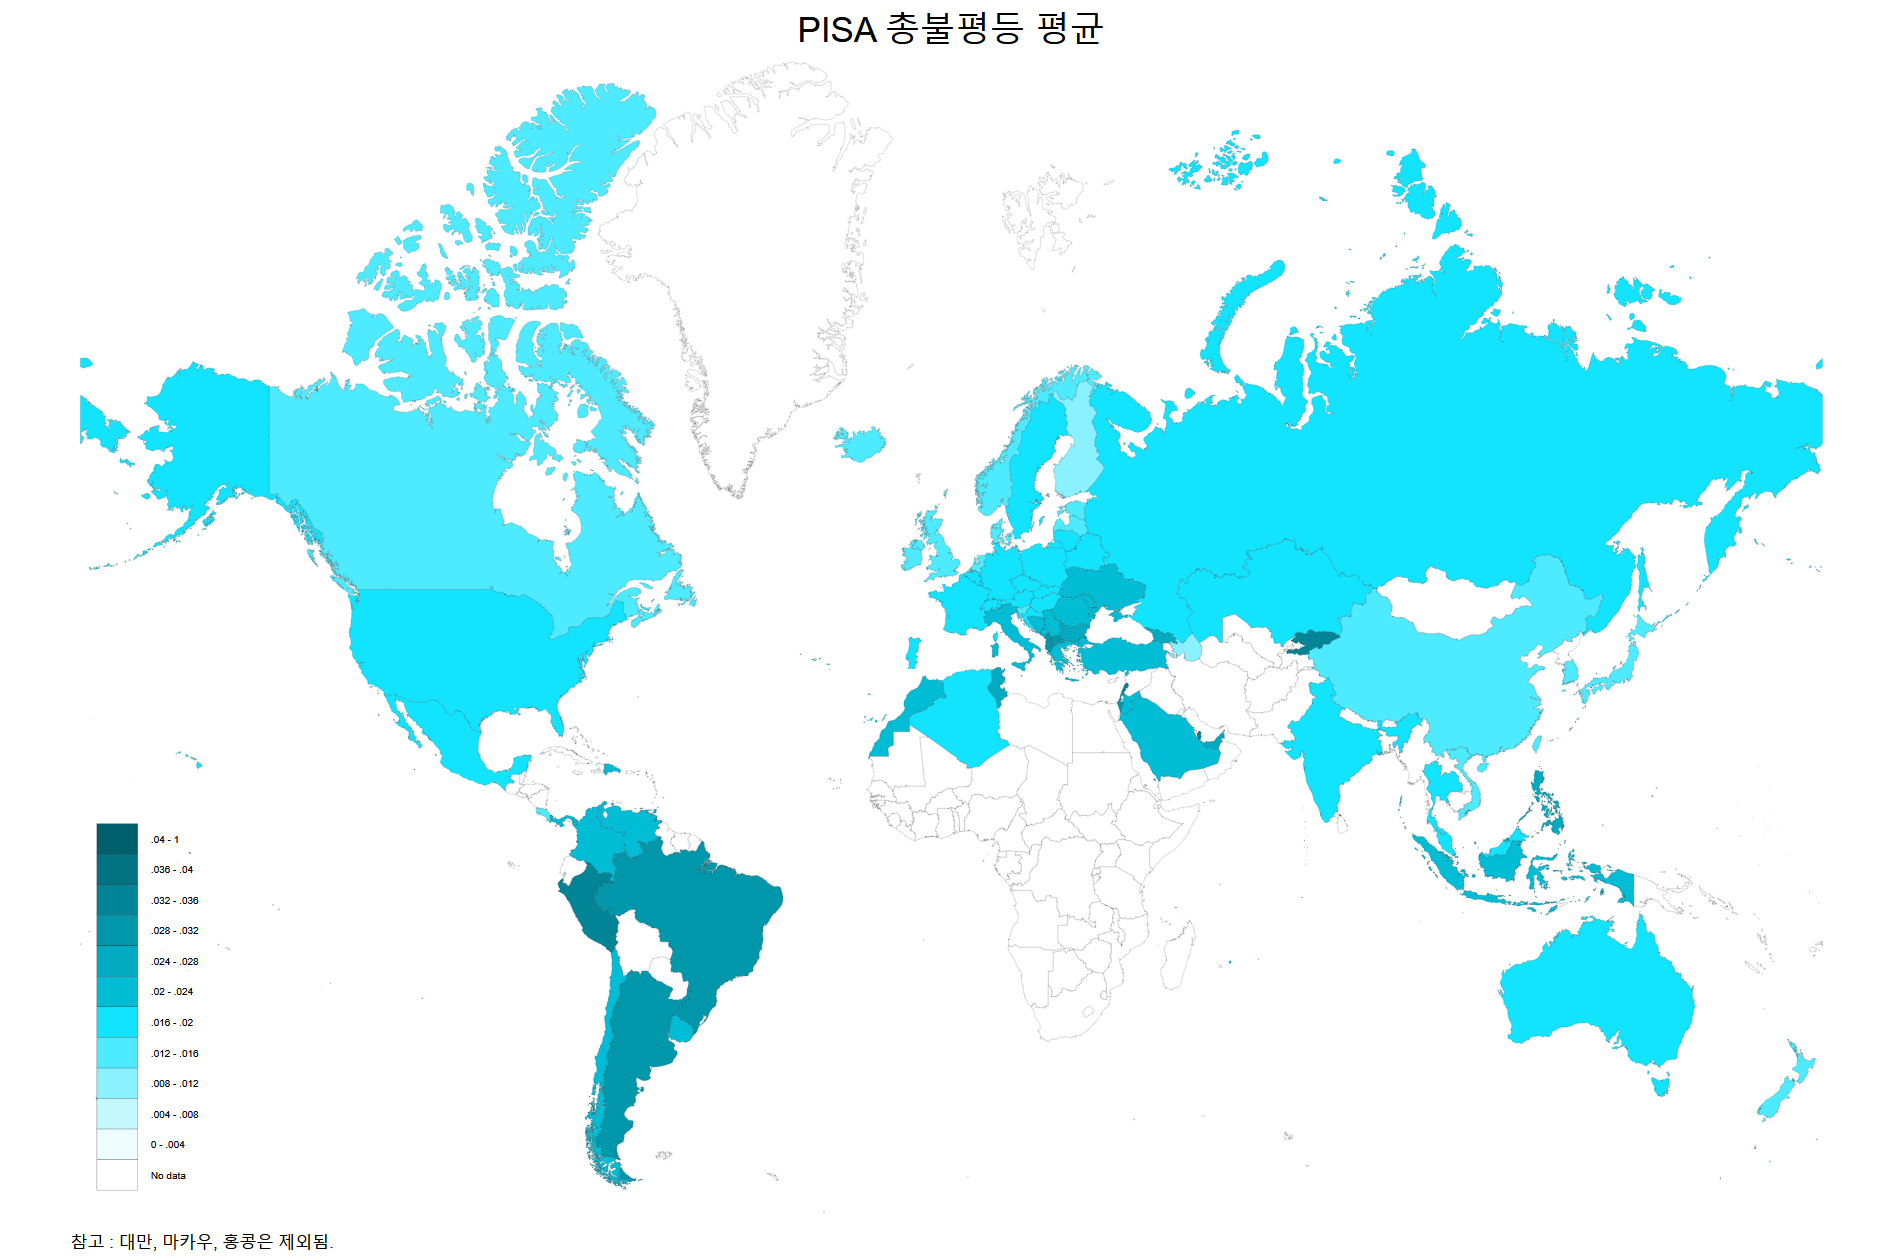
\includegraphics[width=\textwidth]{figure/map_bjtpisa_mean.png}
    \label{fig:map_bjtpisa_mean}
\end{figure}

그림 (\ref{fig:map_bjtpisa_mean})은 PISA 자료를 이용해 측정한 전세계 교육불평등 정도를 2000년 부터 2018년 까지의 평균으로 나타낸 지도이다.
동유럽, 동남아시아, 남아메리카 및 아프리카와 같은 개도국이 많은 지역에서 교육의 총불평등이 높은 것을 확인할 수 있다.
이는 국가의 발전 정도에 맞춰서 발전된 교육제도가 학생들의 교육격차를 줄이는 역할을 하고 있음을 보여준다.

\begin{figure}[htpb]
    \centering
    \caption{PISA 기회불평등의 비중}
    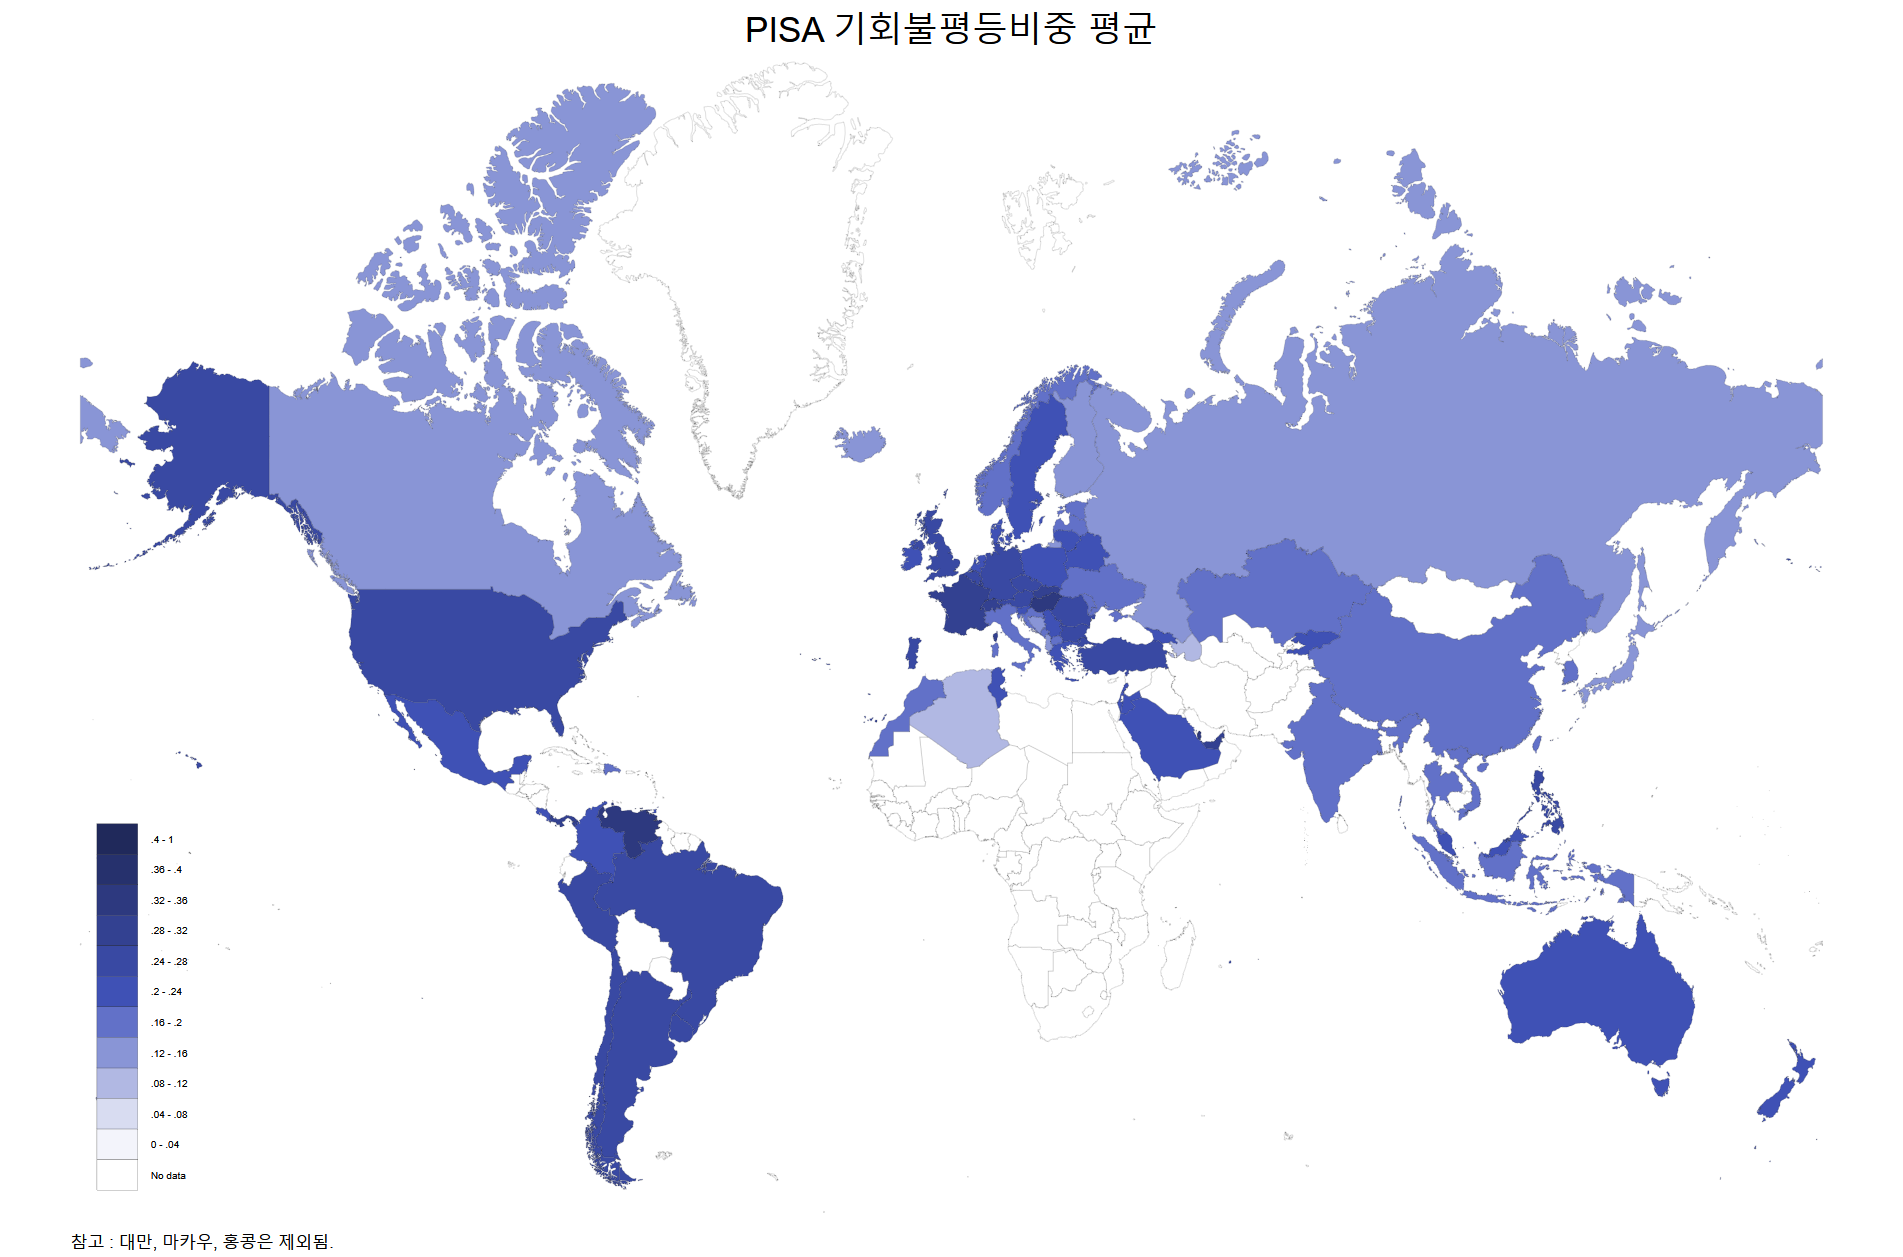
\includegraphics[width=\textwidth]{figure/map_bjrpisa_mean.png}
    \label{fig:map_bjrpisa_mean}
\end{figure}

그림 (\ref{fig:map_bjrpisa_mean})은 그림 (\ref{fig:map_bjtpisa_mean})에서 표시된 총불평등 중에서 기회불평등의 비중이 얼마나 되는가를 나타낸 것이다.
흥미로운 점은 교육의 총불평등이 비교적 낮았던 미국, 서유럽 등의 선진국 지역에서도 기회불평등의 비중은 개도국지역과 비슷하거나 오히려 높은 수준인 것으로 나타났다는 점이다.
선진국의 교육제도가 학생들의 교육격차를 줄이는데 촛점을 맞추고 있다면, 개별 가구에서는 오히려 학생이 좋은 성적을 얻기위한 경쟁에 상당한 영향력을 행사하고 있음을 짐작하게 한다.


그림 (\ref{fig:map_bjrtimss_mean})은 그림 (\ref{fig:map_bjttimss_mean}) 앞선 그림들와 유사하게 TIMSS로 측정한 수학 학업성취도의 총불평등과 총불평등에서 기회불평등의 비중을 1995년 부터 2019년까지 평균값으로 표시한 세계 지도 이다.
TIMSS로 측정한 학업성취도의 경우도 PISA로 측정한 문해도와 마찬가지로 아프리카와 같은 개도국 지역에서 교육의 총불평등도가 높은 반면, 기회불평등의 비중은 서유럽과 같은 선진국에서도 매우 높은 수준임을 확인할 수 있다.

\begin{figure}[htpb]
    \centering
    \caption{TIMSS 총불평등}
    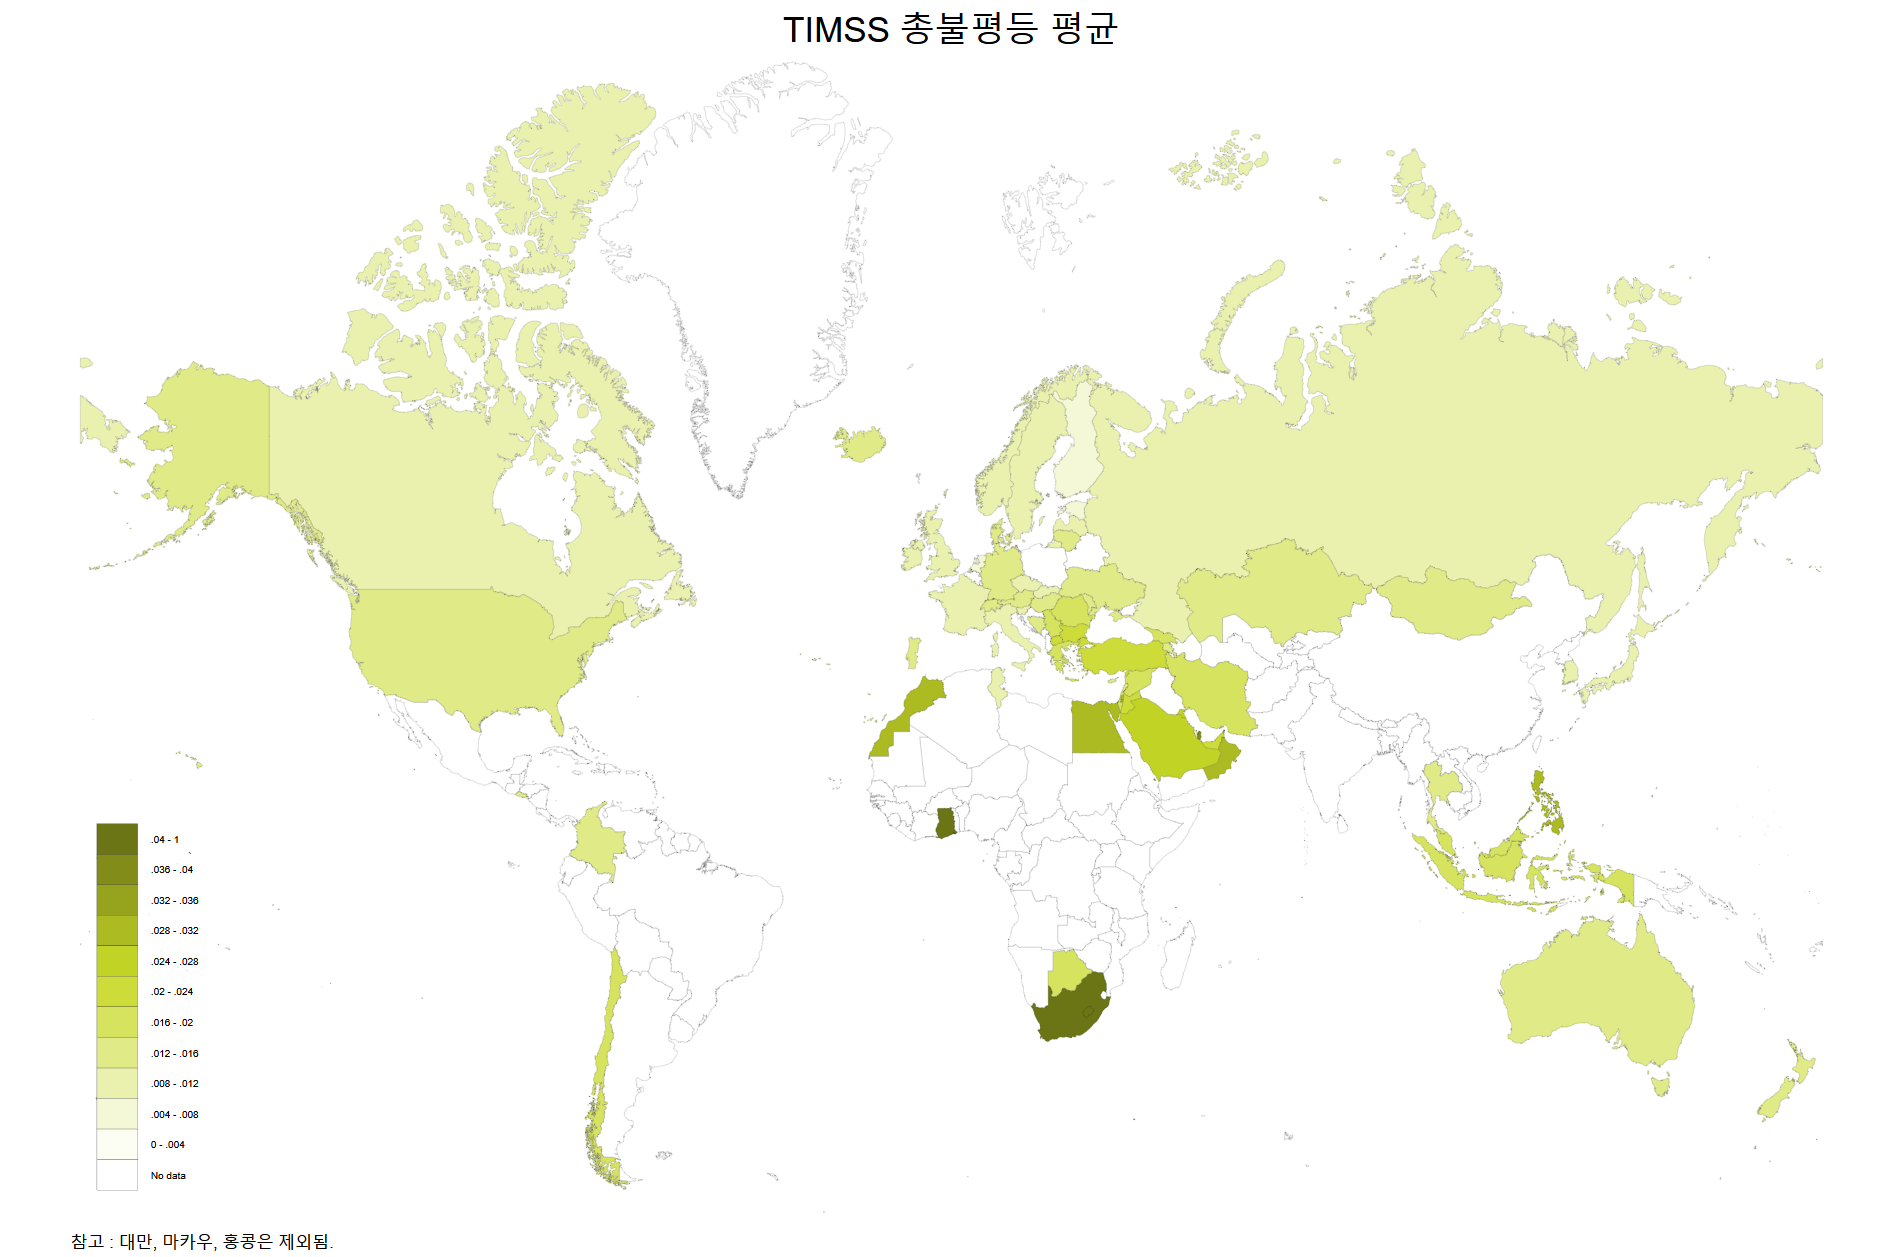
\includegraphics[width=\textwidth]{figure/map_bjttimss_mean.png}
    \label{fig:map_bjttimss_mean}
\end{figure}

\begin{figure}[htpb]
    \centering
    \caption{TIMSS 기회불평등의 비중}
    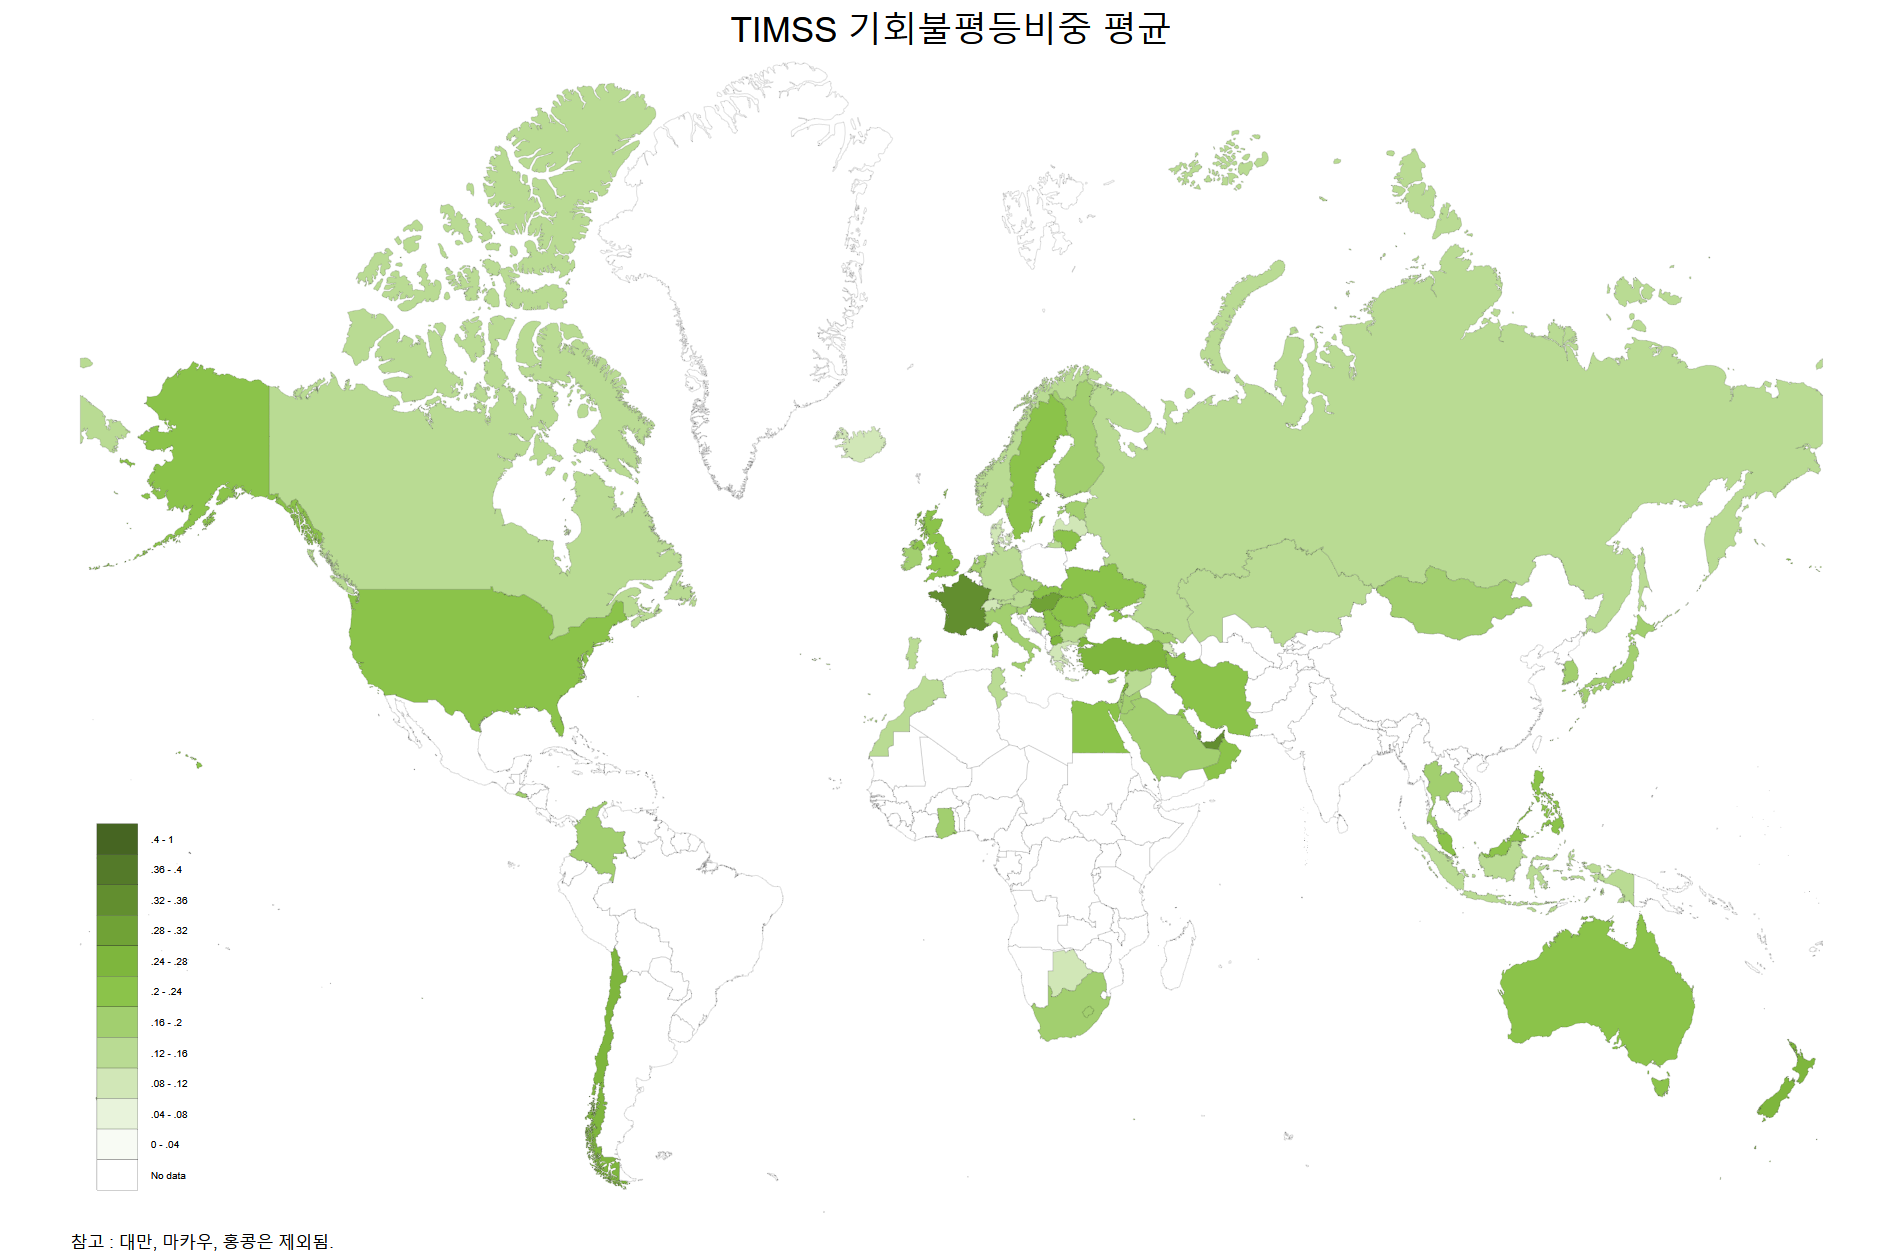
\includegraphics[width=\textwidth]{figure/map_bjrtimss_mean.png}
    \label{fig:map_bjrtimss_mean}
\end{figure}
    
\subsection{실증분석 모형}

본 연구에서 우리는 성장 회귀분석(growth regression)에서 일반적으로 사용하는 다음의 실증모형을 추정한다.
\begin{equation}
 \begin{aligned}
 \ln \left(Y_{i, t^{\prime}}\right)-\ln \left(Y_{i, t}\right)=& \delta_{1} I O P_{i, t}+\delta_{2} I O E_{i, t}+\beta_{1} \ln \left(Y_{i, t}\right)+X_{i, t} \beta_{2} \\
 &+\alpha_{i}+\tau_{t^{\prime}}+u_{i, t^{\prime}}
 \end{aligned}
 \label{eq:regbase}
\end{equation} 
 위 식에서 $i$는 국가를, $t$는 교육기회불평등의 측정연도이다. $t'$는 다음 조사시점을 의미하는데 개별 회귀분석마다 다를 수 있다. 연구의 편의를 위해 각 자료의 조사 주기를 따르기로 한다. 따라서 TIMSS의 경우 $t'=t+4$ 이고 PISA의 경우  $t'=t+3$이다. $Y_{i,t}$는 국가 $i$의 연도 $t$현재 1인당 GDP, $Y_{i,t'}$는 국가 $i$의 년도 $t'$현재 1인당 GDP를 표시한다. $\ln \left(Y_{i, t^{\prime}}\right)-\ln \left(Y_{i, t}\right)$ 는 국가 $i$의 연도 $t$에서 연도 $t'$까지 1인당 GDP의 성장률을 표시한다. 
 
우리는 먼저 식 (\ref{eq:regbase})의 종속변수로서 한 국가의 다음 조사기간의 경제성장률을 사용한다. 
$IOP_{i,t}$는 국가 $i$의 $t$연도 현재 교육 기회불평등 지수의 값이고, $IOE_{i,t}$ 는 총불평등에서 기회의 불평등에 의해 설명되지 않는 잔여불평등(노력 불평등의 대리 지표)을 표시한다. $X_{i,t}$는 국가 $i$의 $t$연도 현재 특성변수들로 인구의 로그값과 경제의 대외개방도를 가늠할 수 있는 투자재의 가격의 벡터이다. $\alpha _i$는 국가 고정효과, 그리고 $\tau _{t'}$는 연도 고정효과를 표시한다.

실제 회귀분석은 식 (\ref{eq:regbase})을 일부 수정한 식 (\ref{eq:regmod})에 대해 선형회귀분석(OLS), 패널 고정효과(fixed effect) 모형, 시스템 GMM(\citet{bnb98}) 방법을 적용함으로써 주요 계수들을 추정한다.

\begin{equation}
 \begin{aligned}
 \ln \left(Y_{i, t^{\prime}}\right)=& \delta_{1} I O P_{i, t}+\delta_{2} I O E_{i, t}+\left(\beta_{1}+1\right) \ln \left(Y_{i, t}\right)+X_{i, t} \beta_{2} \\
 &+\alpha_{i}+\tau_{t^{\prime}}+u_{i, t^{\prime}}
 \end{aligned}
 \label{eq:regmod}
\end{equation}

\section{분석 결과}
\subsection{그림을 통한 분석}

\begin{figure}
    \centering
    \caption{1인당GDP성장률과 교육의 총불평등; TIMSS}
    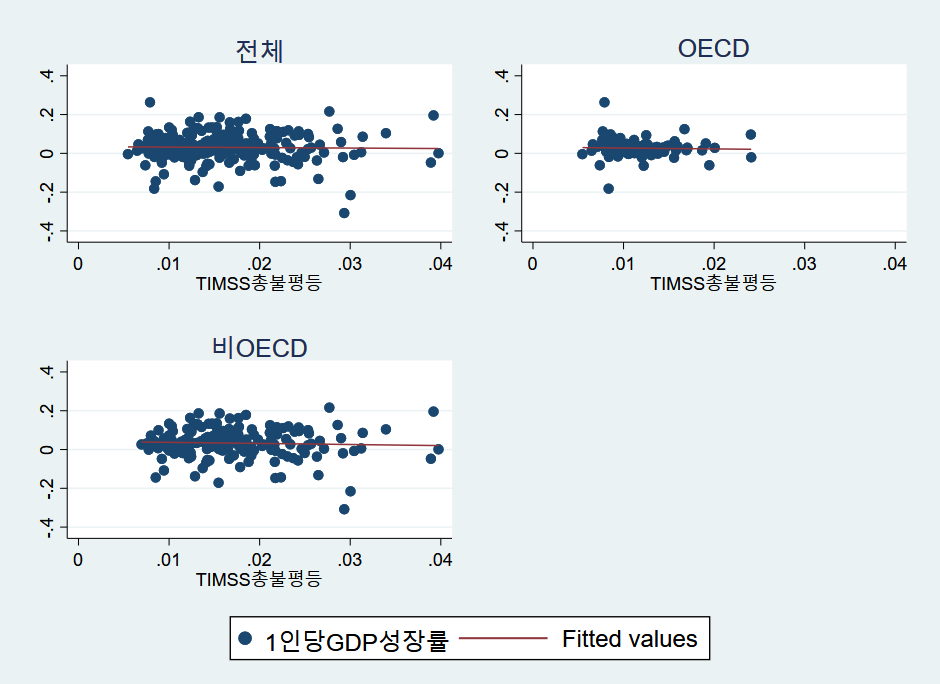
\includegraphics[width=\textwidth]{figure/scatter_pcgrowth_totmath_timss_noy.png}
    \label{fig:scatter_timss_pcgrowth_bjtmath_noy}
\end{figure}


\begin{figure}
    \centering
    \caption{1인당GDP성장률과 교육의 총불평등; PISA}
    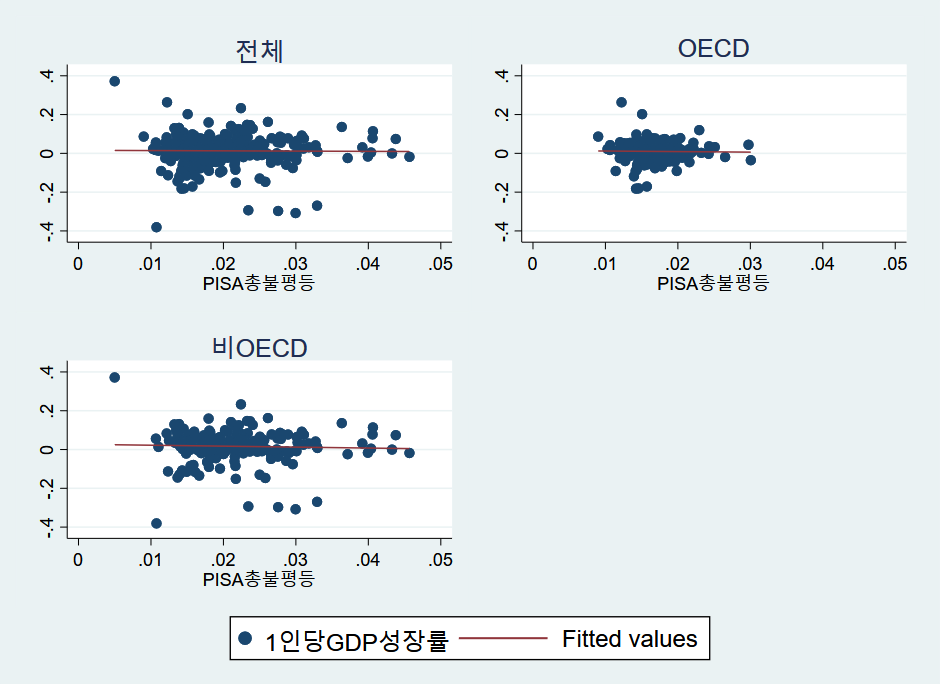
\includegraphics[width=\textwidth]{figure/scatter_pcgrowth_totmath_pisa_noy.png}
    \label{fig:scatter_pisa_pcgrowth_bjtmath_noy}
\end{figure}

그림 (\ref{fig:scatter_timss_pcgrowth_bjtmath_noy})과 (\ref{fig:scatter_pisa_pcgrowth_bjtmath_noy})의 Y축 변수로서 우리는 아래의 식 (\ref{eq:lfit})에 OLS를 적용해 구한 잔차(즉 $\ln \left(Y_{i, t'}\right)-\left[\widehat{\tau_{0}}+\widehat{\tau_{1}} \ln \left(Y_{i, t}\right)\right]$ )를 사용한다. 
한편 X축에 표시되어 있는 변수는 각국의 총불평등도 지수들이다.
\begin{equation}
\label{eq:lfit}
\ln \left(Y_{i, t'}\right)=\tau_{0}+\tau_{1} \ln \left(Y_{i, t}\right)+\epsilon_{i, t'}
\end{equation}
(\ref{fig:scatter_timss_pcgrowth_bjtmath_noy})에 (\ref{fig:scatter_pisa_pcgrowth_bjtmath_noy})에 의하면, 성적의 총불평등도는 대체로 경제성장에 부정적인 영향을 미치지만 그 효과는 다소 상이해 보인다.
이러한 부정적 영향은 OECD 국가들과 비OECD 국가들에서 동시에 관찰 된다.

\subsection{회귀 분석 결과}
본 절에서 우리는 본 연구의 자료를 사용해 불평등도와 경제성장 사이의 관계를 분석한 선행 실증연구들을 재현해 본다. 이를 통해 본 연구에서 사용하는 주요 자료들이 선행 연구에서 사용했던 자료와 비슷한 경향성을 보이는지를 확인할 수 있다.  표 (\ref{tab:pisa_reg1})에는 아래의 식 (\ref{eq:simplereg})를 추정한 결과가 제시되어 있다. 식 (\ref{eq:simplereg})는 불평등과 경제성장 사이의 관계를 다룬 많은 성장 회귀분석 연구에서 가장 빈번하게 사용되는 추정모형이다.
\begin{equation}
\label{eq:simplereg}
\ln \left(Y_{i, t'}\right)=\delta \operatorname{Ineq}_{i, t}+\left(\beta_{1}+1\right) \ln \left(Y_{i, t}\right)+X_{i, t} \beta_{2}+\alpha_{i}+\tau_{t'}+u_{i, t'}
\end{equation}
위 식에서 $Ineq_{i,t}$는 국가 $i$의 연도 $t$ 현재 성적의 총불평등도 지수이다. 식 (\ref{eq:simplereg})를 추정함으로써 우리는 TIMSS의 성적 불평등 지수를 사용하는 경우에도 전통적인 성장 회귀분석의 추정결과가 유사하게 나타나는지를 확인하고자 한다. 본 연구의 핵심 실증모형인 식 (\ref{eq:regmod})은 식 (\ref{eq:simplereg})의 $\delta Ineq_{i,t}$를 $\delta_{1} I O P_{i, t}+\delta_{2} I O E_{i, t}$와 같이 분해한 모형으로서 해석할 수 있다.
 
표 (\ref{tab:timss_reg1})의 (1)-(3)열은 전체 표본에 대해 각각 OLS, 패널 고정효과(Fixed Effects, FE), 시스템 GMM(Generalized Method of Moments) 추정법을 적용해 구한 추정치를 제시하고 있다.
OLS 추정법은 국가들 사이의 보이지 않는 이질성을 적절히 통제하지 못한다.
 이러한 국가 간 이질성의 문제를 통제하기 위해 패널 고정효과 모형을 사용하는 경우에도, $ln(Y_{i,t})$의 내생성 때문에 핵심 계수의 일치추정량을 구하기 어렵다고 알려져 있다.
위의 두 문제를 동시에 해결하기 위해 최근의 성장 회귀분석에서는 동태적 패널분석법(dynamic panel data analysis)의 하나인 시스템 GMM 추정법(\citet{bnb98})을 적용한다.
이하에서는 시스템 GMM 추정치들을 중심으로 분석결과를 설명하고자 한다.

%아울러 성적의 총불평등이 경제성장에 미치는 효과가 국가의 특성에 따라 서로 상이한지를 검증하기 위해 우리는 식 (\ref{eq:regmod})의 불평등부분을 $\delta$ Ineq $_{i, t}=\delta_{N} N O E C D_{i} \times$ Ineq $_{i, t}+\delta_{O} O E C D_{i} \times$ Ineq $_{i, t}$ 와 같이 분해한다.
%여기에서 $OECD_i$ 는 국가 $i$가 $t$년도 현재 OECD 가입국이면 1, 그렇지 않으면 0을 취하는 더미변수이고, $NOECD_i$는 반대로 비OECD 국가에 대한 더미변수 이다.
%표 (\ref{tab:timss_reg1})의 (4)-(6)열에는 전체 표본을 비 OECD 국가 집단과 OECD 국가 집단으로 구분한 경우의 추정치가 제시되어 있다.  

\label{ans6}
아울러 교육의 총불평등이 경제성장에 미치는 효과가 국가의 특성에 따라 서로 상이한지를 검증하기 위해 우리는 식 (\ref{eq:simplereg})에 OECD 가입여부에 대한 가변수를 이용한 변형을 한다.
불평등지수의 항인 $\delta$ Ineq $_{i, t}$를 $\delta_{1} Ineq _{i, t}  + \delta _{2} O E C D_{i} \times$ Ineq $_{i, t} + \delta_{3} O E C D_{i} $로 대체한다.
여기에서 $OECD_i$ 는 국가 $i$가 $t$년도 현재 OECD 가입국이면 1, 그렇지 않으면 0을 취하는 가변수이다.
따라서 $\delta _ 1$은 개별 국가의 특성에 상관없이 불평등이 경제성장에 미치는 영향을 나타낸다. 
$\delta _ 2$는 비교적 발전이 진행된 OECD 가입국에서 불평등정도가 경제성장에 미치는 영향을 각각 나타낸다.
$\delta _ 3$는 OECD로 가입여부로 나타낸 국가의 발전정도가 경제성장에 미치는 영향을 나타낸다.
표 (\ref{tab:timss_reg1})의 (4)-(6)열에는 전체 표본을 비 OECD 국가 집단과 OECD 국가 집단으로 구분한 경우의 추정치가 제시되어 있다.  

\begin{table}[htbp]\centering
\def\sym#1{\ifmmode^{#1}\else\(^{#1}\)\fi}
\caption{회귀분석 결과 : TIMSS, 총불평등 \label{tab:timss_reg1}}
\resizebox{\textwidth}{!}{
\begin{tabular}{l*{6}{c}}
\hline\hline
                    &\multicolumn{1}{c}{(1)}&\multicolumn{1}{c}{(2)}&\multicolumn{1}{c}{(3)}&\multicolumn{1}{c}{(4)}&\multicolumn{1}{c}{(5)}&\multicolumn{1}{c}{(6)}\\
                    &\multicolumn{1}{c}{OLS}&\multicolumn{1}{c}{FE}&\multicolumn{1}{c}{Sys. GMM}&\multicolumn{1}{c}{OLS}&\multicolumn{1}{c}{FE}&\multicolumn{1}{c}{Sys. GMM}\\
\hline
총불평등          &      -1.172\sym{*}  &       0.199         &      -4.649\sym{*}  &      -1.220\sym{*}  &      0.0398         &      -3.828\sym{*}  \\
                    &     (0.666)         &     (0.803)         &     (2.427)         &     (0.707)         &     (0.802)         &     (2.256)         \\
[1em]
OECD $\times$ 총불평등&                     &                     &                     &       6.624         &       13.40\sym{**} &       13.31\sym{*}  \\
                    &                     &                     &                     &     (4.072)         &     (6.678)         &     (7.506)         \\
[1em]
OECD              &                     &                     &                     &     -0.0595         &      -0.151         &    -0.00967         \\
                    &                     &                     &                     &    (0.0526)         &    (0.0997)         &     (0.118)         \\
[1em]
ln1인당GDP        &       0.927\sym{***}&       0.570\sym{***}&       0.807\sym{***}&       0.925\sym{***}&       0.570\sym{***}&       0.775\sym{***}\\
                    &    (0.0146)         &    (0.0550)         &    (0.0652)         &    (0.0148)         &    (0.0549)         &    (0.0731)         \\
[1em]
투자재가격        &      0.0640         &      -0.148         &      0.0628         &      0.0599         &      -0.138         &    -0.00241         \\
                    &    (0.0491)         &    (0.0901)         &     (0.105)         &    (0.0551)         &    (0.0898)         &    (0.0921)         \\
[1em]
ln인구            &    -0.00920         &      -0.320\sym{***}&      -0.174\sym{**} &     -0.0112\sym{*}  &      -0.327\sym{***}&      -0.222\sym{***}\\
                    &   (0.00606)         &    (0.0988)         &    (0.0714)         &   (0.00670)         &    (0.0985)         &    (0.0811)         \\
[1em]
Constant            &       0.842\sym{***}&       5.384\sym{***}&       2.518\sym{***}&       0.864\sym{***}&       5.402\sym{***}&       2.918\sym{***}\\
                    &     (0.135)         &     (0.641)         &     (0.670)         &     (0.139)         &     (0.644)         &     (0.726)         \\
\hline
r2                  &       0.974         &       0.820         &                     &       0.975         &       0.824         &                     \\
관측수                   &         238         &         238         &         238         &         238         &         238         &         238         \\
국가수                 &                     &          71         &          71         &                     &          71         &          71         \\
\hline\hline
\multicolumn{7}{l}{\footnotesize 괄호안은 표준오차.}\\
\multicolumn{7}{l}{\footnotesize \sym{*} \(p<0.10\), \sym{**} \(p<0.05\), \sym{***} \(p<0.01\)}\\
\end{tabular}}
\end{table}


먼저 TIMSS의 경우를 살펴본다.
회귀분석에는 총 71개국에서 238개 불평등 지수가 측정되어 한 국가당 약 3회 정도의 관측치가 사용되었다.
ln1인당GDP의 계수는 식 (\ref{eq:simplereg})에 의하면 1이 더해진 값임에 주의해야 한다. 따라서 표에 제시된 계수들에서 1을 차감한 값이 추정된 값으로 1인당 GDP가 이미 높은 수준일수록 경제성장률이 낮다는 상식에 부합한다.
표 (\ref{tab:timss_reg1})의 (3)열을 보면, 학업성취도의 총불평등도는 4년 후의 1인당 GDP에 유의미한 부정적 관계(추정치 -4.649)를 가진다.
OECD 가입여부를 구분해서 살펴보는 (6)열에 의하면, 학업성취도의 불평등은 -3.828로 유의미한 음의 관계를 보이는 반면 OECD국가들에서는 13.31로 유의미한 양의 상관관계를 나타냈다. 
OECD 국가라는 사실은 유의미한 영향을 주지 못하는 것으로 보였다.
이는 국가별 발전정도에 따라 불평등이 경제성장에 미치는 영향이 정 반대로 나타날 수 있음을 보여주고 있다.
이 추정치를 한국의 경우를 예로 들어 해석하면 다음과 같다.
2003년 한국의 총불평등은 0.0071인데 2007년은 0.0095로 0.0024 증가 하였다.
 증가분에 추정된 계수값 13.31을 곱한 수치는 약 0.032로 수학 학업성취도의 총불평등 증가는 한국의 4년간 경제성장률을 약 3.2\%포인트 상승시켰을 것으로 추정된다.
 실제 한국의 2007년에서 2011년 사이 경제성장률은 약 2.3\% 이었으므로, 2007년도의 한국의 학업성취도 불평등도가 2003년 수준으로 유지되었다면, 2007년과 2011년 사이의 경제성장률은 -0.9\%이었을 것으로 추정된다.

\begin{table}[htbp]\centering
\def\sym#1{\ifmmode^{#1}\else\(^{#1}\)\fi}
\caption{회귀분석 결과 : TIMSS, 기회 vs. 잔여불평등 \label{tab:timss_reg2}}
\resizebox{\textwidth}{!}{
\begin{tabular}{l*{6}{c}}
\hline\hline
                    &\multicolumn{1}{c}{(1)}&\multicolumn{1}{c}{(2)}&\multicolumn{1}{c}{(3)}&\multicolumn{1}{c}{(4)}&\multicolumn{1}{c}{(5)}&\multicolumn{1}{c}{(6)}\\
                    &\multicolumn{1}{c}{OLS}&\multicolumn{1}{c}{FE}&\multicolumn{1}{c}{Sys. GMM}&\multicolumn{1}{c}{OLS}&\multicolumn{1}{c}{FE}&\multicolumn{1}{c}{Sys. GMM}\\
\hline
기회불평등        &      -1.750         &      -1.374         &      -16.65\sym{**} &      -1.553         &      -2.401         &      -15.11\sym{*}  \\
                    &     (5.203)         &     (5.169)         &     (7.331)         &     (5.534)         &     (5.291)         &     (7.734)         \\
[1em]
잔여불평등        &      -1.053         &       0.483         &      -2.334         &      -1.184         &       0.475         &      -1.620         \\
                    &     (1.204)         &     (1.222)         &     (2.566)         &     (1.292)         &     (1.231)         &     (2.339)         \\
[1em]
OECD $\times$ 기회불평등&                     &                     &                     &      -6.446         &       13.03         &      -2.922         \\
                    &                     &                     &                     &     (12.79)         &     (20.68)         &     (19.52)         \\
[1em]
OECD $\times$ 잔여불평등&                     &                     &                     &       10.34         &       13.88\sym{*}  &       19.41\sym{**} \\
                    &                     &                     &                     &     (6.320)         &     (8.089)         &     (7.735)         \\
[1em]
OECD              &                     &                     &                     &     -0.0637         &      -0.156         &     -0.0299         \\
                    &                     &                     &                     &    (0.0553)         &     (0.101)         &     (0.114)         \\
[1em]
ln1인당GDP        &       0.928\sym{***}&       0.568\sym{***}&       0.817\sym{***}&       0.925\sym{***}&       0.567\sym{***}&       0.780\sym{***}\\
                    &    (0.0145)         &    (0.0553)         &    (0.0671)         &    (0.0149)         &    (0.0554)         &    (0.0764)         \\
[1em]
투자재가격        &      0.0630         &      -0.149         &      0.0520         &      0.0587         &      -0.138         &     0.00736         \\
                    &    (0.0480)         &    (0.0904)         &    (0.0948)         &    (0.0540)         &    (0.0915)         &    (0.0841)         \\
[1em]
ln인구            &    -0.00923         &      -0.318\sym{***}&      -0.178\sym{**} &     -0.0111\sym{*}  &      -0.325\sym{***}&      -0.224\sym{***}\\
                    &   (0.00608)         &    (0.0993)         &    (0.0731)         &   (0.00668)         &    (0.0993)         &    (0.0824)         \\
[1em]
Constant            &       0.839\sym{***}&       5.393\sym{***}&       2.446\sym{***}&       0.869\sym{***}&       5.419\sym{***}&       2.869\sym{***}\\
                    &     (0.134)         &     (0.644)         &     (0.684)         &     (0.140)         &     (0.648)         &     (0.750)         \\
\hline
r2                  &       0.974         &       0.820         &                     &       0.975         &       0.825         &                     \\
관측수                   &         238         &         238         &         238         &         238         &         238         &         238         \\
국가수                 &                     &          71         &          71         &                     &          71         &          71         \\
\hline\hline
\multicolumn{7}{l}{\footnotesize 괄호안은 표준오차.}\\
\multicolumn{7}{l}{\footnotesize \sym{*} \(p<0.10\), \sym{**} \(p<0.05\), \sym{***} \(p<0.01\)}\\
\end{tabular}}
\end{table}

표 \ref{tab:timss_reg2}는 표 \ref{tab:timss_reg1}의 총불평등을 기회불평등과 잔여불평등으로 분해하여 회귀분석한 결과이다.
(3)열을 보면, 학업성취도의 기회불평등도의 계수는 -16.65로 4년 후의 1인당 GDP에 유의미한 부정적 관계를 가진다.
OECD 가입여부를 구분해서 살펴보는 (6)열에 의하면, 기회불평등의 계수값은 -15.11로 기회불평등이 커질수록 경제성장에 부정적 영향을 주는 것을 확인했다.
OECD 국가들의 경우로 제한해서 살펴보면 학업성취도의 기회불평등은 OECD국가들에서 유의미한 영향을 주지 못하였다. 
반면 잔여불평등은 계수값이 19.41으로 유의미한 긍정적 영향을 주는 것을 확인하였다.
다시 말해, 앞서 학업성취도의 불평등이 커질수록 경제성장에 긍정적 영향을 준다는 결과는 환경에서 비롯되지 않은 개인의 순수한 노력을 포함한 요소에 의한 성적 격차의 증가가 경제성장에 긍정적 영향을 준다는 의미이다.

\centering
\def\sym#1{\ifmmode^{#1}\else\(^{#1}\)\fi}
\caption{PISA 총불평등\label{tab:pisasimp}}
\begin{tabular}{l*{6}{c}}
\toprule
                    &\multicolumn{1}{c}{(1)}&\multicolumn{1}{c}{(2)}&\multicolumn{1}{c}{(3)}&\multicolumn{1}{c}{(4)}&\multicolumn{1}{c}{(5)}&\multicolumn{1}{c}{(6)}\\ &\multicolumn{1}{c}{OLS}&\multicolumn{1}{c}{FE}&\multicolumn{1}{c}{Sys. GMM}&\multicolumn{1}{c}{OLS}&\multicolumn{1}{c}{FE}&\multicolumn{1}{c}{Sys. GMM}\\
\midrule
총불평등          &      -3.248\sym{***}&      -4.625\sym{***}&      -2.332         &                     &                     &                     \\
                    &     [-2.99]         &     [-3.27]         &     [-0.58]         &                     &                     &                     \\
\addlinespace
OECD$ \times$ 총불평등&                     &                     &                     &      -3.562\sym{***}&      -2.107         &       0.737         \\
                    &                     &                     &                     &     [-2.70]         &     [-0.95]         &      [0.12]         \\
\addlinespace
비OECD$ \times$ 총불평등&                     &                     &                     &      -3.268\sym{***}&      -4.875\sym{***}&      -3.968         \\
                    &                     &                     &                     &     [-3.00]         &     [-3.43]         &     [-1.08]         \\
\midrule
r2                  &       0.980         &       0.803         &                     &       0.980         &       0.804         &                     \\
N                   &         334         &         334         &         334         &         334         &         334         &         334         \\
N\_g                 &                     &          77         &          77         &                     &          77         &          77         \\
\bottomrule
\multicolumn{7}{l}{\footnotesize \textit{t} statistics in brackets}\\
\multicolumn{7}{l}{\footnotesize \sym{*} \(p<0.10\), \sym{**} \(p<0.05\), \sym{***} \(p<0.01\)}\\
\end{tabular}


지금부터는 PISA 자료를 이용하여 문해력의 불평등이 경제성장에 미치는 영향을 살펴본다.
PISA 자료에는 77개 국에서 총 358회의 불평등지수를 측정하였으며 이는 국가별로 평균 4회에 해당한다.
PISA로 측정한 문해력의 불평등과 경제성장간의 관계는 앞서 살펴본 학업성취도의 불평등과는 다른 모습을 보인다.
표 (\ref{tab:pisa_reg1})에 제시된 분석 결과를 요약하면 다음과 같다.
OLS와 FE 추정방법을 사용하는 경우에도 유의미했던 부정적 관계가 시스템 GMM 추정법을 사용할 경우 유의성이 없는 것으로 나타났다.
이는 TIMSS의 경우 유의미한 부정적 관계를 보인것과 상이하다.
(6)열에 의하면, 문해력의 불평등은 (3)열의 경우와 마찬가지로 OECD 가입 여부를 나누어 고려하더라도 유의미한 영향을 주지 못하는 것으로 나타났다.

\begin{table}[htbp]\centering
\def\sym#1{\ifmmode^{#1}\else\(^{#1}\)\fi}
\caption{회귀분석 결과 : PISA, 기회 vs. 잔여불평등 \label{tab:pisa_reg2}}
\resizebox{\textwidth}{!}{
\begin{tabular}{l*{6}{c}}
\hline\hline
                    &\multicolumn{1}{c}{(1)}&\multicolumn{1}{c}{(2)}&\multicolumn{1}{c}{(3)}&\multicolumn{1}{c}{(4)}&\multicolumn{1}{c}{(5)}&\multicolumn{1}{c}{(6)}\\
                    &\multicolumn{1}{c}{OLS}&\multicolumn{1}{c}{FE}&\multicolumn{1}{c}{Sys. GMM}&\multicolumn{1}{c}{OLS}&\multicolumn{1}{c}{FE}&\multicolumn{1}{c}{Sys. GMM}\\
\hline
기회불평등        &      -2.924         &      -0.375         &       9.860         &      -6.456         &       1.176         &       4.884         \\
                    &     (4.964)         &     (6.002)         &     (11.29)         &     (7.345)         &     (7.213)         &     (12.28)         \\
[1em]
잔여불평등        &      -3.371\sym{**} &      -5.716\sym{***}&      -6.400\sym{*}  &      -2.601         &      -6.889\sym{***}&      -6.563         \\
                    &     (1.680)         &     (2.060)         &     (3.871)         &     (2.184)         &     (2.271)         &     (4.344)         \\
[1em]
OECD $\times$ 기회불평등&                     &                     &                     &       9.16         &      -6.279         &       7.417         \\
                    &                     &                     &                     &     (8.644)         &     (12.67)         &     (15.50)         \\
[1em]
OECD $\times$ 잔여불평등&                     &                     &                     &      -1.457         &       9.365         &       1.302         \\
                    &                     &                     &                     &     (3.482)         &     (5.883)         &     (7.058)         \\
[1em]
OECD              &                     &                     &                     &     -0.0348         &     -0.0713         &      0.0326         \\
                    &                     &                     &                     &    (0.0456)         &    (0.0791)         &     (0.158)         \\
[1em]
ln1인당GDP        &       0.931\sym{***}&       0.599\sym{***}&       0.812\sym{***}&       0.936\sym{***}&       0.597\sym{***}&       0.790\sym{***}\\
                    &    (0.0165)         &    (0.0423)         &    (0.0655)         &    (0.0180)         &    (0.0424)         &    (0.0754)         \\
[1em]
투자재가격        &     -0.0549         &      -0.140\sym{**} &      0.0155         &     -0.0381         &      -0.154\sym{**} &     -0.0368         \\
                    &    (0.0468)         &    (0.0603)         &     (0.162)         &    (0.0442)         &    (0.0610)         &     (0.110)         \\
[1em]
ln인구            &    -0.00779\sym{**} &      -0.200\sym{**} &      -0.192\sym{**} &    -0.00680\sym{**} &      -0.221\sym{**} &      -0.195\sym{**} \\
                    &   (0.00322)         &    (0.0899)         &    (0.0904)         &   (0.00329)         &    (0.0906)         &    (0.0881)         \\
[1em]
Constant            &       0.972\sym{***}&       4.901\sym{***}&       2.584\sym{***}&       0.922\sym{***}&       4.977\sym{***}&       2.815\sym{***}\\
                    &     (0.155)         &     (0.530)         &     (0.709)         &     (0.168)         &     (0.535)         &     (0.753)         \\
\hline
r2                  &       0.980         &       0.803         &                     &       0.980         &       0.806         &                     \\
관측수                   &         334         &         334         &         334         &         334         &         334         &         334         \\
국가수                 &                     &          77         &          77         &                     &          77         &          77         \\
\hline\hline
\multicolumn{7}{l}{\footnotesize  괄호안은 표준오차.}\\
\multicolumn{7}{l}{\footnotesize \sym{*} \(p<0.10\), \sym{**} \(p<0.05\), \sym{***} \(p<0.01\)}\\
\end{tabular}}
\end{table}

표 (\ref{tab:pisa_reg2})는 앞서와 마찬가지로 표 (\ref{tab:pisa_reg1})의 결과에서 총불평등을 기회불평등과 잔여불평등으로 나누어 분석한 결과이다.
(3)열에 제시되어 있는 추정치에 의하면, 문해력의 기회불평등도는 3년 후의 1인당 GDP에 유의하지 않지만 긍정적인 영향을 준다.
반면 잔여불평등은 계수값 -6.400으로 유의미하게 부정적인 영향을 준다.
하지만 (6)열에 의하면, OECD 가변수와 두 불평등지수와 OECD 가변수와의 교차항을 고려하여 추정을 한다면 문해력의 불평등이 경제성장에 주는 유의미한 영향을 없는 것을 알 수 있다.

\section{강건성 검증}

이번 절에서는 앞서 제시한 회귀분석 결과에 대한 강건성을 두 가지 측면에서 검증한다. 이 절의 모든 회귀분석 결과는 시스템 GMM 추정법을 이용한 결과만을 제시한다.
먼저 \citet{mnr13}과 \citet{kno17}에서와 같이 \citet{fng11}의 관측되지 않은 환경으로 인한 성취를 고려하지 않은 기회불평등 지수(이하 FG지수)를 이용한 회귀분석 결과를 제시하여 본 연구의 결과와 비교한다.
그래서 \citet{betl12}의 방법을 이용할 경우(이하 BJ지수)와 비교하여 환경의 영향을 더욱 적극적으로 고려하는 기회불평등 추정 방법이 분석 결과에 어떤 영향을 주는지 알아본다.

다음으로 종속변수인 성장률을 측정하는 시기를 3년, 4년, 5년으로 각각 다르게 한 경우의 회귀분석 결과를 동시에 비교한다.
본 연구의 대상자료인 TIMSS와 PISA가 각각 4년과 3년이라는 상이한 조사주기를 가지는 점이 연구결과에 어떤 영향을 주는지 검증한다.

표 (\ref{tab:timss_reg_rob1})은 TIMSS 자료를 대상으로 동일한 회귀분석에 대하여 불평등 지수를 BJ지수와 FG지수를 각각 대입했을때의 결과를 보여주고 있다.
총불평등을 대상으로 하는 (1)열과 (2)열이나, OECD 국가를 구분해서 총불평등이 경제성장에 주는 영향을 분석한 (3)열과 (4)열의 경우처럼 몇몇 사례에서 분석결과의 유의성 여부가 바뀌는 경우가 존재한다.
하지만 전체적으로 BJ지수의 주요 결과가 FG지수로 분석했을때의 결과와 모순되지 않음을 알 수 있다.  

\begin{table}[htbp]\centering
\def\sym#1{\ifmmode^{#1}\else\(^{#1}\)\fi}
\caption{회귀분석 결과 : TIMSS, 지수비교 \label{tab:timss_reg_rob1}}
\resizebox{\textwidth}{!}{
\begin{tabular}{l*{8}{c}}
\hline\hline
                    &\multicolumn{1}{c}{(1)}&\multicolumn{1}{c}{(2)}&\multicolumn{1}{c}{(3)}&\multicolumn{1}{c}{(4)}&\multicolumn{1}{c}{(5)}&\multicolumn{1}{c}{(6)}&\multicolumn{1}{c}{(7)}&\multicolumn{1}{c}{(8)}\\
                    &\multicolumn{1}{c}{BJ지수}&\multicolumn{1}{c}{FG지수}&\multicolumn{1}{c}{BJ지수}&\multicolumn{1}{c}{FG지수}&\multicolumn{1}{c}{BJ지수}&\multicolumn{1}{c}{FG지수}&\multicolumn{1}{c}{BJ지수}&\multicolumn{1}{c}{FG지수}\\
\hline
총불평등          &      -4.649\sym{*}  &       -0.792          &      -3.828\sym{*}  &   -0.690           &                     &                     &                     &                     \\
                    &     (2.427)         &      (0.938)         &     (2.256)         &     (0.877)        &                     &                     &                     &                     \\
[1em]
OECD $\times$ 총불평등&                     &                     &       13.31\sym{*}  &        20.44\sym{***}&                  &                     &                     &                     \\
                    &                     &                     &     (7.506)         &      (7.028)          &                     &                     &                     &                     \\
[1em]
기회불평등        &                     &                     &                     &                     &      -16.65\sym{**} &       -14.68        &      -15.11\sym{*}  &    -16.62\sym{*}      \\
                    &                     &                     &                     &                     &     (7.331)         &      (10.62)        &     (7.734)         &   (9.189)            \\
[1em]
잔여불평등        &                     &                     &                     &                     &      -2.334         &      0.316         &      -1.620         &    0.602          \\
                    &                     &                     &                     &                     &     (2.566)         &    (1.295)         &     (2.339)         &  (0.995)        \\
[1em]
OECD $\times$ 기회불평등&                     &                     &                     &                     &                     &                     &      -2.922         & -17.66                            \\
                    &                     &                     &                     &                     &                     &                     &     (19.52)         &     (26.57)                       \\
[1em]                                                                                                                                                                                             
OECD $\times$ 잔여불평등&                     &                     &                     &                     &                     &                     &       19.41\sym{**} & 30.08\sym{***}                    \\
                    &                     &                     &                     &                     &                     &                     &     (7.735)         &     (8.551)                       \\
[1em]
OECD              &                     &                     &    -0.00967         &     -0.0881         &                     &                     &     -0.0299         &     -0.0852         \\
                    &                     &                     &     (0.118)         &     (0.122)         &                     &                     &     (0.114)         &     (0.125)         \\
[1em]
ln1인당GDP        &       0.807\sym{***}&       0.819\sym{***}&       0.775\sym{***}&       0.787\sym{***}&       0.817\sym{***}&       0.826\sym{***}&       0.780\sym{***}&       0.782\sym{***}\\
                    &    (0.0652)         &    (0.0606)         &    (0.0731)         &    (0.0689)         &    (0.0671)         &    (0.0597)         &    (0.0764)         &    (0.0699)         \\
[1em]
투자재가격        &      0.0628         &       0.111         &    -0.00241         &      0.0208         &      0.0520         &       0.114         &     0.00736         &      0.0388         \\
                    &     (0.105)         &     (0.107)         &    (0.0921)         &    (0.0906)         &    (0.0948)         &     (0.101)         &    (0.0841)         &    (0.0856)         \\
[1em]
ln인구            &      -0.174\sym{**} &      -0.160\sym{**} &      -0.222\sym{***}&      -0.214\sym{***}&      -0.178\sym{**} &      -0.157\sym{**} &      -0.224\sym{***}&      -0.214\sym{***}\\
                    &    (0.0714)         &    (0.0687)         &    (0.0811)         &    (0.0807)         &    (0.0731)         &    (0.0688)         &    (0.0824)         &    (0.0820)         \\
[1em]
Constant            &       2.518\sym{***}&       2.281\sym{***}&       2.918\sym{***}&       2.699\sym{***}&       2.446\sym{***}&       2.215\sym{***}&       2.869\sym{***}&       2.745\sym{***}\\
                    &     (0.670)         &     (0.628)         &     (0.726)         &     (0.690)         &     (0.684)         &     (0.622)         &     (0.750)         &     (0.700)         \\
\hline
r2                  &                     &                     &                     &                     &                     &                     &                     &                     \\
관측수                   &         238         &         238         &         238         &         238         &         238         &         238         &         238         &         238         \\
국가수                 &          71         &          71         &          71         &          71         &          71         &          71         &          71         &          71         \\
\hline\hline
\multicolumn{9}{l}{\footnotesize  괄호안은 표준오차.}\\
\multicolumn{9}{l}{\footnotesize \sym{*} \(p<0.10\), \sym{**} \(p<0.05\), \sym{***} \(p<0.01\)}\\
\end{tabular}}
\end{table}


표 (\ref{tab:timss_reg_rob2})은 TIMSS 자료를 대상으로 동일한 회귀분석에 대하여 불평등 지수를 BJ지수와 FG지수를 각각 대입했을때의 결과를 보여주고 있다.
PISA 자료로 동일하게 지수간 비교를 시행한 표 (\ref{tab:pisa_reg_rob1})의 결과 역시 \citet{betl12}의 방법을 적용한 불평등지수 계산이 결과에 영향을 주지 않음을 보여주고 있다.

\begin{table}[htbp]\centering
\def\sym#1{\ifmmode^{#1}\else\(^{#1}\)\fi}
\caption{회귀분석 결과 : PISA, 지수비교 \label{tab:pisa_reg_rob1}}
\resizebox{\textwidth}{!}{
\begin{tabular}{l*{8}{c}}
\hline\hline
                    &\multicolumn{1}{c}{(1)}&\multicolumn{1}{c}{(2)}&\multicolumn{1}{c}{(3)}&\multicolumn{1}{c}{(4)}&\multicolumn{1}{c}{(5)}&\multicolumn{1}{c}{(6)}&\multicolumn{1}{c}{(7)}&\multicolumn{1}{c}{(8)}\\
                    &\multicolumn{1}{c}{BJ지수}&\multicolumn{1}{c}{FG지수}&\multicolumn{1}{c}{BJ지수}&\multicolumn{1}{c}{FG지수}&\multicolumn{1}{c}{BJ지수}&\multicolumn{1}{c}{FG지수}&\multicolumn{1}{c}{BJ지수}&\multicolumn{1}{c}{FG지수}\\
\hline
총불평등          &      -2.332         &       -1.913    &      -3.770    &      -3.056   &                     &                     &                     &                     \\
                    &     (4.008)         &      (3.834)    &     (4.151)    &     (3.885)   &                     &                     &                     &                     \\
[1em]
OECD $\times$ 총불평등&                     &                     &       3.211         &        1.839   &                     &                     &                     &                     \\
                    &                     &                     &     (4.288)         &      (4.246)   &                     &                     &                     &                     \\
[1em]
기회불평등        &                     &                     &                     &                     &       9.860         &        20.70         &       4.884         &     13.91                        \\
                    &                     &                     &                     &                     &     (11.29)         &      (14.49)         &     (12.28)         &   (13.06)                        \\
[1em]                                                                                                                                                                                          
잔여불평등        &                     &                     &                     &                     &      -6.400\sym{*}  &       -7.144\sym{*}  &      -6.563         &    -6.774\sym{*}                 \\
                    &                     &                     &                     &                     &     (3.871)         &      (3.673)         &     (4.344)         &   (3.861)                        \\
[1em]
OECD $\times$ 기회불평등&        &        &       &                     &                     &                     &       7.417         &        10.52                     \\
                    &        &        &       &                     &                     &                     &     (15.50)         &      (15.15)                     \\
[1em]                                                                                                                                                     
OECD $\times$ 잔여불평등&        &        &       &                     &                     &                     &       1.302         &       -1.214                     \\
                    &        &        &       &                     &                     &                     &     (7.058)         &      (5.660)                     \\
[1em]
OECD              &                     &                     &      0.0297         &      0.0523         &                     &                     &      0.0326         &      0.0499         \\
                    &                     &                     &     (0.154)         &     (0.149)         &                     &                     &     (0.158)         &     (0.158)         \\
[1em]
ln1인당GDP        &       0.817\sym{***}&       0.819\sym{***}&       0.793\sym{***}&       0.793\sym{***}&       0.812\sym{***}&       0.806\sym{***}&       0.790\sym{***}&       0.789\sym{***}\\
                    &    (0.0633)         &    (0.0629)         &    (0.0756)         &    (0.0746)         &    (0.0655)         &    (0.0715)         &    (0.0754)         &    (0.0813)         \\
[1em]
투자재가격        &      0.0206         &      0.0205         &     -0.0387         &     -0.0359         &      0.0155         &    -0.00123         &     -0.0368         &     -0.0420         \\
                    &     (0.160)         &     (0.159)         &     (0.110)         &     (0.109)         &     (0.162)         &     (0.168)         &     (0.110)         &     (0.111)         \\
[1em]
ln인구            &      -0.184\sym{**} &      -0.183\sym{**} &      -0.188\sym{**} &      -0.187\sym{**} &      -0.192\sym{**} &      -0.214\sym{**} &      -0.195\sym{**} &      -0.209\sym{**} \\
                    &    (0.0907)         &    (0.0909)         &    (0.0877)         &    (0.0881)         &    (0.0904)         &    (0.0917)         &    (0.0881)         &    (0.0892)         \\
[1em]
Constant            &       2.495\sym{***}&       2.475\sym{***}&       2.767\sym{***}&       2.748\sym{***}&       2.584\sym{***}&       2.698\sym{***}&       2.815\sym{***}&       2.858\sym{***}\\
                    &     (0.699)         &     (0.689)         &     (0.765)         &     (0.757)         &     (0.709)         &     (0.756)         &     (0.753)         &     (0.801)         \\
\hline
r2                  &                     &                     &                     &                     &                     &                     &                     &                     \\
관측수                   &         334         &         334         &         334         &         334         &         334         &         334         &         334         &         334         \\
국가수                 &          77         &          77         &          77         &          77         &          77         &          77         &          77         &          77         \\
\hline\hline
\multicolumn{9}{l}{\footnotesize  괄호안은 표준오차.}\\
\multicolumn{9}{l}{\footnotesize \sym{*} \(p<0.10\), \sym{**} \(p<0.05\), \sym{***} \(p<0.01\)}\\
\end{tabular}}
\end{table}


표 (\ref{tab:timss_reg_rob2})과 (\ref{tab:pisa_reg_rob2})은 분석결과가 상이한 경제성과 측정시점에 영향을 받는지를 비교하고 있다.
TIMSS는 1995, 1999, 2003, 2007, 2011, 2015, 2019년의 자료가 존재하고 PISA는 2000, 2003, 2006, 2009, 2012, 2015, 2018년 자료만이 존재한다.
따라서 TIMSS에 대하여 5년동안 경제성과를 측정한다면 1995, 2000, 2005, 2010, 2015년 자료가 필요한데 2000, 2005, 2010년에는 자료가 존재하지 않는다.
이 문제는 불평등지수가 존재하는 년도들을 이용하여 선형보간법(linear interpolation)으로 불평등 지수들을 추정하여 대체한다.
 
표 (\ref{tab:timss_reg_rob2})의 경우 4년후 경제성과를 대상으로하는 (2), (5), (8), (11)열이 기준이 된다.
(9)열의 5년후 잔여불평등과 (12)열의 5년후 OECD 및 비OECD국가들의 잔여불평등 경우 결과의 유의성에 변화가 존재한다. 하지만 기회불평등도가 경제성장에 긍정적 영향을 주는 반면 잔여불평등도가 부정적 영향을 준다는 주요 결과에 반대되지는 않는다.

\begin{table}[htbp]\centering
\def\sym#1{\ifmmode^{#1}\else\(^{#1}\)\fi}
\caption{회귀분석 결과 : TIMSS, 시점비교 \label{tab:timss_reg_rob2}}
\resizebox{\textwidth}{!}{
\begin{tabular}{l*{12}{c}}
\toprule
                    &\multicolumn{1}{c}{(1)}&\multicolumn{1}{c}{(2)}&\multicolumn{1}{c}{(3)}&\multicolumn{1}{c}{(4)}&\multicolumn{1}{c}{(5)}&\multicolumn{1}{c}{(6)}&\multicolumn{1}{c}{(7)}&\multicolumn{1}{c}{(8)}&\multicolumn{1}{c}{(9)}&\multicolumn{1}{c}{(10)}&\multicolumn{1}{c}{(11)}&\multicolumn{1}{c}{(12)}\\
                    &\multicolumn{1}{c}{3년후}&\multicolumn{1}{c}{4년후}&\multicolumn{1}{c}{5년후}&\multicolumn{1}{c}{3년후}&\multicolumn{1}{c}{4년후}&\multicolumn{1}{c}{5년후}&\multicolumn{1}{c}{3년후}&\multicolumn{1}{c}{4년후}&\multicolumn{1}{c}{5년후}&\multicolumn{1}{c}{3년후}&\multicolumn{1}{c}{4년후}&\multicolumn{1}{c}{5년후}\\
\midrule
총불평등          &      -1.737         &      -1.729         &      -3.249         &      -1.142         &      -1.335         &      -3.841         &                     &                     &                     &                     &                     &                     \\
                    &     (-1.24)         &     (-1.22)         &     (-1.43)         &     (-0.99)         &     (-1.08)         &     (-1.59)         &                     &                     &                     &                     &                     &                     \\
\addlinespace
OECD $\times$ 총불평등&                     &                     &                     &       12.04         &       15.35\sym{*}  &       34.18\sym{**} &                     &                     &                     &                     &                     &                     \\
                    &                     &                     &                     &      (1.17)         &      (1.71)         &      (2.52)         &                     &                     &                     &                     &                     &                     \\
\addlinespace
기회불평등        &                     &                     &                     &                     &                     &                     &       4.424         &      -11.42         &       18.32         &       7.912         &      -10.17         &       15.63         \\
                    &                     &                     &                     &                     &                     &                     &      (0.52)         &     (-1.50)         &      (1.27)         &      (0.83)         &     (-1.35)         &      (1.09)         \\
\addlinespace
잔여불평등        &                     &                     &                     &                     &                     &                     &      -2.315         &       0.194         &      -7.584\sym{**} &      -2.152         &       0.421         &      -7.698\sym{**} \\
                    &                     &                     &                     &                     &                     &                     &     (-1.34)         &      (0.11)         &     (-1.98)         &     (-1.45)         &      (0.25)         &     (-1.98)         \\
\addlinespace
OECD $\times$ 기회불평등&                     &                     &                     &                     &                     &                     &                     &                     &                     &      -18.30         &       8.815         &       27.84         \\
                    &                     &                     &                     &                     &                     &                     &                     &                     &                     &     (-0.91)         &      (0.40)         &      (0.92)         \\
\addlinespace
OECD $\times$ 잔여불평등&                     &                     &                     &                     &                     &                     &                     &                     &                     &       17.58         &       17.67\sym{*}  &       34.09\sym{**} \\
                    &                     &                     &                     &                     &                     &                     &                     &                     &                     &      (1.52)         &      (1.89)         &      (2.48)         \\
\addlinespace
OECD              &                     &                     &                     &      0.0283         &    -0.00286         &      -0.340\sym{*}  &                     &                     &                     &      0.0651         &     -0.0125         &      -0.319         \\
                    &                     &                     &                     &      (0.18)         &     (-0.02)         &     (-1.65)         &                     &                     &                     &      (0.40)         &     (-0.09)         &     (-1.56)         \\
\addlinespace
ln1인당GDP        &       0.842\sym{***}&       0.813\sym{***}&       0.878\sym{***}&       0.803\sym{***}&       0.757\sym{***}&       0.854\sym{***}&       0.851\sym{***}&       0.818\sym{***}&       0.891\sym{***}&       0.803\sym{***}&       0.760\sym{***}&       0.861\sym{***}\\
                    &     (15.81)         &     (11.78)         &      (9.79)         &     (15.30)         &     (10.62)         &      (9.49)         &     (16.42)         &     (11.88)         &     (10.50)         &     (15.30)         &     (10.60)         &     (10.10)         \\
\addlinespace
투자재가격        &      0.0351         &      0.0272         &     -0.0789         &     -0.0621         &     -0.0454         &     -0.0381         &      0.0211         &      0.0200         &     -0.0857         &     -0.0832         &     -0.0427         &     -0.0461         \\
                    &      (0.32)         &      (0.25)         &     (-0.55)         &     (-0.64)         &     (-0.44)         &     (-0.22)         &      (0.19)         &      (0.19)         &     (-0.59)         &     (-0.85)         &     (-0.41)         &     (-0.26)         \\
\addlinespace
ln인구            &      -0.133\sym{***}&      -0.200\sym{**} &      -0.133         &      -0.165\sym{***}&      -0.239\sym{***}&      -0.150         &      -0.129\sym{***}&      -0.202\sym{**} &      -0.120         &      -0.161\sym{***}&      -0.240\sym{***}&      -0.140         \\
                    &     (-3.06)         &     (-2.50)         &     (-1.15)         &     (-3.36)         &     (-2.75)         &     (-1.18)         &     (-3.05)         &     (-2.51)         &     (-1.10)         &     (-3.28)         &     (-2.76)         &     (-1.16)         \\
\addlinespace
Constant            &       1.942\sym{***}&       2.480\sym{***}&       1.842\sym{*}  &       2.363\sym{***}&       3.166\sym{***}&       2.095\sym{*}  &       1.844\sym{***}&       2.444\sym{***}&       1.677         &       2.334\sym{***}&       3.142\sym{***}&       1.993\sym{*}  \\
                    &      (3.37)         &      (3.24)         &      (1.67)         &      (4.19)         &      (3.81)         &      (1.83)         &      (3.32)         &      (3.19)         &      (1.62)         &      (4.17)         &      (3.75)         &      (1.84)         \\
\midrule
r2                  &                     &                     &                     &                     &                     &                     &                     &                     &                     &                     &                     &                     \\
관측수                   &         324         &         271         &         166         &         324         &         271         &         166         &         324         &         271         &         166         &         324         &         271         &         166         \\
국가수                 &          70         &          71         &          65         &          70         &          71         &          65         &          70         &          71         &          65         &          70         &          71         &          65         \\
\bottomrule
\multicolumn{13}{l}{\footnotesize \textit{t} statistics in brackets}\\
\multicolumn{13}{l}{\footnotesize \sym{*} \(p<0.10\), \sym{**} \(p<0.05\), \sym{***} \(p<0.01\)}\\
\end{tabular}}
\end{table}


표 (\ref{tab:pisa_reg_rob2})의 결과 PISA자료의 분석결과 가준년도인 3년후와 비교했을때 반면 4년후의 결과는 다소 차이가 있다. (5)열의 비OECD국가 총불평등과 (8)열의 잔여불평등, 그리고 (11)열의 비OECD국가 잔여불평등은 결과의 유의성이 모두 없는 것으로 바뀐다. 다만 5년 경제성과와 비교할 경우 3년 경제성과와 모두 동일한 방향과 유의성을 보여주고 있어 결과가 시점에 중대한 영향을 받는다고 할 수 없다.

\begin{table}[htbp]\centering
\def\sym#1{\ifmmode^{#1}\else\(^{#1}\)\fi}
\caption{회귀분석 결과 : PISA, 시점비교 \label{tab:pisa_reg_rob2}}
\resizebox{\textwidth}{!}{
\begin{tabular}{l*{12}{c}}
\hline\hline
                    &\multicolumn{1}{c}{(1)}&\multicolumn{1}{c}{(2)}&\multicolumn{1}{c}{(3)}&\multicolumn{1}{c}{(4)}&\multicolumn{1}{c}{(5)}&\multicolumn{1}{c}{(6)}&\multicolumn{1}{c}{(7)}&\multicolumn{1}{c}{(8)}&\multicolumn{1}{c}{(9)}&\multicolumn{1}{c}{(10)}&\multicolumn{1}{c}{(11)}&\multicolumn{1}{c}{(12)}\\
                    &\multicolumn{1}{c}{3년후}&\multicolumn{1}{c}{4년후}&\multicolumn{1}{c}{5년후}&\multicolumn{1}{c}{3년후}&\multicolumn{1}{c}{4년후}&\multicolumn{1}{c}{5년후}&\multicolumn{1}{c}{3년후}&\multicolumn{1}{c}{4년후}&\multicolumn{1}{c}{5년후}&\multicolumn{1}{c}{3년후}&\multicolumn{1}{c}{4년후}&\multicolumn{1}{c}{5년후}\\
\hline
총불평등          &      -2.892         &      -1.984         &      -4.083         &      -4.020\sym{*}  &      -3.470         &      -3.577\sym{*}  &                     &                     &                     &                     &                     &                     \\
                    &     (2.152)         &     (2.502)         &     (2.516)         &     (2.339)         &     (2.248)         &     (2.153)         &                     &                     &                     &                     &                     &                     \\
[1em]
OECD $\times$ 총불평등&                     &                     &                     &       3.964         &       1.484         &      -0.287         &                     &                     &                     &                     &                     &                     \\
                    &                     &                     &                     &     (3.858)         &     (6.428)         &     (7.360)         &                     &                     &                     &                     &                     &                     \\
[1em]
기회불평등        &                     &                     &                     &                     &                     &                     &       9.298         &      -5.667         &       7.392         &       4.866         &      -5.595         &       21.07         \\
                    &                     &                     &                     &                     &                     &                     &     (7.529)         &     (13.02)         &     (16.40)         &     (8.326)         &     (13.84)         &     (14.35)         \\
[1em]
잔여불평등        &                     &                     &                     &                     &                     &                     &      -6.167\sym{**} &      -0.968         &      -6.741\sym{*}  &      -6.258\sym{**} &      -2.934         &      -8.950\sym{**} \\
                    &                     &                     &                     &                     &                     &                     &     (2.527)         &     (4.201)         &     (4.036)         &     (2.561)         &     (3.887)         &     (4.212)         \\
[1em]
OECD $\times$ 기회불평등&                     &                     &                     &                     &                     &                     &                     &                     &                     &       7.251         &      -6.557         &      -41.34\sym{*}  \\
                    &                     &                     &                     &                     &                     &                     &                     &                     &                     &     (12.81)         &     (21.48)         &     (23.90)         \\
[1em]
OECD $\times$ 잔여불평등&                     &                     &                     &                     &                     &                     &                     &                     &                     &       1.725         &       5.055         &       9.925         \\
                    &                     &                     &                     &                     &                     &                     &                     &                     &                     &     (5.663)         &     (11.42)         &     (9.945)         \\
[1em]
OECD              &                     &                     &                     &      0.0414         &       0.107         &       0.163         &                     &                     &                     &      0.0528         &      0.0927         &       0.251         \\
                    &                     &                     &                     &    (0.0958)         &     (0.156)         &     (0.204)         &                     &                     &                     &    (0.0970)         &     (0.159)         &     (0.190)         \\
[1em]
ln1인당GDP        &       0.856\sym{***}&       0.962\sym{***}&       0.754\sym{***}&       0.816\sym{***}&       0.843\sym{***}&       0.721\sym{***}&       0.848\sym{***}&       0.968\sym{***}&       0.741\sym{***}&       0.811\sym{***}&       0.847\sym{***}&       0.681\sym{***}\\
                    &    (0.0385)         &     (0.163)         &     (0.140)         &    (0.0507)         &     (0.105)         &    (0.0992)         &    (0.0395)         &     (0.169)         &     (0.150)         &    (0.0506)         &     (0.108)         &    (0.0934)         \\
[1em]
투자재가격        &     -0.0638         &      -0.177         &      -0.344         &      -0.103         &      -0.207         &      -0.374\sym{*}  &     -0.0587         &      -0.177         &      -0.350         &     -0.0947         &      -0.207         &      -0.390\sym{*}  \\
                    &     (0.104)         &     (0.139)         &     (0.221)         &     (0.101)         &     (0.132)         &     (0.224)         &     (0.105)         &     (0.141)         &     (0.219)         &    (0.1000)         &     (0.134)         &     (0.221)         \\
[1em]
ln인구            &     -0.0602         &      -0.142         &       0.344         &     -0.0975         &      -0.142         &       0.181         &     -0.0699         &      -0.144         &       0.356         &      -0.103         &      -0.144         &       0.135         \\
                    &    (0.0510)         &     (0.102)         &     (0.615)         &    (0.0639)         &    (0.0907)         &     (0.530)         &    (0.0518)         &     (0.105)         &     (0.646)         &    (0.0644)         &    (0.0945)         &     (0.500)         \\
[1em]
Constant            &       1.851\sym{***}&       0.947         &       2.110         &       2.202\sym{***}&       2.106\sym{**} &       2.773\sym{**} &       1.956\sym{***}&       0.899         &       2.209         &       2.257\sym{***}&       2.078\sym{**} &       3.242\sym{***}\\
                    &     (0.412)         &     (1.497)         &     (1.858)         &     (0.544)         &     (0.999)         &     (1.402)         &     (0.422)         &     (1.552)         &     (1.887)         &     (0.540)         &     (1.009)         &     (1.235)         \\
\hline
r2                  &                     &                     &                     &                     &                     &                     &                     &                     &                     &                     &                     &                     \\
관측수                   &         358         &         215         &         155         &         358         &         215         &         155         &         358         &         215         &         155         &         358         &         215         &         155         \\
국가수                 &          77         &          70         &          66         &          77         &          70         &          66         &          77         &          70         &          66         &          77         &          70         &          66         \\
\hline\hline
\multicolumn{13}{l}{\footnotesize 괄호안은 표준오차.}\\
\multicolumn{13}{l}{\footnotesize \sym{*} \(p<0.10\), \sym{**} \(p<0.05\), \sym{***} \(p<0.01\)}\\
\end{tabular}}
\end{table}


\section{결론}

본 연구는 \citet{kno17} 연구를 확장하여 학업성취도의 총불평등을 기회에 의한 불평등과 노력에 의한 불평등으로 구분하고 이들 구성요소가 각각 경제성장에 미치는 영향을 실증적으로 탐구하였다. 불평등과 경제성장 사이의 관계를 다룬 많은 선행연구들에서는 불평등의 구성요소들을 따로 구분하지 않기 때문에, 각 구성요소가 경제성장에 미치는 (상반된) 영향이 혼합되어 나타날 수 있다. \citet{mnr13}는 선행 연구들의 이와 같은 한계를 지적하고, 미국의 50개 주를 대상으로 기회불평등과 노력불평등이 각각 경제성장에 미치는 영향을 분석하였다. 우리의 연구는 \citet{mnr13}의 연구를 국가 단위의 분석으로 확장시킨다. TIMSS의 학업성취도와 PISA의 문해력 평가자료를 \citet{betl12}의 착안을 적용해 성취도의 총불평등도, 기회불평등도, 잔여불평등도를 측정하고, 각 불평등도가 일국의 경제성장에 미치는 영향을 분석하였다.

TIMSS 자료를 바탕으로 분석하는 경우, 학업성취도의 기회불평등도는 경제성장에 부정적인 영향을 미치는 반면 잔여불평등는 한 국가의 4년 간의 경제성장에 유의미한 영향을 미치지 못한다.
그러나 불평등의 영향은 경제제도가 잘 갖추어진 국가들과 그렇지 않은 국가들 사이에 상이할 수 있기 때문에, 우리는 OECD 가입국들에 대한 분석을 진행하였다.
전 세계를 대상으로 실시한 분석에서 기회불평등은 경제성장에 부정적인 영향을 주는 반면 잔여불평등은 경제성장에 유의미한 영향을 미치지 않는다.
반면 OECD 가입국 집단에서 기회의 불평등은 경제성장에 유의한 영향을 미치지 못하는 반면, 잔여불평등은 경제성장에 부정적인 영향을 미친다.
PISA자료를 바탕으로 분석하는 경우, 문해력의 기회불평등도와 잔여불평등도 모두 3년간의 경제성장에 유의미한 영향을 주지 못하는 것을 알 수 있었다.
이와 같은 결과는 선행연구에서 사용한 \citeauthor{fng11}의 방식을 이용한 불평등지수를 도출한 경우나, 모형의 종속변수로서 1인당 GDP의 측정시점을 3년, 4년 및 5년 이후의 1인당 GDP를 사용하는 경우에도 유사하게 나타난다.
 
본 연구의 분석결과는 불평등의 부정적인 영향이 경제제도를 통해 어느 정도 완화될 수 있는 국가(한국 포함)에서는 불평등을 완화하는 정책, 특별히 기회불평등을 완화하는 사회정책이 경제 내의 공평성뿐만 아니라 경제의 전반적인 효율성도 동시에 향상시킬 수도 있음을 보여준다.

동시에 TIMSS와 PISA 두 자료를 사용하면서 학업성취도와 문해력이라는 상이한 교육성취가 경제성장과 각기 상반된 관계를 가질 수 있음을 확인하였다.
이러한 차이의 한 원인으로 TIMSS가 입시성적에 더 관련있는 시험인 반면 PISA의 성취도는 사고력 측정에 가깝다는 점을 생각해 볼 수 있다.
학업성취도와 문해력이 어떤 경로를 통해 경제성장에 이러한 상반된 영향을 주는가에 대한 연구는 향후 과제이다.

교육불평등 측정결과는 경제수준이 높은 선진국에서 교육의 총불평등으로 측정하는 학생들의 교육격차가 작은 것을 알 수 있었다.
이는 선진국들의 안정되고 수준높은 사회$\cdot$교육 제도에 힘입은 결과이다.
 하지만 미국, 서유럽과 같은 선진국에서 교육의 절대적 격차는 작지만 격차의 원인으로 기회의 비중이 높다는 점은 주목할 만 하다.
 측정대상인 학생이 중$\cdot$고등학교 교육과정에 있기 때문에, 이들이 상급교과로 진학할 경우 점수보다는 상대적 위치인 등수가 중요할 수 있다.
 이러한 점에서 비록 그 크기가 작다고 하더라도 높은 기회불평등의 비중은 심각한 기회불평등을 야기할 수 있다.

\label{ans5-2}
본 연구는 많은 국가들을 대상으로 성과의 불평등을 기회불평등과 잔여불평등으로 분해하기 위해 중학생들의 수학성적 정보를 이용하였다.
그에 따라 본 연구가 분석한 불평등의 효과는 엄밀하게는 경제적 불평등의 효과가 아니라 교육성취 불평등의 효과이다.
만약 교육성취의 불평등 정도를 보다 먼 미래시점의 경제성장률과 연결하여 분석한다면 본 연구는 도덕적으로 정당화 할 수 없는 인적자본의 축적이 미래 경제성장에 미치는 영향을 분석하는 것으로 할 수 있다. 
하지만 교육불평등의 측정대상인 중학생 또는 만 15세 청소년이 본격적으로 경제활동에 참여하는데는 최소 10년 이상이 필요하기 때문에 이러한 해석에 집중할 수 있는 연구는 이후의 과제로 남겨둔다.

\chapter{맺음말}
본 연구는 우리 사회의 불평등 연구에서 지배적인 성취의 불평등에서 벗어나 기회에 초점을 맞추는 시도이다.
성취는 개인이 타고난 성별, 인종, 가정배경 등의 환경과 이들과는 무관한 개인의 성취의 의지에 의한 결과물이다.
 이때 개인의 처한 환경은 본인의 선택이나 의지와 무관하므로 이로인한 성취의 차이는 개인에게 책임지울 수 없는 반면 본인의 의지에 의한 성취의 차이는 개인이 책임인 부분이다.
 환경에 의해 야기되는 결과의 불평등이 곧 기회의 불평등이고 이를 받아들일 수 없다는 것이 기회의 불평등이 핵심개념이다.

본연구의 목적은 기회의 불평등 개념을 개인의 삶에 대표적인 두 성취인 교육과 경제에 적용하여 우리 사회가 겪는 기회불평등을 정량화하여 제시하는 것이 이다.

2장에서는 수능점수 대신 출신대학 및 학과를 성취로 하는 2000-2011년간 교육의 기회불평등 추이를 분석하였다.
 우리는 대학입학에서 좋은 환경에 속한 학생들이 평균적으로 좋은 대학에 진학하는 기회불평등이 만연함을 확인하였다.
 특히 대입유형별로 수시전형으로 입학한 학생들 간의 기회불평등 정도가 정시로 입학한 학생들 간의 기회불평등 정도보다 높음을 발견했다.
 초직에서 얻는 소득에 대한 분석을 교육적 성취의 기회불평등에 비해 경제적 성취의 기회불평등이 낮음을 알 수 있었다.
 특히 대입유형별로 상이한 소득획득의 기회불평등의 정도를 확인했다.

3장에서는 1998-2017년간 가구소득의 기회불평등을 알아봤다.
 가구주의 연령을 주요 경제활동연령인 30-50세로 제한할 경우 전반적인 기회불평등도는 하락하는 반면 성공의 기회불평등도는 오히려 증가하는 양상을 확인했다.
 해외 주요국과의 비교에서 한국은 미국, 이탈리아 등에 미치지 못하지만 북유럽 국가들과에 비해서는 확연히 높은 수준의 높은수준의 기회불평등을 겪고 있음을 확인했다.

4장에서는 국제 교육평가자료를 이용하여 1995년부터 2019년까지 각국의 청소년들이 겪은 교육성취의 기회불평등을 측정하였다.
 그리고 측정된 기회불평등 해당국가의 노력에 대한 보상 수준으로 간주하고 기회불평등과 경제성장 간의 관계에 대하여 회귀분석을 시행하였다.
 교육성취의 불평등 측정결과 1인당 국민소득이 높은 국가들의 경우 총불평등이 낮은 수준을 보여 발전된 사회$\cdot$교육제도가 학생들간의 교육성취의 절대적 수준의 격차를 줄이는 것을 확인하였다.
 반면 총불평등에서 기회불평등이 차지하는 비중은 미국, 서유럽들이 높아서 선진국들은 교육성취에서 환경의 중요성의 비중이 매우 높음을 확인했다. 
 한국과 같은 OECD 국가들은 교육성취에 있어 노력에 대한 보상의 지표인 잔여 불평등이 높을 수록 경제성장에 긍정적 영향을 주는 것을 확인하였다.
 
이상의 연구를 통해 연구자가 제시하려는 정책제언은 교육성취에서 기회불평등을 줄이는 적극적인 방법을 실천해야 한다는 것이다.
먼저, 소득획득에서의 기회불평등을 줄이는 정책을 사용하는데는 많은 어려움이 뒤따른다.
기회불평등 측정을 위해 성인들의 과거 환경에 대한 정보를 수집해야 하는 현실적 어려움이 존재한다.
이 경우 기술적으로도 많은 어려움이 뒤따를 뿐만 아니라 정책기구의 과도한 정보수집에 대한 반발과 같은 다양한 갈등이 예상된다.
그리고 기회불평등한 상황에 처한 개인 및 가구가 낮은 소득을 얻고 있다는 점에서 현재 시행되고 있는 성취 결과에 의한 소득재분배 정책이 기회불평등을 일정부분 완화하는 역할을 하고 있다.

반면 청소년의 교육에 대하여 동일한 기회를 주는 실질적 평등을 추구하자는 주장은 사회적 합의에 쉽게 도달할 수 있다.
그리고 이들 미래세대가 최대한 공평한 기회를 보장받고 경제활동에 참여할 수 있게 해줘야 미래의 기회불평등 장기적으로 감소 할 수 있다.
소득불평등과 달리 교육불평등은 성취를 얻고난 이후의 재분배가 불가능하므로 기회불평등한 학생들에 대하여 과감한 해소정책을 시행해야 한다.
구체적으로, 현재 대학입시제도의 경우 현재 시행하는 기회균등전형은 우리의 연구결과에 근거했을때 그 규모가 상당히 미흡하다고 할 수 있다.
상위권 대학을 중심으로 기회균등전형을 대폭 확대해야 실질적인 기회균등 개선에 도움이 된다.
대학입학과 같은 입시 결과의 획득에 앞서 학력 성취를 위한 학습환경에 대한 과감한 지원이 이뤄져야 한다. 
열악한 교육환경에 처한 학생에 대한 학비 감면이나 면제를 넘어서 독서실이나 학원, 온라인 강의와 같은 학교 밖 학습에 대하여 학습바우처의 발행과 같은 실질적인 보충 방안을 적극 고려해야 한다.
학습바우처는 현재 지자체간에 경쟁적으로 발행되고 있는 지역화폐처럼 각 지방교육청의 정책경쟁을 도모할 수 있을 것으로 기대된다.
과학고 및 외고와 같은 특수목적학교들이 실질적으로 우월한 환경의 학생들이 다수 진학한다는 점을 고려하여, 열악한 환경에서 우수한 학생들의 교육성취를 적극 지원하는 특수목적학교도 검토해 볼 수 있다.
과학인재 및 외국어인재 양성이 우리 교육이 추구해야할 특수한 목적이라면 열악한 환경에 처한 학생에 대한 양질의 교육기회를 제공하는 것 역시 교육정책이 추구해야 할 주요 목적이라고 할 수 있다.

\appendix

\addcontentsline{toc}{chapter}{\appendixname}
\chapter*{\appendixname}
%==========
%Appendix
%==========
\setcounter{figure}{0}
\setcounter{equation}{0}
\setcounter{table}{0}
\renewcommand{\thefigure}{A\arabic{figure}}
\renewcommand{\theequation}{A\arabic{equation}}
\renewcommand{\thetable}{A\arabic{table}}

{\tiny
\begin{longtable}[htbp]{c|ccccc|ccccc}
\caption{KLIPS 자료의 기초통계량}  \label{tab:klipssumstat} \\
\hline \multirow{2}{*}{\textbf{조사년도}} & \multicolumn{5}{c|}{가구주부친직업환경} & \multicolumn{5}{c}{가구주부친/학력환경} \\
\cline{2-11} & \multicolumn{1}{c|}{\textbf{집단}} & \multicolumn{1}{c|}{\textbf{자료수}} & \multicolumn{1}{c|}{\textbf{비율}} & \multicolumn{1}{c|}{\textbf{평균}} & \multicolumn{1}{c|}{\textbf{표준편차}} &  \multicolumn{1}{c|}{\textbf{집단}} & \multicolumn{1}{c|}{\textbf{자료수}} & \multicolumn{1}{c|}{\textbf{비율}} & \multicolumn{1}{c|}{\textbf{평균}} & \multicolumn{1}{c}{\textbf{표준편차}}  \\ \hline 
\endfirsthead

\multicolumn{11}{c}%
{{\bfseries \tablename\ \thetable{} -- 앞 쪽에서 계속}} \\
\hline \multirow{2}{*}{\textbf{조사년도}} & \multicolumn{5}{c|}{가구주부친직업환경} & \multicolumn{5}{c}{가구주부친/학력환경} \\
\cline{2-11} & \multicolumn{1}{c|}{\textbf{집단}} & \multicolumn{1}{c|}{\textbf{자료수}} & \multicolumn{1}{c|}{\textbf{비율}} & \multicolumn{1}{c|}{\textbf{평균}} & \multicolumn{1}{c|}{\textbf{표준편차}} &  \multicolumn{1}{c|}{\textbf{집단}} & \multicolumn{1}{c|}{\textbf{자료수}} & \multicolumn{1}{c|}{\textbf{비율}} & \multicolumn{1}{c|}{\textbf{평균}} & \multicolumn{1}{c}{\textbf{표준편차}}  \\ \hline 
\endhead

\hline \multicolumn{11}{r}{{다음 쪽에 계속}} \\ \hline
\endfoot

\hline \hline
\endlastfoot

    \multirow[t]{4}{*}{1998}  & 전체    & 4493  & 100.00\% & 0.9858 & 0.9548  & 전체    & 4607  & 100.00\% & 1.0098 & 0.9951  \\
    & 저숙련   & 3203  & 71.29\% & 0.9339 & 0.8629 & 저학력   & 3340  & 72.50\% & 0.9349 & 0.8541  \\
    & 중숙련   & 1004  & 22.35\% & 1.0668 & 1.0519 & 중학력   & 953   & 20.69\% & 1.1289 & 1.0848  \\
    & 고숙련   & 286   & 6.37\% & 1.3046 & 1.4238 &  고학력   & 314   & 6.82\% & 1.4744 & 1.7369  \\
    \hline \multirow[t]{4}{*}{1999}  & 전체    & 3926  & 100.00\% & 0.9933 & 0.9392  & 전체    & 4004  & 100.00\% & 1.0048 & 0.9450  \\
    & 저숙련   & 2799  & 71.29\% & 0.9399 & 0.9217 & 저학력   & 2941  & 73.45\% & 0.9335 & 0.7789  \\
    & 중숙련   & 884   & 22.52\% & 1.0640 & 0.8082 & 중학력   & 819   & 20.45\% & 1.1303 & 1.2204  \\
    & 고숙련   & 243   & 6.19\% & 1.3515 & 1.3927 &  고학력   & 244   & 6.09\% & 1.4277 & 1.4115  \\
    \hline \multirow[t]{4}{*}{2000}  & 전체    & 3743  & 100.00\% & 0.9995 & 1.2147  & 전체    & 3807  & 100.00\% & 1.0024 & 1.1927  \\
    & 저숙련   & 2683  & 71.68\% & 0.9420 & 0.8131 & 저학력   & 2806  & 73.71\% & 0.9671 & 1.3271  \\
    & 중숙련   & 837   & 22.36\% & 1.0922 & 1.9859 & 중학력   & 785   & 20.62\% & 1.0684 & 0.7108  \\
    & 고숙련   & 223   & 5.96\% & 1.3258 & 1.2534 &  고학력   & 216   & 5.67\% & 1.1963 & 0.7099  \\
    \hline \multirow[t]{4}{*}{2001}  & 전체    & 3704  & 100.00\% & 0.9924 & 0.8378  & 전체    & 3782  & 100.00\% & 1.0045 & 0.8541  \\
    & 저숙련   & 2634  & 71.11\% & 0.9365 & 0.7633 & 저학력   & 2765  & 73.11\% & 0.9459 & 0.8192  \\
    & 중숙련   & 864   & 23.33\% & 1.0752 & 0.9558 & 중학력   & 807   & 21.34\% & 1.1261 & 0.9064  \\
    & 고숙련   & 206   & 5.56\% & 1.3354 & 1.0590 & 고학력   & 210   & 5.55\% & 1.2796 & 0.9728  \\
    \hline \multirow[t]{4}{*}{2002}  & 전체    & 3788  & 100.00\% & 0.9973 & 0.9996  & 전체    & 3869  & 100.00\% & 1.0076 & 0.9919  \\
    & 저숙련   & 2669  & 70.46\% & 0.9588 & 1.0521 & 저학력   & 2791  & 72.14\% & 0.9414 & 1.0114  \\
    & 중숙련   & 898   & 23.71\% & 1.0353 & 0.8284 & 중학력   & 847   & 21.89\% & 1.1470 & 0.9618  \\
    & 고숙련   & 221   & 5.83\% & 1.2927 & 0.9476 &  고학력   & 231   & 5.97\% & 1.2533 & 0.7681  \\
    \hline \multirow[t]{4}{*}{2003}  & 전체    & 3999  & 100.00\% & 0.9826 & 0.9340  & 전체    & 4101  & 100.00\% & 1.0065 & 0.9695  \\
    & 저숙련   & 2753  & 68.84\% & 0.9125 & 0.7244 & 저학력   & 2836  & 69.15\% & 0.9331 & 0.8046  \\
    & 중숙련   & 994   & 24.86\% & 1.0840 & 1.2609 & 중학력   & 992   & 24.19\% & 1.1068 & 1.1422  \\
    & 고숙련   & 252   & 6.30\% & 1.3459 & 1.2710 &  고학력   & 273   & 6.66\% & 1.3878 & 1.5368  \\
    \hline \multirow[t]{4}{*}{2004}  & 전체    & 4155  & 100.00\% & 0.9911 & 0.9778  & 전체    & 4289  & 100.00\% & 1.0065 & 0.9665  \\
    & 저숙련   & 2818  & 67.82\% & 0.9384 & 0.9511 & 저학력   & 2907  & 67.78\% & 0.9382 & 0.9576  \\
    & 중숙련   & 1086  & 26.14\% & 1.0734 & 1.0469 & 중학력   & 1092  & 25.46\% & 1.1180 & 0.9868  \\
    & 고숙련   & 251   & 6.04\% & 1.2285 & 0.9153 & 고학력   & 290   & 6.76\% & 1.2791 & 0.8961  \\
    \hline \multirow[t]{4}{*}{2005}  & 전체    & 4271  & 100.00\% & 0.9911 & 0.9308  & 전체    & 4405  & 100.00\% & 1.0072 & 0.9417  \\
    & 저숙련   & 2851  & 66.75\% & 0.9427 & 0.9160 & 저학력   & 2921  & 66.31\% & 0.9224 & 0.8134  \\
    & 중숙련   & 1141  & 26.72\% & 1.0698 & 0.9846 & 중학력   & 1176  & 26.70\% & 1.1556 & 1.1616  \\
    & 고숙련   & 279   & 6.53\% & 1.1693 & 0.8173 & 고학력   & 308   & 6.99\% & 1.2551 & 1.0510  \\
    \hline \multirow[t]{4}{*}{2006}  & 전체    & 4394  & 100.00\% & 0.9950 & 1.1753  & 전체    & 4546  & 100.00\% & 1.0024 & 1.1108  \\
    & 저숙련   & 2901  & 66.02\% & 0.9341 & 1.1299 & 저학력   & 2983  & 65.62\% & 0.9461 & 1.1869  \\
    & 중숙련   & 1199  & 27.29\% & 1.0390 & 0.9647 & 중학력   & 1237  & 27.21\% & 1.0360 & 0.7381  \\
    & 고숙련   & 294   & 6.69\% & 1.4067 & 1.9825 &  고학력   & 326   & 7.17\% & 1.3785 & 1.3897  \\
    \hline \multirow[t]{4}{*}{2007}  & 전체    & 4446  & 100.00\% & 0.9935 & 1.0590  & 전체    & 4607  & 100.00\% & 1.0094 & 1.0657  \\
    & 저숙련   & 2893  & 65.07\% & 0.9217 & 1.1205 & 저학력   & 2980  & 64.68\% & 0.9347 & 1.1395  \\
    & 중숙련   & 1241  & 27.91\% & 1.0687 & 0.8377 & 중학력   & 1293  & 28.07\% & 1.0884 & 0.8021  \\
    & 고숙련   & 312   & 7.02\% & 1.3475 & 1.1473 & 고학력   & 334   & 7.25\% & 1.3557 & 1.1484  \\
    \hline \multirow[t]{4}{*}{2008}  & 전체    & 4504  & 100.00\% & 0.9958 & 0.9120  & 전체    & 4678  & 100.00\% & 1.0059 & 0.9093  \\
    & 저숙련   & 2880  & 63.94\% & 0.9311 & 0.8876 & 저학력   & 2961  & 63.30\% & 0.9255 & 0.8598  \\
    & 중숙련   & 1300  & 28.86\% & 1.0836 & 0.9546 & 중학력   & 1373  & 29.35\% & 1.1172 & 0.9878  \\
    & 고숙련   & 324   & 7.19\% & 1.2173 & 0.8921 & 고학력   & 344   & 7.35\% & 1.2587 & 0.9195  \\
    \hline \multirow[t]{4}{*}{2009}  & 전체    & 5670  & 100.00\% & 0.9969 & 0.8766  & 전체    & 5927  & 100.00\% & 1.0060 & 0.8927  \\
    & 저숙련   & 3670  & 64.73\% & 0.9320 & 0.8475 & 저학력   & 3835  & 64.70\% & 0.9226 & 0.8201  \\
    & 중숙련   & 1603  & 28.27\% & 1.0794 & 0.9292 & 중학력   & 1679  & 28.33\% & 1.0916 & 0.8102  \\
    & 고숙련   & 397   & 7.00\% & 1.2211 & 0.8419 & 고학력   & 413   & 6.97\% & 1.3521 & 1.4644  \\
    \hline \multirow[t]{4}{*}{2010}  & 전체    & 5542  & 100.00\% & 0.9997 & 0.8078  & 전체    & 5796  & 100.00\% & 1.0057 & 0.8104  \\
    & 저숙련   & 3559  & 64.22\% & 0.9315 & 0.7330 & 저학력   & 3745  & 64.61\% & 0.9242 & 0.7317  \\
    & 중숙련   & 1601  & 28.89\% & 1.0769 & 0.8800 & 중학력   & 1668  & 28.78\% & 1.1047 & 0.9044  \\
    & 고숙련   & 382   & 6.89\% & 1.2188 & 0.9773 &  고학력   & 383   & 6.61\% & 1.2339 & 0.8955  \\
    \hline \multirow[t]{4}{*}{2011}  & 전체    & 5505  & 100.00\% & 0.9970 & 0.7348  & 전체    & 5776  & 100.00\% & 1.0043 & 0.7321  \\
    & 저숙련   & 3489  & 63.38\% & 0.9337 & 0.6663 & 저학력   & 3665  & 63.45\% & 0.9214 & 0.6454  \\
    & 중숙련   & 1645  & 29.88\% & 1.0750 & 0.7403 & 중학력   & 1718  & 29.74\% & 1.0975 & 0.7785  \\
    & 고숙련   & 371   & 6.74\% & 1.1636 & 1.0745 &  고학력   & 393   & 6.80\% & 1.2295 & 0.9933  \\
    \hline \multirow[t]{4}{*}{2012}  & 전체    & 5579  & 100.00\% & 0.9976 & 0.6924  & 전체    & 5842  & 100.00\% & 1.0034 & 0.6954  \\
    & 저숙련   & 3512  & 62.95\% & 0.9359 & 0.6772 & 저학력   & 3664  & 62.72\% & 0.9339 & 0.6741  \\
    & 중숙련   & 1691  & 30.31\% & 1.0664 & 0.6840 & 중학력   & 1771  & 30.31\% & 1.0834 & 0.6894  \\
    & 고숙련   & 376   & 6.74\% & 1.1743 & 0.7781 & 고학력   & 407   & 6.97\% & 1.1655 & 0.7969  \\
    \hline \multirow[t]{4}{*}{2013}  & 전체    & 5583  & 100.00\% & 0.9951 & 0.6805  & 전체    & 5850  & 100.00\% & 1.0056 & 0.7496  \\
    & 저숙련   & 3475  & 62.24\% & 0.9222 & 0.5943 & 저학력   & 3621  & 61.90\% & 0.9364 & 0.6600  \\
    & 중숙련   & 1739  & 31.15\% & 1.0722 & 0.7645 & 중학력   & 1818  & 31.08\% & 1.0776 & 0.8629  \\
    & 고숙련   & 369   & 6.61\% & 1.1938 & 0.7999 & 고학력   & 411   & 7.03\% & 1.1745 & 0.7665  \\
    \hline \multirow[t]{4}{*}{2014}  & 전체    & 5525  & 100.00\% & 0.9989 & 0.7560  & 전체    & 5801  & 100.00\% & 1.0052 & 0.7513  \\
    & 저숙련   & 3420  & 61.90\% & 0.9390 & 0.7415 & 저학력   & 3559  & 61.35\% & 0.9505 & 0.8030  \\
    & 중숙련   & 1733  & 31.37\% & 1.0663 & 0.7858 & 중학력   & 1826  & 31.48\% & 1.0564 & 0.6553  \\
    & 고숙련   & 372   & 6.73\% & 1.1367 & 0.6892 & 고학력   & 416   & 7.17\% & 1.1450 & 0.7401  \\
    \hline \multirow[t]{4}{*}{2015}  & 전체    & 5652  & 100.00\% & 1.0025 & 0.7275  & 전체    & 5931  & 100.00\% & 1.0076 & 0.7252  \\
    & 저숙련   & 3462  & 61.25\% & 0.9478 & 0.6825 & 저학력   & 3574  & 60.26\% & 0.9448 & 0.7055  \\
    & 중숙련   & 1811  & 32.04\% & 1.0468 & 0.7869 & 중학력   & 1921  & 32.39\% & 1.0631 & 0.7411  \\
    & 고숙련   & 379   & 6.71\% & 1.1876 & 0.7221 & 고학력   & 436   & 7.35\% & 1.1618 & 0.7378  \\
    \hline \multirow[t]{4}{*}{2016}  & 전체    & 5757  & 100.00\% & 0.9963 & 0.7660  & 전체    & 6050  & 100.00\% & 1.0047 & 0.7646  \\
    & 저숙련   & 3458  & 60.07\% & 0.9508 & 0.7569 & 저학력   & 3578  & 59.14\% & 0.9392 & 0.7653  \\
    & 중숙련   & 1890  & 32.83\% & 1.0344 & 0.7684 & 중학력   & 1998  & 33.02\% & 1.0746 & 0.7561  \\
    & 고숙련   & 409   & 7.10\% & 1.1323 & 0.7902 & 고학력   & 474   & 7.83\% & 1.1130 & 0.7583  \\
    \hline \multirow[t]{4}{*}{2017}  & 전체    & 5840  & 100.00\% & 1.0015 & 0.8233  & 전체    & 6143  & 100.00\% & 1.0072 & 0.8186  \\
    & 저숙련   & 3447  & 59.02\% & 0.9589 & 0.8926 & 저학력   & 3560  & 57.95\% & 0.9300 & 0.8054  \\
    & 중숙련   & 1975  & 33.82\% & 1.0329 & 0.7204 & 중학력   & 2091  & 34.04\% & 1.0829 & 0.8176  \\
    & 고숙련   & 418   & 7.16\% & 1.1372 & 0.7469 & 고학력   & 492   & 8.01\% & 1.1378 & 0.8501  \\
    \hline \multirow[t]{4}{*}{2018}  & 전체    & 10122 & 100.00\% & 1.0075 & 0.7790  & 전체    & 11017 & 100.00\% & 1.0016 & 0.7682  \\
    & 저숙련   & 6217  & 61.42\% & 0.9370 & 0.7746 & 저학력   & 6743  & 61.21\% & 0.9139 & 0.7939  \\
    & 중숙련   & 3272  & 32.33\% & 1.0677 & 0.7218 & 중학력   & 3488  & 31.66\% & 1.0699 & 0.6526  \\
    & 고숙련   & 633   & 6.25\% & 1.2302 & 0.9862 &  고학력   & 786   & 7.13\% & 1.2465 & 0.9609  \\
    \hline \multirow[t]{4}{*}{2019}  & 전체    & 9761  & 100.00\% & 1.0095 & 0.7485  & 전체    & 10607 & 100.00\% & 1.0030 & 0.7354  \\
    & 저숙련   & 6005  & 61.52\% & 0.9488 & 0.8106 & 저학력   & 6484  & 61.13\% & 0.9278 & 0.7995  \\
    & 중숙련   & 3142  & 32.19\% & 1.0665 & 0.6561 & 중학력   & 3369  & 31.76\% & 1.0660 & 0.6319  \\
    & 고숙련   & 614   & 6.29\% & 1.1679 & 0.6558 & 고학력   & 754   & 7.11\% & 1.1788 & 0.6973  \\
    \hline \multirow[t]{4}{*}{2020}  & 전체    & 9736  & 100.00\% & 1.0094 & 2.1876  & 전체    & 10583 & 100.00\% & 1.0032 & 2.1030  \\
    & 저숙련   & 5921  & 60.82\% & 0.9798 & 2.8788 & 저학력   & 6415  & 60.62 \% & 0.8866 & 0.5907  \\
    & 중숙련   & 3216  & 33.03\% & 1.0321 & 0.8457 & 중학력   & 3400  & 32.13\% & 1.1369 & 3.2840  \\
    & 고숙련   & 599   & 6.15\% & 1.1052 & 0.6843 &  고학력   & 768   & 7.26\% & 1.0987 & 0.6641  \\
\end{longtable}
}

\begin{table}
    \centering
    \caption{확률지배검증결과: 가구주부친직업환경}
    \resizebox{.8\textwidth}{!}{
    \begin{tabular}{c|c|c|c|c|c|c|c|c|c|c}
\hline & \multicolumn{5}{c|}{중환경} & \multicolumn{5}{c}{고환경} \\
\hline \multirow{5}{*}{저환경} & $<_{2}^{***}$ & $<_{2}^{***}$ & $<_{2}^{***}$ & $<_{2}^{***}$ & $<_{2}^{***}$ & $<_{2}^{**}$ & $<_{2}^{***}$ & $<_{2}^{***}$ & $<_{2}^{**}$ & ? \\
\cline{2-11} & $<_{2}^{***}$ & $<_{2}^{***}$ & $<_{2}^{***}$ & $<_{2}^{***}$ & $<_{2}^{***}$ & $<_{2}^{**}$ & ? & $<_{2}^{***}$ & $<_{2}^{***}$ & $<_{2}^{***}$ \\
\cline{2-11} & $<_{2}^{***}$ & $<_{2}^{***}$ & $<_{2}^{***}$ & $<_{2 }^{***}$ & $<_{2 }^{***}$ & $<_{2 }^{***}$ & $<_{2}^{***}$ & $<_{2}^{***}$ & $<_{2}^{***}$ & $<_{2}^{***}$ \\
\cline{2-11} & $<_{2}^{***}$ & $<_{2}^{***}$ & $<_{2}^{***}$ & $<_{2}^{***}$ & $<_{2}^{***}$ & $<_{2}^{***}$ & $<_{2}^{***}$ & $<_{2}^{***}$ & $<_{2}^{***}$ & $<_{2}^{***}$ \\
\cline{2-11} & $<_{2}^{***}$ & $<_{1}^{***}$ & $<_{2}^{***}$ & $<_{2}^{***}$ & $<_{2}^{***}$ & $<_{2}^{***}$ & $<_{2}^{***}$ & $<_{2}^{***}$ & $<_{2}^{***}$ & $<_{2}^{***}$ \\
\cline{2-11} & $<_{2}^{***}$ & $<_{2}^{***}$ &  &  &  & $<_{2}^{***}$ & $<_{2}^{***}$ &  &  &  \\
\hline \multirow{5}{*}{중환경} & 1998 & 1999 & 2000 & 2001 & 2002 & ? & ? & ? & ? & ? \\
\cline{2-11} & 2003 & 2004 & 2005 & 2006 & 2007 & ? & ? & ? & $<_{2}^{**}$  &  $<_{2}^{*}$ \\
\cline{2-11} & 2008 & 2009 & 2010 & 2011 & 2012 & ? & ? & ? & ? & ? \\
\cline{2-11} & 2013 & 2014 & 2015 & 2016 & 2017 & ? & ? & ? & ? & ? \\
\cline{2-11} & 2018 & 2019 & &  &  & ? & ? &  &  &  \\
\hline
\end{tabular}
    \label{tab:klips_dom_byjob_all}
    }
\end{table}

\begin{table}
    \centering
    \caption{확률지배검증결과: 가구주부친직업환경, 가구주 30-50세}
    \resizebox{.8\textwidth}{!}{
    \begin{tabular}{c|c|c|c|c|c|c|c|c|c|c}
\hline & \multicolumn{5}{c|}{중환경} & \multicolumn{5}{c}{고환경} \\
\hline \multirow{5}{*}{저환경} & ? & ? & ? & ? & ? & $<_{2}^{***}$ & $<_{2}^{***}$ & ? & $<_{2}^{**}$ & ? \\
\cline{2-11} & ? & $<_{2}^{*}$ & ? & ? & ? & ? & ? & $<_{2}^{**}$ & $<_{2}^{**}$ & $<_{2}^{**}$ \\
\cline{2-11} & ? & ? & ? & $<_{2 }^{**}$ & $<_{2 }^{**}$ & $<_{2 }^{**}$ & ? & ? & ? & ? \\
\cline{2-11} & $<_{1}^{*}$ & ? & ? & ? & ? & $<_{2}^{***}$ & $<_{2}^{***}$ & $<_{2}^{***}$ & $<_{2}^{***}$ & $<_{2}^{***}$ \\
\cline{2-11} & ? & ? &  &  &  & ? & $<_{2}^{**}$ &  &  &  \\
\hline \multirow{5}{*}{중환경} & 1998 & 1999 & 2000 & 2001 & 2002 & $<_{2}^{***}$ & $<_{2}^{**}$ & ? & ? & ? \\
\cline{2-11} & 2003 & 2004 & 2005 & 2006 & 2007 & ? & ? & ? & $<_{2}^{**}$ &$<_{2}^{*}$ \\
\cline{2-11} & 2008 & 2009 & 2010 & 2011 & 2012 & $<_{2}^{**}$ & ? & ? & ? & ? \\
\cline{2-11} & 2013 & 2014 & 2015 & 2016 & 2017 & $<_{2}^{***}$ & $<_{2}^{***}$ & $<_{2}^{***}$ & $<_{2}^{***}$ & $<_{2}^{***}$ \\
\cline{2-11} & 2018 & 2019 & &  &  & ? & ? &  &  &  \\
\hline
\end{tabular}
    \label{tab:klips_dom_byjob_3050}
    }
\end{table}

\begin{table}
    \centering
    \caption{확률지배검증결과: 가구주부친학력환경}
    \resizebox{.8\textwidth}{!}{
    \begin{tabular}{c|c|c|c|c|c|c|c|c|c|c}
\hline & \multicolumn{5}{c|}{중환경} & \multicolumn{5}{c}{고환경} \\
\hline \multirow{5}{*}{저환경} & $<_{2}^{* * *}$ & $<_{2}^{* * *}$ & $<_{2}^{* * *}$ & $<_{2}^{* * *}$ & $<_{2}^{* * *}$ & $<_{2}^{* * *}$ & $<_{2}^{* * *}$ & $<_{2}^{* * *}$ & $<_{2}^{* * *}$ & $<_{2}^{* * *}$ \\
\cline{2-11} & $<_{2}^{* * *}$ & $<_{2}^{* * *}$ & $<_{2}^{* * *}$ & $<_{2}^{* * *}$ & $<_{2}^{* * *}$ & $<_{2}^{* * *}$ & $<_{2}^{* * *}$ & $<_{2}^{* * *}$ & $<_{2}^{* * *}$ & $<_{2}^{* * *}$ \\
\cline{2-11} & $<_{2}^{* * *}$ & $<_{2}^{* * *}$ & $<_{2}^{* * *}$ & $<_{2 }^{* * *}$ & $<_{2 }^{* * *}$ & $<_{2 }^{* * *}$ & $<_{2}^{* * *}$ & $<_{2}^{* * *}$ & $<_{2}^{* * *}$ & $<_{2}^{* * *}$ \\
\cline{2-11} & $<_{2}^{* * *}$ & $<_{2}^{* * *}$ & $<_{2}^{* * *}$ & $<_{2}^{* * *}$ & $<_{2}^{* * *}$ & $<_{2}^{* * *}$ & $<_{2}^{* * *}$ & $<_{2}^{* * *}$ & $<_{2}^{* * *}$ & $<_{2}^{* * *}$ \\
\cline{2-11} & $<_{2}^{* * *}$ & $<_{1}^{* * *}$ & $<_{2}^{* * *}$ & $<_{2}^{* * *}$ & $<_{2}^{* * *}$ & $<_{2}^{* * *}$ & $<_{2}^{* * *}$ & $<_{2}^{* * *}$ & $<_{2}^{* * *}$ & $<_{2}^{*}$ \\
\cline{2-11} & $<_{2}^{* * *}$ & $<_{2}^{* * *}$ &  &  &  & $<_{2}^{* * *}$ & $<_{2}^{*}$ &  &  &  \\
\hline \multirow{5}{*}{중환경} & 1998 & 1999 & 2000 & 2001 & 2002 & $<_{2}^{* *}$ & $<_{2}^{* *}$ & ? & ? & $<_{2}^{* *}$ \\
\cline{2-11} & 2003 & 2004 & 2005 & 2006 & 2007 & $<_{2}^{*}$ & ? & ? & ? & ? \\
\cline{2-11} & 2008 & 2009 & 2010 & 2011 & 2012 & $<_{2}^{* *}$ & ? & ? & ? & ? \\
\cline{2-11} & 2013 & 2014 & 2015 & 2016 & 2017 & ? & ? & ? & ? & ? \\
\cline{2-11} & 2018 & 2019 & &  &  & ? & ? &  &  &  \\
\hline
\end{tabular}
    \label{tab:klips_dom_byedu_all}
    }
\end{table}

\begin{table}
    \centering
    \caption{확률지배검증결과: 가구주부친학력환경, 가구주 30-50세}
    \resizebox{.8\textwidth}{!}{
    \begin{tabular}{c|c|c|c|c|c|c|c|c|c|c}
\hline & \multicolumn{5}{c|}{중환경} & \multicolumn{5}{c}{고환경} \\
\hline \multirow{5}{*}{저환경} & ? & ? & $<_{2}^{*}$ & $<_{2}^{* * *}$ & $<_{2}^{* * *}$ & $<_{2}^{* * *}$ & $<_{2}^{* * *}$ & $<_{2}^{* * *}$ & $<_{2}^{* * *}$ & $<_{2}^{* * *}$ \\
\cline{2-11} & ? & $<_{2}^{* *}$ & $<_{2}^{*}$ & ? & ? & $<_{2}^{* * *}$ & $<_{2}^{* * *}$ & $<_{2}^{* * *}$ & $<_{2}^{* * *}$ & $<_{2}^{* * *}$ \\
\cline{2-11} & ? & ? & $<_{2}^{*}$ & $<_{2 }^{*}$ & $<_{2 }^{* *}$ & $<_{2 }^{* * *}$ & $<_{2}^{* * *}$ & $<_{2}^{* * *}$ & $<_{2}^{* * *}$ & $<_{2}^{* * *}$ \\
\cline{2-11} & ? & $<_{2}^{*}$ & $<_{2}^{* * *}$ & $<_{2}^{* * *}$ & $<_{2}^{* * *}$ & $<_{2}^{* * *}$ & $<_{2}^{* * *}$ & $<_{2}^{* * *}$ & $<_{2}^{* * *}$ & $<_{2}^{* * *}$ \\
\cline{2-11} & $<_{2}^{* *}$ & $<_{2}^{*}$ &  &  &  & $<_{2}^{* * *}$ & $<_{2}^{*}$ &  &  &  \\
\hline \multirow{5}{*}{중환경} & 1998 & 1999 & 2000 & 2001 & 2002 & $<_{2}^{* *}$ & $<_{2}^{* *}$ & ? & ? & $<_{2}^{* *}$ \\
\cline{2-11} & 2003 & 2004 & 2005 & 2006 & 2007 & $<_{2}^{*}$ & ? & ? & ? & ? \\
\cline{2-11} & 2008 & 2009 & 2010 & 2011 & 2012 & $<_{2}^{* *}$ & ? & ? & ? & ? \\
\cline{2-11} & 2013 & 2014 & 2015 & 2016 & 2017 & ? & ? & ? & ? & ? \\
\cline{2-11} & 2018 & 2019 & &  &  & ? & ? &  &  &  \\
\hline
\end{tabular}
    \label{tab:klips_dom_byedu_3050}
    }
\end{table}

\newpage

\begin{longtable}{|r|r|r|r|r|r|}
 \caption{TIMSS 자료의 기초통계량}  \label{tab:timsssumstat} \\

\hline \multicolumn{1}{|c|}{\textbf{Country}} & \multicolumn{1}{c|}{\textbf{Year}} & \multicolumn{1}{c|}{\textbf{\# Obs}} & \multicolumn{1}{c|}{\textbf{\# Sample}} & \multicolumn{1}{c|}{\textbf{Mean}} & \multicolumn{1}{c|}{\textbf{Std.}} \\ \hline 
\endfirsthead

\multicolumn{6}{c}%
{{\bfseries \tablename\ \thetable{} -- continued from previous page}} \\
\hline \multicolumn{1}{|c|}{\textbf{Country}} & \multicolumn{1}{c|}{\textbf{Year}} & \multicolumn{1}{c|}{\textbf{\# Obs}} & \multicolumn{1}{c|}{\textbf{\# Sample}} & \multicolumn{1}{c|}{\textbf{Mean}} & \multicolumn{1}{c|}{\textbf{Std.}} \\ \hline 
\endhead

\hline \multicolumn{6}{|r|}{{Continued on next page}} \\ \hline
\endfoot

\hline \hline
\endlastfoot
    ARE   & 2011  & 14089 & 10619 & 461.87 & 86.49 \\
    ARE   & 2015  & 18012 & 11268 & 468.90 & 95.08 \\
    ARE   & 2019  & 22334 & 13580 & 488.59 & 101.26 \\
    ARM   & 2003  & 5726  & 5003  & 481.67 & 81.43 \\
    ARM   & 2007  & 4689  & 4154  & 500.15 & 83.27 \\
    ARM   & 2011  & 5846  & 5003  & 473.30 & 87.13 \\
    AUS   & 1995  & 12852 & 10612 & 520.55 & 96.09 \\
    AUS   & 1999  & 4032  & 2929  & 536.96 & 77.00 \\
    AUS   & 2003  & 4791  & 3379  & 510.08 & 80.41 \\
    AUS   & 2007  & 4069  & 2709  & 502.67 & 78.92 \\
    AUS   & 2011  & 7556  & 4568  & 510.17 & 85.20 \\
    AUS   & 2015  & 10338 & 4391  & 500.82 & 79.73 \\
    AUS   & 2019  & 9060  & 5713  & 526.56 & 88.16 \\
    AUT   & 1995  & 5786  & 4512  & 532.44 & 88.48 \\
    BGR   & 1999  & 3272  & 2966  & 512.37 & 87.04 \\
    BGR   & 2003  & 4117  & 3535  & 479.17 & 83.14 \\
    BGR   & 2007  & 4019  & 3583  & 467.04 & 99.44 \\
    BHR   & 2003  & 4199  & 3566  & 407.74 & 73.89 \\
    BHR   & 2007  & 4230  & 3352  & 403.86 & 81.08 \\
    BHR   & 2011  & 4640  & 3411  & 414.16 & 96.83 \\
    BHR   & 2015  & 4918  & 3200  & 454.12 & 76.57 \\
    BHR   & 2019  & 5725  & 4042  & 484.47 & 95.55 \\
    BIH   & 2007  & 4220  & 4045  & 457.91 & 76.61 \\
    BWA   & 2003  & 5150  & 4606  & 369.09 & 70.28 \\
    BWA   & 2007  & 4208  & 3139  & 364.73 & 73.03 \\
    BWA   & 2015  & 5964  & 4597  & 395.53 & 80.71 \\
    CAN   & 1995  & 16581 & 13448 & 515.94 & 84.70 \\
    CAN   & 1999  & 8770  & 7249  & 536.35 & 71.84 \\
    CAN   & 2015  & 8757  & 4686  & 529.35 & 66.68 \\
    CHE   & 1995  & 11722 & 9104  & 553.14 & 90.94 \\
    CHL   & 1999  & 5907  & 4291  & 397.48 & 86.13 \\
    CHL   & 2003  & 6377  & 5874  & 389.75 & 82.27 \\
    CHL   & 2011  & 5835  & 4968  & 422.35 & 77.54 \\
    CHL   & 2015  & 4849  & 3962  & 426.86 & 77.13 \\
    CHL   & 2019  & 4115  & 3496  & 443.83 & 73.66 \\
    COL   & 1995  & 5304  & 4189  & 378.51 & 64.72 \\
    COL   & 2007  & 4873  & 4547  & 380.84 & 78.70 \\
    CYP   & 1995  & 5852  & 3727  & 468.26 & 85.81 \\
    CYP   & 1999  & 3116  & 2942  & 479.71 & 78.57 \\
    CYP   & 2003  & 4002  & 3599  & 461.83 & 80.77 \\
    CYP   & 2007  & 4399  & 4031  & 470.44 & 85.74 \\
    CYP   & 2019  & 3521  & 2601  & 510.13 & 78.80 \\
    CZE   & 1995  & 6672  & 5841  & 549.45 & 92.52 \\
    CZE   & 1999  & 3453  & 2980  & 529.59 & 79.81 \\
    CZE   & 2007  & 4845  & 4209  & 508.61 & 70.77 \\
    DEU   & 1995  & 5763  & 4053  & 508.66 & 87.13 \\
    DNK   & 1995  & 4370  & 2520  & 494.79 & 81.50 \\
    EGY   & 2003  & 7095  & 6082  & 417.36 & 89.58 \\
    EGY   & 2007  & 6582  & 5715  & 398.23 & 97.48 \\
    EGY   & 2015  & 7822  & 5782  & 401.04 & 96.12 \\
    EGY   & 2019  & 7210  & 5713  & 421.02 & 92.59 \\
    ESP   & 1995  & 7596  & 6356  & 471.75 & 74.69 \\
    EST   & 2003  & 4040  & 3597  & 533.34 & 67.69 \\
    FIN   & 1999  & 2920  & 1303  & 531.92 & 64.22 \\
    FIN   & 2011  & 4266  & 3020  & 518.88 & 63.25 \\
    FIN   & 2019  & 4874  & 3031  & 513.86 & 71.15 \\
    FRA   & 2019  & 3874  & 2185  & 487.32 & 68.22 \\
    GBR   & 2003  & 2830  & 975   & 523.22 & 78.57 \\
    GBR   & 2011  & 3842  & 2157  & 522.64 & 82.82 \\
    GBR   & 2015  & 4814  & 1813  & 526.21 & 75.71 \\
    GBR   & 2019  & 3365  & 1658  & 537.88 & 87.15 \\
    GEO   & 2007  & 4178  & 3326  & 419.35 & 93.37 \\
    GEO   & 2011  & 4563  & 3505  & 439.38 & 103.33 \\
    GEO   & 2015  & 4035  & 2325  & 447.90 & 88.52 \\
    GEO   & 2019  & 3315  & 2386  & 464.67 & 86.30 \\
    GHA   & 2003  & 5100  & 4310  & 282.14 & 89.57 \\
    GHA   & 2007  & 5294  & 4660  & 315.66 & 88.16 \\
    GHA   & 2011  & 7323  & 6038  & 335.89 & 84.97 \\
    GRC   & 1995  & 7921  & 6465  & 467.94 & 89.18 \\
    HKG   & 1995  & 6752  & 5898  & 583.33 & 97.01 \\
    HKG   & 1999  & 5179  & 4390  & 586.04 & 71.16 \\
    HKG   & 2003  & 4972  & 4327  & 589.19 & 69.30 \\
    HKG   & 2007  & 3470  & 2921  & 575.95 & 90.30 \\
    HKG   & 2011  & 4015  & 3268  & 590.79 & 80.49 \\
    HKG   & 2015  & 4155  & 2876  & 594.17 & 75.42 \\
    HKG   & 2019  & 3265  & 2349  & 583.38 & 88.06 \\
    HUN   & 1995  & 5978  & 4570  & 527.88 & 93.41 \\
    HUN   & 1999  & 3183  & 2788  & 537.04 & 84.17 \\
    HUN   & 2003  & 3302  & 2633  & 529.62 & 79.89 \\
    HUN   & 2007  & 4111  & 3855  & 518.72 & 83.67 \\
    HUN   & 2011  & 5178  & 4572  & 506.06 & 87.78 \\
    HUN   & 2015  & 4893  & 3251  & 496.07 & 86.85 \\
    HUN   & 2019  & 4569  & 3972  & 518.72 & 89.31 \\
    IDN   & 1999  & 5848  & 5230  & 405.60 & 102.50 \\
    IDN   & 2003  & 5762  & 4945  & 413.14 & 89.25 \\
    IDN   & 2007  & 4203  & 3702  & 400.65 & 87.17 \\
    IDN   & 2011  & 5795  & 4756  & 394.97 & 82.07 \\
    IRL   & 1995  & 6203  & 5228  & 520.00 & 89.92 \\
    IRL   & 2015  & 4704  & 2956  & 523.97 & 69.25 \\
    IRL   & 2019  & 4118  & 2892  & 532.01 & 69.61 \\
    IRN   & 1995  & 7429  & 5105  & 419.95 & 60.02 \\
    IRN   & 1999  & 5301  & 4714  & 427.67 & 81.09 \\
    IRN   & 2003  & 4942  & 4703  & 414.08 & 72.71 \\
    IRN   & 2007  & 3981  & 3778  & 406.01 & 85.46 \\
    IRN   & 2011  & 6029  & 5777  & 416.35 & 94.21 \\
    IRN   & 2015  & 6130  & 5233  & 432.84 & 90.65 \\
    IRN   & 2019  & 5980  & 5646  & 449.31 & 91.13 \\
    ISL   & 1995  & 3730  & 2852  & 479.75 & 72.50 \\
    ISR   & 1995  & 1415  & 1136  & 528.51 & 89.57 \\
    ISR   & 1999  & 4195  & 3120  & 477.20 & 93.87 \\
    ISR   & 2003  & 4318  & 3279  & 501.46 & 84.46 \\
    ISR   & 2007  & 3294  & 2338  & 469.96 & 98.43 \\
    ISR   & 2011  & 4699  & 3617  & 523.99 & 95.29 \\
    ISR   & 2015  & 5512  & 3346  & 510.78 & 98.83 \\
    ISR   & 2019  & 3731  & 2761  & 528.78 & 97.55 \\
    ITA   & 1999  & 3328  & 3196  & 480.33 & 85.22 \\
    ITA   & 2003  & 4278  & 4096  & 483.67 & 76.34 \\
    ITA   & 2007  & 4408  & 3997  & 482.76 & 75.09 \\
    ITA   & 2011  & 3979  & 3567  & 500.03 & 71.94 \\
    ITA   & 2015  & 4481  & 3015  & 486.98 & 71.82 \\
    ITA   & 2019  & 3619  & 3064  & 501.12 & 69.41 \\
    JOR   & 1999  & 5052  & 4194  & 438.51 & 101.17 \\
    JOR   & 2003  & 4489  & 3894  & 431.33 & 86.60 \\
    JOR   & 2007  & 5251  & 4718  & 434.44 & 97.68 \\
    JOR   & 2011  & 7694  & 6722  & 414.19 & 95.12 \\
    JOR   & 2015  & 7865  & 6526  & 391.52 & 90.75 \\
    JOR   & 2019  & 7176  & 6221  & 427.18 & 82.94 \\
    JPN   & 2003  & 4856  & 3552  & 573.59 & 79.97 \\
    JPN   & 2007  & 4312  & 3339  & 573.25 & 84.46 \\
    JPN   & 2011  & 4414  & 3434  & 572.73 & 83.18 \\
    JPN   & 2015  & 4745  & 2939  & 585.14 & 85.50 \\
    JPN   & 2019  & 4446  & 3209  & 602.47 & 83.70 \\
    KAZ   & 2011  & 4390  & 4003  & 489.43 & 78.14 \\
    KAZ   & 2015  & 4887  & 4176  & 527.85 & 92.33 \\
    KAZ   & 2019  & 4453  & 3873  & 489.88 & 82.31 \\
    KOR   & 1995  & 5827  & 5480  & 595.47 & 106.55 \\
    KOR   & 1999  & 6114  & 5576  & 591.57 & 76.93 \\
    KOR   & 2003  & 5309  & 4998  & 589.74 & 81.67 \\
    KOR   & 2007  & 4240  & 3809  & 601.41 & 89.28 \\
    KOR   & 2011  & 5166  & 4352  & 618.40 & 86.40 \\
    KOR   & 2015  & 5309  & 2438  & 596.43 & 80.45 \\
    KOR   & 2019  & 3861  & 2704  & 616.91 & 94.26 \\
    KWT   & 1995  & 1655  & 982   & 392.74 & 56.47 \\
    KWT   & 2007  & 4091  & 3823  & 356.14 & 78.45 \\
    KWT   & 2015  & 4503  & 3150  & 394.61 & 89.28 \\
    KWT   & 2019  & 4574  & 3065  & 404.58 & 86.71 \\
    LBN   & 2003  & 3814  & 3256  & 434.87 & 66.71 \\
    LBN   & 2007  & 3786  & 3098  & 455.19 & 72.77 \\
    LBN   & 2011  & 3974  & 3174  & 452.53 & 74.23 \\
    LBN   & 2015  & 3873  & 2598  & 443.66 & 73.35 \\
    LBN   & 2019  & 4730  & 3500  & 432.39 & 71.91 \\
    LTU   & 1995  & 5056  & 2983  & 462.94 & 82.74 \\
    LTU   & 1999  & 2361  & 1789  & 489.73 & 76.61 \\
    LTU   & 2003  & 4964  & 3707  & 504.95 & 78.98 \\
    LTU   & 2007  & 3991  & 2949  & 511.10 & 76.83 \\
    LTU   & 2011  & 4747  & 3751  & 505.52 & 77.59 \\
    LTU   & 2015  & 4347  & 3078  & 510.05 & 75.74 \\
    LTU   & 2019  & 3826  & 2537  & 529.48 & 80.19 \\
    LVA   & 1995  & 4976  & 3138  & 487.32 & 81.77 \\
    LVA   & 1999  & 2873  & 2034  & 514.32 & 78.42 \\
    LVA   & 2003  & 3630  & 2735  & 516.68 & 71.81 \\
    MAR   & 1999  & 5402  & 3631  & 342.51 & 93.17 \\
    MAR   & 2003  & 2943  & 2435  & 389.35 & 68.21 \\
    MAR   & 2007  & 3060  & 2525  & 384.72 & 79.36 \\
    MAR   & 2011  & 8986  & 7547  & 378.13 & 84.46 \\
    MAR   & 2015  & 13035 & 10807 & 388.82 & 78.40 \\
    MAR   & 2019  & 8458  & 6942  & 392.28 & 71.27 \\
    MDA   & 1999  & 3711  & 2822  & 476.50 & 82.82 \\
    MDA   & 2003  & 4033  & 3393  & 462.36 & 79.70 \\
    MKD   & 1999  & 4023  & 3456  & 454.99 & 92.25 \\
    MKD   & 2003  & 3893  & 3515  & 441.46 & 84.79 \\
    MKD   & 2011  & 4062  & 3514  & 433.81 & 106.84 \\
    MLT   & 2007  & 4670  & 3295  & 495.73 & 87.98 \\
    MLT   & 2015  & 3817  & 2079  & 496.34 & 84.77 \\
    MNG   & 2007  & 4499  & 3668  & 436.54 & 79.95 \\
    MYS   & 1999  & 5577  & 4914  & 522.50 & 80.06 \\
    MYS   & 2003  & 5314  & 4635  & 510.09 & 73.11 \\
    MYS   & 2007  & 4466  & 3959  & 478.21 & 76.98 \\
    MYS   & 2011  & 5733  & 4413  & 445.89 & 89.28 \\
    MYS   & 2015  & 9726  & 6933  & 470.87 & 82.94 \\
    MYS   & 2019  & 7065  & 4754  & 468.97 & 89.96 \\
    NLD   & 1995  & 4084  & 2862  & 537.25 & 84.47 \\
    NLD   & 1999  & 2962  & 2048  & 548.65 & 68.43 \\
    NLD   & 2003  & 3065  & 2186  & 546.23 & 65.33 \\
    NOR   & 1995  & 5736  & 3713  & 489.72 & 83.35 \\
    NOR   & 2003  & 4133  & 2224  & 472.99 & 67.46 \\
    NOR   & 2007  & 4627  & 2464  & 479.69 & 63.84 \\
    NOR   & 2011  & 3862  & 2322  & 486.54 & 62.20 \\
    NOR   & 2015  & 4697  & 2266  & 508.04 & 68.07 \\
    NOR   & 2019  & 4575  & 2817  & 512.71 & 77.49 \\
    NZL   & 1995  & 6867  & 4986  & 499.13 & 89.18 \\
    NZL   & 1999  & 3613  & 2653  & 500.05 & 86.46 \\
    NZL   & 2003  & 3801  & 1969  & 505.81 & 76.03 \\
    NZL   & 2011  & 5336  & 2629  & 498.74 & 84.54 \\
    NZL   & 2015  & 8142  & 2792  & 493.03 & 87.86 \\
    NZL   & 2019  & 6051  & 2815  & 499.27 & 87.51 \\
    OMN   & 2007  & 4752  & 3885  & 383.04 & 90.80 \\
    OMN   & 2011  & 9542  & 7141  & 378.66 & 104.14 \\
    OMN   & 2015  & 8883  & 5946  & 407.44 & 94.55 \\
    OMN   & 2019  & 6751  & 4632  & 423.32 & 97.25 \\
    PHL   & 1999  & 6601  & 5682  & 355.29 & 96.19 \\
    PHL   & 2003  & 6917  & 5984  & 380.35 & 87.00 \\
    PRT   & 1995  & 6753  & 6022  & 439.36 & 63.67 \\
    PSE   & 2003  & 5357  & 4740  & 398.16 & 88.97 \\
    PSE   & 2007  & 4378  & 3877  & 376.68 & 98.90 \\
    PSE   & 2011  & 7812  & 6758  & 411.82 & 98.06 \\
    QAT   & 2007  & 7184  & 6351  & 311.74 & 92.09 \\
    QAT   & 2011  & 4422  & 3800  & 413.41 & 109.46 \\
    QAT   & 2015  & 5403  & 3662  & 434.38 & 99.92 \\
    QAT   & 2019  & 3884  & 2652  & 447.87 & 95.06 \\
    ROU   & 1995  & 7471  & 5787  & 476.00 & 87.88 \\
    ROU   & 1999  & 3425  & 2771  & 483.80 & 91.92 \\
    ROU   & 2003  & 4104  & 3486  & 483.00 & 87.88 \\
    ROU   & 2007  & 4198  & 3359  & 470.50 & 95.92 \\
    ROU   & 2011  & 5523  & 4589  & 468.06 & 98.46 \\
    ROU   & 2019  & 4494  & 3810  & 483.67 & 96.89 \\
    RUS   & 1995  & 8160  & 7166  & 520.52 & 91.45 \\
    RUS   & 1999  & 4332  & 3634  & 531.31 & 85.28 \\
    RUS   & 2003  & 4667  & 4163  & 509.56 & 75.69 \\
    RUS   & 2007  & 4472  & 4013  & 514.25 & 82.90 \\
    RUS   & 2011  & 4893  & 4359  & 542.48 & 79.47 \\
    RUS   & 2015  & 4780  & 3740  & 537.42 & 80.54 \\
    RUS   & 2019  & 2083  & 1718  & 544.80 & 84.60 \\
    SAU   & 2003  & 4295  & 3742  & 336.41 & 78.61 \\
    SAU   & 2007  & 4243  & 3834  & 333.54 & 74.24 \\
    SAU   & 2011  & 4344  & 3896  & 399.60 & 90.73 \\
    SAU   & 2015  & 3759  & 2970  & 371.68 & 82.97 \\
    SAU   & 2019  & 5680  & 4330  & 397.81 & 77.09 \\
    SGP   & 1995  & 8285  & 8219  & 622.54 & 93.14 \\
    SGP   & 1999  & 4966  & 4337  & 605.60 & 77.64 \\
    SGP   & 2003  & 6018  & 5008  & 609.53 & 78.29 \\
    SGP   & 2007  & 4599  & 3607  & 600.29 & 88.96 \\
    SGP   & 2011  & 5927  & 4593  & 615.65 & 80.63 \\
    SGP   & 2015  & 6116  & 4167  & 621.32 & 79.82 \\
    SGP   & 2019  & 4853  & 3354  & 620.81 & 85.83 \\
    SLV   & 2007  & 4063  & 3850  & 342.03 & 71.14 \\
    SRB   & 2003  & 4296  & 4010  & 480.71 & 87.28 \\
    SRB   & 2007  & 4045  & 3803  & 487.61 & 88.27 \\
    SVK   & 1999  & 3497  & 3203  & 537.42 & 74.15 \\
    SVK   & 2003  & 4215  & 3483  & 516.50 & 80.22 \\
    SVN   & 1995  & 5606  & 4951  & 522.25 & 88.04 \\
    SVN   & 1999  & 3109  & 2900  & 533.54 & 82.34 \\
    SVN   & 2003  & 3578  & 2813  & 496.08 & 70.20 \\
    SVN   & 2007  & 4043  & 2987  & 505.43 & 71.00 \\
    SVN   & 2011  & 4415  & 3593  & 509.44 & 69.72 \\
    SVN   & 2015  & 4257  & 2496  & 514.34 & 67.18 \\
    SWE   & 1995  & 8855  & 5409  & 529.05 & 89.14 \\
    SWE   & 2003  & 4256  & 2324  & 508.08 & 70.05 \\
    SWE   & 2007  & 5215  & 2522  & 500.81 & 67.04 \\
    SWE   & 2011  & 5573  & 3093  & 496.37 & 65.90 \\
    SWE   & 2015  & 4090  & 1894  & 503.27 & 66.75 \\
    SWE   & 2019  & 3996  & 2239  & 515.72 & 74.03 \\
    SYR   & 2003  & 4895  & 3728  & 360.43 & 76.77 \\
    SYR   & 2007  & 4650  & 4218  & 400.21 & 80.82 \\
    SYR   & 2011  & 4413  & 3867  & 387.21 & 93.72 \\
    THA   & 1995  & 11643 & 10686 & 509.23 & 83.38 \\
    THA   & 1999  & 5732  & 4973  & 473.24 & 84.08 \\
    THA   & 2007  & 5412  & 4453  & 447.59 & 93.22 \\
    THA   & 2011  & 6124  & 5020  & 433.49 & 84.86 \\
    THA   & 2015  & 6482  & 5055  & 434.22 & 87.57 \\
    TUN   & 1999  & 5051  & 4574  & 446.16 & 63.72 \\
    TUN   & 2003  & 4931  & 4364  & 412.32 & 59.58 \\
    TUN   & 2007  & 4080  & 3608  & 421.47 & 66.04 \\
    TUN   & 2011  & 5128  & 4389  & 427.82 & 74.16 \\
    TUR   & 1999  & 7841  & 7309  & 432.51 & 83.60 \\
    TUR   & 2011  & 6928  & 6657  & 457.25 & 109.81 \\
    TUR   & 2015  & 6079  & 5320  & 455.42 & 98.35 \\
    TUR   & 2019  & 4077  & 3735  & 499.95 & 107.20 \\
    TWN   & 1999  & 5772  & 5345  & 589.58 & 101.19 \\
    TWN   & 2003  & 5379  & 5049  & 586.97 & 96.91 \\
    TWN   & 2007  & 4046  & 3676  & 601.40 & 101.06 \\
    TWN   & 2011  & 5042  & 4566  & 612.15 & 102.44 \\
    TWN   & 2015  & 5711  & 4330  & 593.15 & 93.89 \\
    TWN   & 2019  & 4915  & 4383  & 613.76 & 96.96 \\
    UKR   & 2007  & 4424  & 3909  & 468.37 & 87.29 \\
    UKR   & 2011  & 3378  & 3011  & 483.85 & 89.20 \\
    USA   & 1995  & 10973 & 9818  & 490.76 & 90.66 \\
    USA   & 1999  & 9072  & 7574  & 509.65 & 84.44 \\
    USA   & 2003  & 8912  & 7131  & 508.09 & 78.96 \\
    USA   & 2007  & 7377  & 5875  & 511.66 & 75.15 \\
    USA   & 2011  & 10477 & 7862  & 515.60 & 75.34 \\
    USA   & 2015  & 10221 & 6790  & 514.66 & 80.12 \\
    USA   & 2019  & 8698  & 6168  & 523.49 & 96.94 \\
    ZAF   & 2003  & 8952  & 6358  & 267.29 & 106.69 \\
    ZAF   & 2015  & 12514 & 9464  & 373.90 & 82.97 \\
    ZAF   & 2019  & 20829 & 16385 & 390.15 & 74.88 \\
\end{longtable}%

\begin{longtable}{|r|r|r|r|r|r|}
 \caption{PISA 자료의 기초통계량}  \label{tab:pisasumstat} \\

\hline \multicolumn{1}{|c|}{\textbf{Country}} & \multicolumn{1}{c|}{\textbf{Year}} & \multicolumn{1}{c|}{\textbf{\# Obs}} & \multicolumn{1}{c|}{\textbf{\# Sample}} & \multicolumn{1}{c|}{\textbf{Mean}} & \multicolumn{1}{c|}{\textbf{Std.}} \\ \hline 
\endfirsthead

\multicolumn{6}{c}%
{{\bfseries \tablename\ \thetable{} -- continued from previous page}} \\
\hline \multicolumn{1}{|c|}{\textbf{Country}} & \multicolumn{1}{c|}{\textbf{Year}} & \multicolumn{1}{c|}{\textbf{\# Obs}} & \multicolumn{1}{c|}{\textbf{\# Sample}} & \multicolumn{1}{c|}{\textbf{Mean}} & \multicolumn{1}{c|}{\textbf{Std.}} \\ \hline 
\endhead

\hline \multicolumn{6}{|r|}{{Continued on next page}} \\ \hline
\endfoot

\hline \hline
\endlastfoot
    ALB   & 2000  & 4980  & 4340  & 392.01 & 102.92 \\
    ALB   & 2009  & 4596  & 4334  & 380.84 & 87.89 \\
    ALB   & 2012  & 4743  & 4054  & 393.71 & 90.89 \\
    ALB   & 2018  & 6359  & 6177  & 438.66 & 82.29 \\
    ARE   & 2009  & 10867 & 10294 & 424.99 & 90.97 \\
    ARE   & 2012  & 11500 & 11146 & 435.92 & 89.14 \\
    ARE   & 2015  & 14167 & 13648 & 428.90 & 96.25 \\
    ARE   & 2018  & 19277 & 18574 & 438.74 & 104.21 \\
    ARG   & 2000  & 3983  & 3641  & 396.88 & 111.87 \\
    ARG   & 2006  & 4339  & 4168  & 385.58 & 100.31 \\
    ARG   & 2009  & 4774  & 4414  & 393.02 & 91.07 \\
    ARG   & 2012  & 5908  & 5490  & 392.68 & 74.59 \\
    ARG   & 2018  & 11975 & 11236 & 384.29 & 83.30 \\
    AUS   & 2000  & 5176  & 4941  & 535.86 & 88.36 \\
    AUS   & 2003  & 12551 & 12005 & 526.44 & 95.02 \\
    AUS   & 2006  & 14170 & 13576 & 522.56 & 86.73 \\
    AUS   & 2009  & 14251 & 13476 & 518.70 & 91.33 \\
    AUS   & 2012  & 14481 & 13673 & 507.73 & 94.47 \\
    AUS   & 2015  & 14530 & 13664 & 497.50 & 91.14 \\
    AUS   & 2018  & 14273 & 12631 & 493.63 & 93.10 \\
    AUT   & 2000  & 4745  & 4333  & 518.59 & 91.07 \\
    AUT   & 2003  & 4597  & 4469  & 507.32 & 92.76 \\
    AUT   & 2006  & 4927  & 4858  & 505.88 & 96.92 \\
    AUT   & 2009  & 6590  & 6153  & 496.78 & 94.25 \\
    AUT   & 2012  & 4755  & 4555  & 507.04 & 92.41 \\
    AUT   & 2015  & 7007  & 6811  & 497.94 & 94.99 \\
    AUT   & 2018  & 6802  & 6576  & 501.26 & 93.85 \\
    AZE   & 2006  & 5184  & 4783  & 477.10 & 47.80 \\
    AZE   & 2009  & 4691  & 4356  & 432.12 & 64.53 \\
    BEL   & 2000  & 6670  & 6154  & 528.74 & 99.82 \\
    BEL   & 2003  & 8796  & 8001  & 541.67 & 102.76 \\
    BEL   & 2006  & 8857  & 8421  & 525.55 & 102.88 \\
    BEL   & 2009  & 8501  & 7959  & 522.73 & 100.46 \\
    BEL   & 2012  & 8597  & 7995  & 520.66 & 100.05 \\
    BEL   & 2015  & 9651  & 9176  & 510.63 & 96.09 \\
    BEL   & 2018  & 8475  & 8074  & 511.51 & 94.60 \\
    BGR   & 2000  & 4657  & 4244  & 439.38 & 105.21 \\
    BGR   & 2006  & 4498  & 4305  & 416.55 & 99.34 \\
    BGR   & 2009  & 4507  & 4243  & 432.88 & 97.25 \\
    BGR   & 2012  & 5282  & 5008  & 442.31 & 92.02 \\
    BGR   & 2015  & 5928  & 5680  & 445.05 & 97.77 \\
    BGR   & 2018  & 5294  & 5022  & 440.43 & 97.79 \\
    BIH   & 2018  & 6480  & 6308  & 407.80 & 82.71 \\
    BLR   & 2018  & 5803  & 5746  & 472.24 & 92.77 \\
    BRA   & 2000  & 4893  & 4570  & 336.56 & 95.95 \\
    BRA   & 2003  & 4452  & 4105  & 360.31 & 99.58 \\
    BRA   & 2006  & 9295  & 8904  & 372.15 & 90.76 \\
    BRA   & 2009  & 20127 & 19226 & 386.93 & 79.97 \\
    BRA   & 2012  & 19204 & 18146 & 391.55 & 77.39 \\
    BRA   & 2015  & 23141 & 20584 & 381.02 & 91.48 \\
    BRA   & 2018  & 10691 & 10085 & 386.42 & 86.62 \\
    BRN   & 2018  & 6828  & 6654  & 431.13 & 91.97 \\
    CAN   & 2000  & 29687 & 28223 & 535.19 & 83.93 \\
    CAN   & 2003  & 27953 & 25331 & 537.24 & 87.31 \\
    CAN   & 2006  & 22646 & 21758 & 529.45 & 84.27 \\
    CAN   & 2009  & 23207 & 22114 & 528.73 & 86.16 \\
    CAN   & 2012  & 21544 & 20636 & 521.29 & 87.23 \\
    CAN   & 2015  & 20058 & 19231 & 517.39 & 86.22 \\
    CAN   & 2018  & 22653 & 21294 & 514.53 & 91.72 \\
    CHE   & 2000  & 6100  & 5749  & 531.29 & 98.89 \\
    CHE   & 2003  & 8420  & 8028  & 528.26 & 97.74 \\
    CHE   & 2006  & 12192 & 11864 & 530.50 & 96.37 \\
    CHE   & 2009  & 11812 & 11322 & 537.51 & 98.95 \\
    CHE   & 2012  & 11229 & 10751 & 533.31 & 93.75 \\
    CHE   & 2015  & 5860  & 5716  & 521.41 & 94.76 \\
    CHE   & 2018  & 5822  & 5596  & 518.31 & 93.20 \\
    CHL   & 2000  & 4889  & 4744  & 385.93 & 91.40 \\
    CHL   & 2006  & 5233  & 5024  & 412.85 & 87.85 \\
    CHL   & 2009  & 5669  & 5450  & 422.51 & 80.13 \\
    CHL   & 2012  & 6856  & 6585  & 423.91 & 80.09 \\
    CHL   & 2015  & 7053  & 6819  & 424.68 & 85.19 \\
    CHL   & 2018  & 7621  & 7298  & 419.41 & 83.73 \\
    CHN   & 2009  & 5115  & 5106  & 599.79 & 102.39 \\
    COL   & 2006  & 4478  & 4294  & 372.05 & 87.25 \\
    COL   & 2009  & 7921  & 7659  & 383.20 & 75.13 \\
    COL   & 2012  & 9073  & 8722  & 379.05 & 74.28 \\
    COL   & 2015  & 11795 & 11427 & 390.44 & 76.59 \\
    COL   & 2018  & 7522  & 7146  & 392.56 & 81.67 \\
    CRI   & 2009  & 4578  & 4417  & 411.70 & 71.26 \\
    CRI   & 2012  & 4602  & 4377  & 409.40 & 68.11 \\
    CRI   & 2015  & 6866  & 6577  & 401.20 & 67.68 \\
    CRI   & 2018  & 7221  & 7074  & 404.65 & 73.69 \\
    CZE   & 2000  & 5365  & 5252  & 498.76 & 95.23 \\
    CZE   & 2003  & 6320  & 6000  & 523.67 & 91.78 \\
    CZE   & 2006  & 5932  & 5820  & 512.16 & 102.52 \\
    CZE   & 2009  & 6064  & 5882  & 495.01 & 92.09 \\
    CZE   & 2012  & 5327  & 5211  & 500.38 & 93.86 \\
    CZE   & 2015  & 6894  & 6664  & 495.34 & 90.42 \\
    CZE   & 2018  & 7019  & 6805  & 500.50 & 92.05 \\
    DEU   & 2000  & 5073  & 4559  & 496.84 & 99.82 \\
    DEU   & 2003  & 4660  & 4168  & 515.60 & 96.86 \\
    DEU   & 2006  & 4891  & 4486  & 508.84 & 97.16 \\
    DEU   & 2009  & 4979  & 4270  & 519.16 & 96.93 \\
    DEU   & 2012  & 5001  & 3878  & 523.43 & 96.36 \\
    DEU   & 2015  & 6504  & 5362  & 512.99 & 88.88 \\
    DEU   & 2018  & 5451  & 4440  & 509.16 & 94.45 \\
    DNK   & 2000  & 4235  & 3996  & 516.70 & 84.32 \\
    DNK   & 2003  & 4218  & 3949  & 516.94 & 90.42 \\
    DNK   & 2006  & 4532  & 4331  & 515.45 & 84.33 \\
    DNK   & 2009  & 5924  & 5467  & 506.21 & 85.49 \\
    DNK   & 2012  & 7481  & 6981  & 502.76 & 80.87 \\
    DNK   & 2015  & 7161  & 6888  & 513.32 & 79.04 \\
    DNK   & 2018  & 7657  & 7313  & 511.77 & 82.71 \\
    DOM   & 2015  & 4740  & 4480  & 331.77 & 69.79 \\
    DOM   & 2018  & 5674  & 5313  & 327.98 & 69.96 \\
    DZA   & 2015  & 5519  & 4950  & 362.20 & 70.86 \\
    ESP   & 2000  & 6214  & 5833  & 479.21 & 89.15 \\
    ESP   & 2003  & 10791 & 10189 & 487.63 & 87.85 \\
    ESP   & 2006  & 19604 & 19067 & 481.57 & 87.27 \\
    ESP   & 2009  & 25887 & 25037 & 485.27 & 89.60 \\
    ESP   & 2012  & 25313 & 24547 & 486.82 & 86.34 \\
    ESP   & 2015  & 6736  & 6609  & 486.19 & 84.11 \\
    ESP   & 2018  & 35943 & 34767 & 483.26 & 87.50 \\
    EST   & 2006  & 4865  & 4824  & 515.44 & 80.02 \\
    EST   & 2009  & 4727  & 4653  & 512.86 & 80.23 \\
    EST   & 2012  & 4779  & 4644  & 521.20 & 80.16 \\
    EST   & 2015  & 5587  & 5472  & 520.28 & 79.72 \\
    EST   & 2018  & 5316  & 5179  & 524.12 & 81.46 \\
    FIN   & 2000  & 4864  & 4579  & 539.33 & 78.57 \\
    FIN   & 2003  & 5796  & 5679  & 545.01 & 83.37 \\
    FIN   & 2006  & 4714  & 4633  & 550.13 & 80.47 \\
    FIN   & 2009  & 5810  & 5705  & 541.19 & 81.51 \\
    FIN   & 2012  & 8829  & 8465  & 521.72 & 84.24 \\
    FIN   & 2015  & 5882  & 5772  & 511.43 & 82.34 \\
    FIN   & 2018  & 5649  & 5499  & 509.31 & 82.41 \\
    FRA   & 2000  & 4673  & 4242  & 524.38 & 86.82 \\
    FRA   & 2003  & 4300  & 4014  & 515.53 & 90.03 \\
    FRA   & 2006  & 4716  & 4408  & 501.54 & 93.43 \\
    FRA   & 2009  & 4298  & 4032  & 502.98 & 98.28 \\
    FRA   & 2012  & 4613  & 4321  & 502.22 & 95.74 \\
    FRA   & 2015  & 6108  & 5785  & 497.90 & 95.26 \\
    FRA   & 2018  & 6308  & 6054  & 498.18 & 91.61 \\
    GBR   & 2000  & 9340  & 8547  & 535.68 & 89.08 \\
    GBR   & 2003  & 9535  & 8700  & 510.89 & 91.31 \\
    GBR   & 2006  & 13152 & 11988 & 502.48 & 86.45 \\
    GBR   & 2009  & 12179 & 11212 & 498.73 & 84.48 \\
    GBR   & 2012  & 12659 & 11708 & 501.79 & 91.18 \\
    GBR   & 2015  & 14157 & 12784 & 497.61 & 92.93 \\
    GBR   & 2018  & 13818 & 12257 & 507.20 & 92.64 \\
    GEO   & 2009  & 4646  & 4274  & 384.75 & 83.79 \\
    GEO   & 2015  & 5316  & 5103  & 408.35 & 91.09 \\
    GEO   & 2018  & 5572  & 5347  & 400.77 & 88.99 \\
    GRC   & 2000  & 4672  & 4456  & 450.42 & 106.28 \\
    GRC   & 2003  & 4627  & 4546  & 445.70 & 93.88 \\
    GRC   & 2006  & 4873  & 4821  & 460.38 & 91.93 \\
    GRC   & 2009  & 4969  & 4897  & 466.89 & 88.44 \\
    GRC   & 2012  & 5125  & 5019  & 454.71 & 87.09 \\
    GRC   & 2015  & 5532  & 5445  & 456.25 & 90.89 \\
    GRC   & 2018  & 6403  & 6333  & 451.90 & 88.05 \\
    HKG   & 2000  & 4405  & 4349  & 561.96 & 91.70 \\
    HKG   & 2003  & 4478  & 4382  & 551.27 & 99.88 \\
    HKG   & 2006  & 4645  & 4592  & 547.64 & 93.26 \\
    HKG   & 2009  & 4837  & 4767  & 555.50 & 94.58 \\
    HKG   & 2012  & 4670  & 4471  & 563.48 & 95.19 \\
    HKG   & 2015  & 5359  & 5169  & 548.23 & 89.63 \\
    HKG   & 2018  & 6037  & 5790  & 553.00 & 93.78 \\
    HRV   & 2006  & 5213  & 5136  & 468.48 & 82.70 \\
    HRV   & 2009  & 4994  & 4914  & 461.80 & 87.51 \\
    HRV   & 2012  & 5008  & 4938  & 471.80 & 87.32 \\
    HRV   & 2015  & 5809  & 5683  & 464.02 & 88.12 \\
    HRV   & 2018  & 6609  & 6531  & 465.07 & 87.48 \\
    HUN   & 2000  & 4887  & 4734  & 490.91 & 96.57 \\
    HUN   & 2003  & 4765  & 4659  & 491.86 & 91.91 \\
    HUN   & 2006  & 4490  & 4441  & 492.64 & 90.47 \\
    HUN   & 2009  & 4605  & 4526  & 490.97 & 92.05 \\
    HUN   & 2012  & 4810  & 4650  & 479.81 & 92.93 \\
    HUN   & 2015  & 5658  & 5519  & 478.16 & 93.57 \\
    HUN   & 2018  & 5132  & 5048  & 483.57 & 89.65 \\
    IDN   & 2000  & 7368  & 5675  & 376.40 & 83.43 \\
    IDN   & 2003  & 10761 & 9551  & 363.79 & 81.08 \\
    IDN   & 2006  & 10647 & 10189 & 393.79 & 79.67 \\
    IDN   & 2009  & 5136  & 4939  & 372.60 & 70.28 \\
    IDN   & 2012  & 5622  & 5420  & 376.82 & 71.88 \\
    IDN   & 2015  & 6513  & 6240  & 389.13 & 78.47 \\
    IDN   & 2018  & 12098 & 11939 & 378.52 & 79.92 \\
    IND   & 2009  & 4826  & 4103  & 351.93 & 67.79 \\
    IRL   & 2000  & 3854  & 3763  & 505.07 & 83.46 \\
    IRL   & 2003  & 3880  & 3764  & 504.63 & 84.81 \\
    IRL   & 2006  & 4585  & 4423  & 503.10 & 81.51 \\
    IRL   & 2009  & 3937  & 3639  & 491.18 & 84.46 \\
    IRL   & 2012  & 5016  & 4894  & 502.69 & 83.85 \\
    IRL   & 2015  & 5741  & 5602  & 504.54 & 79.26 \\
    IRL   & 2018  & 5577  & 5457  & 500.61 & 77.53 \\
    ISL   & 2000  & 3372  & 3194  & 518.95 & 82.05 \\
    ISL   & 2003  & 3350  & 3271  & 516.15 & 89.91 \\
    ISL   & 2006  & 3789  & 3692  & 506.67 & 87.86 \\
    ISL   & 2009  & 3646  & 3550  & 509.88 & 89.22 \\
    ISL   & 2012  & 3508  & 3320  & 496.47 & 90.80 \\
    ISL   & 2015  & 3371  & 3242  & 488.62 & 92.92 \\
    ISL   & 2018  & 3296  & 3180  & 497.69 & 90.35 \\
    ISR   & 2000  & 4498  & 3630  & 444.36 & 128.08 \\
    ISR   & 2006  & 4584  & 4082  & 450.05 & 104.06 \\
    ISR   & 2009  & 5761  & 5348  & 454.95 & 100.98 \\
    ISR   & 2012  & 5055  & 4732  & 472.09 & 103.05 \\
    ISR   & 2015  & 6598  & 6369  & 470.64 & 102.93 \\
    ISR   & 2018  & 6623  & 6332  & 467.10 & 106.55 \\
    ITA   & 2000  & 4984  & 4868  & 461.13 & 88.35 \\
    ITA   & 2003  & 11639 & 11394 & 466.80 & 95.11 \\
    ITA   & 2006  & 21773 & 21353 & 462.66 & 95.28 \\
    ITA   & 2009  & 30905 & 30200 & 484.41 & 92.10 \\
    ITA   & 2012  & 31073 & 30235 & 486.24 & 92.15 \\
    ITA   & 2015  & 11583 & 11238 & 490.55 & 93.79 \\
    ITA   & 2018  & 11785 & 11378 & 487.20 & 93.68 \\
    JOR   & 2006  & 6509  & 6137  & 390.90 & 79.00 \\
    JOR   & 2009  & 6486  & 6107  & 393.53 & 79.53 \\
    JOR   & 2012  & 7038  & 6505  & 391.87 & 74.38 \\
    JOR   & 2015  & 7267  & 6728  & 388.78 & 81.97 \\
    JOR   & 2018  & 8963  & 8479  & 404.53 & 82.67 \\
    JPN   & 2000  & 5256  & 1878  & 575.30 & 81.24 \\
    JPN   & 2003  & 4707  & 4641  & 534.30 & 99.11 \\
    JPN   & 2006  & 5952  & 5756  & 525.27 & 89.16 \\
    JPN   & 2009  & 6088  & 5845  & 531.83 & 92.24 \\
    JPN   & 2012  & 6351  & 6068  & 539.30 & 92.44 \\
    JPN   & 2015  & 6647  & 6406  & 534.69 & 87.28 \\
    JPN   & 2018  & 6109  & 5994  & 529.33 & 86.21 \\
    KAZ   & 2009  & 5412  & 5367  & 405.91 & 83.66 \\
    KAZ   & 2012  & 5808  & 5742  & 432.87 & 70.62 \\
    KAZ   & 2018  & 19507 & 19260 & 423.85 & 85.60 \\
    KGZ   & 2006  & 5904  & 5517  & 315.95 & 84.25 \\
    KGZ   & 2009  & 4986  & 4744  & 334.22 & 79.76 \\
    KOR   & 2003  & 5444  & 5366  & 542.29 & 91.73 \\
    KOR   & 2006  & 5176  & 5141  & 547.61 & 91.94 \\
    KOR   & 2009  & 4989  & 4919  & 546.94 & 87.84 \\
    KOR   & 2012  & 5033  & 4965  & 555.46 & 97.90 \\
    KOR   & 2015  & 5581  & 5508  & 524.92 & 99.66 \\
    KOR   & 2018  & 6650  & 6613  & 525.64 & 99.36 \\
    LBN   & 2015  & 4546  & 4336  & 400.65 & 101.68 \\
    LBN   & 2018  & 5614  & 5187  & 398.08 & 104.46 \\
    LTU   & 2006  & 4744  & 4664  & 486.89 & 89.05 \\
    LTU   & 2009  & 4528  & 4417  & 478.02 & 87.42 \\
    LTU   & 2012  & 4618  & 4499  & 479.44 & 88.35 \\
    LTU   & 2015  & 6525  & 6252  & 480.24 & 86.87 \\
    LTU   & 2018  & 6885  & 6637  & 485.34 & 91.18 \\
    LUX   & 2000  & 3528  & 2826  & 459.87 & 83.60 \\
    LUX   & 2003  & 3923  & 3348  & 498.51 & 91.28 \\
    LUX   & 2006  & 4567  & 4197  & 492.84 & 92.86 \\
    LUX   & 2009  & 4622  & 4243  & 492.11 & 96.82 \\
    LUX   & 2012  & 5258  & 4848  & 492.75 & 94.44 \\
    LUX   & 2015  & 5299  & 5015  & 489.08 & 92.75 \\
    LUX   & 2018  & 5230  & 4904  & 486.15 & 96.53 \\
    LVA   & 2000  & 3893  & 3736  & 465.08 & 101.80 \\
    LVA   & 2003  & 4627  & 4535  & 484.13 & 88.16 \\
    LVA   & 2006  & 4719  & 4640  & 487.37 & 80.86 \\
    LVA   & 2009  & 4502  & 4378  & 482.26 & 79.50 \\
    LVA   & 2012  & 4306  & 4188  & 491.73 & 81.83 \\
    LVA   & 2015  & 4869  & 4781  & 482.73 & 77.12 \\
    LVA   & 2018  & 5303  & 5155  & 498.66 & 80.60 \\
    MAC   & 2003  & 1250  & 1239  & 527.97 & 86.72 \\
    MAC   & 2006  & 4760  & 4704  & 524.40 & 84.58 \\
    MAC   & 2009  & 5952  & 5850  & 525.57 & 85.38 \\
    MAC   & 2012  & 5335  & 5233  & 539.96 & 92.41 \\
    MAC   & 2015  & 4476  & 4439  & 543.81 & 78.57 \\
    MAC   & 2018  & 3775  & 3762  & 556.83 & 80.39 \\
    MAR   & 2018  & 6814  & 6339  & 372.17 & 75.70 \\
    MDA   & 2009  & 5194  & 4997  & 399.92 & 84.60 \\
    MDA   & 2015  & 5325  & 5144  & 421.62 & 89.75 \\
    MDA   & 2018  & 5367  & 5171  & 421.76 & 92.57 \\
    MEX   & 2000  & 4600  & 4383  & 389.43 & 81.71 \\
    MEX   & 2003  & 29983 & 28615 & 388.22 & 85.42 \\
    MEX   & 2006  & 30971 & 29996 & 409.33 & 83.23 \\
    MEX   & 2009  & 38250 & 36911 & 421.07 & 77.96 \\
    MEX   & 2012  & 33806 & 32517 & 415.21 & 74.06 \\
    MEX   & 2015  & 7568  & 7423  & 409.14 & 76.44 \\
    MEX   & 2018  & 7299  & 6443  & 409.03 & 79.35 \\
    MKD   & 2000  & 4510  & 4106  & 391.91 & 93.00 \\
    MKD   & 2015  & 5324  & 5068  & 375.27 & 93.76 \\
    MKD   & 2018  & 5569  & 5242  & 397.83 & 92.13 \\
    MLT   & 2009  & 3453  & 3218  & 468.00 & 102.48 \\
    MLT   & 2015  & 3634  & 3523  & 480.40 & 109.67 \\
    MLT   & 2018  & 3363  & 3251  & 474.22 & 100.35 \\
    MNE   & 2006  & 4455  & 4293  & 400.31 & 83.83 \\
    MNE   & 2009  & 4825  & 4680  & 404.85 & 82.82 \\
    MNE   & 2012  & 4744  & 4588  & 411.89 & 81.78 \\
    MNE   & 2015  & 5665  & 5476  & 417.60 & 85.55 \\
    MNE   & 2018  & 6666  & 6543  & 430.01 & 84.37 \\
    MUS   & 2009  & 4654  & 4557  & 421.20 & 87.72 \\
    MYS   & 2009  & 4999  & 4906  & 405.60 & 72.85 \\
    MYS   & 2012  & 5197  & 5125  & 422.41 & 80.77 \\
    MYS   & 2018  & 6111  & 6034  & 440.88 & 82.37 \\
    NLD   & 2000  & 2503  & 2375  & 566.67 & 85.69 \\
    NLD   & 2003  & 3992  & 3690  & 546.78 & 87.69 \\
    NLD   & 2006  & 4871  & 4676  & 532.37 & 88.02 \\
    NLD   & 2009  & 4760  & 4588  & 528.97 & 88.13 \\
    NLD   & 2012  & 4460  & 4253  & 526.61 & 89.77 \\
    NLD   & 2015  & 5385  & 5260  & 514.58 & 91.50 \\
    NLD   & 2018  & 4765  & 4601  & 523.32 & 91.65 \\
    NOR   & 2000  & 4147  & 3837  & 503.37 & 89.14 \\
    NOR   & 2003  & 4064  & 3837  & 498.32 & 91.56 \\
    NOR   & 2006  & 4692  & 4421  & 493.64 & 90.89 \\
    NOR   & 2009  & 4660  & 4465  & 499.49 & 84.64 \\
    NOR   & 2012  & 4686  & 4363  & 493.74 & 88.32 \\
    NOR   & 2015  & 5456  & 5181  & 501.99 & 84.67 \\
    NOR   & 2018  & 5813  & 5484  & 504.94 & 90.87 \\
    NZL   & 2000  & 3667  & 3188  & 547.42 & 95.49 \\
    NZL   & 2003  & 4511  & 3929  & 531.14 & 96.12 \\
    NZL   & 2006  & 4823  & 4409  & 527.39 & 90.88 \\
    NZL   & 2009  & 4643  & 4182  & 527.46 & 93.92 \\
    NZL   & 2012  & 4291  & 3847  & 508.64 & 97.69 \\
    NZL   & 2015  & 4520  & 4098  & 499.91 & 90.50 \\
    NZL   & 2018  & 6173  & 5800  & 498.37 & 91.55 \\
    PAN   & 2009  & 3969  & 3575  & 367.65 & 79.32 \\
    PAN   & 2018  & 6270  & 5757  & 355.88 & 77.20 \\
    PER   & 2000  & 4429  & 4030  & 300.71 & 104.07 \\
    PER   & 2009  & 5985  & 5715  & 368.38 & 88.39 \\
    PER   & 2012  & 6035  & 5789  & 370.64 & 84.21 \\
    PER   & 2015  & 6971  & 6876  & 386.50 & 80.89 \\
    PER   & 2018  & 6086  & 5990  & 400.47 & 83.47 \\
    PHL   & 2018  & 7233  & 7023  & 354.21 & 78.67 \\
    POL   & 2000  & 3654  & 3252  & 478.93 & 99.13 \\
    POL   & 2003  & 4383  & 4343  & 490.91 & 90.04 \\
    POL   & 2006  & 5547  & 5434  & 495.33 & 86.09 \\
    POL   & 2009  & 4917  & 4783  & 495.41 & 87.33 \\
    POL   & 2012  & 4607  & 4446  & 518.38 & 90.26 \\
    POL   & 2015  & 4478  & 4406  & 505.25 & 87.20 \\
    POL   & 2018  & 5625  & 5486  & 517.34 & 90.37 \\
    PRT   & 2000  & 4585  & 4437  & 456.44 & 89.01 \\
    PRT   & 2003  & 4608  & 4459  & 468.10 & 86.84 \\
    PRT   & 2006  & 5109  & 5010  & 466.34 & 90.19 \\
    PRT   & 2009  & 6298  & 6212  & 488.11 & 90.85 \\
    PRT   & 2012  & 5722  & 5523  & 489.72 & 92.48 \\
    PRT   & 2015  & 7325  & 7137  & 494.10 & 96.26 \\
    PRT   & 2018  & 5932  & 5552  & 495.25 & 96.48 \\
    QAT   & 2006  & 6265  & 5734  & 321.34 & 90.54 \\
    QAT   & 2009  & 9078  & 8648  & 372.13 & 96.43 \\
    QAT   & 2012  & 10966 & 10320 & 381.65 & 98.02 \\
    QAT   & 2015  & 12083 & 11621 & 404.92 & 97.61 \\
    QAT   & 2018  & 13828 & 13210 & 417.15 & 97.13 \\
    ROU   & 2000  & 4829  & 4645  & 429.41 & 114.01 \\
    ROU   & 2006  & 5118  & 5022  & 415.48 & 83.38 \\
    ROU   & 2009  & 4776  & 4696  & 427.81 & 78.45 \\
    ROU   & 2012  & 5074  & 4982  & 446.78 & 80.52 \\
    ROU   & 2015  & 4876  & 4850  & 443.87 & 85.87 \\
    ROU   & 2018  & 5075  & 4949  & 433.32 & 93.86 \\
    RUS   & 2000  & 6701  & 6373  & 481.28 & 102.92 \\
    RUS   & 2003  & 5974  & 5902  & 469.81 & 93.00 \\
    RUS   & 2006  & 5799  & 5726  & 475.99 & 88.46 \\
    RUS   & 2009  & 5308  & 5214  & 468.93 & 84.55 \\
    RUS   & 2012  & 5231  & 5114  & 482.77 & 86.18 \\
    RUS   & 2015  & 6036  & 5743  & 496.42 & 83.32 \\
    RUS   & 2018  & 7608  & 7378  & 488.62 & 85.90 \\
    SAU   & 2018  & 6136  & 5732  & 377.48 & 78.71 \\
    SGP   & 2009  & 5283  & 5238  & 563.56 & 104.12 \\
    SGP   & 2012  & 5546  & 5488  & 574.23 & 105.19 \\
    SGP   & 2015  & 6115  & 6060  & 564.58 & 95.26 \\
    SGP   & 2018  & 6676  & 6620  & 567.27 & 93.00 \\
    SRB   & 2003  & 4405  & 4258  & 438.76 & 84.28 \\
    SRB   & 2006  & 4798  & 4709  & 436.82 & 91.25 \\
    SRB   & 2009  & 5523  & 5396  & 444.57 & 90.47 \\
    SRB   & 2012  & 4684  & 4527  & 451.30 & 89.70 \\
    SRB   & 2018  & 6609  & 6447  & 450.00 & 97.50 \\
    SVK   & 2003  & 7346  & 7251  & 499.76 & 91.39 \\
    SVK   & 2006  & 4731  & 4691  & 492.60 & 93.43 \\
    SVK   & 2009  & 4555  & 4500  & 497.88 & 94.57 \\
    SVK   & 2012  & 4678  & 4551  & 483.91 & 100.54 \\
    SVK   & 2015  & 6350  & 6193  & 477.96 & 95.25 \\
    SVK   & 2018  & 5965  & 5840  & 488.71 & 97.27 \\
    SVN   & 2006  & 6595  & 6462  & 505.82 & 88.72 \\
    SVN   & 2009  & 6155  & 5948  & 502.77 & 94.59 \\
    SVN   & 2012  & 5911  & 5689  & 502.43 & 90.58 \\
    SVN   & 2015  & 6406  & 6276  & 511.49 & 87.31 \\
    SVN   & 2018  & 6401  & 6290  & 509.85 & 87.48 \\
    SWE   & 2000  & 4416  & 4231  & 512.57 & 92.09 \\
    SWE   & 2003  & 4624  & 4315  & 513.34 & 94.30 \\
    SWE   & 2006  & 4443  & 4239  & 505.43 & 87.73 \\
    SWE   & 2009  & 4567  & 4310  & 498.24 & 91.45 \\
    SWE   & 2012  & 4736  & 4427  & 483.26 & 88.69 \\
    SWE   & 2015  & 5458  & 5172  & 498.02 & 87.54 \\
    SWE   & 2018  & 5504  & 5196  & 506.43 & 90.76 \\
    THA   & 2000  & 5340  & 5187  & 434.97 & 81.54 \\
    THA   & 2003  & 5236  & 5146  & 417.92 & 82.23 \\
    THA   & 2006  & 6192  & 6086  & 417.50 & 81.59 \\
    THA   & 2009  & 6225  & 6125  & 419.69 & 78.89 \\
    THA   & 2012  & 6606  & 6512  & 427.38 & 81.63 \\
    THA   & 2015  & 8249  & 8051  & 415.41 & 81.57 \\
    THA   & 2018  & 8633  & 8562  & 417.69 & 87.73 \\
    TTO   & 2009  & 4778  & 4357  & 420.28 & 97.42 \\
    TTO   & 2015  & 4692  & 4299  & 424.85 & 94.48 \\
    TUN   & 2003  & 4721  & 4432  & 362.36 & 81.09 \\
    TUN   & 2006  & 4640  & 4319  & 369.05 & 91.19 \\
    TUN   & 2009  & 4955  & 4683  & 374.18 & 77.07 \\
    TUN   & 2012  & 4407  & 4076  & 391.11 & 77.97 \\
    TUN   & 2015  & 5375  & 5023  & 367.00 & 86.19 \\
    TUR   & 2003  & 4855  & 4697  & 426.84 & 105.01 \\
    TUR   & 2006  & 4942  & 4859  & 425.51 & 92.08 \\
    TUR   & 2009  & 4996  & 4834  & 448.02 & 92.74 \\
    TUR   & 2012  & 4848  & 4705  & 449.49 & 90.66 \\
    TUR   & 2015  & 5895  & 5799  & 422.23 & 82.23 \\
    TUR   & 2018  & 6890  & 6830  & 453.97 & 88.44 \\
    TWN   & 2006  & 8815  & 8772  & 550.49 & 102.71 \\
    TWN   & 2009  & 5831  & 5752  & 544.85 & 104.03 \\
    UKR   & 2018  & 5998  & 5903  & 454.00 & 94.73 \\
    URY   & 2003  & 5835  & 5528  & 424.92 & 98.13 \\
    URY   & 2006  & 4839  & 4631  & 428.97 & 97.46 \\
    URY   & 2009  & 5957  & 5598  & 431.25 & 89.27 \\
    URY   & 2012  & 5315  & 4901  & 415.07 & 86.33 \\
    URY   & 2015  & 6062  & 5777  & 423.09 & 84.69 \\
    URY   & 2018  & 5263  & 4914  & 418.41 & 85.04 \\
    USA   & 2000  & 3846  & 3312  & 501.14 & 94.47 \\
    USA   & 2003  & 5456  & 5244  & 485.71 & 94.80 \\
    USA   & 2006  & 5611  & 5474  & 476.36 & 89.79 \\
    USA   & 2009  & 5233  & 5085  & 489.27 & 89.72 \\
    USA   & 2012  & 4978  & 4810  & 482.89 & 89.40 \\
    USA   & 2015  & 5712  & 5571  & 472.02 & 88.01 \\
    USA   & 2018  & 4838  & 4746  & 478.49 & 91.58 \\
    VEN   & 2009  & 2901  & 2697  & 402.86 & 82.97 \\
    VNM   & 2012  & 4959  & 4888  & 512.40 & 84.60 \\
    VNM   & 2015  & 5826  & 5784  & 494.40 & 83.24 \\

\end{longtable}%

\newpage
\begin{longtable}{cc|rrrrrrr}
 \caption{TIMSS 자료의 불평등지수}  \label{tab:timssindex} \\

\hline \multicolumn{1}{|c|}{\textbf{국가명}} &\multicolumn{1}{|c|}{\textbf{지수}} &\multicolumn{1}{|c|}{\textbf{1995}} & \multicolumn{1}{c|}{\textbf{1999}} & \multicolumn{1}{c|}{\textbf{2003}} & \multicolumn{1}{c|}{\textbf{2007}} & \multicolumn{1}{c|}{\textbf{2011}} & \multicolumn{1}{c|}{\textbf{2015}} & \multicolumn{1}{c|}{\textbf{2019}}\\ \hline 
\endfirsthead

\multicolumn{9}{c}%
{{\bfseries \tablename\ \thetable{} -- continued from previous page}} \\
\hline \multicolumn{1}{|c|}{\textbf{국가명}} &\multicolumn{1}{|c|}{\textbf{지수}} &\multicolumn{1}{|c|}{\textbf{1995}} & \multicolumn{1}{c|}{\textbf{1999}} & \multicolumn{1}{c|}{\textbf{2003}} & \multicolumn{1}{c|}{\textbf{2007}} & \multicolumn{1}{c|}{\textbf{2011}} & \multicolumn{1}{c|}{\textbf{2015}} & \multicolumn{1}{c|}{\textbf{2019}}\\ \hline 
\endhead

\hline \multicolumn{9}{|r|}{{Continued on next page}} \\ \hline
\endfoot

\hline \hline
\endlastfoot

    \multicolumn{1}{l}{ARE} & 총불평등  &       &       &       &       & 0.0219 & 0.0217 & 0.0271 \\
          & 기회불평등 &       &       &       &       & 0.0083 & 0.0090 & 0.0057 \\
          & 노력불평등 &       &       &       &       & 0.0136 & 0.0127 & 0.0214 \\
    \multicolumn{1}{l}{ARM} & 총불평등  &       &       & 0.0153 & 0.0144 & 0.0173 &       & \multicolumn{1}{l}{         } \\
          & 기회불평등 &       &       & 0.0016 & 0.0019 & 0.0020 &       & \multicolumn{1}{l}{         } \\
          & 노력불평등 &       &       & 0.0137 & 0.0125 & 0.0153 &       & \multicolumn{1}{l}{         } \\
    \multicolumn{1}{l}{AUS} & 총불평등  & 0.0149 & 0.0111 & 0.0124 & 0.0101 & 0.0120 & 0.0122 & 0.0138 \\
          & 기회불평등 & 0.0019 & 0.0027 & 0.0016 & 0.0023 & 0.0047 & 0.0021 & 0.0047 \\
          & 노력불평등 & 0.0130 & 0.0084 & 0.0108 & 0.0078 & 0.0073 & 0.0101 & 0.0091 \\
    \multicolumn{1}{l}{AUT} & 총불평등  & 0.0160 &       &       &       &       &       & \multicolumn{1}{l}{         } \\
          & 기회불평등 & 0.0024 &       &       &       &       &       & \multicolumn{1}{l}{         } \\
          & 노력불평등 & 0.0136 &       &       &       &       &       & \multicolumn{1}{l}{         } \\
    \multicolumn{1}{l}{BGR} & 총불평등  &       & 0.0155 & 0.0213 & 0.0254 &       &       & \multicolumn{1}{l}{         } \\
          & 기회불평등 &       & 0.0019 & 0.0021 & 0.0051 &       &       & \multicolumn{1}{l}{         } \\
          & 노력불평등 &       & 0.0135 & 0.0192 & 0.0203 &       &       & \multicolumn{1}{l}{         } \\
    \multicolumn{1}{l}{BHR} & 총불평등  &       &       & 0.0167 & 0.0163 & 0.0257 & 0.0178 & 0.0166 \\
          & 기회불평등 &       &       & 0.0026 & 0.0033 & 0.0072 & 0.0040 & 0.0018 \\
          & 노력불평등 &       &       & 0.0142 & 0.0130 & 0.0185 & 0.0139 & 0.0148 \\
    \multicolumn{1}{l}{BIH} & 총불평등  &       &       &       & 0.0149 &       &       & \multicolumn{1}{l}{         } \\
          & 기회불평등 &       &       &       & 0.0023 &       &       & \multicolumn{1}{l}{         } \\
          & 노력불평등 &       &       &       & 0.0126 &       &       & \multicolumn{1}{l}{         } \\
    \multicolumn{1}{l}{BWA} & 총불평등  &       &       & 0.0171 & 0.0177 &       & 0.0217 & \multicolumn{1}{l}{         } \\
          & 기회불평등 &       &       & 0.0018 & 0.0012 &       & 0.0032 & \multicolumn{1}{l}{         } \\
          & 노력불평등 &       &       & 0.0154 & 0.0166 &       & 0.0185 & \multicolumn{1}{l}{         } \\
    \multicolumn{1}{l}{CAN} & 총불평등  & 0.0158 & 0.0079 &       &       &       & 0.0074 & \multicolumn{1}{l}{         } \\
          & 기회불평등 & 0.0015 & 0.0011 &       &       &       & 0.0018 & \multicolumn{1}{l}{         } \\
          & 노력불평등 & 0.0144 & 0.0068 &       &       &       & 0.0056 & \multicolumn{1}{l}{         } \\
    \multicolumn{1}{l}{CHE} & 총불평등  & 0.0137 &       &       &       &       &       & \multicolumn{1}{l}{         } \\
          & 기회불평등 & 0.0015 &       &       &       &       &       & \multicolumn{1}{l}{         } \\
          & 노력불평등 & 0.0122 &       &       &       &       &       & \multicolumn{1}{l}{         } \\
    \multicolumn{1}{l}{CHL} & 총불평등  &       & 0.0242 & 0.0175 &       & 0.0125 & 0.0156 & 0.0131 \\
          & 기회불평등 &       & 0.0062 & 0.0068 &       & 0.0028 & 0.0036 & 0.0031 \\
          & 노력불평등 &       & 0.0181 & 0.0107 &       & 0.0097 & 0.0120 & 0.0100 \\
    \multicolumn{1}{l}{COL} & 총불평등  & 0.0119 &       &       & 0.0174 &       &       & \multicolumn{1}{l}{         } \\
          & 기회불평등 & 0.0018 &       &       & 0.0033 &       &       & \multicolumn{1}{l}{         } \\
          & 노력불평등 & 0.0102 &       &       & 0.0141 &       &       & \multicolumn{1}{l}{         } \\
    \multicolumn{1}{l}{CYP} & 총불평등  & 0.0172 & 0.0156 & 0.0141 & 0.0164 &       &       & 0.0131 \\
          & 기회불평등 & 0.0025 & 0.0021 & 0.0029 & 0.0031 &       &       & 0.0025 \\
          & 노력불평등 & 0.0147 & 0.0135 & 0.0112 & 0.0133 &       &       & 0.0106 \\
    \multicolumn{1}{l}{CZE} & 총불평등  & 0.0100 & 0.0106 &       & 0.0096 &       &       & \multicolumn{1}{l}{         } \\
          & 기회불평등 & 0.0013 & 0.0018 &       & 0.0020 &       &       & \multicolumn{1}{l}{         } \\
          & 노력불평등 & 0.0087 & 0.0087 &       & 0.0076 &       &       & \multicolumn{1}{l}{         } \\
    \multicolumn{1}{l}{DEU} & 총불평등  & 0.0128 &       &       &       &       &       & \multicolumn{1}{l}{         } \\
          & 기회불평등 & 0.0020 &       &       &       &       &       & \multicolumn{1}{l}{         } \\
          & 노력불평등 & 0.0108 &       &       &       &       &       & \multicolumn{1}{l}{         } \\
    \multicolumn{1}{l}{DNK} & 총불평등  & 0.0133 &       &       &       &       &       & \multicolumn{1}{l}{         } \\
          & 기회불평등 & 0.0013 &       &       &       &       &       & \multicolumn{1}{l}{         } \\
          & 노력불평등 & 0.0120 &       &       &       &       &       & \multicolumn{1}{l}{         } \\
    \multicolumn{1}{l}{EGY} & 총불평등  &       &       & 0.0203 & 0.0286 &       & 0.0521 & 0.0250 \\
          & 기회불평등 &       &       & 0.0066 & 0.0086 &       & 0.0066 & 0.0032 \\
          & 노력불평등 &       &       & 0.0137 & 0.0200 &       & 0.0455 & 0.0218 \\
    \multicolumn{1}{l}{ESP} & 총불평등  & 0.0124 &       &       &       &       &       & \multicolumn{1}{l}{         } \\
          & 기회불평등 & 0.0019 &       &       &       &       &       & \multicolumn{1}{l}{         } \\
          & 노력불평등 & 0.0105 &       &       &       &       &       & \multicolumn{1}{l}{         } \\
    \multicolumn{1}{l}{EST} & 총불평등  &       &       & 0.0080 &       &       &       & \multicolumn{1}{l}{         } \\
          & 기회불평등 &       &       & 0.0015 &       &       &       & \multicolumn{1}{l}{         } \\
          & 노력불평등 &       &       & 0.0065 &       &       &       & \multicolumn{1}{l}{         } \\
    \multicolumn{1}{l}{FIN} & 총불평등  &       & 0.0066 &       &       & 0.0065 &       & 0.0107 \\
          & 기회불평등 &       & 0.0011 &       &       & 0.0011 &       & 0.0023 \\
          & 노력불평등 &       & 0.0055 &       &       & 0.0054 &       & 0.0084 \\
    \multicolumn{1}{l}{FRA} & 총불평등  &       &       &       &       &       &       & 0.0093 \\
          & 기회불평등 &       &       &       &       &       &       & 0.0032 \\
          & 노력불평등 &       &       &       &       &       &       & 0.0062 \\
    \multicolumn{1}{l}{GBR} & 총불평등  &       &       & 0.0096 &       & 0.0098 & 0.0093 & 0.0117 \\
          & 기회불평등 &       &       & 0.0012 &       & 0.0025 & 0.0023 & 0.0036 \\
          & 노력불평등 &       &       & 0.0085 &       & 0.0073 & 0.0070 & 0.0081 \\
    \multicolumn{1}{l}{GEO} & 총불평등  &       &       &       & 0.0177 & 0.0211 & 0.0176 & 0.0152 \\
          & 기회불평등 &       &       &       & 0.0024 & 0.0044 & 0.0033 & 0.0027 \\
          & 노력불평등 &       &       &       & 0.0154 & 0.0167 & 0.0143 & 0.0125 \\
    \multicolumn{1}{l}{GHA} & 총불평등  &       &       & 0.0650 & 0.0706 & 0.0339 &       & \multicolumn{1}{l}{         } \\
          & 기회불평등 &       &       & 0.0213 & 0.0060 & 0.0032 &       & \multicolumn{1}{l}{         } \\
          & 노력불평등 &       &       & 0.0438 & 0.0646 & 0.0308 &       & \multicolumn{1}{l}{         } \\
    \multicolumn{1}{l}{GRC} & 총불평등  & 0.0171 &       &       &       &       &       & \multicolumn{1}{l}{         } \\
          & 기회불평등 & 0.0020 &       &       &       &       &       & \multicolumn{1}{l}{         } \\
          & 노력불평등 & 0.0150 &       &       &       &       &       & \multicolumn{1}{l}{         } \\
    \multicolumn{1}{l}{HKG} & 총불평등  & 0.0146 & 0.0088 & 0.0070 & 0.0118 & 0.0100 & 0.0085 & 0.0123 \\
          & 기회불평등 & 0.0007 & 0.0009 & 0.0008 & 0.0011 & 0.0022 & 0.0012 & 0.0034 \\
          & 노력불평등 & 0.0139 & 0.0079 & 0.0061 & 0.0107 & 0.0078 & 0.0073 & 0.0089 \\
    \multicolumn{1}{l}{HUN} & 총불평등  & 0.0119 & 0.0124 & 0.0107 & 0.0097 & 0.0125 & 0.0158 & 0.0126 \\
          & 기회불평등 & 0.0022 & 0.0034 & 0.0034 & 0.0027 & 0.0045 & 0.0058 & 0.0050 \\
          & 노력불평등 & 0.0097 & 0.0090 & 0.0074 & 0.0071 & 0.0081 & 0.0100 & 0.0077 \\
    \multicolumn{1}{l}{IDN} & 총불평등  &       & 0.0213 & 0.0180 & 0.0154 & 0.0185 &       & \multicolumn{1}{l}{         } \\
          & 기회불평등 &       & 0.0029 & 0.0019 & 0.0028 & 0.0032 &       & \multicolumn{1}{l}{         } \\
          & 노력불평등 &       & 0.0184 & 0.0161 & 0.0126 & 0.0153 &       & \multicolumn{1}{l}{         } \\
    \multicolumn{1}{l}{IRL} & 총불평등  & 0.0167 &       &       &       &       & 0.0079 & 0.0077 \\
          & 기회불평등 & 0.0021 &       &       &       &       & 0.0018 & 0.0018 \\
          & 노력불평등 & 0.0146 &       &       &       &       & 0.0061 & 0.0059 \\
    \multicolumn{1}{l}{IRN} & 총불평등  & 0.0101 & 0.0191 & 0.0125 & 0.0232 & 0.0266 & 0.0224 & 0.0183 \\
          & 기회불평등 & 0.0018 & 0.0034 & 0.0020 & 0.0054 & 0.0068 & 0.0060 & 0.0054 \\
          & 노력불평등 & 0.0083 & 0.0158 & 0.0105 & 0.0178 & 0.0199 & 0.0164 & 0.0129 \\
    \multicolumn{1}{l}{ISL} & 총불평등  & 0.0131 &       &       &       &       &       & \multicolumn{1}{l}{         } \\
          & 기회불평등 & 0.0011 &       &       &       &       &       & \multicolumn{1}{l}{         } \\
          & 노력불평등 & 0.0120 &       &       &       &       &       & \multicolumn{1}{l}{         } \\
    \multicolumn{1}{l}{ISR} & 총불평등  & 0.0136 & 0.0182 & 0.0144 & 0.0217 & 0.0143 & 0.0201 & 0.0145 \\
          & 기회불평등 & 0.0028 & 0.0032 & 0.0021 & 0.0031 & 0.0027 & 0.0056 & 0.0034 \\
          & 노력불평등 & 0.0108 & 0.0150 & 0.0123 & 0.0186 & 0.0116 & 0.0144 & 0.0111 \\
    \multicolumn{1}{l}{ITA} & 총불평등  &       & 0.0170 & 0.0105 & 0.0112 & 0.0106 & 0.0112 & 0.0086 \\
          & 기회불평등 &       & 0.0027 & 0.0020 & 0.0023 & 0.0016 & 0.0020 & 0.0020 \\
          & 노력불평등 &       & 0.0143 & 0.0085 & 0.0089 & 0.0090 & 0.0092 & 0.0066 \\
    \multicolumn{1}{l}{JOR} & 총불평등  &       & 0.0263 & 0.0157 & 0.0213 & 0.0244 & 0.0292 & 0.0194 \\
          & 기회불평등 &       & 0.0065 & 0.0023 & 0.0038 & 0.0048 & 0.0057 & 0.0030 \\
          & 노력불평등 &       & 0.0198 & 0.0133 & 0.0175 & 0.0195 & 0.0235 & 0.0163 \\
    \multicolumn{1}{l}{JPN} & 총불평등  &       &       & 0.0098 & 0.0092 & 0.0094 & 0.0086 & 0.0081 \\
          & 기회불평등 &       &       & 0.0016 & 0.0020 & 0.0016 & 0.0017 & 0.0016 \\
          & 노력불평등 &       &       & 0.0082 & 0.0073 & 0.0078 & 0.0069 & 0.0065 \\
    \multicolumn{1}{l}{KAZ} & 총불평등  &       &       &       &       & 0.0133 & 0.0129 & 0.0143 \\
          & 기회불평등 &       &       &       &       & 0.0019 & 0.0015 & 0.0015 \\
          & 노력불평등 &       &       &       &       & 0.0113 & 0.0114 & 0.0128 \\
    \multicolumn{1}{l}{KOR} & 총불평등  & 0.0166 & 0.0086 & 0.0071 & 0.0095 & 0.0088 & 0.0087 & 0.0106 \\
          & 기회불평등 & 0.0026 & 0.0015 & 0.0016 & 0.0019 & 0.0017 & 0.0013 & 0.0012 \\
          & 노력불평등 & 0.0140 & 0.0071 & 0.0055 & 0.0076 & 0.0071 & 0.0074 & 0.0094 \\
    \multicolumn{1}{l}{KWT} & 총불평등  & 0.0103 &       &       & 0.0234 &       & 0.0415 & 0.0231 \\
          & 기회불평등 & 0.0006 &       &       & 0.0046 &       & 0.0131 & 0.0053 \\
          & 노력불평등 & 0.0097 &       &       & 0.0188 &       & 0.0284 & 0.0178 \\
    \multicolumn{1}{l}{LBN} & 총불평등  &       &       & 0.0148 & 0.0161 & 0.0137 & 0.0191 & 0.0142 \\
          & 기회불평등 &       &       & 0.0042 & 0.0052 & 0.0035 & 0.0039 & 0.0037 \\
          & 노력불평등 &       &       & 0.0105 & 0.0110 & 0.0102 & 0.0151 & 0.0106 \\
    \multicolumn{1}{l}{LTU} & 총불평등  & 0.0160 & 0.0138 & 0.0122 & 0.0104 & 0.0103 & 0.0113 & 0.0104 \\
          & 기회불평등 & 0.0019 & 0.0031 & 0.0028 & 0.0019 & 0.0018 & 0.0029 & 0.0025 \\
          & 노력불평등 & 0.0141 & 0.0108 & 0.0094 & 0.0085 & 0.0085 & 0.0084 & 0.0079 \\
    \multicolumn{1}{l}{LVA} & 총불평등  & 0.0115 & 0.0114 & 0.0076 &       &       &       & \multicolumn{1}{l}{         } \\
          & 기회불평등 & 0.0012 & 0.0018 & 0.0006 &       &       &       & \multicolumn{1}{l}{         } \\
          & 노력불평등 & 0.0103 & 0.0095 & 0.0069 &       &       &       & \multicolumn{1}{l}{         } \\
    \multicolumn{1}{l}{MAR} & 총불평등  &       & 0.0697 & 0.0109 & 0.0175 & 0.0254 & 0.0229 & 0.0253 \\
          & 기회불평등 &       & 0.0065 & 0.0017 & 0.0023 & 0.0049 & 0.0029 & 0.0022 \\
          & 노력불평등 &       & 0.0632 & 0.0092 & 0.0153 & 0.0204 & 0.0200 & 0.0231 \\
    \multicolumn{1}{l}{MDA} & 총불평등  &       & 0.0155 & 0.0120 &       &       &       & \multicolumn{1}{l}{         } \\
          & 기회불평등 &       & 0.0016 & 0.0023 &       &       &       & \multicolumn{1}{l}{         } \\
          & 노력불평등 &       & 0.0139 & 0.0098 &       &       &       & \multicolumn{1}{l}{         } \\
    \multicolumn{1}{l}{MKD} & 총불평등  &       & 0.0219 & 0.0142 &       & 0.0312 &       & \multicolumn{1}{l}{         } \\
          & 기회불평등 &       & 0.0063 & 0.0037 &       & 0.0085 &       & \multicolumn{1}{l}{         } \\
          & 노력불평등 &       & 0.0156 & 0.0105 &       & 0.0227 &       & \multicolumn{1}{l}{         } \\
    \multicolumn{1}{l}{MLT} & 총불평등  &       &       &       & 0.0212 &       & 0.0177 & \multicolumn{1}{l}{         } \\
          & 기회불평등 &       &       &       & 0.0045 &       & 0.0042 & \multicolumn{1}{l}{         } \\
          & 노력불평등 &       &       &       & 0.0167 &       & 0.0134 & \multicolumn{1}{l}{         } \\
    \multicolumn{1}{l}{MNG} & 총불평등  &       &       &       & 0.0132 &       &       & \multicolumn{1}{l}{         } \\
          & 기회불평등 &       &       &       & 0.0025 &       &       & \multicolumn{1}{l}{         } \\
          & 노력불평등 &       &       &       & 0.0107 &       &       & \multicolumn{1}{l}{         } \\
    \multicolumn{1}{l}{MYS} & 총불평등  &       & 0.0123 & 0.0084 & 0.0171 & 0.0226 & 0.0191 & 0.0185 \\
          & 기회불평등 &       & 0.0025 & 0.0015 & 0.0040 & 0.0052 & 0.0030 & 0.0051 \\
          & 노력불평등 &       & 0.0098 & 0.0069 & 0.0131 & 0.0174 & 0.0161 & 0.0134 \\
    \multicolumn{1}{l}{NLD} & 총불평등  & 0.0090 & 0.0077 & 0.0055 &       &       &       & \multicolumn{1}{l}{         } \\
          & 기회불평등 & 0.0017 & 0.0011 & 0.0009 &       &       &       & \multicolumn{1}{l}{         } \\
          & 노력불평등 & 0.0073 & 0.0066 & 0.0045 &       &       &       & \multicolumn{1}{l}{         } \\
    \multicolumn{1}{l}{NZL} & 총불평등  & 0.0138 & 0.0140 & 0.0078 &       & 0.0124 & 0.0158 & 0.0151 \\
          & 기회불평등 & 0.0017 & 0.0030 & 0.0021 &       & 0.0043 & 0.0060 & 0.0050 \\
          & 노력불평등 & 0.0121 & 0.0110 & 0.0057 &       & 0.0080 & 0.0099 & 0.0100 \\
    \multicolumn{1}{l}{OMN} & 총불평등  &       &       &       & 0.0239 & 0.0430 & 0.0300 & 0.0237 \\
          & 기회불평등 &       &       &       & 0.0051 & 0.0113 & 0.0045 & 0.0075 \\
          & 노력불평등 &       &       &       & 0.0188 & 0.0317 & 0.0256 & 0.0162 \\
    \multicolumn{1}{l}{PHL} & 총불평등  &       & 0.0389 & 0.0246 &       &       &       & \multicolumn{1}{l}{         } \\
          & 기회불평등 &       & 0.0091 & 0.0058 &       &       &       & \multicolumn{1}{l}{         } \\
          & 노력불평등 &       & 0.0298 & 0.0189 &       &       &       & \multicolumn{1}{l}{         } \\
    \multicolumn{1}{l}{PRT} & 총불평등  & 0.0147 &       &       &       &       &       & \multicolumn{1}{l}{         } \\
          & 기회불평등 & 0.0020 &       &       &       &       &       & \multicolumn{1}{l}{         } \\
          & 노력불평등 & 0.0127 &       &       &       &       &       & \multicolumn{1}{l}{         } \\
    \multicolumn{1}{l}{PSE} & 총불평등  &       &       & 0.0243 & 0.0398 & 0.0314 &       & \multicolumn{1}{l}{         } \\
          & 기회불평등 &       &       & 0.0049 & 0.0047 & 0.0065 &       & \multicolumn{1}{l}{         } \\
          & 노력불평등 &       &       & 0.0194 & 0.0351 & 0.0249 &       & \multicolumn{1}{l}{         } \\
    \multicolumn{1}{l}{QAT} & 총불평등  &       &       &       & 0.0579 & 0.0392 & 0.0293 & 0.0225 \\
          & 기회불평등 &       &       &       & 0.0099 & 0.0154 & 0.0055 & 0.0108 \\
          & 노력불평등 &       &       &       & 0.0481 & 0.0238 & 0.0238 & 0.0117 \\
    \multicolumn{1}{l}{ROU} & 총불평등  & 0.0160 & 0.0164 & 0.0174 & 0.0212 & 0.0165 &       & 0.0185 \\
          & 기회불평등 & 0.0022 & 0.0032 & 0.0032 & 0.0058 & 0.0036 &       & 0.0047 \\
          & 노력불평등 & 0.0138 & 0.0132 & 0.0142 & 0.0154 & 0.0129 &       & 0.0139 \\
    \multicolumn{1}{l}{RUS} & 총불평등  & 0.0188 & 0.0124 & 0.0088 & 0.0123 & 0.0100 & 0.0094 & 0.0105 \\
          & 기회불평등 & 0.0014 & 0.0021 & 0.0013 & 0.0018 & 0.0019 & 0.0013 & 0.0026 \\
          & 노력불평등 & 0.0174 & 0.0103 & 0.0076 & 0.0105 & 0.0081 & 0.0081 & 0.0079 \\
    \multicolumn{1}{l}{SAU} & 총불평등  &       &       & 0.0290 & 0.0194 & 0.0277 & 0.0265 & 0.0186 \\
          & 기회불평등 &       &       & 0.0047 & 0.0054 & 0.0033 & 0.0039 & 0.0045 \\
          & 노력불평등 &       &       & 0.0243 & 0.0140 & 0.0244 & 0.0226 & 0.0141 \\
    \multicolumn{1}{l}{SGP} & 총불평등  & 0.0109 & 0.0098 & 0.0122 & 0.0120 & 0.0097 & 0.0106 & 0.0100 \\
          & 기회불평등 & 0.0017 & 0.0020 & 0.0033 & 0.0038 & 0.0027 & 0.0032 & 0.0029 \\
          & 노력불평등 & 0.0092 & 0.0078 & 0.0089 & 0.0082 & 0.0070 & 0.0073 & 0.0071 \\
    \multicolumn{1}{l}{SLV} & 총불평등  &       &       &       & 0.0160 &       &       & \multicolumn{1}{l}{         } \\
          & 기회불평등 &       &       &       & 0.0030 &       &       & \multicolumn{1}{l}{         } \\
          & 노력불평등 &       &       &       & 0.0129 &       &       & \multicolumn{1}{l}{         } \\
    \multicolumn{1}{l}{SRB} & 총불평등  &       &       & 0.0153 & 0.0172 &       &       & \multicolumn{1}{l}{         } \\
          & 기회불평등 &       &       & 0.0028 & 0.0038 &       &       & \multicolumn{1}{l}{         } \\
          & 노력불평등 &       &       & 0.0125 & 0.0134 &       &       & \multicolumn{1}{l}{         } \\
    \multicolumn{1}{l}{SVK} & 총불평등  &       & 0.0092 & 0.0093 &       &       &       & \multicolumn{1}{l}{         } \\
          & 기회불평등 &       & 0.0018 & 0.0023 &       &       &       & \multicolumn{1}{l}{         } \\
          & 노력불평등 &       & 0.0074 & 0.0070 &       &       &       & \multicolumn{1}{l}{         } \\
    \multicolumn{1}{l}{SVN} & 총불평등  & 0.0140 & 0.0121 & 0.0097 & 0.0092 & 0.0094 & 0.0084 & \multicolumn{1}{l}{         } \\
          & 기회불평등 & 0.0024 & 0.0017 & 0.0014 & 0.0019 & 0.0018 & 0.0018 & \multicolumn{1}{l}{         } \\
          & 노력불평등 & 0.0115 & 0.0103 & 0.0084 & 0.0073 & 0.0076 & 0.0065 & \multicolumn{1}{l}{         } \\
    \multicolumn{1}{l}{SWE} & 총불평등  & 0.0156 &       & 0.0088 & 0.0086 & 0.0085 & 0.0084 & 0.0094 \\
          & 기회불평등 & 0.0014 &       & 0.0024 & 0.0020 & 0.0018 & 0.0015 & 0.0025 \\
          & 노력불평등 & 0.0142 &       & 0.0064 & 0.0066 & 0.0067 & 0.0069 & 0.0069 \\
    \multicolumn{1}{l}{SYR} & 총불평등  &       &       & 0.0156 & 0.0204 & 0.0216 &       & \multicolumn{1}{l}{         } \\
          & 기회불평등 &       &       & 0.0026 & 0.0036 & 0.0013 &       & \multicolumn{1}{l}{         } \\
          & 노력불평등 &       &       & 0.0130 & 0.0168 & 0.0204 &       & \multicolumn{1}{l}{         } \\
    \multicolumn{1}{l}{THA} & 총불평등  & 0.0136 & 0.0120 &       & 0.0173 & 0.0198 & 0.0160 & \multicolumn{1}{l}{         } \\
          & 기회불평등 & 0.0010 & 0.0021 &       & 0.0044 & 0.0036 & 0.0027 & \multicolumn{1}{l}{         } \\
          & 노력불평등 & 0.0126 & 0.0099 &       & 0.0129 & 0.0162 & 0.0133 & \multicolumn{1}{l}{         } \\
    \multicolumn{1}{l}{TUN} & 총불평등  &       & 0.0124 & 0.0078 & 0.0094 & 0.0122 &       & \multicolumn{1}{l}{         } \\
          & 기회불평등 &       & 0.0020 & 0.0015 & 0.0008 & 0.0019 &       & \multicolumn{1}{l}{         } \\
          & 노력불평등 &       & 0.0104 & 0.0062 & 0.0086 & 0.0103 &       & \multicolumn{1}{l}{         } \\
    \multicolumn{1}{l}{TUR} & 총불평등  &       & 0.0195 &       &       & 0.0241 & 0.0191 & 0.0241 \\
          & 기회불평등 &       & 0.0026 &       &       & 0.0062 & 0.0046 & 0.0083 \\
          & 노력불평등 &       & 0.0168 &       &       & 0.0179 & 0.0145 & 0.0158 \\
    \multicolumn{1}{l}{TWN} & 총불평등  &       & 0.0117 & 0.0144 & 0.0124 & 0.0147 & 0.0112 & 0.0108 \\
          & 기회불평등 &       & 0.0028 & 0.0032 & 0.0034 & 0.0031 & 0.0030 & 0.0023 \\
          & 노력불평등 &       & 0.0089 & 0.0112 & 0.0090 & 0.0117 & 0.0082 & 0.0085 \\
    \multicolumn{1}{l}{UKR} & 총불평등  &       &       &       & 0.0128 & 0.0126 &       & \multicolumn{1}{l}{         } \\
          & 기회불평등 &       &       &       & 0.0034 & 0.0024 &       & \multicolumn{1}{l}{         } \\
          & 노력불평등 &       &       &       & 0.0093 & 0.0102 &       & \multicolumn{1}{l}{         } \\
    \multicolumn{1}{l}{USA} & 총불평등  & 0.0169 & 0.0137 & 0.0104 & 0.0124 & 0.0112 & 0.0120 & 0.0187 \\
          & 기회불평등 & 0.0036 & 0.0026 & 0.0026 & 0.0028 & 0.0025 & 0.0022 & 0.0049 \\
          & 노력불평등 & 0.0134 & 0.0111 & 0.0078 & 0.0096 & 0.0087 & 0.0098 & 0.0138 \\
    \multicolumn{1}{l}{ZAF} & 총불평등  &       &       & 0.1975 &       &       & 0.0304 & 0.0183 \\
          & 기회불평등 &       &       & 0.0323 &       &       & 0.0078 & 0.0032 \\
          & 노력불평등 &       &       & 0.1653 &       &       & 0.0226 & 0.0151 \\
\end{longtable}%

\newpage
\begin{longtable}{cc|rrrrrrr}
 \caption{PISA 자료의 불평등지수}  \label{tab:pisaindex} \\

\hline \multicolumn{1}{|c|}{\textbf{국가명}} &\multicolumn{1}{|c|}{\textbf{지수}} &\multicolumn{1}{|c|}{\textbf{2000}} & \multicolumn{1}{c|}{\textbf{2003}} & \multicolumn{1}{c|}{\textbf{2006}} & \multicolumn{1}{c|}{\textbf{2009}} & \multicolumn{1}{c|}{\textbf{2012}} & \multicolumn{1}{c|}{\textbf{2015}} & \multicolumn{1}{c|}{\textbf{2018}}\\ \hline 
\endfirsthead

\multicolumn{9}{c}%
{{\bfseries \tablename\ \thetable{} -- continued from previous page}} \\
\hline \multicolumn{1}{|c|}{\textbf{국가명}} &\multicolumn{1}{|c|}{\textbf{지수}} &\multicolumn{1}{|c|}{\textbf{2000}} & \multicolumn{1}{c|}{\textbf{2003}} & \multicolumn{1}{c|}{\textbf{2006}} & \multicolumn{1}{c|}{\textbf{2009}} & \multicolumn{1}{c|}{\textbf{2012}} & \multicolumn{1}{c|}{\textbf{2015}} & \multicolumn{1}{c|}{\textbf{2018}}\\ \hline 
\endhead

\hline \multicolumn{9}{|r|}{{Continued on next page}} \\ \hline
\endfoot

\hline \hline
\endlastfoot

    \multicolumn{1}{l}{ALB} & 총불평등  & 0.0404 &       &       & 0.0281 & 0.0302 &       & 0.0182 \\
          & 기회불평등 & 0.0062 &       &       & 0.0055 & 0.0011 &       & 0.0024 \\
          & 노력불평등 & 0.0342 &       &       & 0.0226 & 0.0291 &       & 0.0158 \\
    \multicolumn{1}{l}{ARE} & 총불평등  &       &       &       & 0.0234 & 0.0209 & 0.0258 & 0.0301 \\
          & 기회불평등 &       &       &       & 0.0078 & 0.0067 & 0.0070 & 0.0089 \\
          & 노력불평등 &       &       &       & 0.0157 & 0.0142 & 0.0188 & 0.0212 \\
    \multicolumn{1}{l}{ARG} & 총불평등  & 0.0457 &       & 0.0406 & 0.0287 & 0.0186 &       & 0.0247 \\
          & 기회불평등 & 0.0135 &       & 0.0107 & 0.0082 & 0.0042 &       & 0.0063 \\
          & 노력불평등 & 0.0321 &       & 0.0299 & 0.0205 & 0.0144 &       & 0.0184 \\
    \multicolumn{1}{l}{AUS} & 총불평등  & 0.0137 & 0.0166 & 0.0139 & 0.0160 & 0.0175 & 0.0176 & 0.0185 \\
          & 기회불평등 & 0.0042 & 0.0031 & 0.0027 & 0.0034 & 0.0038 & 0.0036 & 0.0034 \\
          & 노력불평등 & 0.0095 & 0.0135 & 0.0112 & 0.0126 & 0.0137 & 0.0140 & 0.0151 \\
    \multicolumn{1}{l}{AUT} & 총불평등  & 0.0146 & 0.0167 & 0.0182 & 0.0180 & 0.0168 & 0.0184 & 0.0177 \\
          & 기회불평등 & 0.0034 & 0.0045 & 0.0051 & 0.0048 & 0.0046 & 0.0048 & 0.0051 \\
          & 노력불평등 & 0.0113 & 0.0122 & 0.0130 & 0.0132 & 0.0122 & 0.0136 & 0.0126 \\
    \multicolumn{1}{l}{AZE} & 총불평등  &       &       & 0.0050 & 0.0110 &       &       & \multicolumn{1}{l}{         } \\
          & 기회불평등 &       &       & 0.0005 & 0.0009 &       &       & \multicolumn{1}{l}{         } \\
          & 노력불평등 &       &       & 0.0045 & 0.0102 &       &       & \multicolumn{1}{l}{         } \\
    \multicolumn{1}{l}{BEL} & 총불평등  & 0.0169 & 0.0174 & 0.0196 & 0.0189 & 0.0186 & 0.0183 & 0.0177 \\
          & 기회불평등 & 0.0050 & 0.0047 & 0.0056 & 0.0050 & 0.0051 & 0.0050 & 0.0047 \\
          & 노력불평등 & 0.0119 & 0.0128 & 0.0140 & 0.0139 & 0.0135 & 0.0133 & 0.0130 \\
    \multicolumn{1}{l}{BGR} & 총불평등  & 0.0308 &       & 0.0301 & 0.0266 & 0.0221 & 0.0242 & 0.0250 \\
          & 기회불평등 & 0.0075 &       & 0.0086 & 0.0081 & 0.0068 & 0.0060 & 0.0065 \\
          & 노력불평등 & 0.0233 &       & 0.0215 & 0.0185 & 0.0152 & 0.0182 & 0.0185 \\
    \multicolumn{1}{l}{BIH} & 총불평등  &       &       &       &       &       &       & 0.0208 \\
          & 기회불평등 &       &       &       &       &       &       & 0.0031 \\
          & 노력불평등 &       &       &       &       &       &       & 0.0177 \\
    \multicolumn{1}{l}{BLR} & 총불평등  &       &       &       &       &       &       & 0.0196 \\
          & 기회불평등 &       &       &       &       &       &       & 0.0042 \\
          & 노력불평등 &       &       &       &       &       &       & 0.0154 \\
    \multicolumn{1}{l}{BRA} & 총불평등  & 0.0433 & 0.0399 & 0.0311 & 0.0213 & 0.0193 & 0.0296 & 0.0252 \\
          & 기회불평등 & 0.0104 & 0.0114 & 0.0086 & 0.0057 & 0.0049 & 0.0066 & 0.0067 \\
          & 노력불평등 & 0.0329 & 0.0285 & 0.0225 & 0.0157 & 0.0144 & 0.0229 & 0.0184 \\
    \multicolumn{1}{l}{BRN} & 총불평등  &       &       &       &       &       &       & 0.0234 \\
          & 기회불평등 &       &       &       &       &       &       & 0.0066 \\
          & 노력불평등 &       &       &       &       &       &       & 0.0167 \\
    \multicolumn{1}{l}{CAN} & 총불평등  & 0.0126 & 0.0137 & 0.0132 & 0.0139 & 0.0143 & 0.0144 & 0.0166 \\
          & 기회불평등 & 0.0017 & 0.0020 & 0.0019 & 0.0023 & 0.0025 & 0.0025 & 0.0026 \\
          & 노력불평등 & 0.0110 & 0.0117 & 0.0113 & 0.0117 & 0.0118 & 0.0119 & 0.0141 \\
    \multicolumn{1}{l}{CHE} & 총불평등  & 0.0176 & 0.0175 & 0.0175 & 0.0181 & 0.0161 & 0.0171 & 0.0160 \\
          & 기회불평등 & 0.0058 & 0.0060 & 0.0055 & 0.0047 & 0.0043 & 0.0048 & 0.0043 \\
          & 노력불평등 & 0.0117 & 0.0115 & 0.0120 & 0.0134 & 0.0118 & 0.0123 & 0.0117 \\
    \multicolumn{1}{l}{CHL} & 총불평등  & 0.0310 &       & 0.0237 & 0.0180 & 0.0179 & 0.0206 & 0.0205 \\
          & 기회불평등 & 0.0083 &       & 0.0069 & 0.0043 & 0.0046 & 0.0045 & 0.0040 \\
          & 노력불평등 & 0.0227 &       & 0.0168 & 0.0137 & 0.0133 & 0.0161 & 0.0165 \\
    \multicolumn{1}{l}{CHN} & 총불평등  &       &       &       & 0.0153 &       &       & \multicolumn{1}{l}{         } \\
          & 기회불평등 &       &       &       & 0.0026 &       &       & \multicolumn{1}{l}{         } \\
          & 노력불평등 &       &       &       & 0.0126 &       &       & \multicolumn{1}{l}{         } \\
    \multicolumn{1}{l}{COL} & 총불평등  &       &       & 0.0289 & 0.0200 & 0.0194 & 0.0196 & 0.0221 \\
          & 기회불평등 &       &       & 0.0061 & 0.0054 & 0.0045 & 0.0040 & 0.0044 \\
          & 노력불평등 &       &       & 0.0228 & 0.0146 & 0.0150 & 0.0156 & 0.0176 \\
    \multicolumn{1}{l}{CRI} & 총불평등  &       &       &       & 0.0152 & 0.0134 & 0.0142 & 0.0171 \\
          & 기회불평등 &       &       &       & 0.0042 & 0.0036 & 0.0030 & 0.0033 \\
          & 노력불평등 &       &       &       & 0.0110 & 0.0098 & 0.0112 & 0.0138 \\
    \multicolumn{1}{l}{CZE} & 총불평등  & 0.0166 & 0.0153 & 0.0192 & 0.0171 & 0.0177 & 0.0169 & 0.0168 \\
          & 기회불평등 & 0.0039 & 0.0035 & 0.0047 & 0.0042 & 0.0048 & 0.0048 & 0.0041 \\
          & 노력불평등 & 0.0127 & 0.0118 & 0.0146 & 0.0129 & 0.0128 & 0.0121 & 0.0127 \\
    \multicolumn{1}{l}{DEU} & 총불평등  & 0.0167 & 0.0167 & 0.0182 & 0.0178 & 0.0165 & 0.0150 & 0.0171 \\
          & 기회불평등 & 0.0046 & 0.0049 & 0.0060 & 0.0050 & 0.0039 & 0.0033 & 0.0049 \\
          & 노력불평등 & 0.0121 & 0.0119 & 0.0122 & 0.0127 & 0.0126 & 0.0116 & 0.0121 \\
    \multicolumn{1}{l}{DNK} & 총불평등  & 0.0122 & 0.0149 & 0.0136 & 0.0145 & 0.0131 & 0.0122 & 0.0135 \\
          & 기회불평등 & 0.0029 & 0.0029 & 0.0026 & 0.0026 & 0.0032 & 0.0023 & 0.0025 \\
          & 노력불평등 & 0.0093 & 0.0121 & 0.0110 & 0.0119 & 0.0099 & 0.0098 & 0.0109 \\
    \multicolumn{1}{l}{DOM} & 총불평등  &       &       &       &       &       & 0.0226 & 0.0228 \\
          & 기회불평등 &       &       &       &       &       & 0.0043 & 0.0036 \\
          & 노력불평등 &       &       &       &       &       & 0.0182 & 0.0192 \\
    \multicolumn{1}{l}{DZA} & 총불평등  &       &       &       &       &       & 0.0195 & \multicolumn{1}{l}{         } \\
          & 기회불평등 &       &       &       &       &       & 0.0023 & \multicolumn{1}{l}{         } \\
          & 노력불평등 &       &       &       &       &       & 0.0173 & \multicolumn{1}{l}{         } \\
    \multicolumn{1}{l}{ESP} & 총불평등  & 0.0177 & 0.0169 & 0.0179 & 0.0182 & 0.0164 & 0.0153 & 0.0173 \\
          & 기회불평등 & 0.0043 & 0.0040 & 0.0047 & 0.0048 & 0.0042 & 0.0035 & 0.0034 \\
          & 노력불평등 & 0.0134 & 0.0129 & 0.0132 & 0.0134 & 0.0121 & 0.0118 & 0.0139 \\
    \multicolumn{1}{l}{EST} & 총불평등  &       &       & 0.0122 & 0.0124 & 0.0120 & 0.0120 & 0.0124 \\
          & 기회불평등 &       &       & 0.0024 & 0.0017 & 0.0025 & 0.0023 & 0.0023 \\
          & 노력불평등 &       &       & 0.0097 & 0.0106 & 0.0095 & 0.0097 & 0.0102 \\
    \multicolumn{1}{l}{FIN} & 총불평등  & 0.0107 & 0.0117 & 0.0106 & 0.0114 & 0.0134 & 0.0129 & 0.0132 \\
          & 기회불평등 & 0.0016 & 0.0017 & 0.0016 & 0.0015 & 0.0025 & 0.0022 & 0.0023 \\
          & 노력불평등 & 0.0091 & 0.0100 & 0.0090 & 0.0099 & 0.0108 & 0.0107 & 0.0109 \\
    \multicolumn{1}{l}{FRA} & 총불평등  & 0.0132 & 0.0147 & 0.0172 & 0.0195 & 0.0184 & 0.0188 & 0.0176 \\
          & 기회불평등 & 0.0034 & 0.0034 & 0.0055 & 0.0059 & 0.0062 & 0.0053 & 0.0051 \\
          & 노력불평등 & 0.0098 & 0.0113 & 0.0117 & 0.0136 & 0.0123 & 0.0134 & 0.0124 \\
    \multicolumn{1}{l}{GBR} & 총불평등  & 0.0134 & 0.0160 & 0.0150 & 0.0143 & 0.0170 & 0.0182 & 0.0171 \\
          & 기회불평등 & 0.0034 & 0.0042 & 0.0037 & 0.0039 & 0.0044 & 0.0048 & 0.0036 \\
          & 노력불평등 & 0.0100 & 0.0119 & 0.0113 & 0.0105 & 0.0125 & 0.0134 & 0.0135 \\
    \multicolumn{1}{l}{GEO} & 총불평등  &       &       &       & 0.0244 &       & 0.0267 & 0.0252 \\
          & 기회불평등 &       &       &       & 0.0049 &       & 0.0055 & 0.0050 \\
          & 노력불평등 &       &       &       & 0.0195 &       & 0.0212 & 0.0202 \\
    \multicolumn{1}{l}{GRC} & 총불평등  & 0.0297 & 0.0232 & 0.0203 & 0.0184 & 0.0184 & 0.0198 & 0.0190 \\
          & 기회불평등 & 0.0061 & 0.0052 & 0.0047 & 0.0042 & 0.0039 & 0.0038 & 0.0036 \\
          & 노력불평등 & 0.0237 & 0.0180 & 0.0156 & 0.0142 & 0.0145 & 0.0160 & 0.0154 \\
    \multicolumn{1}{l}{HKG} & 총불평등  & 0.0135 & 0.0174 & 0.0155 & 0.0149 & 0.0153 & 0.0137 & 0.0145 \\
          & 기회불평등 & 0.0026 & 0.0031 & 0.0024 & 0.0024 & 0.0025 & 0.0021 & 0.0021 \\
          & 노력불평등 & 0.0109 & 0.0143 & 0.0130 & 0.0125 & 0.0128 & 0.0115 & 0.0124 \\
    \multicolumn{1}{l}{HRV} & 총불평등  &       &       & 0.0160 & 0.0182 & 0.0171 & 0.0182 & 0.0181 \\
          & 기회불평등 &       &       & 0.0035 & 0.0032 & 0.0037 & 0.0036 & 0.0031 \\
          & 노력불평등 &       &       & 0.0125 & 0.0150 & 0.0135 & 0.0146 & 0.0151 \\
    \multicolumn{1}{l}{HUN} & 총불평등  & 0.0194 & 0.0182 & 0.0175 & 0.0178 & 0.0191 & 0.0199 & 0.0178 \\
          & 기회불평등 & 0.0065 & 0.0059 & 0.0059 & 0.0071 & 0.0065 & 0.0072 & 0.0059 \\
          & 노력불평등 & 0.0129 & 0.0123 & 0.0117 & 0.0107 & 0.0125 & 0.0127 & 0.0119 \\
    \multicolumn{1}{l}{IDN} & 총불평등  & 0.0266 & 0.0252 & 0.0206 & 0.0182 & 0.0181 & 0.0201 & 0.0229 \\
          & 기회불평등 & 0.0038 & 0.0037 & 0.0037 & 0.0027 & 0.0034 & 0.0048 & 0.0044 \\
          & 노력불평등 & 0.0227 & 0.0215 & 0.0169 & 0.0155 & 0.0147 & 0.0152 & 0.0185 \\
    \multicolumn{1}{l}{IND} & 총불평등  &       &       &       & 0.0185 &       &       & \multicolumn{1}{l}{         } \\
          & 기회불평등 &       &       &       & 0.0032 &       &       & \multicolumn{1}{l}{         } \\
          & 노력불평등 &       &       &       & 0.0152 &       &       & \multicolumn{1}{l}{         } \\
    \multicolumn{1}{l}{IRL} & 총불평등  & 0.0143 & 0.0143 & 0.0130 & 0.0154 & 0.0141 & 0.0122 & 0.0121 \\
          & 기회불평등 & 0.0033 & 0.0031 & 0.0029 & 0.0036 & 0.0037 & 0.0029 & 0.0024 \\
          & 노력불평등 & 0.0110 & 0.0111 & 0.0101 & 0.0117 & 0.0104 & 0.0093 & 0.0096 \\
    \multicolumn{1}{l}{ISL} & 총불평등  & 0.0125 & 0.0155 & 0.0153 & 0.0157 & 0.0169 & 0.0186 & 0.0166 \\
          & 기회불평등 & 0.0017 & 0.0019 & 0.0024 & 0.0024 & 0.0025 & 0.0032 & 0.0025 \\
          & 노력불평등 & 0.0108 & 0.0137 & 0.0129 & 0.0133 & 0.0144 & 0.0154 & 0.0141 \\
    \multicolumn{1}{l}{ISR} & 총불평등  & 0.0438 &       & 0.0281 & 0.0254 & 0.0243 & 0.0246 & 0.0265 \\
          & 기회불평등 & 0.0132 &       & 0.0050 & 0.0063 & 0.0058 & 0.0056 & 0.0057 \\
          & 노력불평등 & 0.0305 &       & 0.0231 & 0.0191 & 0.0185 & 0.0190 & 0.0208 \\
    \multicolumn{1}{l}{ITA} & 총불평등  & 0.0197 & 0.0216 & 0.0251 & 0.0196 & 0.0186 & 0.0193 & 0.0196 \\
          & 기회불평등 & 0.0033 & 0.0049 & 0.0041 & 0.0037 & 0.0035 & 0.0040 & 0.0036 \\
          & 노력불평등 & 0.0164 & 0.0168 & 0.0210 & 0.0159 & 0.0151 & 0.0153 & 0.0159 \\
    \multicolumn{1}{l}{JOR} & 총불평등  &       &       & 0.0221 & 0.0216 & 0.0184 & 0.0228 & 0.0218 \\
          & 기회불평등 &       &       & 0.0058 & 0.0045 & 0.0040 & 0.0043 & 0.0032 \\
          & 노력불평등 &       &       & 0.0163 & 0.0170 & 0.0144 & 0.0184 & 0.0185 \\
    \multicolumn{1}{l}{JPN} & 총불평등  & 0.0103 & 0.0182 & 0.0151 & 0.0158 & 0.0153 & 0.0139 & 0.0135 \\
          & 기회불평등 & 0.0014 & 0.0031 & 0.0024 & 0.0024 & 0.0024 & 0.0023 & 0.0020 \\
          & 노력불평등 & 0.0089 & 0.0151 & 0.0126 & 0.0134 & 0.0128 & 0.0116 & 0.0114 \\
    \multicolumn{1}{l}{KAZ} & 총불평등  &       &       &       & 0.0215 & 0.0133 &       & 0.0217 \\
          & 기회불평등 &       &       &       & 0.0045 & 0.0024 &       & 0.0019 \\
          & 노력불평등 &       &       &       & 0.0170 & 0.0109 &       & 0.0197 \\
    \multicolumn{1}{l}{KGZ} & 총불평등  &       &       & 0.0363 & 0.0291 &       &       & \multicolumn{1}{l}{         } \\
          & 기회불평등 &       &       & 0.0070 & 0.0071 &       &       & \multicolumn{1}{l}{         } \\
          & 노력불평등 &       &       & 0.0293 & 0.0220 &       &       & \multicolumn{1}{l}{         } \\
    \multicolumn{1}{l}{KOR} & 총불평등  &       & 0.0144 & 0.0143 & 0.0127 & 0.0157 & 0.0187 & 0.0187 \\
          & 기회불평등 &       & 0.0032 & 0.0027 & 0.0022 & 0.0026 & 0.0033 & 0.0027 \\
          & 노력불평등 &       & 0.0112 & 0.0116 & 0.0105 & 0.0131 & 0.0154 & 0.0160 \\
    \multicolumn{1}{l}{LBN} & 총불평등  &       &       &       &       &       & 0.0329 & 0.0371 \\
          & 기회불평등 &       &       &       &       &       & 0.0074 & 0.0086 \\
          & 노력불평등 &       &       &       &       &       & 0.0255 & 0.0286 \\
    \multicolumn{1}{l}{LTU} & 총불평등  &       &       & 0.0173 & 0.0167 & 0.0173 & 0.0167 & 0.0184 \\
          & 기회불평등 &       &       & 0.0044 & 0.0039 & 0.0036 & 0.0029 & 0.0035 \\
          & 노력불평등 &       &       & 0.0130 & 0.0128 & 0.0137 & 0.0138 & 0.0148 \\
    \multicolumn{1}{l}{LUX} & 총불평등  & 0.0157 & 0.0163 & 0.0174 & 0.0198 & 0.0186 & 0.0182 & 0.0200 \\
          & 기회불평등 & 0.0053 & 0.0048 & 0.0054 & 0.0055 & 0.0054 & 0.0058 & 0.0060 \\
          & 노력불평등 & 0.0104 & 0.0115 & 0.0121 & 0.0143 & 0.0131 & 0.0124 & 0.0140 \\
    \multicolumn{1}{l}{LVA} & 총불평등  & 0.0250 & 0.0171 & 0.0138 & 0.0140 & 0.0139 & 0.0125 & 0.0133 \\
          & 기회불평등 & 0.0053 & 0.0031 & 0.0028 & 0.0028 & 0.0028 & 0.0018 & 0.0020 \\
          & 노력불평등 & 0.0198 & 0.0140 & 0.0111 & 0.0111 & 0.0111 & 0.0106 & 0.0113 \\
    \multicolumn{1}{l}{MAC} & 총불평등  &       & 0.0139 & 0.0132 & 0.0137 & 0.0151 & 0.0108 & 0.0107 \\
          & 기회불평등 &       & 0.0024 & 0.0014 & 0.0011 & 0.0018 & 0.0015 & 0.0015 \\
          & 노력불평등 &       & 0.0115 & 0.0118 & 0.0126 & 0.0134 & 0.0093 & 0.0092 \\
    \multicolumn{1}{l}{MAR} & 총불평등  &       &       &       &       &       &       & 0.0211 \\
          & 기회불평등 &       &       &       &       &       &       & 0.0040 \\
          & 노력불평등 &       &       &       &       &       &       & 0.0171 \\
    \multicolumn{1}{l}{MDA} & 총불평등  &       &       &       & 0.0236 &       & 0.0233 & 0.0244 \\
          & 기회불평등 &       &       &       & 0.0047 &       & 0.0037 & 0.0048 \\
          & 노력불평등 &       &       &       & 0.0189 &       & 0.0196 & 0.0197 \\
    \multicolumn{1}{l}{MEX} & 총불평등  & 0.0221 & 0.0242 & 0.0216 & 0.0174 & 0.0162 & 0.0177 & 0.0186 \\
          & 기회불평등 & 0.0058 & 0.0068 & 0.0055 & 0.0037 & 0.0025 & 0.0024 & 0.0031 \\
          & 노력불평등 & 0.0163 & 0.0174 & 0.0161 & 0.0137 & 0.0137 & 0.0153 & 0.0155 \\
    \multicolumn{1}{l}{MKD} & 총불평등  & 0.0278 &       &       &       &       & 0.0327 & 0.0274 \\
          & 기회불평등 & 0.0058 &       &       &       &       & 0.0061 & 0.0051 \\
          & 노력불평등 & 0.0220 &       &       &       &       & 0.0267 & 0.0223 \\
    \multicolumn{1}{l}{MLT} & 총불평등  &       &       &       & 0.0253 &       & 0.0261 & 0.0219 \\
          & 기회불평등 &       &       &       & 0.0044 &       & 0.0056 & 0.0044 \\
          & 노력불평등 &       &       &       & 0.0209 &       & 0.0205 & 0.0175 \\
    \multicolumn{1}{l}{MNE} & 총불평등  &       &       & 0.0224 & 0.0217 & 0.0200 & 0.0218 & 0.0196 \\
          & 기회불평등 &       &       & 0.0048 & 0.0047 & 0.0045 & 0.0036 & 0.0034 \\
          & 노력불평등 &       &       & 0.0176 & 0.0170 & 0.0155 & 0.0181 & 0.0163 \\
    \multicolumn{1}{l}{MUS} & 총불평등  &       &       &       & 0.0216 &       &       & \multicolumn{1}{l}{         } \\
          & 기회불평등 &       &       &       & 0.0054 &       &       & \multicolumn{1}{l}{         } \\
          & 노력불평등 &       &       &       & 0.0161 &       &       & \multicolumn{1}{l}{         } \\
    \multicolumn{1}{l}{MYS} & 총불평등  &       &       &       & 0.0159 & 0.0181 &       & 0.0176 \\
          & 기회불평등 &       &       &       & 0.0029 & 0.0040 &       & 0.0039 \\
          & 노력불평등 &       &       &       & 0.0130 & 0.0140 &       & 0.0137 \\
    \multicolumn{1}{l}{NLD} & 총불평등  & 0.0090 & 0.0126 & 0.0133 & 0.0142 & 0.0148 & 0.0161 & 0.0155 \\
          & 기회불평등 & 0.0018 & 0.0033 & 0.0034 & 0.0036 & 0.0030 & 0.0034 & 0.0040 \\
          & 노력불평등 & 0.0072 & 0.0093 & 0.0100 & 0.0106 & 0.0117 & 0.0127 & 0.0115 \\
    \multicolumn{1}{l}{NOR} & 총불평등  & 0.0151 & 0.0170 & 0.0169 & 0.0146 & 0.0161 & 0.0142 & 0.0165 \\
          & 기회불평등 & 0.0026 & 0.0025 & 0.0023 & 0.0028 & 0.0029 & 0.0025 & 0.0027 \\
          & 노력불평등 & 0.0125 & 0.0145 & 0.0146 & 0.0118 & 0.0132 & 0.0118 & 0.0138 \\
    \multicolumn{1}{l}{NZL} & 총불평등  & 0.0145 & 0.0156 & 0.0144 & 0.0153 & 0.0175 & 0.0165 & 0.0170 \\
          & 기회불평등 & 0.0030 & 0.0033 & 0.0029 & 0.0035 & 0.0042 & 0.0041 & 0.0033 \\
          & 노력불평등 & 0.0115 & 0.0123 & 0.0115 & 0.0118 & 0.0133 & 0.0124 & 0.0137 \\
    \multicolumn{1}{l}{PAN} & 총불평등  &       &       &       & 0.0227 &       &       & 0.0235 \\
          & 기회불평등 &       &       &       & 0.0073 &       &       & 0.0060 \\
          & 노력불평등 &       &       &       & 0.0154 &       &       & 0.0175 \\
    \multicolumn{1}{l}{PER} & 총불평등  & 0.0684 &       &       & 0.0299 & 0.0256 & 0.0220 & 0.0223 \\
          & 기회불평등 & 0.0109 &       &       & 0.0095 & 0.0077 & 0.0057 & 0.0056 \\
          & 노력불평등 & 0.0574 &       &       & 0.0204 & 0.0180 & 0.0163 & 0.0167 \\
    \multicolumn{1}{l}{PHL} & 총불평등  &       &       &       &       &       &       & 0.0245 \\
          & 기회불평등 &       &       &       &       &       &       & 0.0060 \\
          & 노력불평등 &       &       &       &       &       &       & 0.0185 \\
    \multicolumn{1}{l}{POL} & 총불평등  & 0.0222 & 0.0175 & 0.0155 & 0.0159 & 0.0152 & 0.0152 & 0.0160 \\
          & 기회불평등 & 0.0047 & 0.0038 & 0.0034 & 0.0035 & 0.0035 & 0.0027 & 0.0031 \\
          & 노력불평등 & 0.0175 & 0.0136 & 0.0121 & 0.0124 & 0.0117 & 0.0125 & 0.0128 \\
    \multicolumn{1}{l}{PRT} & 총불평등  & 0.0195 & 0.0170 & 0.0187 & 0.0177 & 0.0181 & 0.0199 & 0.0199 \\
          & 기회불평등 & 0.0049 & 0.0046 & 0.0049 & 0.0042 & 0.0051 & 0.0050 & 0.0051 \\
          & 노력불평등 & 0.0145 & 0.0124 & 0.0138 & 0.0135 & 0.0129 & 0.0148 & 0.0148 \\
    \multicolumn{1}{l}{QAT} & 총불평등  &       &       & 0.0406 & 0.0329 & 0.0330 & 0.0300 & 0.0275 \\
          & 기회불평등 &       &       & 0.0116 & 0.0116 & 0.0119 & 0.0100 & 0.0083 \\
          & 노력불평등 &       &       & 0.0290 & 0.0213 & 0.0211 & 0.0200 & 0.0192 \\
    \multicolumn{1}{l}{ROU} & 총불평등  & 0.0392 &       & 0.0210 & 0.0169 & 0.0163 & 0.0192 & 0.0242 \\
          & 기회불평등 & 0.0074 &       & 0.0058 & 0.0042 & 0.0040 & 0.0041 & 0.0068 \\
          & 노력불평등 & 0.0317 &       & 0.0152 & 0.0127 & 0.0122 & 0.0152 & 0.0174 \\
    \multicolumn{1}{l}{RUS} & 총불평등  & 0.0240 & 0.0202 & 0.0180 & 0.0161 & 0.0160 & 0.0143 & 0.0159 \\
          & 기회불평등 & 0.0040 & 0.0032 & 0.0030 & 0.0031 & 0.0028 & 0.0012 & 0.0017 \\
          & 노력불평등 & 0.0201 & 0.0171 & 0.0150 & 0.0130 & 0.0132 & 0.0131 & 0.0142 \\
    \multicolumn{1}{l}{SAU} & 총불평등  &       &       &       &       &       &       & 0.0228 \\
          & 기회불평등 &       &       &       &       &       &       & 0.0050 \\
          & 노력불평등 &       &       &       &       &       &       & 0.0178 \\
    \multicolumn{1}{l}{SGP} & 총불평등  &       &       &       & 0.0177 & 0.0174 & 0.0149 & 0.0140 \\
          & 기회불평등 &       &       &       & 0.0034 & 0.0034 & 0.0033 & 0.0027 \\
          & 노력불평등 &       &       &       & 0.0144 & 0.0139 & 0.0116 & 0.0113 \\
    \multicolumn{1}{l}{SRB} & 총불평등  &       & 0.0189 & 0.0233 & 0.0216 & 0.0200 &       & 0.0248 \\
          & 기회불평등 &       & 0.0040 & 0.0060 & 0.0049 & 0.0045 &       & 0.0044 \\
          & 노력불평등 &       & 0.0148 & 0.0173 & 0.0167 & 0.0156 &       & 0.0204 \\
    \multicolumn{1}{l}{SVK} & 총불평등  &       & 0.0171 & 0.0188 & 0.0179 & 0.0219 & 0.0199 & 0.0208 \\
          & 기회불평등 &       & 0.0053 & 0.0056 & 0.0044 & 0.0080 & 0.0062 & 0.0064 \\
          & 노력불평등 &       & 0.0117 & 0.0132 & 0.0135 & 0.0139 & 0.0137 & 0.0144 \\
    \multicolumn{1}{l}{SVN} & 총불평등  &       &       & 0.0154 & 0.0180 & 0.0164 & 0.0149 & 0.0150 \\
          & 기회불평등 &       &       & 0.0040 & 0.0043 & 0.0040 & 0.0031 & 0.0035 \\
          & 노력불평등 &       &       & 0.0114 & 0.0137 & 0.0124 & 0.0117 & 0.0115 \\
    \multicolumn{1}{l}{SWE} & 총불평등  & 0.0160 & 0.0161 & 0.0147 & 0.0168 & 0.0168 & 0.0157 & 0.0164 \\
          & 기회불평등 & 0.0031 & 0.0030 & 0.0029 & 0.0035 & 0.0036 & 0.0038 & 0.0042 \\
          & 노력불평등 & 0.0129 & 0.0130 & 0.0118 & 0.0134 & 0.0132 & 0.0119 & 0.0122 \\
    \multicolumn{1}{l}{THA} & 총불평등  & 0.0171 & 0.0196 & 0.0196 & 0.0180 & 0.0181 & 0.0195 & 0.0225 \\
          & 기회불평등 & 0.0031 & 0.0038 & 0.0041 & 0.0032 & 0.0035 & 0.0031 & 0.0042 \\
          & 노력불평등 & 0.0140 & 0.0158 & 0.0155 & 0.0148 & 0.0146 & 0.0164 & 0.0183 \\
    \multicolumn{1}{l}{TTO} & 총불평등  &       &       &       & 0.0276 &       & 0.0250 & \multicolumn{1}{l}{         } \\
          & 기회불평등 &       &       &       & 0.0063 &       & 0.0050 & \multicolumn{1}{l}{         } \\
          & 노력불평등 &       &       &       & 0.0213 &       & 0.0200 & \multicolumn{1}{l}{         } \\
    \multicolumn{1}{l}{TUN} & 총불평등  &       & 0.0260 & 0.0318 & 0.0220 & 0.0201 & 0.0275 & \multicolumn{1}{l}{         } \\
          & 기회불평등 &       & 0.0050 & 0.0072 & 0.0041 & 0.0040 & 0.0057 & \multicolumn{1}{l}{         } \\
          & 노력불평등 &       & 0.0210 & 0.0246 & 0.0178 & 0.0161 & 0.0218 & \multicolumn{1}{l}{         } \\
    \multicolumn{1}{l}{TUR} & 총불평등  &       & 0.0301 & 0.0230 & 0.0216 & 0.0200 & 0.0193 & 0.0195 \\
          & 기회불평등 &       & 0.0098 & 0.0061 & 0.0056 & 0.0050 & 0.0041 & 0.0045 \\
          & 노력불평등 &       & 0.0203 & 0.0169 & 0.0160 & 0.0150 & 0.0152 & 0.0150 \\
    \multicolumn{1}{l}{TWN} & 총불평등  &       &       & 0.0183 & 0.0190 &       &       & \multicolumn{1}{l}{         } \\
          & 기회불평등 &       &       & 0.0037 & 0.0036 &       &       & \multicolumn{1}{l}{         } \\
          & 노력불평등 &       &       & 0.0146 & 0.0154 &       &       & \multicolumn{1}{l}{         } \\
    \multicolumn{1}{l}{UKR} & 총불평등  &       &       &       &       &       &       & 0.0221 \\
          & 기회불평등 &       &       &       &       &       &       & 0.0042 \\
          & 노력불평등 &       &       &       &       &       &       & 0.0179 \\
    \multicolumn{1}{l}{URY} & 총불평등  &       & 0.0288 & 0.0279 & 0.0223 & 0.0218 & 0.0203 & 0.0216 \\
          & 기회불평등 &       & 0.0064 & 0.0065 & 0.0061 & 0.0060 & 0.0047 & 0.0048 \\
          & 노력불평등 &       & 0.0223 & 0.0214 & 0.0163 & 0.0158 & 0.0156 & 0.0168 \\
    \multicolumn{1}{l}{USA} & 총불평등  & 0.0166 & 0.0188 & 0.0178 & 0.0174 & 0.0174 & 0.0176 & 0.0189 \\
          & 기회불평등 & 0.0050 & 0.0044 & 0.0049 & 0.0042 & 0.0043 & 0.0039 & 0.0049 \\
          & 노력불평등 & 0.0116 & 0.0144 & 0.0129 & 0.0132 & 0.0131 & 0.0136 & 0.0140 \\
    \multicolumn{1}{l}{VEN} & 총불평등  &       &       &       & 0.0217 &       &       & \multicolumn{1}{l}{         } \\
          & 기회불평등 &       &       &       & 0.0073 &       &       & \multicolumn{1}{l}{         } \\
          & 노력불평등 &       &       &       & 0.0144 & \multicolumn{1}{l}{         } &       & \multicolumn{1}{l}{         } \\
    \multicolumn{1}{l}{VNM} & 총불평등  &       &       &       &       & 0.0138 & 0.0144 & \multicolumn{1}{l}{         } \\
          & 기회불평등 &       &       &       &       & 0.0028 & 0.0028 & \multicolumn{1}{l}{         } \\
          & 노력불평등 &       &       &       &       & 0.0111 & 0.0116 &  \\
\end{longtable}%

\addcontentsline{toc}{chapter}{참고문헌}
\printbibliography[keyword=kobib]
\printbibliography[notkeyword=kobib,heading=none]

\keywordalt{Educational Opportunity Inequality, Income Opportunity Inequality, International Educational Opportunity Inequality, Economic Growth and Inequality}
\begin{abstractalt}
    \noindent
The principle of equality of opportunity said that the superiority and inferiority of achievement opportunities should not be determined by the circumstances given regardless of individual will. This study is an analysis of the inequality of opportunity in Korea in education and economy under the principle of equality of opportunity. Chapter 1 is introductory that introduces the structure of the entire text.

Chapter 2 analyzes the inequality of opportunity experienced by young people. We measure the degree and trend of inequality of opportunity on college admission result from 2000 to 2011 using the GOMS. We also analyze the inequality of the monthly income they get from graduating from university and starting economic activities. It was found that the inequality of opportunity for college admissions and first-time income by the socioeconomic status of the household to which the student belongs was evident throughout the survey period. The probability of failing to enter a top-ranking university due to inequality of opportunity in a poor environment is up to 70\%. The inequality of opportunity among those who passed the early decision was higher than the inequality of opportunity among those who passed the regular decision by entrance examination type. In the case of income, the degree of inequality of opportunity was significantly lower than that of university entrance, but it was confirmed that the probability of failing to obtain high income due to inequality of opportunity in a poor environment reached 40\%.

Chapter 3 examines the inequality of opportunity in household income in Korea. We examine the degree and trend of inequality of opportunity in household income acquisition in Korea from 1998 to 2020 by using the Korea Labor Income Panel Study(KLIPS). We find that there is an inequality of opportunity on household income acquisition. The higher the educational or occupational background of the father of the head of the household, the greater the chance of obtaining household income.  The overall degree of inequality of opportunity was measured to be very low when the age of the head of household was limited to 30-50 years compared to that of all age groups. The degree of inequality of opportunity for economic success has risen sharply among the age of the head of the household is 30-50. This shows that the high inequality of opportunity in Korea is the inequality of opportunity for the major economically active age group to achieve economic success.

Chapter 4 expands the area of interest and scope of the study. We measure inequality of opportunity in educational achievement around the world and examine the effect of inequality of opportunity on economic growth. Since many previous studies dealing with the relationship between inequality and economic growth do not separate the components of inequality separately, the (opposite) effects of each component on economic growth may appear mixed. In the case of analysis based on TIMSS data, inequality of opportunity has a negative effect on economic growth, whereas residual inequality does not have a significant effect on economic growth in the global analysis. On the other hand, in the OECD member countries, inequality of opportunity does not have a significant effect on economic growth, whereas residual inequality has a negative effect on economic growth. In the case of analysis based on PISA data, it was found that neither opportunity inequality nor residual inequality of literacy had a significant effect on economic growth over three years. Chapter 5 is the final chapter of the entire text.
\end{abstractalt}

%\acknowledgement
%감사의 글은 생략 가능하고, 형식이 자유이다.

\end{document}
